% ----------------------------------------------------------------------------
% thesis.tex:	Master Thesis
% ----------------------------------------------------------------------------
% edited by:	Hans Gunar Schirner
% last update:	see cvs
% ----------------------------------------------------------------------------

% Options
% PHD    -- PhD Dissertation (default: MS Thesis)
% draft  -- label as draft version (default: final)
\documentclass[MS Thesis]{macro/neu_msthesis}

% --- Global Definitions for title and others ---
% define thesis title 
\title{Super-Convincing  asd Thesis Title}

% define thesis author 

\author{Aly Sultan}

% department name 
\dept{Electrical and Computer Engineering}

% degree name if not "Master of Science" or "Doctor of Philosophy"
% should not be needed
%\degree{My Custom Degree Name}

% area of degree (typically the same as \dept{})
% will be used on degree page: 	
\degreename{Electrical and Computer Engineering}

% General field in which degree is obtainded (usually same as \degreename{})
\field{Electrical and Computer Engineering}

% Define month when submitted (START writing early or it will be very soon too late :-) )
\submitdate{MM YYYY}

% how many committee members (including adviser)
\numberofmembers{3}

% Define committee member names
\principaladviser{Professor Gunar Schirner}
\firstreader{AA BB}
\secondreader{CC DD}

% name chair of department
\chairman{ZZ EE}

% name of director graduate school
\dean{EE FF}

% all user defined macros 
% outsourced conveniently to keep this file clean
% a set of default macros (outsourced of main document for cleanliness 


\usepackage{amsfonts}			% special math characters
\usepackage{times}		% use Postscript fonts
\usepackage{amsmath}
\usepackage{nccmath}
\usepackage{booktabs}
\usepackage{multirow}

% reference macros (capitals!)
\newcommand{\figref}[1]{Figure~\ref{#1}}
\newcommand{\tabref}[1]{Table~\ref{#1}}
\newcommand{\chapref}[1]{Chapter~\ref{#1}}
\newcommand{\secref}[1]{Section~\ref{#1}}
\newcommand{\appref}[1]{Appendix~\ref{#1}}
\newcommand{\lineref}[1]{line~\ref{#1}}
\newcommand{\Lineref}[1]{Line~\ref{#1}}

\newcommand{\ifyes}[1]{#1}
\newcommand{\ifno}[1]{}


% local macro
\usepackage{multirow}
\clubpenalty=1000
\widowpenalty=1000

% misc. settings
\setcounter{secnumdepth}{3}

% enable index generation
\makeindex
\usepackage{makeidx}
\usepackage{acronym}
\usepackage{subfigure}
% format URLs
\usepackage{url}
% default style was sf but it produced a too big font in the reference section
\urlstyle{tt}

% graphics package depending on backend driver
% are we directly producing pdf? ie. running pdflatex ?
\ifnum\pdfoutput>0
\usepackage[pdftex]{graphicx}
% enable on the fly conversion of eps figures when using pdfLatex
%\usepackage[pdftex]{epstopdf}
\else
\usepackage{graphicx}
\fi

\usepackage[graphicx]{realboxes}

% ----------------------------------------------------------------- %
% hyperref to create bookmarks in the PDF for easier navigation


% either for pdflatex 
\ifnum\pdfoutput>0
\usepackage[pdftex,%                    % hyper-references for ps2pdf
bookmarks=true,%                        % generate bookmarks ...
bookmarksnumbered=true,%                % ... with numbers
hypertexnames=false,%                   % needed for correct links to figures
breaklinks=true           %Allows link text to break across lines;
]{hyperref}
% or for dvips .. 
\else
\usepackage[hypertex,%                  % hyper-references for ps2pdf
bookmarks=true,%                        % generate bookmarks ...
bookmarksnumbered=true,%                % ... with numbers
hypertexnames=false,%                   % needed for correct links to figures
breaklinks=true           %Allows link text to break across lines;
]{hyperref}
\fi


\hypersetup{				% setup PDF information fields
pdfauthor = {\authorRef},
pdftitle = {\titleRef},
pdfsubject = {\expandafter{\degreeRef} thesis submitted to Northeastern University},
pdfkeywords = {add keywords here}
pdfcreator = {LaTeX with hyperref package},
pdfproducer = {dvips + ps2pdf}}


\usepackage{algorithm,algpseudocode}
\usepackage{amsmath}
\usepackage{amsfonts}
\usepackage{amssymb}
\usepackage{tikz}
\usetikzlibrary{automata, positioning, arrows}
\tikzset{
->, % makes the edges directed
>=stealth', % makes the arrow heads bold
node distance=4cm, % specifies the minimum distance between two nodes. Change if necessary.
every state/.style={thick, fill=gray!10}, % sets the properties for each ’state’ node
initial text=$ $, % sets the text that appears on the start arrow
}
\renewcommand{\algorithmicrequire}{\textbf{Input:}}
\renewcommand{\algorithmicensure}{\textbf{Output:}}




% --- begin of document ---
\begin{document}

% add a pdf bookmark to the cover page
\pdfbookmark[1]{Cover}{cover}

% --- title page ---
\titlepage

% --- front matter ---
\begin{frontmatter}
% print signature page
\signaturepage
% dedication
% dedication.tex:

\begin{dedication}
To my family.
\end{dedication}


% table of content (add bookmark for convenience)
\pdfbookmark[1]{Table of Contents}{contents}
\tableofcontents
\listoffigures
\newpage\ssp
\listoftables

% include a list of Acronyms (comment out if no acronyms are specified)
% acronyms.tex

\chapter*{List of Acronyms}
\addcontentsline{toc}{chapter}{List of Acronyms}

% below is the list of acronym definitions, place them in alphabetical order
% since they will not be sorted again. 
\begin{acronym}

\acro{ASIC}{Application Specific Integrated Circuit}.
\acro{FPGA}{Field Programmable Gate Array}.
\acro{GEMM}{General Matrix Multiplication}.
\acro{CNN}{Convolutional Neural Network}.
\acro{DNN}{Deep Neural Network}.
\acro{ACC}{Accelerator}.
\acro{Conv}{Convolution}.
\acro{MAC}{Multiply and Accumulate}.
\acro{PE}{Processing Engine}.
\acro{HERO}{Hybrid GEMM and Direct Convolution Accelerator}
\acro{FC}{Fully Connected layer}
\acro{EMPIRE}{Network Compiler For Hero}
\acro{SAM}{Self Addresable Memory}
\acro{TIMM}{PyTorch Image Models}
% \acro{HERO-T-Sim}{HERO-T simulator}
\acro{TEMPO}{accelerator TEMPlate Optimizer}.
\acro{CIGAR}{ConvoluTional neural network Statistics GAtheRer}.
\acro{SAM}{Self Addressable SRAMs}.


% \acro{AHB}{Advanced High-performance Bus}.
% 	System bus definition within the AMBA 2.0 specification. Defines a high-performance bus including pipelined access, bursts, split and retry operations.

% \acro{ATLM}{Arbitrated Transaction Level Model}.
%   A model of a system in which communication is described as transactions, abstract of pins and wires.
%   In addition to what is provided by the \acs{TLM}, it models arbitration on a bus transaction level.
% \acro{TLM}{Transaction Level Model}.
%   A model of a system in which communication is described as transactions, abstract of pins and wires.



\end{acronym}


% include any of the front matter files that contain text
% attention the input does cause a page break, the include on 
% the other hand does not
% acknowledgements.tex:

\begin{acknowledgements}

To my family, for their endless love and support. 
    
\end{acknowledgements}


% abstract.tex:

\begin{abstract}

Deep Neural Networks (DNNs) currently dominate in regression and classification
problems in image recognition, sequence to sequence learning
\cite{dnn_is_sota_seq2seq}, and speech recognition \cite{dnn_is_sota_speech}.
Given the substantial variety of neural networks, there is a need for a general
architecture that can support a wide range of networks while maintaining
efficiency when running common configurations of the convolution operation. This
thesis introduces the Hybrid GEMM and Direct Convolution Accelerator (HERO), a
neural network accelerator that preserves computation generality by supporting
matrix multiplication and maintaining computational efficiency when running
common configurations of the convolution operation. Additionally, this thesis
also introduces a toolchain that aids in the design, dimensioning, and
programming of HERO. HERO's design is data-aware, optimized for the common case
of convolutions by supporting common configurations directly without the need
for conversion techniques like Im2Col. To identify the common case of
convolutions, this thesis introduces CIGAR, a tool that can gather configuration
statistics for convolution and linear layers in a library of DNNs written in
PyTorch. Using the HERO accelerator TEMPlate Optimizer (TEMPO), this thesis
finds utilization optimal configurations for HERO. Additionally, a novel
descriptor-driven on-chip memory primitive called Self-Addressable Memory (SAM)
is proposed to orchestrate data movements. Additionally, this thesis introduces
a HERO network compiler called EMPIRE that converts arbitrary convolution and linear layers
described in pytorch to SAM descriptors. Finally, this thesis presents a
cycle-accurate simulation platform driven by a SystemC simulation backend and a
Python evaluation frontend to estimate performance and energy efficiency of
arbitrary HERO configurations on different DNN networks described in Pytorch. An
analysis of a utilization optimal HERO configuration when running 695 networks
in the TIMM library was performed, the configuration achieved a median FPS of
~91 FPS across all 695 networks with a median speedup of 4.87X over CPU
baseline. The estimated bandwidth required for the configuration of HERO studied
was 19.65GiB/s, which is within the PC4-21300 DDR4 specification. With that
configuration of DRAM, the median inferences/J was 57. The total on-chip area
for the configuration was estimated at 0.34 $mm^2$.

\end{abstract}


\end{frontmatter}


% --- body of the document ---

%\pagestyle{plain}
\pagestyle{headings}

% include each chapter like below
% intro.tex:

\chapter{Introduction}

\section{AI and Edge Computing}
\label{chap:intro:ai_and_edge}

Deep Neural Networks (DNNs) currently represent the state of the art in complex
regression and classification problems in image recognition, sequence to
sequence learning \cite{dnn_is_sota_seq2seq}, and speech recognition
\cite{dnn_is_sota_speech}. As such, they are being deployed on both cloud
platforms and edge devices at scale. Among the various types of DNNs,
Convolutional Neural Networks (CNNs) are widely used and demonstrate great
accuracy in image/video recognition. The main computation layer of CNNs that
consumes most of the runtime of a network is the convolutional layer. This layer
operates on multi-dimensional tensors as part of a CNN's feature extraction
process. Convolution layers exhibit a significant amount of parallel behavior
and data reuse, making them suitable for parallel processing on GPUs and
specialized hardware accelerators. The proliferation of CNNs in various
environments, particularly on edge devices, has led to the increased demand for
specialized hardware accelerators for CNNs with a particular emphasis on
accelerating convolution layers. This is due to the tight latency, throughput,
and energy constraints that these environments impose. The design of such
accelerators is a complex task, requiring a balance between computational
efficiency, parallelism, and energy efficiency. A number of different
architectures have been proposed in the literature to address this problem,
including systolic arrays, dataflow architectures, and hybrid architectures that
combine both systolic arrays and dataflow. These architectures have their own
set of advantages and trade-offs, and a careful analysis of the design space is
necessary to decide on the optimal architecture for a specific use case.
Additionally, optimizing the memory hierarchy and communication patterns between
the accelerator and other system components is also crucial for achieving high
performance. The use of specialized memory hierarchies, such as on-chip buffers,
can be effective in reducing data movement and improving energy efficiency.

\section{Convolution accelerators}
\label{chap:intro:cnn_accelerator_design_approaches}

Prior work on CNN accelerators can be broadly classified based on three factors:
the implementation technology, the level of network specificity, and the
mathematical interpretation of the convolution operation. Some prior work has
implemented CNN accelerators as hardened ASICs, which offer high performance and
energy efficiency, but may lack flexibility and the ability to adapt to new CNN
architectures without redesign. Other prior work has implemented CNN
accelerators in FPGA fabrics, which offer high flexibility and adaptability, but
may have lower performance and energy efficiency compared to hardened ASIC-based
approaches. It is important to note that the choice of implementation technology
should not be based solely on performance and energy efficiency, but should also
consider factors such as ease of design, programmability, and the target
application scenario, whether it be for edge or cloud deployment.

Regardless of the target execution platform chosen for a novel CNN accelerator
architecture, there exists a need to create a general enough architecture that
can support a wide variety of networks and network layer types. CNN accelerator
generality can be decomposed into 1) Convolution generality, which can be
defined as the range of support for convolution layers, and 2) Network
generality, which can be defined as the types of convolution network layers
supported. The ability to support a wide range of convolutional layers and
network types can greatly increase the flexibility and usability of the
accelerator. However, achieving this level of generality can also come at the
cost of decreased performance and efficiency for the most common case of
convolution layers and network types. Therefore, it is important to strike a
balance between generality and efficiency when designing CNN accelerator
architectures. Additionally, as CNNs are constantly evolving with new layers and
network architectures being developed, it is important for accelerator
architectures to have the ability to adapt and support new developments in the
field.

FPGAs inherently have an advantage with respect to both types of generality,
given their reconfigurable nature. FPGA-centric approaches incorporate the
architecture of a target CNN network into their architecture compilation process
\cite{caffeine}. This allows FPGA-based architectures to tackle network
generality by adding layer-specific accelerators (provided they are available)
at compile time and tailoring convolution accelerator primitives to the target
network in order to provide the appropriate amount of convolution generality and
performance. The disadvantage of FPGA-based architectures is the need to
recompile the architecture prior to deployment of a new CNN, potentially with no
support for a new CNN without recompilation, and inferior performance and energy
efficiency compared to a hardened architecture. To the best of this author's
knowledge, no \ac{FPGA}-based \ac{ACC} compilation processes incorporate more
than one \ac{CNN} network architectures into their architecture optimization
process. 

ASIC-based architectures tackle network generality by introducing a wide variety
of hardened layer accelerator primitives on-chip \cite{tpu}. Additionally, they
tackle convolution generality by either 1) reinterpreting convolution layers as
GEMM operations or 2) creating a general enough convolution accelerator capable
of supporting a wide range of convolution layer dimensions directly
\cite{eyerissv2}. However, given the pace of development in DNNs, new layers
like self-attention layers \cite{transformer_model} can arise and become
integral to improving DNN model performance \cite{conv_and_transformers}. These
new layers may not be fully compatible with the chosen accelerator primitives in
the ASIC-based design approach, resulting in only partial acceleration.
Additionally, ASIC-based designs must balance their dedication of on-chip
resources to convolution vs. other resource-intensive layers, which may cause
convolution performance to suffer. Approaches that reinterpret convolutions to
increase convolution generality like GEMM tend to dramatically increase data
volume, which may strain on-chip memory resources as well as decrease energy
efficiency \cite{caffeine}. Finally, supporting a wide range of convolutions can
come at the cost of reduced performance/energy efficiency for the statistical
common case of convolution layer dimensions in a wide range of CNNs.

\section{Problem Definition}
\label{chap:intro:prob_def}

The literature highlights the need for an ASIC-based convolution accelerator
that offers improved performance and energy efficiency for the common case of
convolution layers across a broad range of CNNs, while maintaining operational
generality to support a wide variety of layer types found in modern DNNs without
sacrificing performance. To optimize for the common case of convolutions, a
statistical analysis of a wide range of networks is necessary to identify the
common characteristics of convolution layers across different networks,
providing crucial insights on how to configure the accelerator's memory
hierarchy and on-chip network structure to optimize performance and energy
efficiency. To cater to the wide variety of DNNs, the architecture must be
configurable at compile-time to adapt to changing trends in network
architectures. Additionally, flexible on-chip data movement is necessary to map
diverse layers to the architecture. However, since a static communication and
memory hierarchy structure will not enable that flexibility, the architecture
should incorporate programmable on-chip data movement primitives that can be
programmed using a network compiler, generating data movement instructions based
on the layer configuration within the network. To evaluate the performance and
energy metrics of the accelerator, a cycle-accurate simulator should be
developed, which will enable the assessment of different configurations of the
architecture on a wide variety of networks and evaluate the performance and
energy efficiency of different configurations.

\section{Solution Overview}
\label{chap:intro:solution_overview}

\begin{figure}[!ht]
  \centering
  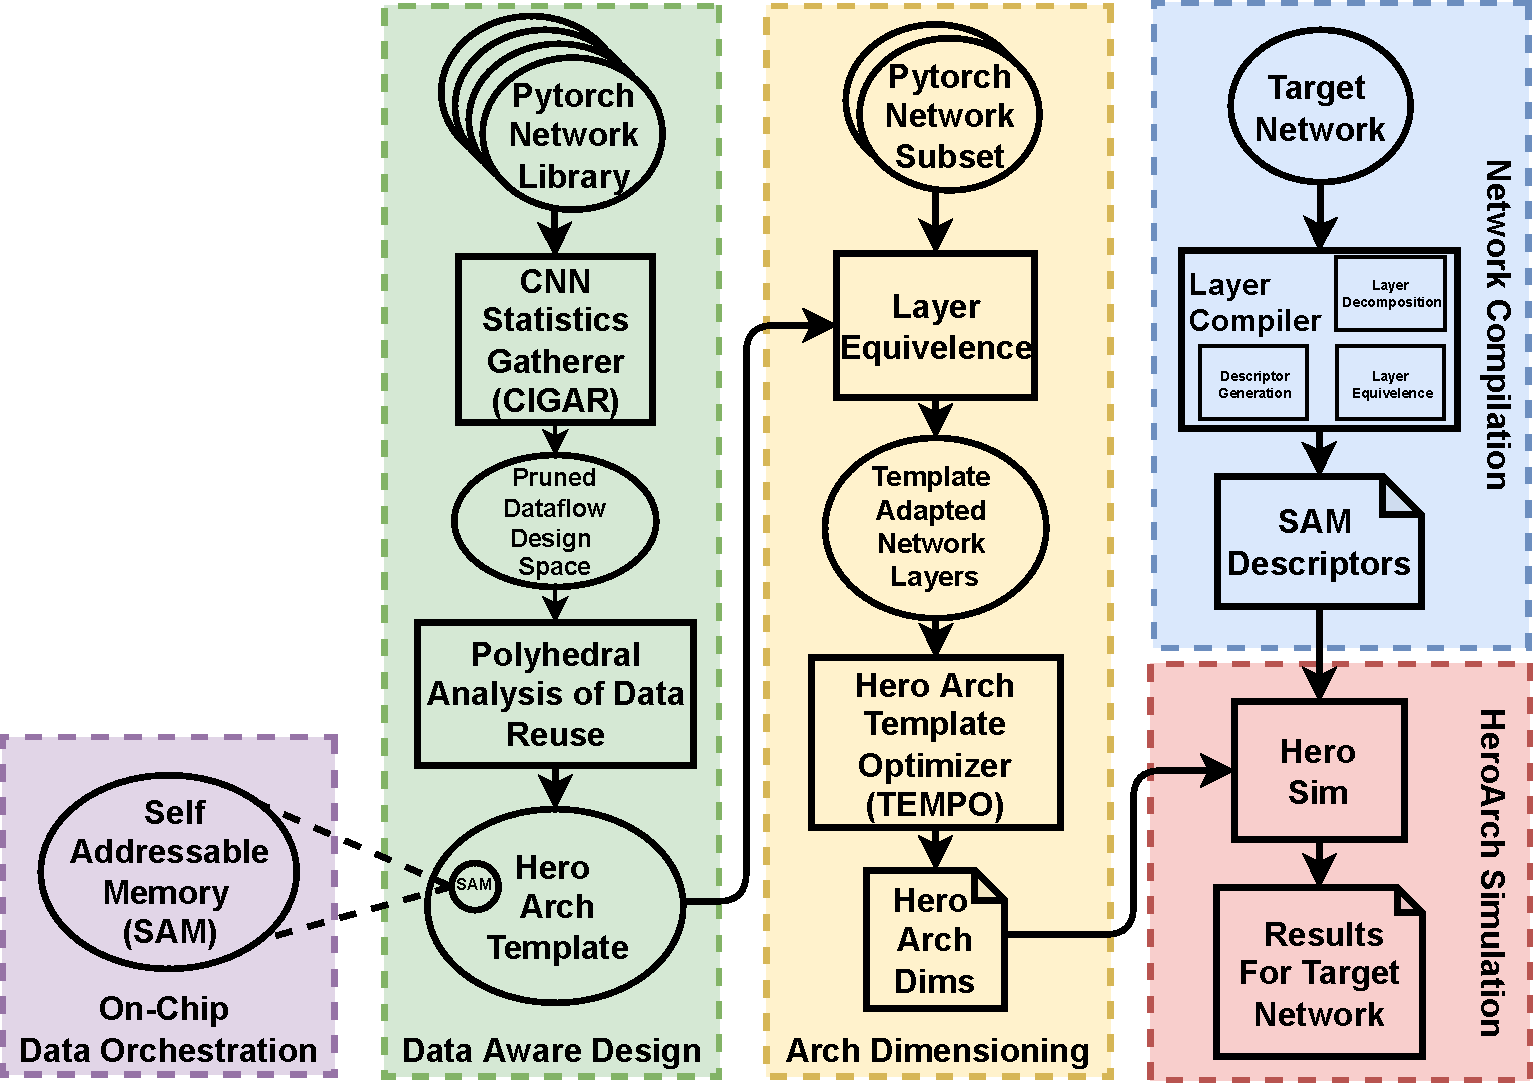
\includegraphics[scale=1]{fig/intro.pdf}
  \caption{Visual illustration of the solution overview}
  \label{fig:intro}
\end{figure}


The full solution overview is presented in \autoref{fig:intro}. This thesis
presents (HERO), a Hybrid GEMM and Direct Convolution Accelerator.  
HERO supports general matrix multiplication to maintain generality across
different network layers. General matrix multiplication is the backbone of many
computationally intensive layers in modern DNNs, for example, self attention
layers in transformer networks \cite{transformer_model} as well as fully
connected layers in many CNNs like Resnet \cite{resnet}. Extending support to
GEMM should not detract from the primary goal of accelerating convolutions since
they represent a larger portion of most network's runtime.  
HERO is derived from a data aware design process. It is optimized for the common
case of convolutions in the literature by supporting these convolution
configurations directly without the need to convert them into GEMM using data
transformation techniques like Im2Col.


To find the common case of convolutions,
this thesis introduces \ac{CIGAR}. CIGAR can gather configuration statistics for
convolution and linear layers in a libray of DNNs networks written in PyTorch
\cite{pytorch}. The heart of CIGAR is it's model dim collector that can collect
convolution and linear layer configuration for any network written in pytorch.
CIGAR can analyze a network or a library of networks and reveal the most common
convolution layer configurations (e.g their kernel and stride sizes) across the
entire library. The networks analyzed by CIGAR are all provided by the \ac{TIMM}
python library of networks \cite{timm}, which has over 695 networks written in
pytorch available for analysis. Convolution layer configurations that are not
supported directly by the architecture are converted into equivalent GEMM
operations using data transformation techniques like Im2Col
\cite{cafe_con_troll}. 
This thesis introduces the Hybrid GEMM and Direct Convolution Accelerator
(HERO), a neural network accelerator that balances generality and efficiency in
its design. HERO supports general matrix multiplication, the backbone of many
computationally intensive layers in modern DNNs, without detracting from its
primary goal of accelerating convolutions.

HERO's design is data-aware, optimized for the common case of convolutions by
supporting common configurations directly without the need for conversion
techniques like Im2Col. To identify the common case of convolutions, this thesis
introduces CIGAR, a tool that can gather configuration statistics for
convolution and linear layers in a library of DNNs written in \cite{pytorch}. CIGAR can
analyze a network or a library of networks and reveal the most common
convolution layer configurations across the entire library. The networks
analyzed by CIGAR are provided by the \cite{timm} python library of networks, which has
over 695 networks written in PyTorch available for analysis. Any layer configurations
not supported directly by HERO are converted into equivalent GEMM operations
using data transformation techniques like Im2Col
\cite{cafe_con_troll}.


HERO is more than just a single architecture; it represents a configurable
template with flexible allocation of on-chip compute resources for processing
convolution layer channels and filters. This configurability allows for
compile-time optimization of HERO by changing the number of PEs allocated to
processing different channels and filters in a convolution layer. To determine
the optimal configuration, this thesis introduces TEMPO, a tool that uses
analytical models for estimating different architecture metrics like latency,
utilization, and memory access counts when running different DNNs. TEMPO takes
advantage of CIGAR's model dimension collection to extract configurations of
convolution layers and applies the aforementioned analytical models to them.
TEMPO provides the initial architecture dimensions for the HERO template in
order to get the first estimates for other performance metrics. TEMPO only
defines layer dimensions for channel and filter concurrency. A separate analysis
of memory usage for different convolution elements is provided in this thesis.
The networks  used by TEMPO is the entire TIMM library to find the most general
architecture dimensions for HERO.


This thesis introduces the Self-Addressable Memory (SAM), an on-chip
programmable memory primitive, to manage data movement within the Hybrid GEMM
and Direct Convolution Accelerator (HERO). SAMs are programmed using descriptors
that define time-dependent address streams, which, in combination with
sufficiently flexible on-chip communication, provide the necessary flexibility
to map arbitrary network layers onto HERO. SAMs enable for more efficient data
movement on-chip, with the aim of maximizing data reuse. To determine the reuse
behavior in the convolution operation, this thesis applies the polyhedral model
to different data elements in convolution layers, using techniques outlined in
\cite{meeus}. Additionally, this thesis introduces a HERO network compiler
called EMPIRE that aids in the mapping of arbitrary PyTorch models to SAM
descriptors, which drive on-chip data movement.


To evaluate the performance and energy efficiency of HERO, a cycle accurate
simulation platform is developed. This simulation platform is driven by a
SystemC simulation backend and a Python evaluation frontend. The simulation
platform allows for the evaluation of different configurations of HERO on a wide
variety of networks. An analysis of an optimal HERO configuration when running
695 networks from the TIMM library was performed. The HERO configuration
analyzed was found to perform well on a wide variety of network configurations,
achieving a median FPS of ~91 FPS with a median speedup of 4.87X over CPU
baseline. The estimated bandwidth required for the configuration of HERO studied
was 19.65GiB/s which is within the PC4-21300 DDR4 specification. With that
configuration of DRAM, the median inferences/J is 57. The total on-chip area is
estimated at 0.34 $mm^2$.

Overall, HERO provides a high-performance, energy-efficient solution for
accelerating convolution layers in a wide range of DNNs. Its general
architecture and support for GEMM, in addition to its direct support for the
common case of convolution layers, make it a versatile accelerator that can
adapt to changing trends in DNNs. The introduction of CIGAR and the HERO layer
compiler, in addition to the use of SAM, further improves the design process and
ease of use of HERO. The cycle accurate simulation platform developed allows for
the accurate evaluation of HERO's performance


\section{Thesis Structure}
\label{chap:intro:thesis_structure}


In this thesis, Chapter \ref{chap:background:intro} discusses background and
related work in the literature. Chapter \ref{chap:dda} introduces the CIGAR and
the data-aware design approach from which HERO is derived. Chapter
\ref{chap:arch_dimensioning} introduces TEMPO, from which several candidate
configurations of HERO are presented. Chapter \ref{chap:data_orchestration}
introduces the SAM primitive. Chapter \ref{chap:net_compile} discusses HERO's
network compilation process and how SAM descriptors are generated from arbitrary
models in Pytorch using EMPIRE. Finally, Chapter \ref{chap:hero:sim_platform}
discusses the HERO simulation platform as well as results from running a HERO
configuration optimized by TEMPO on all 695 networks in the TIMM library.

\chapter{Background}
\label{chap:background:intro}

To motivate the architecture design space introduce in chapter (REFERENCE chapter)
I first need to 
3) show how to convert a convolution operation into a GEMM
4) Introduce dataflow exploration through direct representation if implementing
an accelerates that accelerates convolutions directly
5) Introduce hardware 
+ based on reuse behavior in the Dataflow
dataflow -> describes communication -> describes datareuse
6) Introduce polyhedral model to evaluate temporal reuse behavior
In this chapter I
breakdown what convolutions are mathetmatically


\figref{fig:cnn_network}

\begin{figure}[ht]
    \centering
    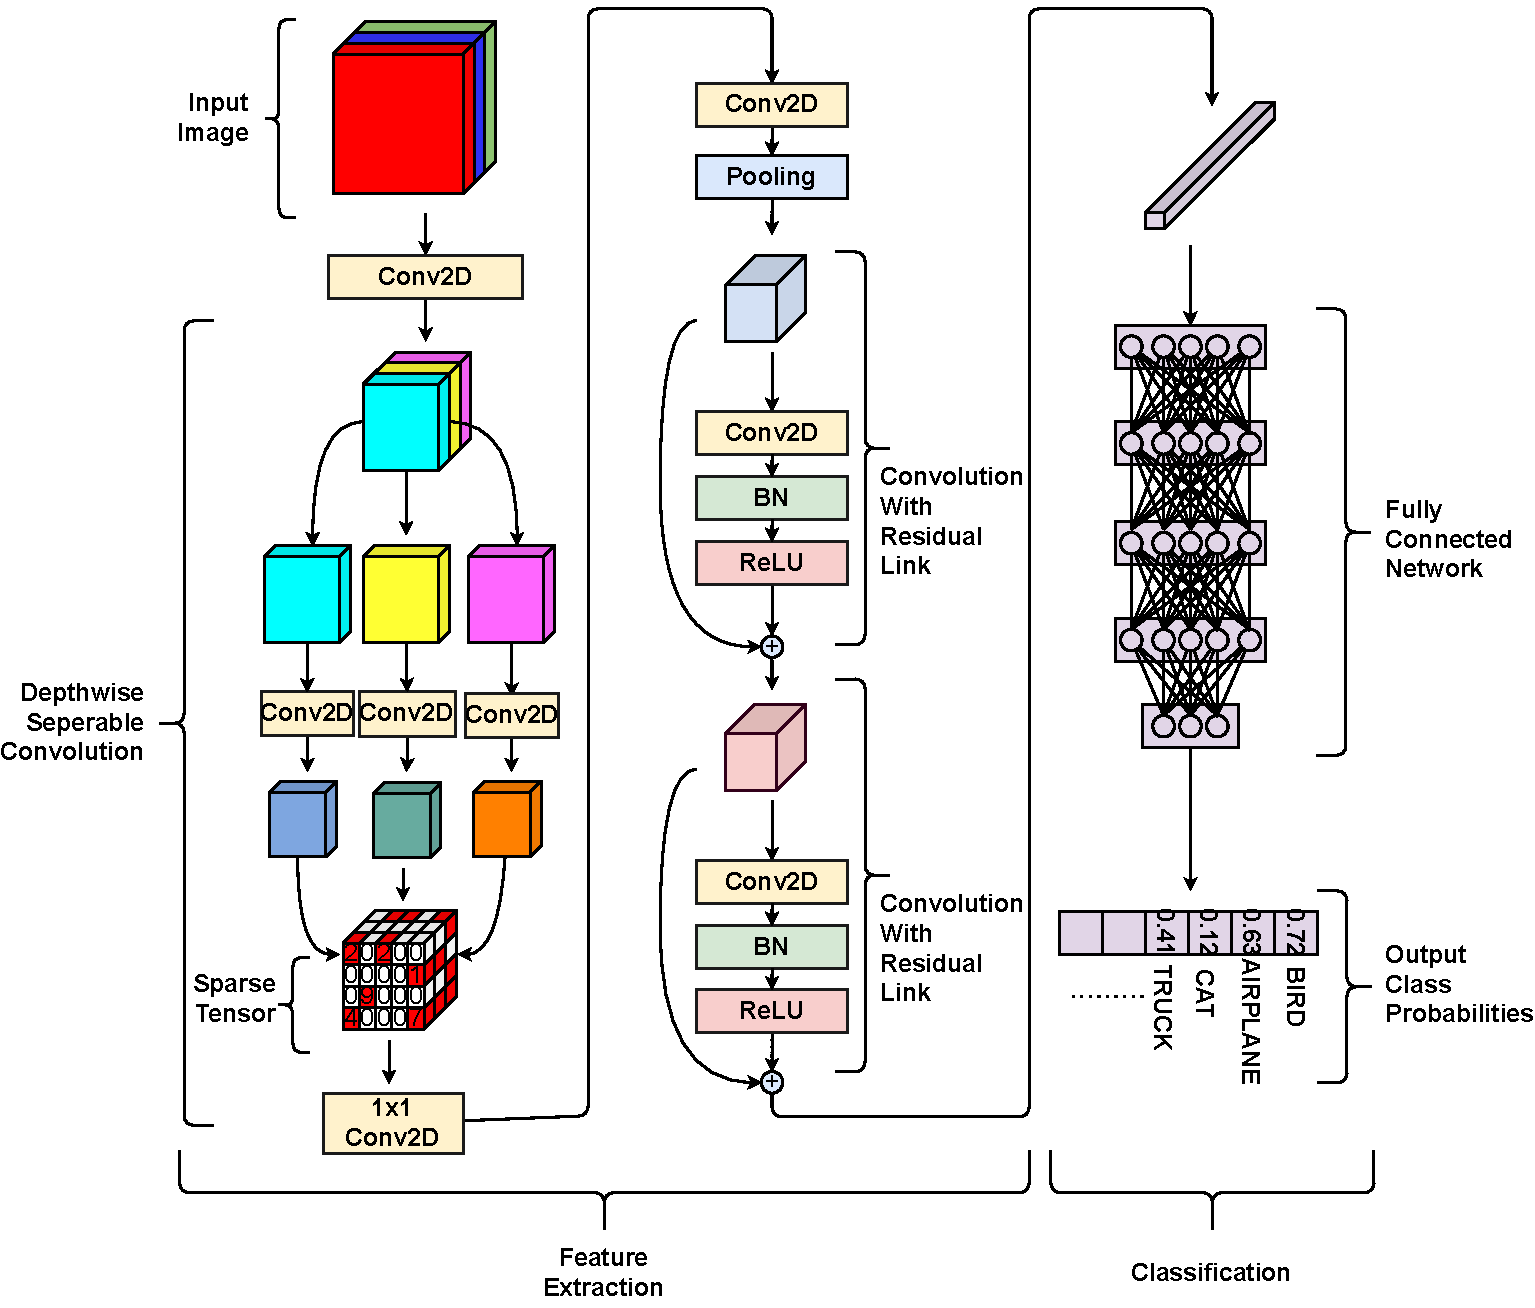
\includegraphics[scale=0.4]{fig/cnn.pdf}
    \caption{Example Image Classfication CNN}
    \label{fig:cnn_network}
\end{figure}

\clearpage

\section{The Math behind convolutions}
\label{chap:intro:conv_operation}

1) explain what convolutions are mathematically

\begin{figure}[ht]
    \centering
    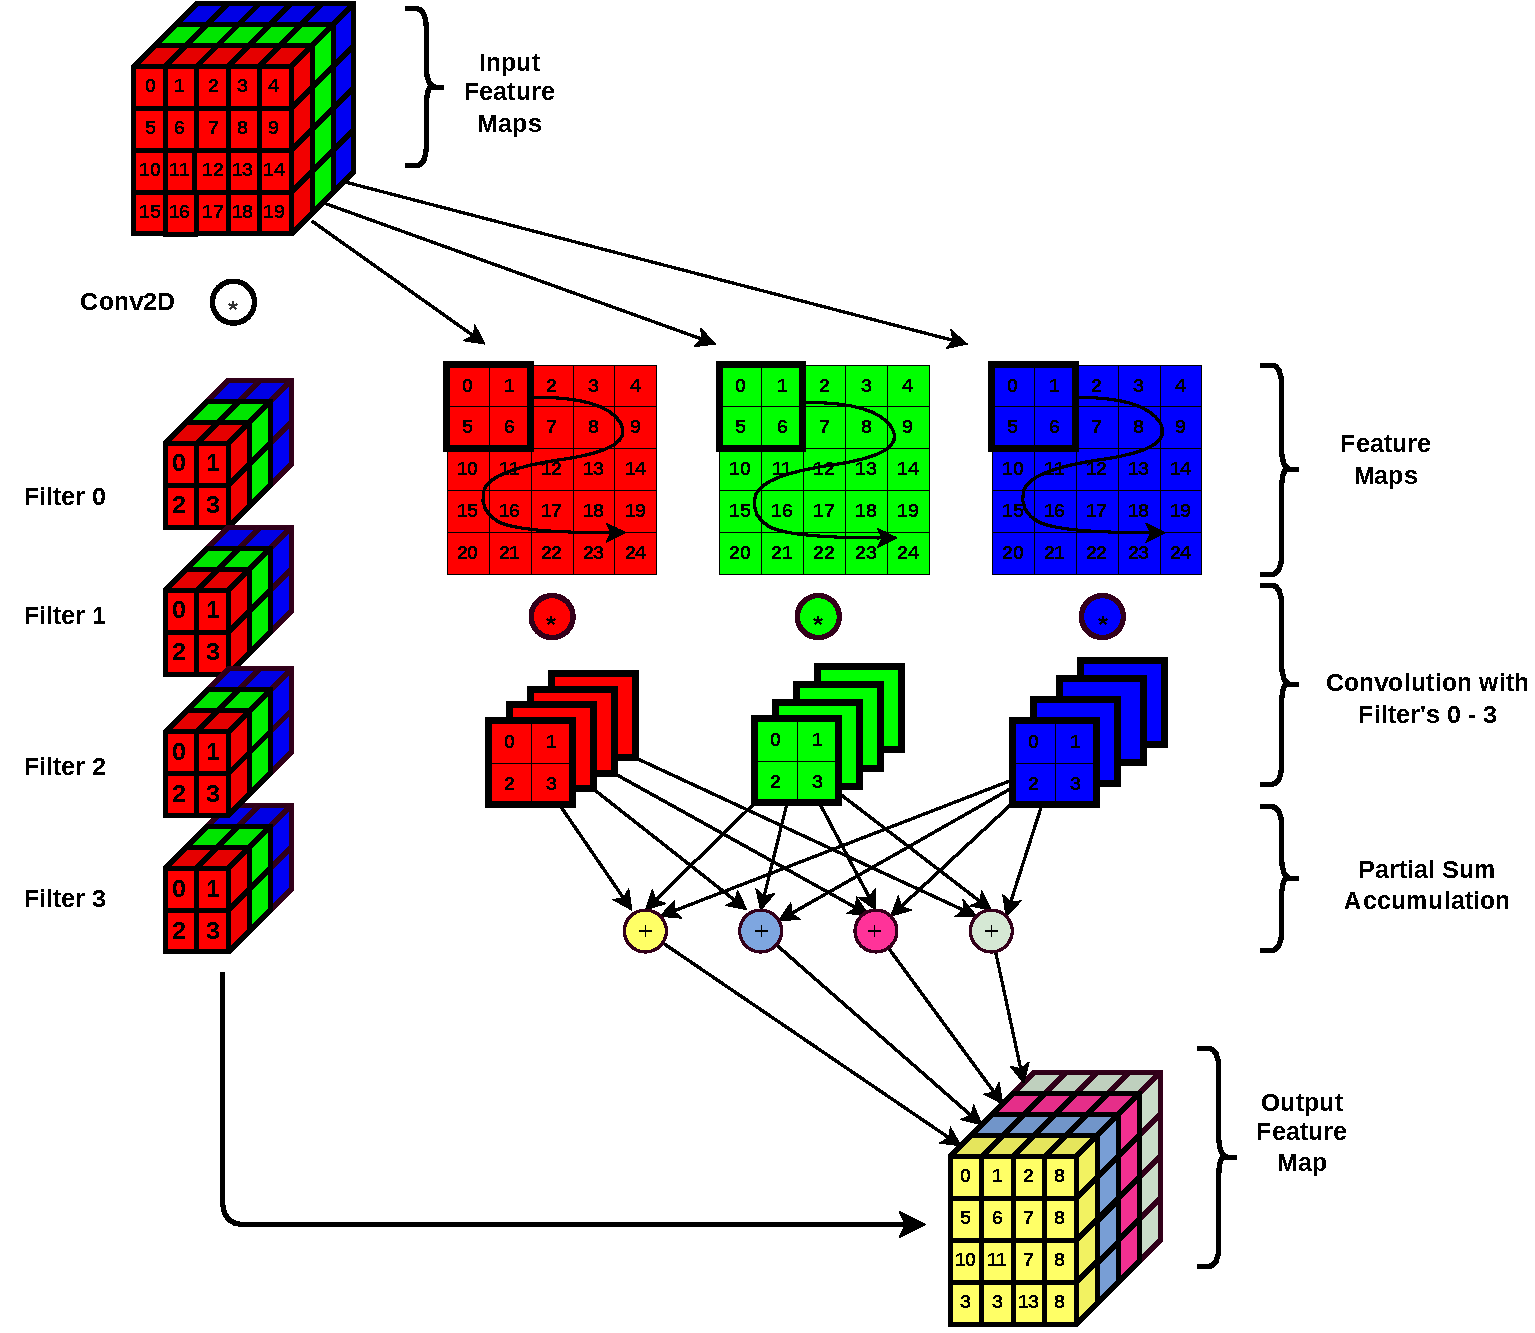
\includegraphics[scale=0.6]{fig/ConvExplained.pdf}
    \caption{Convolution Operation Illustrated}
    \label{fig:conv_explained}
\end{figure}

\begin{align}
    \begin{split}
        IFmap \in R^{C \times n\times n} \\
        OFmap \in  R^{F \times m\times m} \\
        Weight \in R^{F \times C\times K\times K} \\
    \end{split}
    \label{math:default_tensor_def}
\end{align}

\begin{align}
    OFmap[f][y][x] = \displaystyle\sum\limits_{c=0}^{C-1}\displaystyle\sum\limits_{k_x=0}^{K-1}\displaystyle\sum\limits_{k_y=0}^{K-1}Weight[f][c][k_y][k_x]*IFmap[c][y+ky][x+kx]
    \label{math:conv_equation_1fp}
\end{align}

\section{Loop Based Representation Of Convolutions}
\label{chap:intro:conv_operation}

Direct naive implementation of \autoref{math:conv_equation} with tensors
\autoref{math:default_tensor_def} as a series of loops is given below
\autoref{lst:conv_loop}

\begin{minipage}{\linewidth}
    \begin{lstlisting}[language=C, caption=Convolution implemented as nested loops, label={lst:conv_loop}]
for(int f = 0; f < F; f++) // Filter loop
    for(int c = 0; c < C; c++) // Channel loop
        for(int y = 0; y < Y; y++) // Output feature map row
            for(int x = 0; x < X; x++)  // Output feature map col
                for(int ky = 0; ky < KY; ky++)  // Kernel row
                    for(int kx = 0; kx < KX; kx++)  // Kernel col
                        O[f][y][x] += I[c][y+ky][x+kx]*W[f][c][ky][kx];
    \end{lstlisting}
\end{minipage}

\newpage

\section{Convolution as general matrix multiplication}
\label{chap:intro:conv_operation}

\begin{figure}[ht]
    \centering
    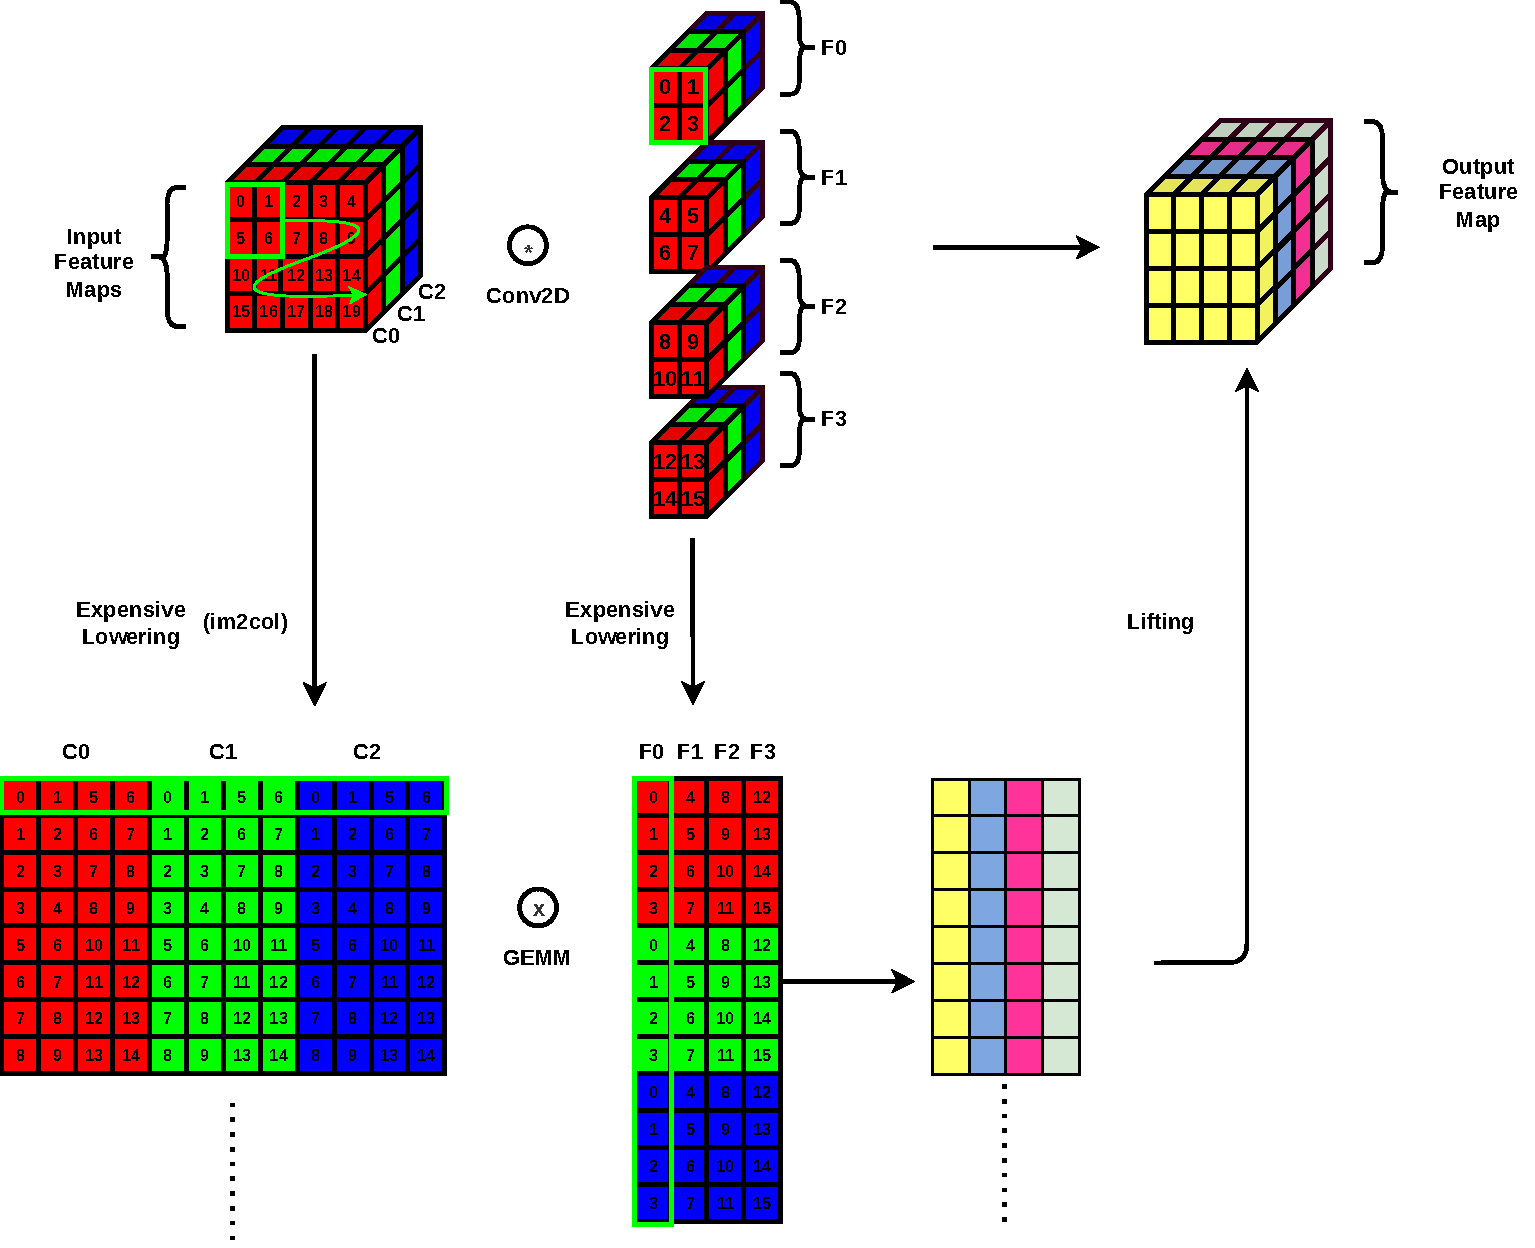
\includegraphics[scale=0.6]{fig/Im2Col.pdf}
    \caption{Im2Col Illustrated}
    \label{fig:im2col}
\end{figure}

Convolution can be converted into a \ac{GEMM}

Popular techniques like im2col (illustrated in \autoref{fig:im2col}) can be used
to convert any convolution operation into \ac{GEMM} (listed as expensive
lowering \cite{cafe_con_troll}) but there are others techniques that don't
produce such massive input feature maps


If willing to increase complexity of lowering of ifmap and weight tensors after
GEMM we can reduce bloat in ifmap with balanced lifting/ loading in
\cite{cafe_con_troll}. Analytical expressions adapted from \cite{cafe_con_troll}
are given below with the inclusion of lowering in the presence of multiple
filters.


\clearpage

\begin{align}
    \begin{gathered}
        IFmap \in R^{C\times n\times n} \xrightarrow[]{Balanced Lowering} \hat{IFmap} \in R^{nm\times KC} \\
        \hat{IFmap}[cn+r, :] = vec(IFmap[:, r, c:c+K]) \\
        \forall r,c \in [0, n-1], [0, m-1]
    \end{gathered}
    \label{math:balanced_lowering_ifmap}
\end{align}

\begin{align}
    \begin{gathered}
        Weight \in R^{F\times C\times K \times K} \xrightarrow[]{Balanced Lowering} \hat{Weight} \in R^{KC\times FK}\\
        \hat{Weight}[f*K:f*K+K, i] = vec(Weight[f, :, i, :]) \\
        \forall f,i \in [0, F-1], [0, K-1]
    \end{gathered}
    \label{math:balanced_lowering_weight}
\end{align}
In balanced lowering, we first lower the ifmap and weights using expression 
\eqref{math:balanced_lowering_ifmap} and \eqref{math:balanced_lowering_weight}.

\begin{align}
    \begin{gathered}
        \hat{OFmap} = \hat{IFmap}.\hat{Weight}
    \end{gathered}
    \label{math:balanced_lowering_gemm}
\end{align}
Then a \ac{GEMM} is performed \eqref{math:balanced_lowering_gemm}


\begin{align}
    \begin{gathered}
        \hat{OFmap} \in R^{nm\times FK} \xrightarrow[]{Balanced Lifting} OFmap \in  R^{m\times m\times F}\\
        OFmap[f, r, c] = (\displaystyle\sum\limits_{j=0}^{K-1} \hat{OFmap}[cn+r+j, j+fK]) \\
        \forall f,r,c \in [0, F-1], [0, m-1], [0, m-1]
    \end{gathered}
    \label{math:balanced_lifting_ofmap}
\end{align}

Followed by a lift operation on the output $\hat{OFmap}$ matrix using \eqref{math:balanced_lifting_ofmap}

Illustration of this data transformation is presented in \autoref{fig:balanced_lowering_lifting}

Pros of lowering/ lifting

Conv as GEMM Offers the most flexibility because it’s insensitive to changes in
convolution parameters

It also allows leaves us with a GEMM accelerator which is useful for many other
NN layers e.g Linear/ Self attention/ LSTM

Con is that it still causes bloat in ifmap and additionaly complexity/ latency of 
lifting/ lowering. Which in the balanced case is $m^{2}K$ \cite{cafe_con_troll}

\begin{figure}[!ht]
    \centering
    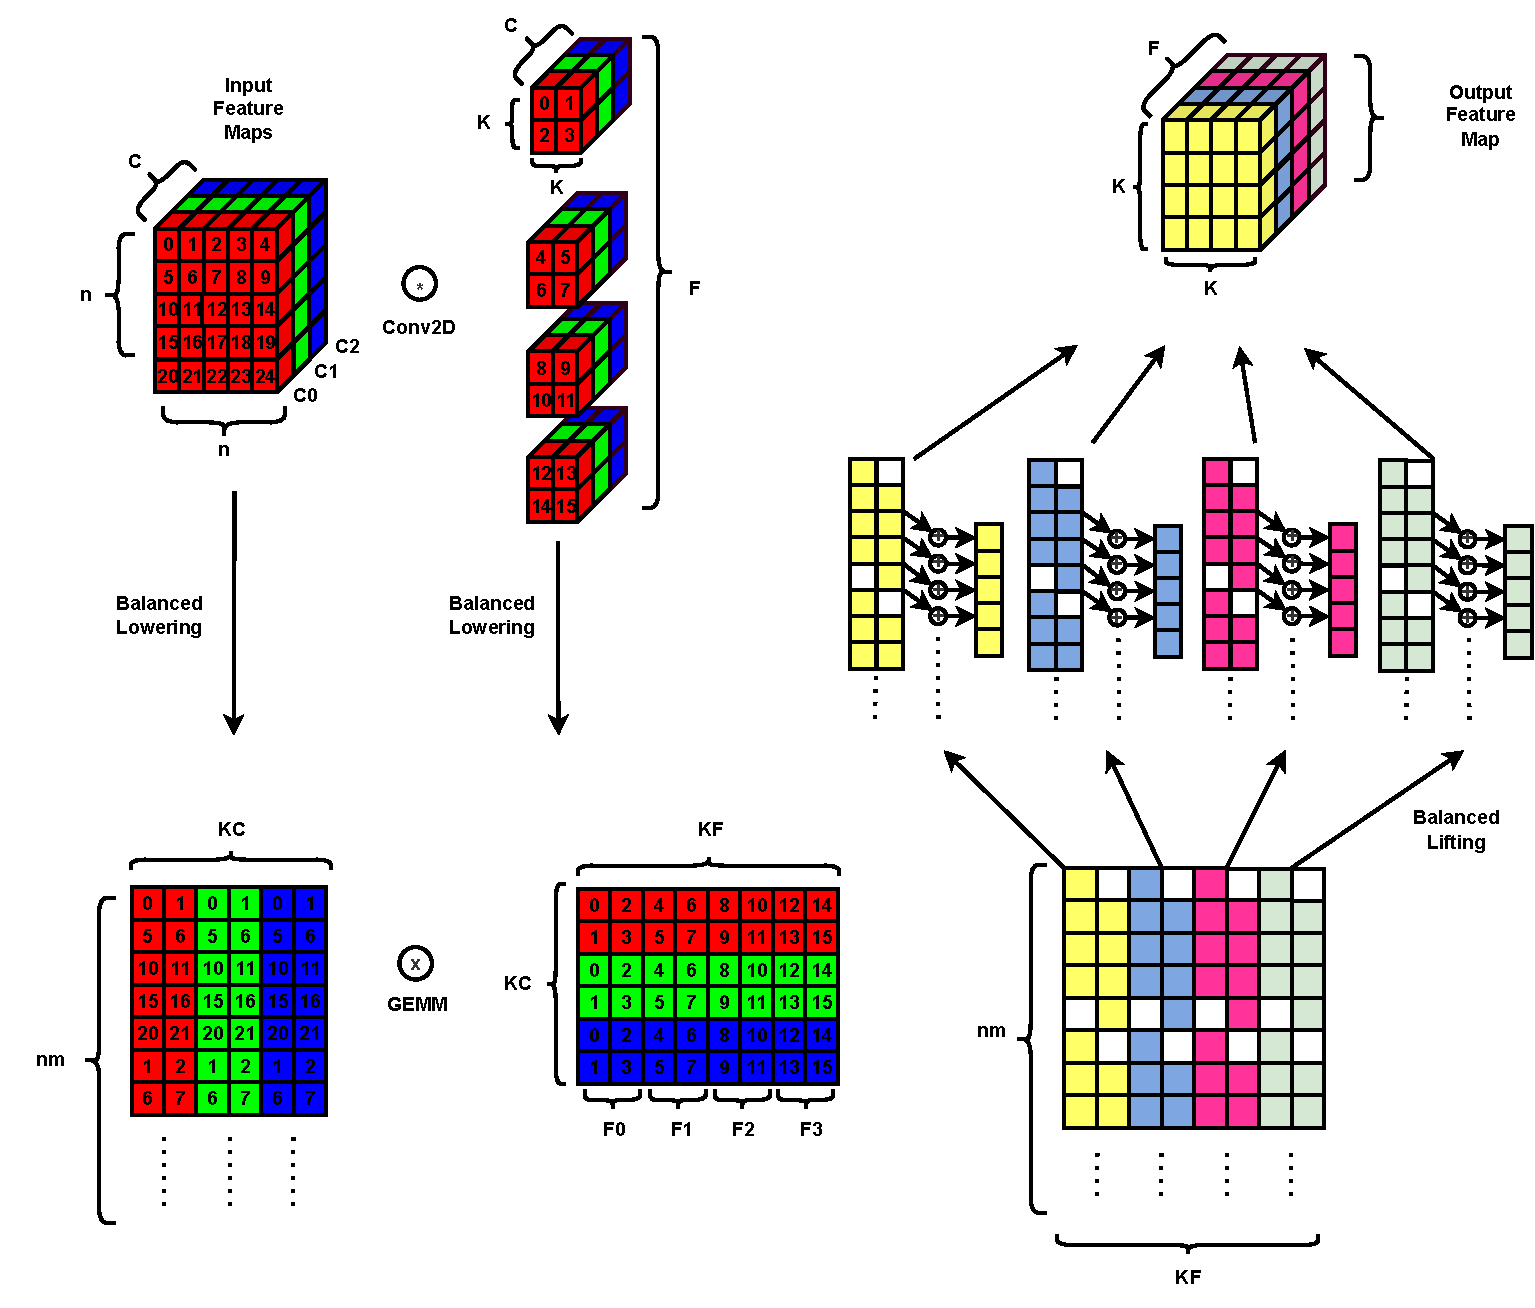
\includegraphics[scale=0.6]{fig/BalancedLoweringLifting.pdf}
    \caption{Balanced Lowering/Lifting Illustrated}
    \label{fig:balanced_lowering_lifting}
\end{figure}


\section{Implementing convolutions in hardware}
\subsection{The dataflow taxonomy}

In the dataflow design space, from \cite{dnn_df_overrated} 
dataflows can be represented using the direct convolution
nested loop structure combined with unroll pragmas. Listing \ref{lst:W_S_Generic_Loop} shows a generic
implementation of a single convolution layer as a loop structure under a weight
stationary dataflow configuration. What defines that dataflow is 1) loop unroll
targets 2) loop order 3) the unroll factors of the unrolled loops. Weight elements within a
kernel remain stationary throughout the computation of an output feature map
until a new tile of channels C\_T is loaded into the accelerator. Once the
weights within a particular channel and filter group are used to produce an
output feature map they are discarded and are only loaded again when computing
the same layer for a new input image. From listing \ref{lst:W_S_Generic_Loop} we
can see that from the loop unroll targets and loop unroll factors there are many
other possible dataflow configurations available to us outside of weight
stationary. Additionally, since accelerators are generally limited to two
spatial axis the loops of the convolution operation can be mapped to two spatial
axis. If we allow multiple convolution loops under some kernel unroll factor
KY\_T/KX\_T  to be unrolled and mapped to the same accelerator spatial axis we
can influence the effective unroll factors when performing different
convolutions of different kernel sizes other than KY\_T/KX\_T. The choice of
which loops are mapped to which spatial axis is an additional design dimension
alongside loop unrolling. To summarize, from the loop representation of
convolution accelerator dataflows we have three design space dimensions, 1) Loop
unroll targets 2) Loop unroll factors 3) Loop spatial mapping. Given the size of
this dataflow design space we will use CIGAR and Tempo to derive the common
case for convolution layers and limit the scope of the dataflow design space.

CNN layer loops + loop ordering + Loop tilings can express different
accelerators dataflows like row stationary, weight stationary, etc



\begin{minipage}{\linewidth}
    \begin{lstlisting}[language=C, caption=Convolution implemented as nested loops, label={lst:conv_loop}]
#pragma UNROLL F_T
for(int f = 0; f < F; f+=F_T) // Filter loop
#pragma UNROLL C_T
    for(int c = 0; c < C; c+=C_T) // Channel loop
#pragma UNROLL Y_T
        for(int y = 0; y < Y; y+=Y_T) // Output feature map row
#pragma UNROLL X_T
            for(int x = 0; x < X; x+=X_T)  // Output feature map col
#pragma UNROLL KY_T
                for(int ky = 0; ky < KY; ky+=KY_T)  // Kernel row
#pragma UNROLL KX_T
                    for(int kx = 0; kx < KX; kx+=KX_T)  // Kernel col
                        O[f][y][x] += I[c][y+ky][x+kx]*W[f][c][ky][kx];
    \end{lstlisting}
\end{minipage}


\begin{figure}
    \centering
    \subfigure[]{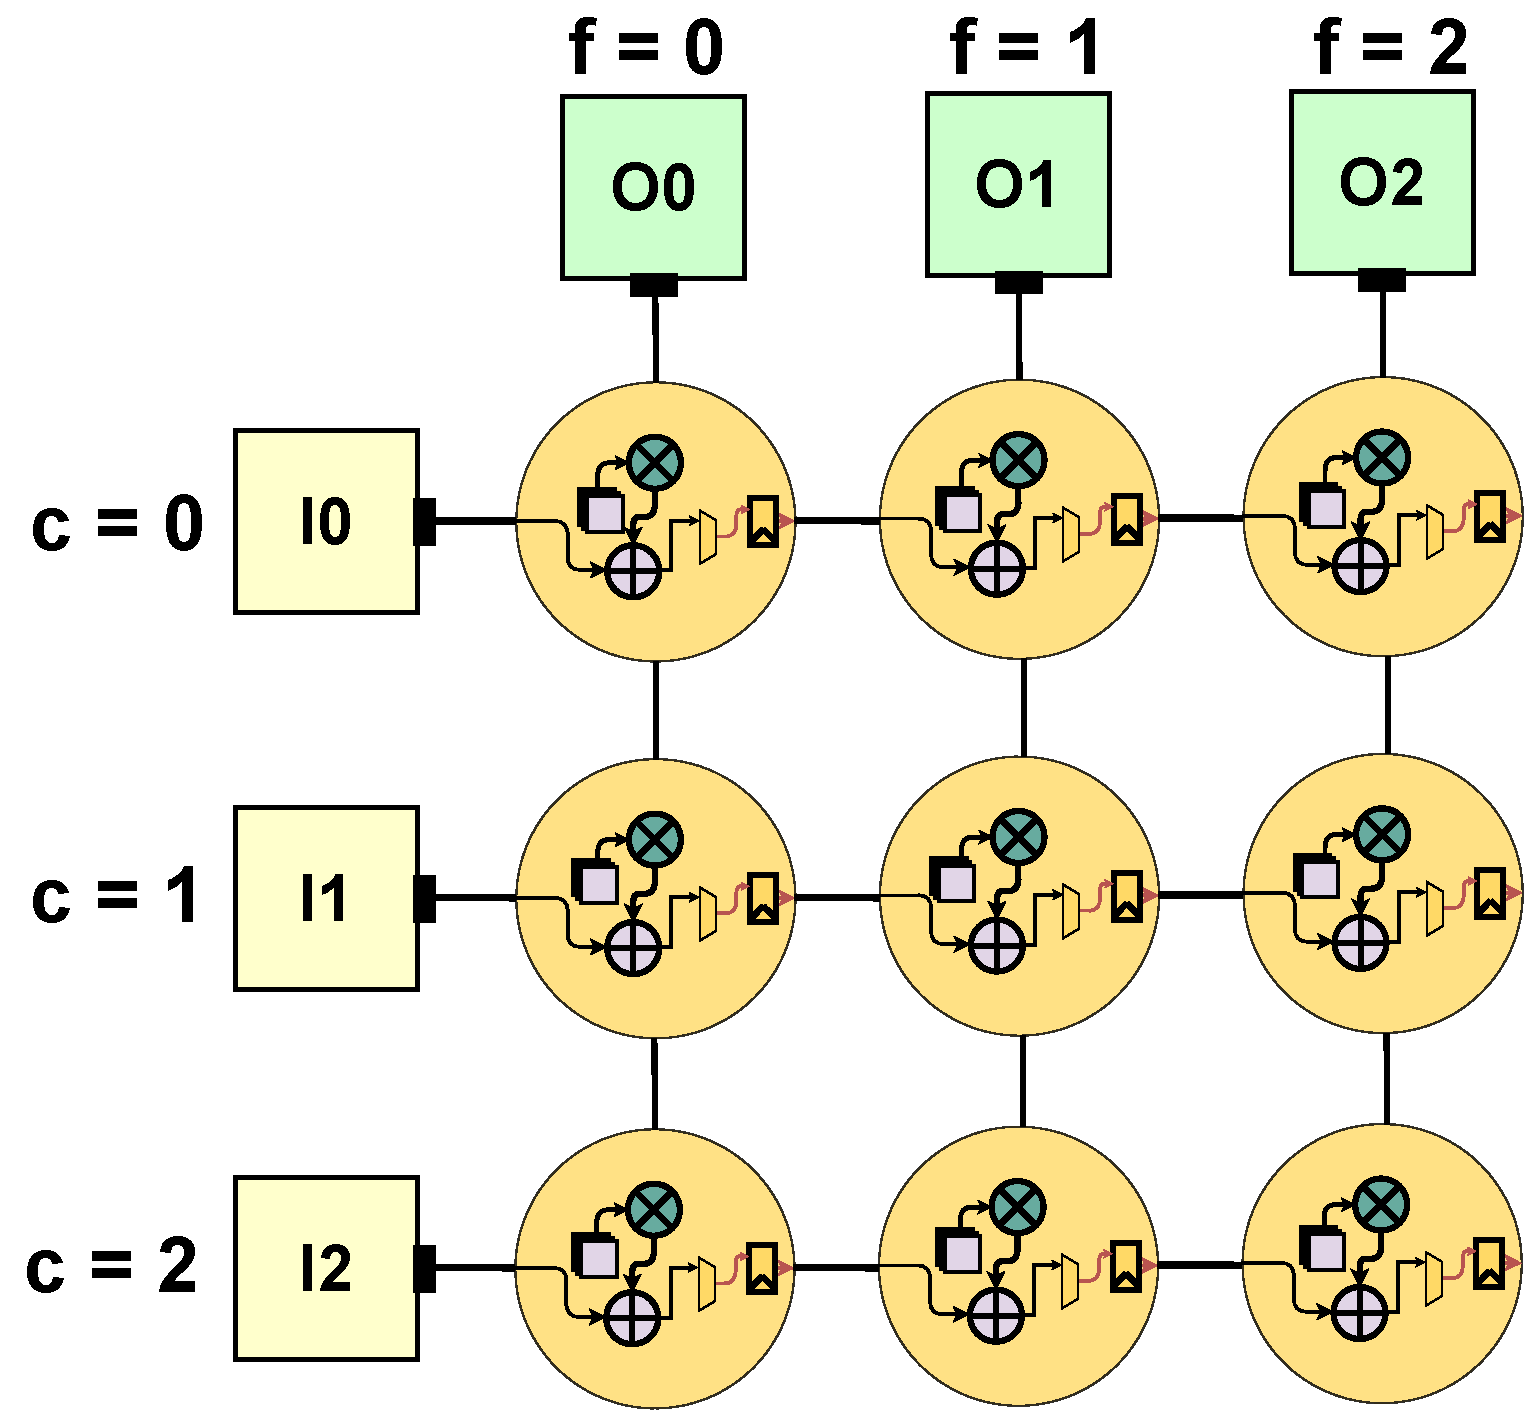
\includegraphics[width=0.32\textwidth]{fig/unroll_c_f.pdf}}
    \hspace{0.1cm} 
    \subfigure[]{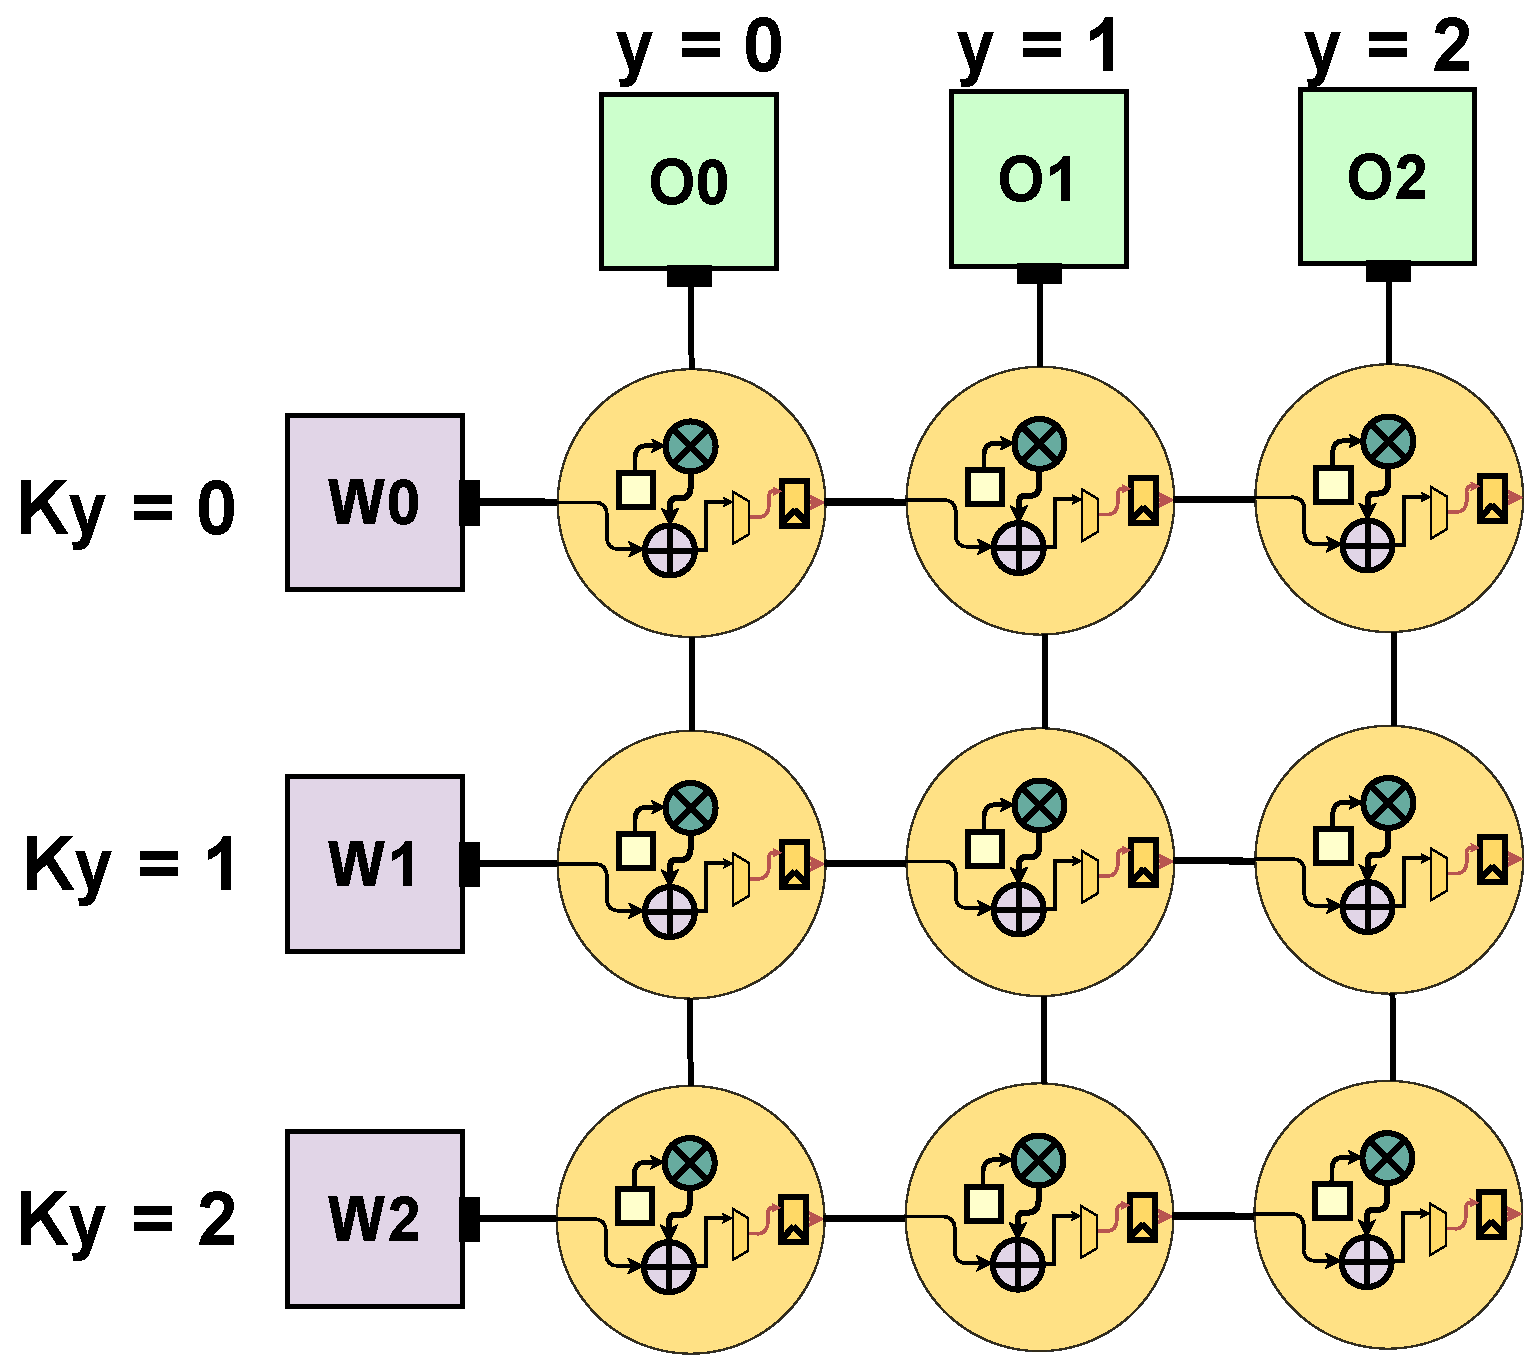
\includegraphics[width=0.32\textwidth]{fig/unroll_fy_y.pdf}}
    \hspace{0.1cm} 
    \subfigure[]{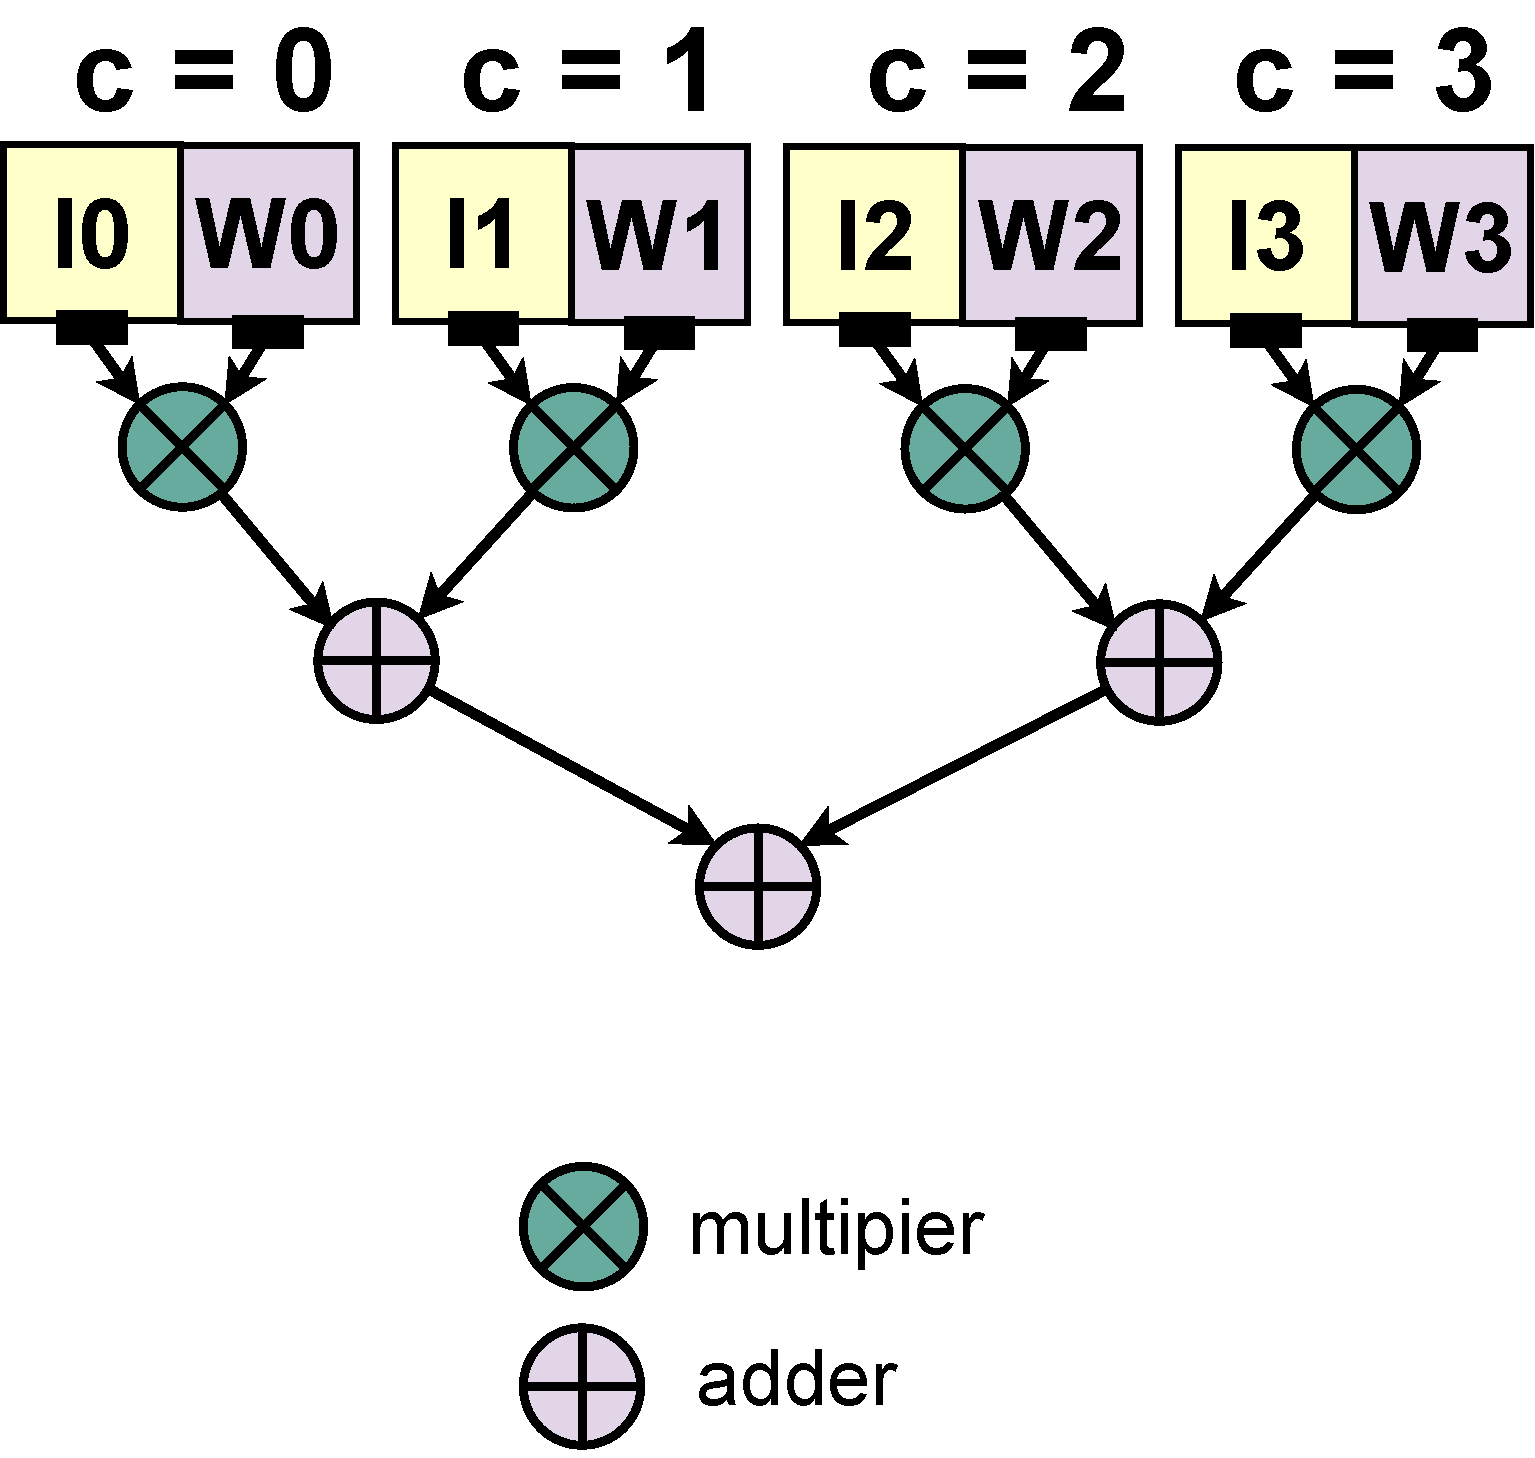
\includegraphics[width=0.32\textwidth]{fig/unroll_c.pdf}} 
    \hspace{0.1cm} 
    \subfigure[]{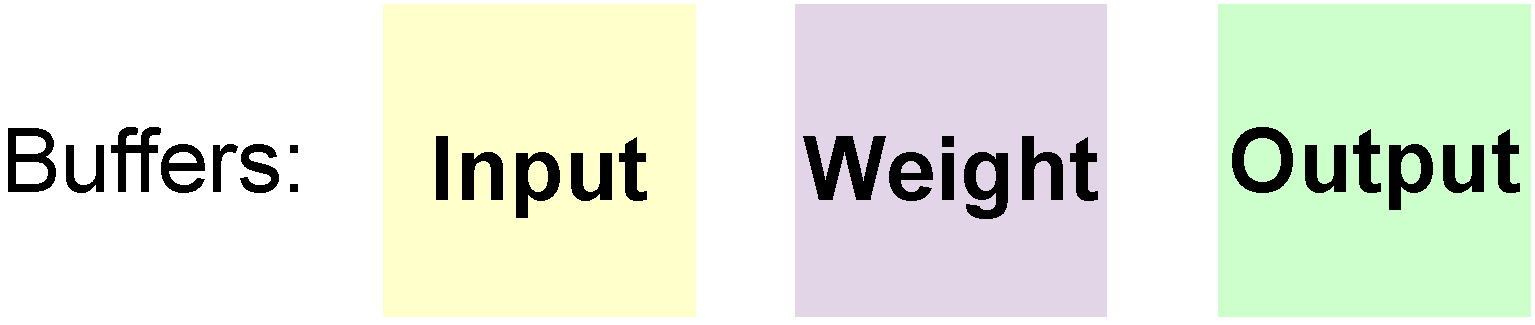
\includegraphics[width=0.3\textwidth]{fig/buffer_description.pdf}}
    \caption{Illustration of different dataflow implementations adapted from \cite{dnn_df_overrated} (a) blah (b) blah (c) blah (d) blah}
    \label{fig:unroll_illustration}
\end{figure}


From dataflow we can derive hw implementation based on communication pattern and
reuse behavior of the individual data elements accessed in the convolution
layer.

\subsection{The Hardware Implementation taxonomy}

Figures in \autoref{fig:unroll_illustration} show different reduction/ multicast
schemes based on reuse behavior of data elements (IFmap, OFmap, Weights)
apparent in the dataflow. The space of available schemes is not limited to those
presented in \autoref{fig:unroll_illustration} though. In \cite{maestro} a
hardware taxonomy illustrated in figure \autoref{fig:hw_taxonpmy}.

\begin{figure}[ht]
    \centering
    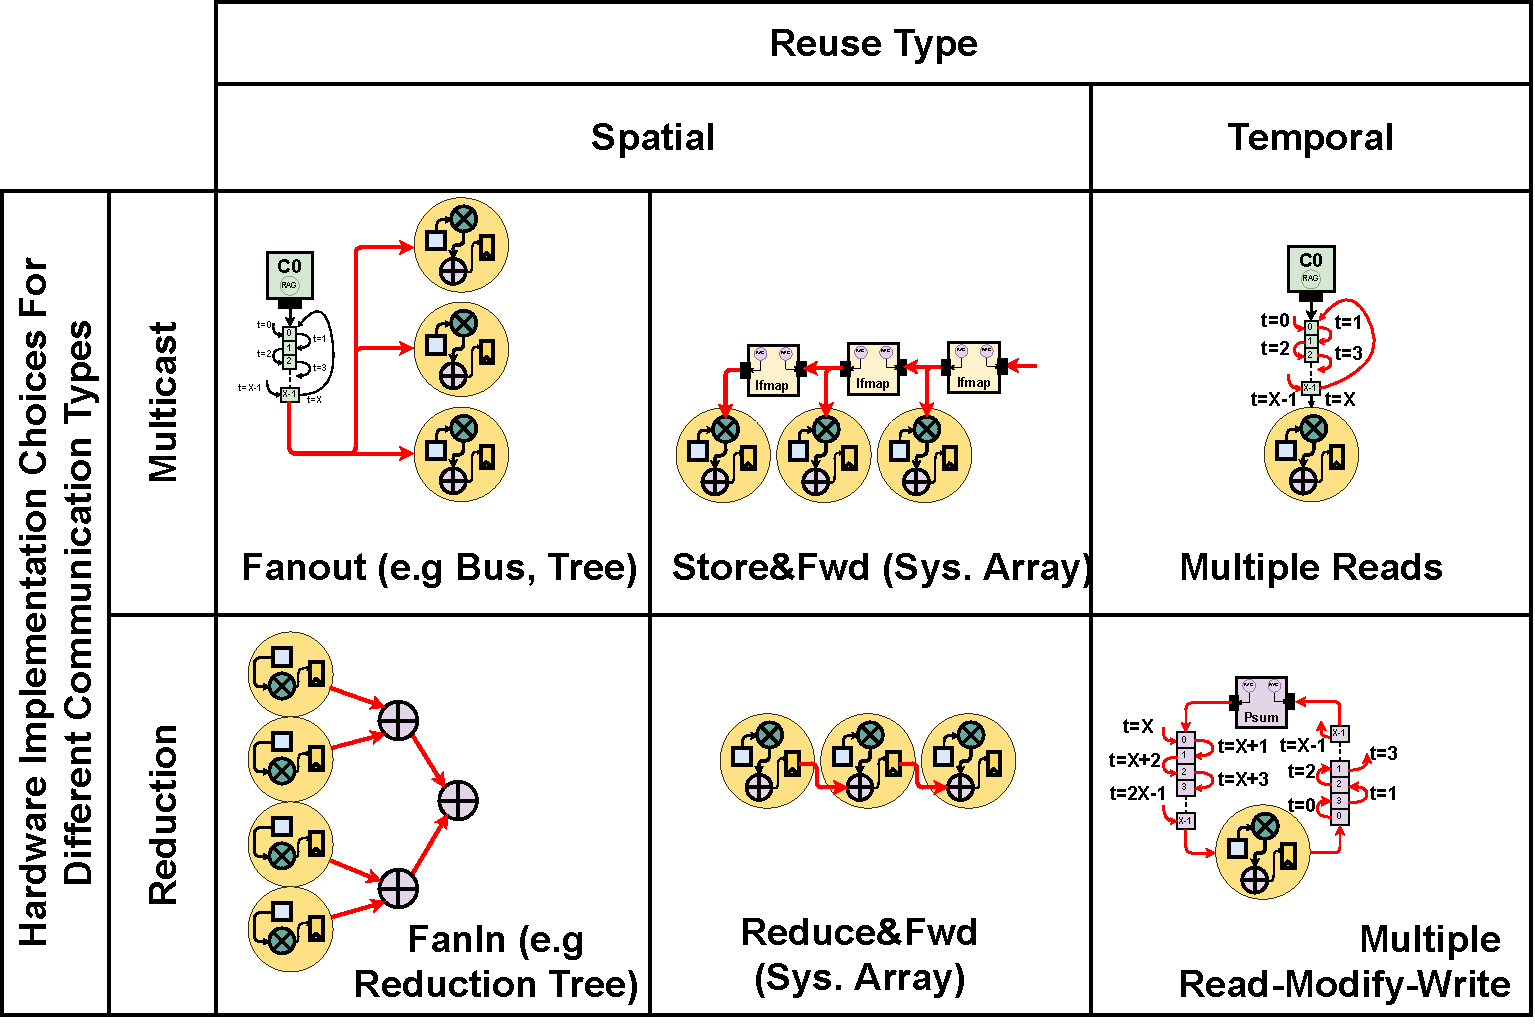
\includegraphics[scale=0.58]{fig/hw_taxonomy.pdf}
    \caption{Hardware Implementation Taxonomy adapted from \cite{maestro}}
    \label{fig:hw_taxonomy}
\end{figure}


Depending on the dataflow described using the dataflow taxonomy (1) loop
ordering (2) unroll targets (2) loop unroll factors. The implementation options
are derived based on the type of reuse present in the dataflow. Following the
hardware implementation taxonomy presented in in \cite{maestro}, we can classify
the available hardware implementation options based on the the type of reuse is
spatial (reuse distance = 0) or temporal (reuse distance > 0) that exists for a
given data element accessed in the dataflow. Within a reuse type, depending on
the nature of the reuse, if it is read or read modify write, there are several
options for supporting the communication inferred from the reuse. To deduce the
type of reuse and overall communicaiton behavior for each data element in any
dataflow we can use the polyhedral model to detect temporal reuse. Spatial reuse
detection can be inferred directly from the loops.


\section{Analysis of data reuse with the polyhedral model}

\cite{meeus} used polyehdral model to analyse reuse within stencil based applications described
as nested loops. One important element in their approach is their program written in iscc that
can determine temporal reuse of data elements

There's the polyhedral extraction tool out there but unfortunately there's no
way to encode parallelism or loop unrolling in it without relying on compiler
pragmas. 

below is an example of this reuse applied to the gemm loops





% \chapter{Finding the common case for convolutions in CNNs with a CIGAR}



\chapter{Data-Aware Accelerator Dataflow Design Space Exploration}
\label{chap:dataflow_dse:intro}

As discussed in \autoref{chap:background:intro}, any convolution accelerator can
be reduced into it's dataflow and hardware implementation choices. Based on the
dataflow exploration approach in \cite{dnn_df_overrated_v1} dataflows are
explorable through the nested loop structure that makes up a convolution
layer introduced in \autoref{chap:background:intro}.
The design space dimensions of dataflows is comprised of:
\begin{itemize}
    \item Loop ordering of the nested loops structure
    \item Loop unroll targets (which loops are unrolled and which are not) 
    \item Loop unroll factors for the loop unroll targets
    \item Mapping of loops to an accelerators spatial axis of which there are 2
\end{itemize}

Ideally dataflow design space exploration should be hardware implementation
agnostic. We can enumerate the size of the design space by examining the scope
of the afformentioned design space dimensions. Beginning with the choice of loop
unroll targets. One can choose to unroll only one loop or all loops with
varying unroll factors. Unrolling loops exposes opportunities for parallelism
when executing unrolled loops on an accelerator. Therefore the number of
possible combinations of loop unroll targets is
$\sum\limits_{l=1}^{6}\binom{6}{l}$ with a total of $6!$ possible orderings for
said loops. The space of possible loop unroll axis mappings is $\binom{l}{\min(2,
l)}$ depending on the chosen number of loops $l$ unrolled. The space of possible
unroll factors is then dictated by the upperbounds of the indexes in the loop
representation $max(F).max(C).max(Y).max(X).max(KY).max(KX)$ and the upperbound
of the available processing engines $Count_{pe}$. Some combination of upper
bounds are very unlikely to occur in real networks which limits the size of the
design space for loop unroll factors. However, when considering the
mapping of unrolled loops to an accelerator's spatial axis, the choice of unroll
factors becomes more complicated. When two loops are unrolled in the same
spatial axis, the effective unroll factor for each one of them may change when
processing a layer with a different convolution layer configuration than the one
assumed when unrolling the loops. For example, consider the following situation.
For a convolution layer with kernel size 3x3 and channel count 32, if the kernel
loops are unrolled fully with an unroll factor of 9, and the channel loops are
unrolled partially with an unroll factor of 4, and they were both mapped to the
same spatial axis, then the total number of processing engines allocated to that
spatial axis would be 36. After allocating those PEs, if we attempt to execute a
different convolution layer with a different configuration, for example, a 1x1
convolution layer with 32 channels, the allocated PEs would be underutilized because
the effective channel unroll factor would be 36 instead of 4 in the original
configuration.

In this chapter we will first prune the dataflow design space dimensions in
\autoref{chap:dataflow_dse:pruning} by determining the apprioriate loop ordering
and loop unroll targets and loop unroll factors using insights acquired from
\ac{CIGAR} a convolutional network analysis tool discussed in
\autoref{chap:dataflow_dse:pruning:cigar}. Then, given the complexity of
exploring loop unroll factors and loop axis mapping, an automated accelerator
Template optimizer TEMPO introduced in \autoref{chap:dataflow_dse:exploring} is
used to explore the the afformentioned design space dimensions to produce
utilization optimized accelerator template configurations. 

\section{Pruning the design space with CIGAR}
\label{chap:dataflow_dse:pruning}

\subsection{CIGAR: The ConvolutIon statIstics GAtherer}
\label{chap:dataflow_dse:pruning:cigar}

\subsubsection{Algorithm}
\label{chap:dataflow_dse:pruning:cigar:algo}

Psudocode for \ac{CIGAR}'s algorithm is presented in algorithm
\ref{alg:cigar_algo}. In algorithm \ref{alg:cigar_algo}, \ac{CIGAR} begins by
calling Collect\_Library\_Statistics after acquiring a dictionary of pytorch
models $modell_{dict}$. Collect\_Library\_Statistics then instantiates an empty
$model^{stats}_{dict}$ to be populated with model layer statistics . It then
instantiates a collector object that acts as a container for collected model
statistics. For each model, a new input image tensor is created based on the
requirements of the model being analyzed. If no special transformations are
required a default image tensor configuration is used where the width and the
height dimension of the image is set 224x224 with 3 RGB channels. After an image
tensor is created, Attach\_Collection\_Hooks is called to attach the collector
object's extract\_stats callback function or hook on each Conv2D layer present
in the model's layers. Attach\_Collection\_Hooks returns an array to each
attached hook to be later detached once the model under inspection is processed.
An illustration of this process is given in \autoref{fig:cigar_extraction}.

\begin{figure}
    \centering
    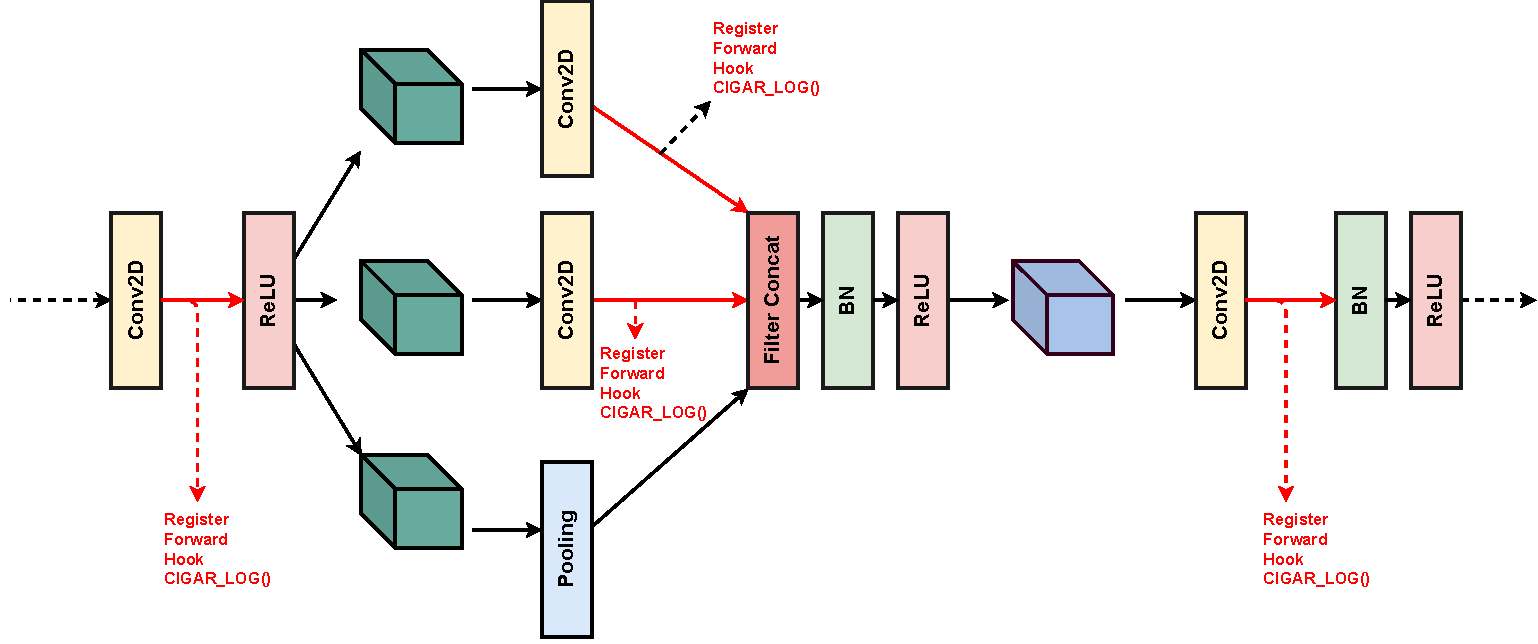
\includegraphics[scale=0.5]{fig/CIGAR.pdf}
    \caption{\ac{CIGAR} attachment of forward hooks to all model convolution layers}
    \label{fig:cigar_extraction}
\end{figure}

After all forward hooks are attached to the model, a forward pass of the model
is performed. Model layer statistics are added to the $model^{stats}_{dict}$ and
the collector's internal layer statistics tracker is reset. The layer statistics
collected are 1) the kernel sizes 2) strides 3) any additional padding 4)
input/output tensor dimensionalities 5) the number of convolution groups. After
processing all of the models in $model_{dict}$, a $model^{stats}_{dict}$ is
returned for further analysis used to derive the necessary library insights for
pruning the dataflow design space. An illustration of that process is available
in \autoref{fig:cigar_flow}. New layers can be analysed by CIGAR provided that the
collector is updated to be able to collect statistics from different layer types
and Attach\_Collection\_Hooks is allowed to attach the collector's callback
function to the newly supported layer. 

\begin{figure}
    \centering
    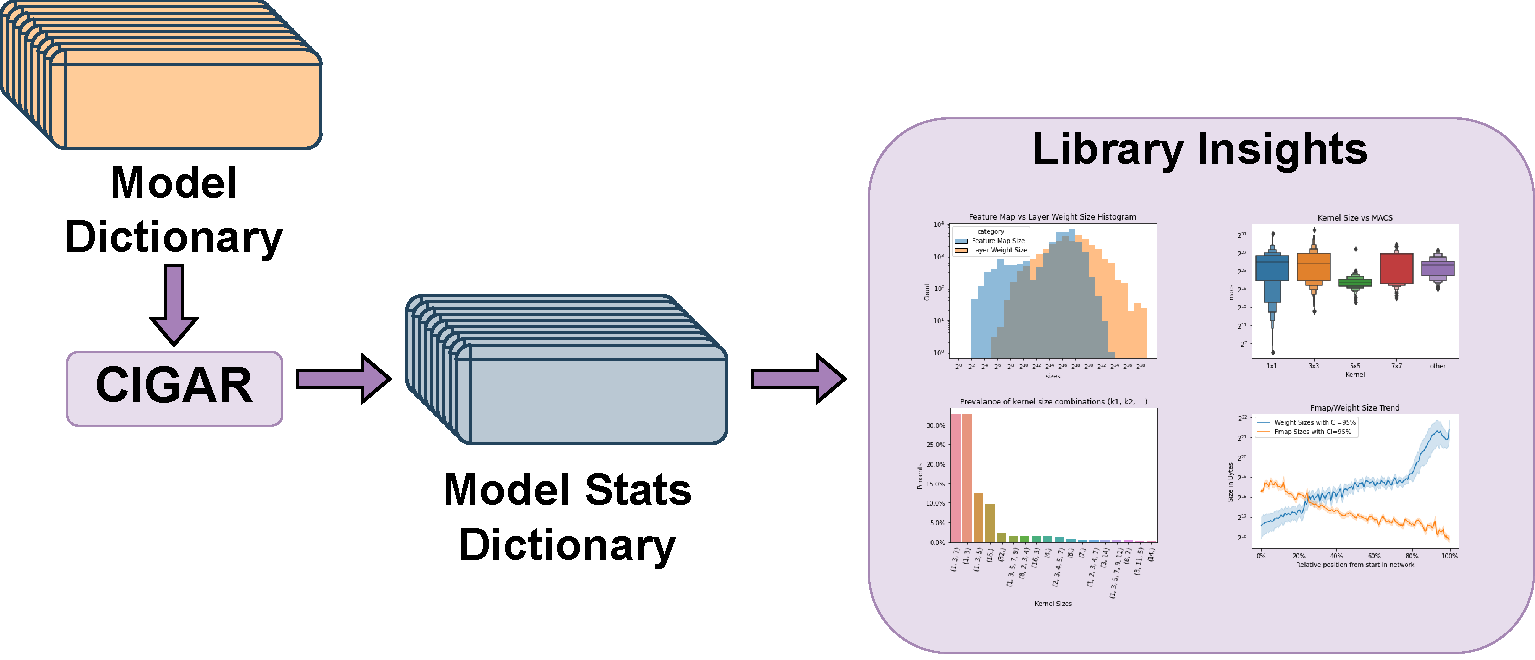
\includegraphics[scale=0.4]{fig/Cigar_flow.pdf}
    \caption{\ac{CIGAR} extraction of convolution layers}
    \label{fig:cigar_flow}
\end{figure}

\begin{algorithm}[H] 
    \caption{\ac{CIGAR}}
    \label{alg:cigar_algo}
    \begin{algorithmic}[1]
    \Require{$model_{dict}$} 
    \Ensure{$model^{stats}_{dict}$}
    \Statex
    \Function{Attach\_Collection\_Hooks}{$model, collector$}
        \State $hooks \gets []$
        \For{$layer \in model.named\_modules()$}
            \If{$type(layer)$ is $conv2d$} 
                \State $hooks.push(layer.register\_forward\_hook(collector.layer\_collector))$
            \EndIf 
        \EndFor
    \State \Return{$hooks$}    
    \EndFunction
    \Statex
    \Function{Collect\_Library\_Statistics}{$model_{dict}$}
        \State $model^{stats}_{dict} \gets \{\}$
        \State $collector \gets Collector()$
        \For{$(model_{name}, model) \in model_{dict}$}
            \State $input\_img\_tensor \gets transform(open('default.jpg'), model)$
            \State $hooks \gets Attach\_Collection\_Hooks(model, collector)$
            \State $model.forward(input)$
            \State $model^{stats}_{dict}[model_{name}] \gets collector.model\_stats()$
            \State $collector.reset()$
            \State $hooks \gets Detach\_Collection\_Hooks(hooks)$
        \EndFor
        \State \Return {$model^{stats}_{dict}$}
    \EndFunction
    \end{algorithmic}
\end{algorithm}

\subsubsection{Neural Network Library Explored}
\label{chap:dataflow_dse:pruning:cigar:library}

A diverse range of networks were explored by CIGAR for dataflow design space
pruning. The diversity of networks is reflected in the diversity of model types,
layer types, model sizes, and the number of MACs in the network. An illustration
of the model sizes vs number of MAC diversity is presented in
\autoref{fig:cigar_library_overview}. From \autoref{fig:cigar_library_overview}
it is clear that a wide range of models were selected as part of the CIGAR
library explored. The library includes smaller models like squeezenet and
mobilenetv2 as well as larger models like VGG16 \cite{dnn_is_sota_image}.
Additionally, in addition to image recognition networks, the library includes
object detection networks like yolov5 \cite{DBLP:journals/corr/abs-2108-11539}.
In terms of layer diversity the library includes conventional networks with both
convolution layers and linear layers as well as newer more exotic networks that
combine tranformer self attention layers with convolution layers like CoAtNet
\cite{xu_co-scale_2021}. An illustration of that layer type diversity is
reflected in figure \autoref{fig:cigar_library_overview}.b. A total of 63 base networks where explored, of which there
are 419 variants. The full list of networks explored is available in the
appendix of this thesis. All models explored by CIGAR were implemented in
pytorch and provided by either torchhub in \cite{pytorch} or the PyTorch Image
Models (timm) package in \cite{timm}.  

\begin{figure}
    \centering
    \subfigure[]{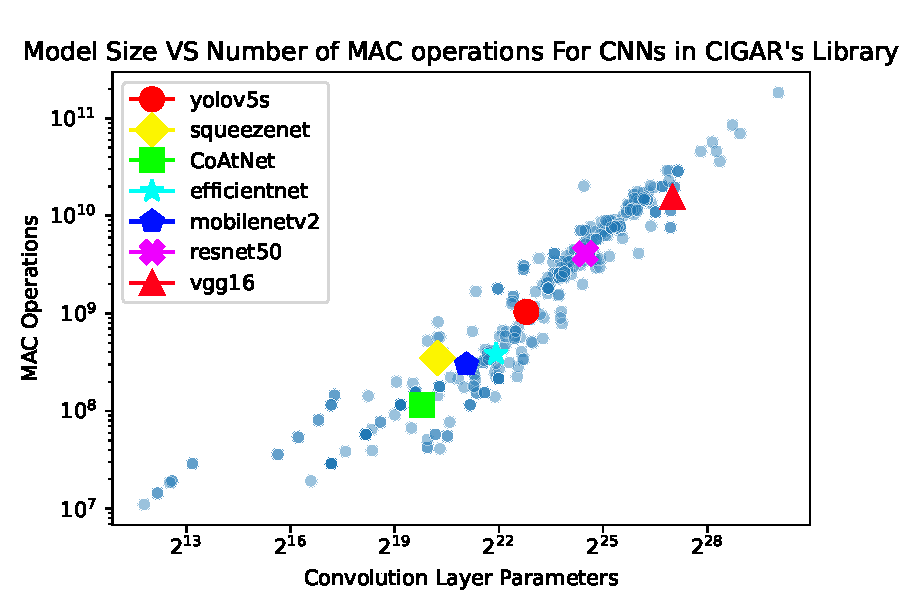
\includegraphics[width=0.495\textwidth]{Plots/CIGAR_Library_Overview.pdf}}
    \subfigure[]{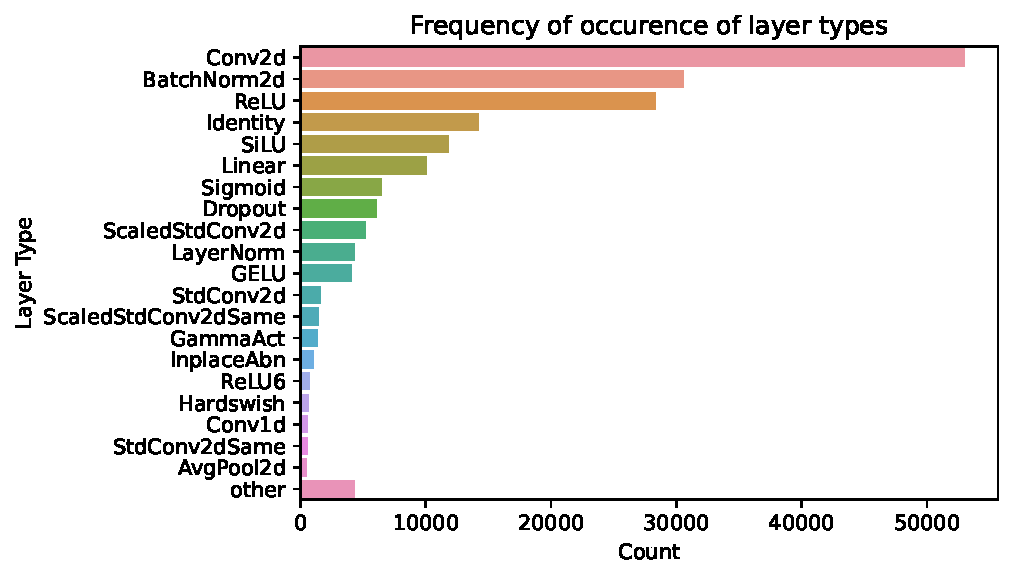
\includegraphics[width=0.495\textwidth]{Plots/layer_types_freq.pdf}}
    \caption{Illustration of CIGAR's library diversity based on (a) Model sizes and number of MACS (b) Model layer types}
    \label{fig:cigar_library_overview}
\end{figure}

\clearpage

\subsection{Applying CIGAR to prune the dataflow design space}
\label{chap:dataflow_dse:pruning:applying_it}

\subsubsection{Loop Unroll Targets}
\label{chap:dataflow_dse:pruning:applying_it:loop_unroll_targets}

\begin{figure}
    \centering
    \subfigure[]{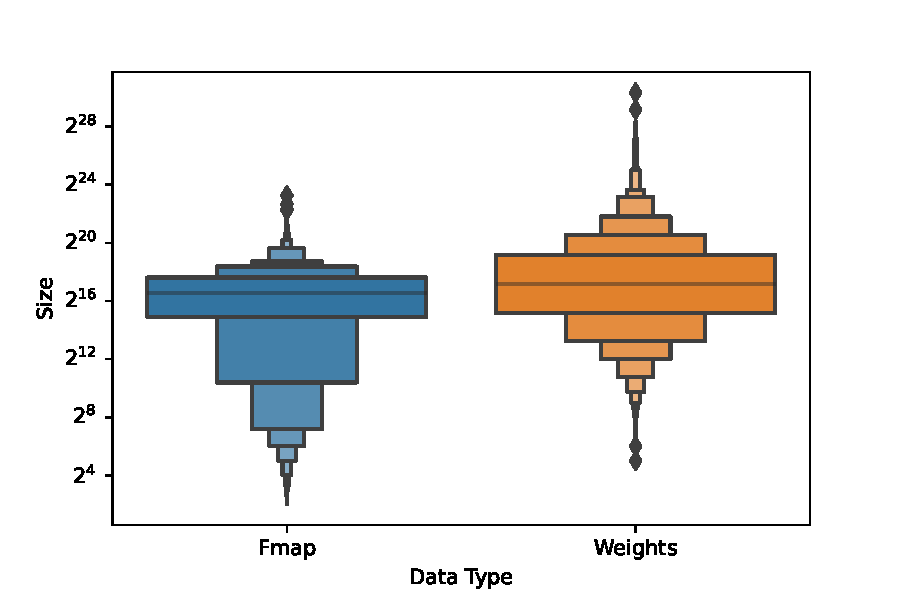
\includegraphics[width=0.495\textwidth]{Plots/WeightVsFmap_hist_no_lowering.pdf}}
    \subfigure[]{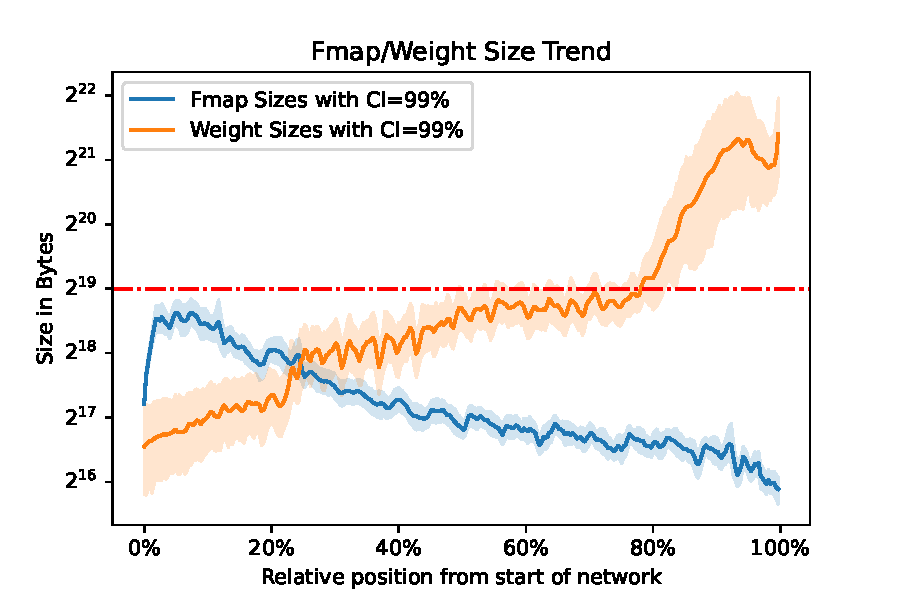
\includegraphics[width=0.495\textwidth]{Plots/fmap_size_trends_no_lowering.pdf}}
    \caption{Exploration of Feature map vs Weights sizing statistics a) in entire CIGAR library b) as trends within networks}
    \label{fig:fmap_vs_weight_hist}
\end{figure}



After running CIGAR on the model library referenced in
\autoref{chap:dataflow_dse:pruning:cigar:algo} the aggregate library statistics
show that there exists a discrepancy in layer feature map sizing vs layer weight
sizing as seen in \autoref{fig:fmap_vs_weight_hist}. While both data types share
similair median sizes at ~$2^{17}$ (assuming 8 bit precision for both), for 95\%
of layers, IFmap sizes fell below $2^{19.11}$ bytes, but for 95\% of layers
weights, weight sizes falls below $2^{22.17}$ bytes. This descripency in sizing
suggests that a weight stationary dataflow involving the loop unroll targets F,
C, KY, and KX might be appropriate given that it maximizes on-chip reuse of
weights and minimizes expensive reloads of weights from DRAM. A reduction of
DRAM activity generally leads to better energy efficiency during processing of a
convolution layer. Additionally, due to the overlap between 1x1 convolutions and
GEMM discussed in \autoref{chap:conv_gemm_equiv}, the choice of a weight
stationary dataflow lends itself well to \ac{GEMM} given the similarities in the
loop structure with regards to F and C loops for both applciations. Furthermore,
a weight stationary based dataflow allows support for linear layers which are
quite prevelant in many moder networks as seen in
\autoref{fig:cigar_library_overview}.b.

\clearpage
\begin{lstlisting}[language=C, caption=Weight stationary dataflow, label={lst:conv_loop}]
#pragma UNROLL F_UNROLL
for(int f = 0; f < F; f+=F_UNROLL) // Filter loop
#pragma UNROLL C_UNROLL
    for(int c = 0; c < C; c+=C_UNROLL) // Channel loop
        for(int y = 0; y < Y; y+=1) // Output feature map row
            for(int x = 0; x < X; x+=1)  // Output feature map col
#pragma UNROLL KY_UNROLL
                for(int ky = 0; ky < KY; ky+=KY_UNROLL)  // Kernel row
#pragma UNROLL KX_UNROLL
                    for(int kx = 0; kx < KX; kx+=KX_UNROLL)  // Kernel col
                        O[f][y][x] += I[c][y+ky][x+kx]*W[f][c][ky][kx];
\end{lstlisting}

\begin{lstlisting}[language=C, caption=GEMM loops, label={lst:W_S_Generic_Loop}]
    #pragma unroll F_UNROLL
    for(int f = 0; f < F; f+=F_UNROLL) // Filter loop
    #pragma unroll C_UNROLL
        for(int c = 0; c < C; c+=C_UNROLL) // Channel loop
            for(int z = 0; z < Z; z+=1)
                O[f][z] += W[f][z]*I[c][z];
\end{lstlisting}

\subsubsection{Loop Unroll Factors}
\label{chap:dataflow_dse:pruning:applying_it:loop_unroll_factors}

There exists significant variation with regards to the kernel sizes present in
CIGAR's library. This makes the question of unroll factors and axis mapping for
the KY and KX loops more difficult.

From \autoref{fig:kernel_sizes}.a 1x1 and 3x3 kernel sizes dominate in
comparison to all other kernel sizes. This renders the choice of keeping KY and
KX loops folded impractical because if support is extended to an arbitrary K x K
kernel while KY and KX loops are folded the onboard storage for weights would
then need to be at least $K^2$ where $K$ is the upperbound of kernels supported
directly to avoid excessive weight fetches from DRAM. Unfortunatly, for ~60\% of
the layers in the network, that additional storage area would be significantly
underutilized by a factor of $\frac{1}{K^2}$ due to the overrepresentation of
1x1 kernels. To mitigate this underutilization of onboard memory for weights, KY
and KX loops need to be unrolled fully. However, this begs the question, what
kernel sizes should be assumed when unrolling the KY and KX loops? Any kernel
sizes assumed when unrolling KY and KX loops become kernel sizes that are
supported directly. Kernel sizes that are not assumed when unrolling KY and KX
loops can be supported indirectly through the approach outlined in
\autoref{chap:conv_gemm_equiv}. This means that 1x1 kernels are assumed when
unrolling KY and KX loops, hence they are by definition supported directly.
Other kernel sizes to support directly can be derived from
\autoref{fig:kernel_sizes}. 

In \autoref{fig:kernel_sizes}.b many networks contain at least 1 convolution
layer that is not 1x1 or 3x3. For example a 7x7 kernel exists in around ~37\% of
networks. The reason for the prevalance of 7x7 convolutions originates from the
historical use of resnet \cite{resnet} as a feature extractor for a significant
portion of networks analyzed by CIGAR. In \autoref{fig:kernel_sizes}.c, when
adjusting for the the number of MACs present in layers where these kernel sizes
exist, 1x1 and 3x3 kernels share a similar computational burden on the network
with 1x1 having a much wider spread. 7x7 kernels have a much tighter spread but
they still represent a similar computational burden to 3x3 kernels in networks
where they are present. In \autoref{fig:kernel_sizes}.d we can see that in
networks where non 1x1 and 3x3 kernels exist, they are not likely to dominate
network layers which echo's the prevalance data in \autoref{fig:kernel_sizes}.a.
For example the median percentage of 7x7 and 5x5 layers in a network that has
them is 1.5\% and 11.1\% respectively.
From \autoref{fig:kernel_sizes} it is clear that 1x1 and 3x3 kernels need to be
supported directly while all other kernels need to be supported indirectly
through the approach in \autoref{chap:conv_gemm_equiv}. This limits the space of
possible unroll factors for the loop unroll targets and thus prunes the dataflow
design space. Supporting kernels indirectly will lead to an expansion of the
IFmap due to the duplication introduced by lowering, however that expansions is
negligble given the scarcity of non 1x1 and 3x3 layers. Applying lowering to
unsupported layers increases the required storage for IFmap due to lowering from 
from $2^{19.11}$ to at most $2^{19.25}$ for 95\% of layers.

\clearpage
\begin{figure}
    % Todo: update figure titles to reflect origins of statistics
    \centering
    \subfigure[]{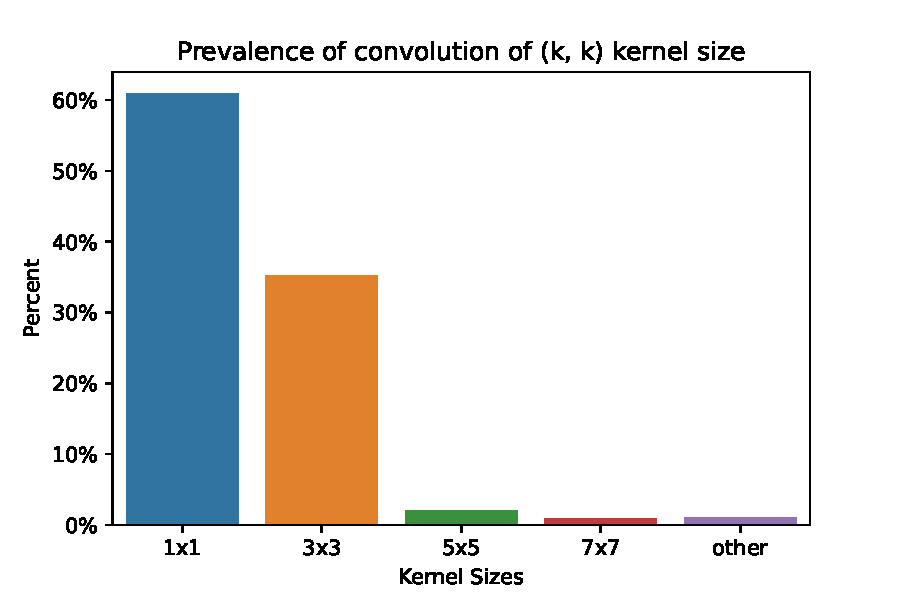
\includegraphics[width=0.495\textwidth]{Plots/kernel_size_prcnt.pdf}}
    \subfigure[]{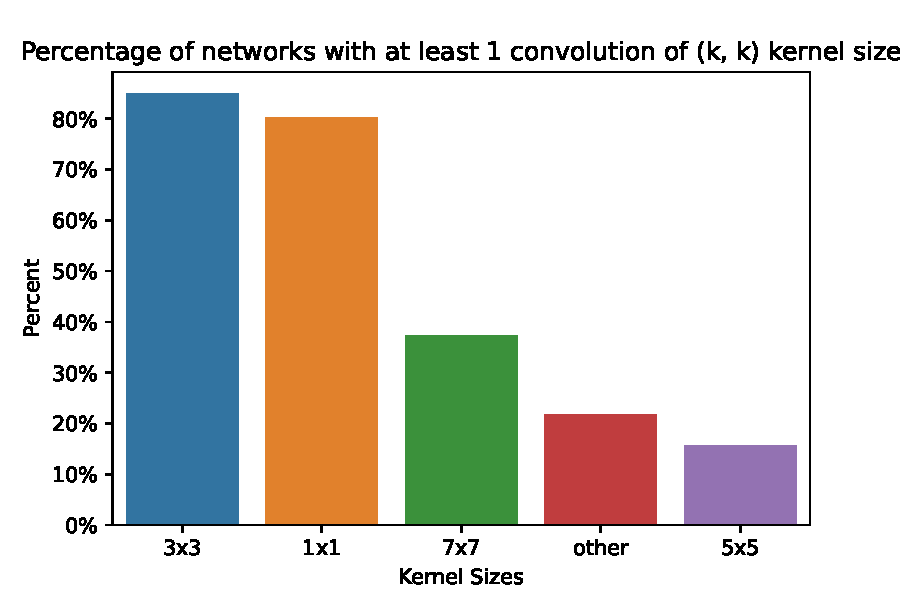
\includegraphics[width=0.495\textwidth]{Plots/kernel_size_atleast_once.pdf}}
    \subfigure[]{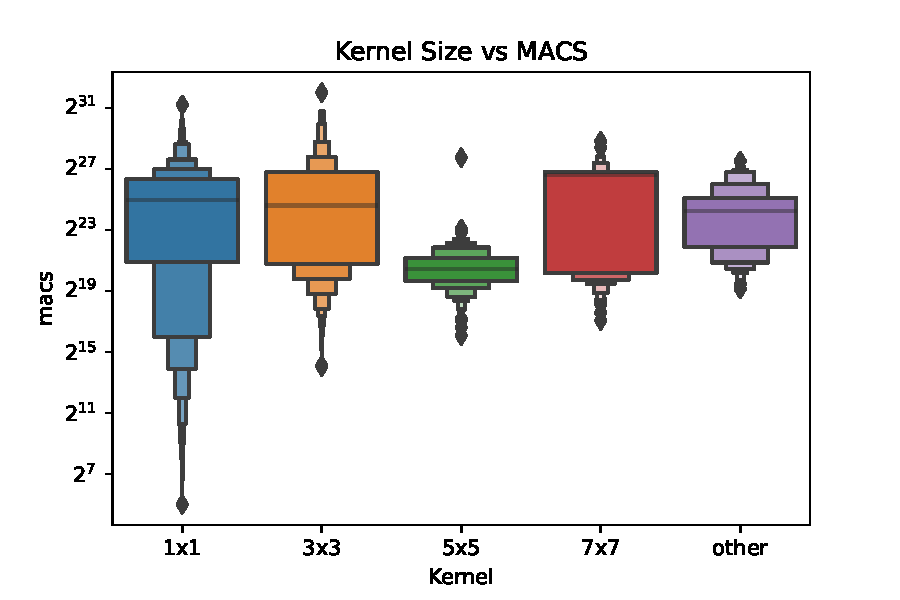
\includegraphics[width=0.495\textwidth]{Plots/Kernel_Size_vs_MACS.pdf}}
    \subfigure[]{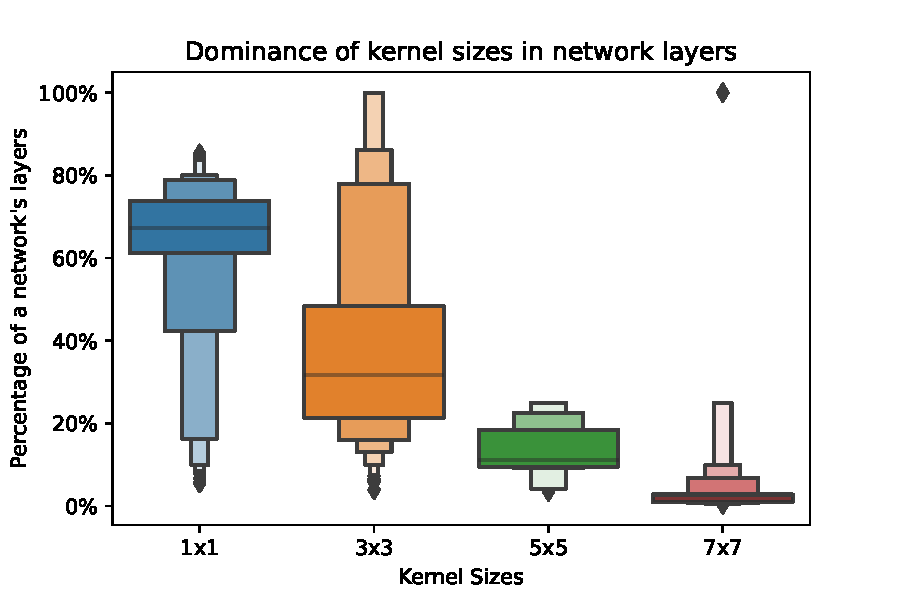
\includegraphics[width=0.495\textwidth]{Plots/kernel_dominance.pdf}}
    \caption{Feature map vs Weights sizing statistics in (a) Entire CIGAR library (b) For each convolution layer in the network}
    \label{fig:kernel_sizes}
\end{figure}

% TODO: Introduce tiling discussion here using tiling figure
Depending on the chosen unroll factors, the architecture implementing the unroll
factors in effect tiles the weight tensor and processes it tile by tile in the
convolution operation. An
illustration of this concept is present in
\autoref{fig:tiling_connection_to_unroll_targets}. Loop unroll factors determine
PE allocation 
Tiling of a weight tensor arises from the processing of filters, channels and
kernels in chunks whose size depend on the unroll factors. 
Padding of a weight tensors is performed wherever the chosen PE
binding for filter or channel loops exceeds the number of channels and filters
being processed in the tile. In
\autoref{fig:tiling_connection_to_unroll_targets} a weight tensors of dimension
$R^{6\times 3\times 2\times 2}$ is tiled with $F_{unroll} = 4$, $C_{unroll}=8$,
$K_{unroll}=2$ with kernel loops mapped to the horizontal axis alongside channel
loops. Additional padding in the horizontal and verticle axis is added given
excess allocation of PEs in both spatial axis in all tiles except the top left
one. This representation of the weight tensor as a series of tiles processed by
the architecture is useful when considering different schedules for processing
weights. A discussion of tile scheduling is given in the next section. 

\begin{figure}[]
    \centering
    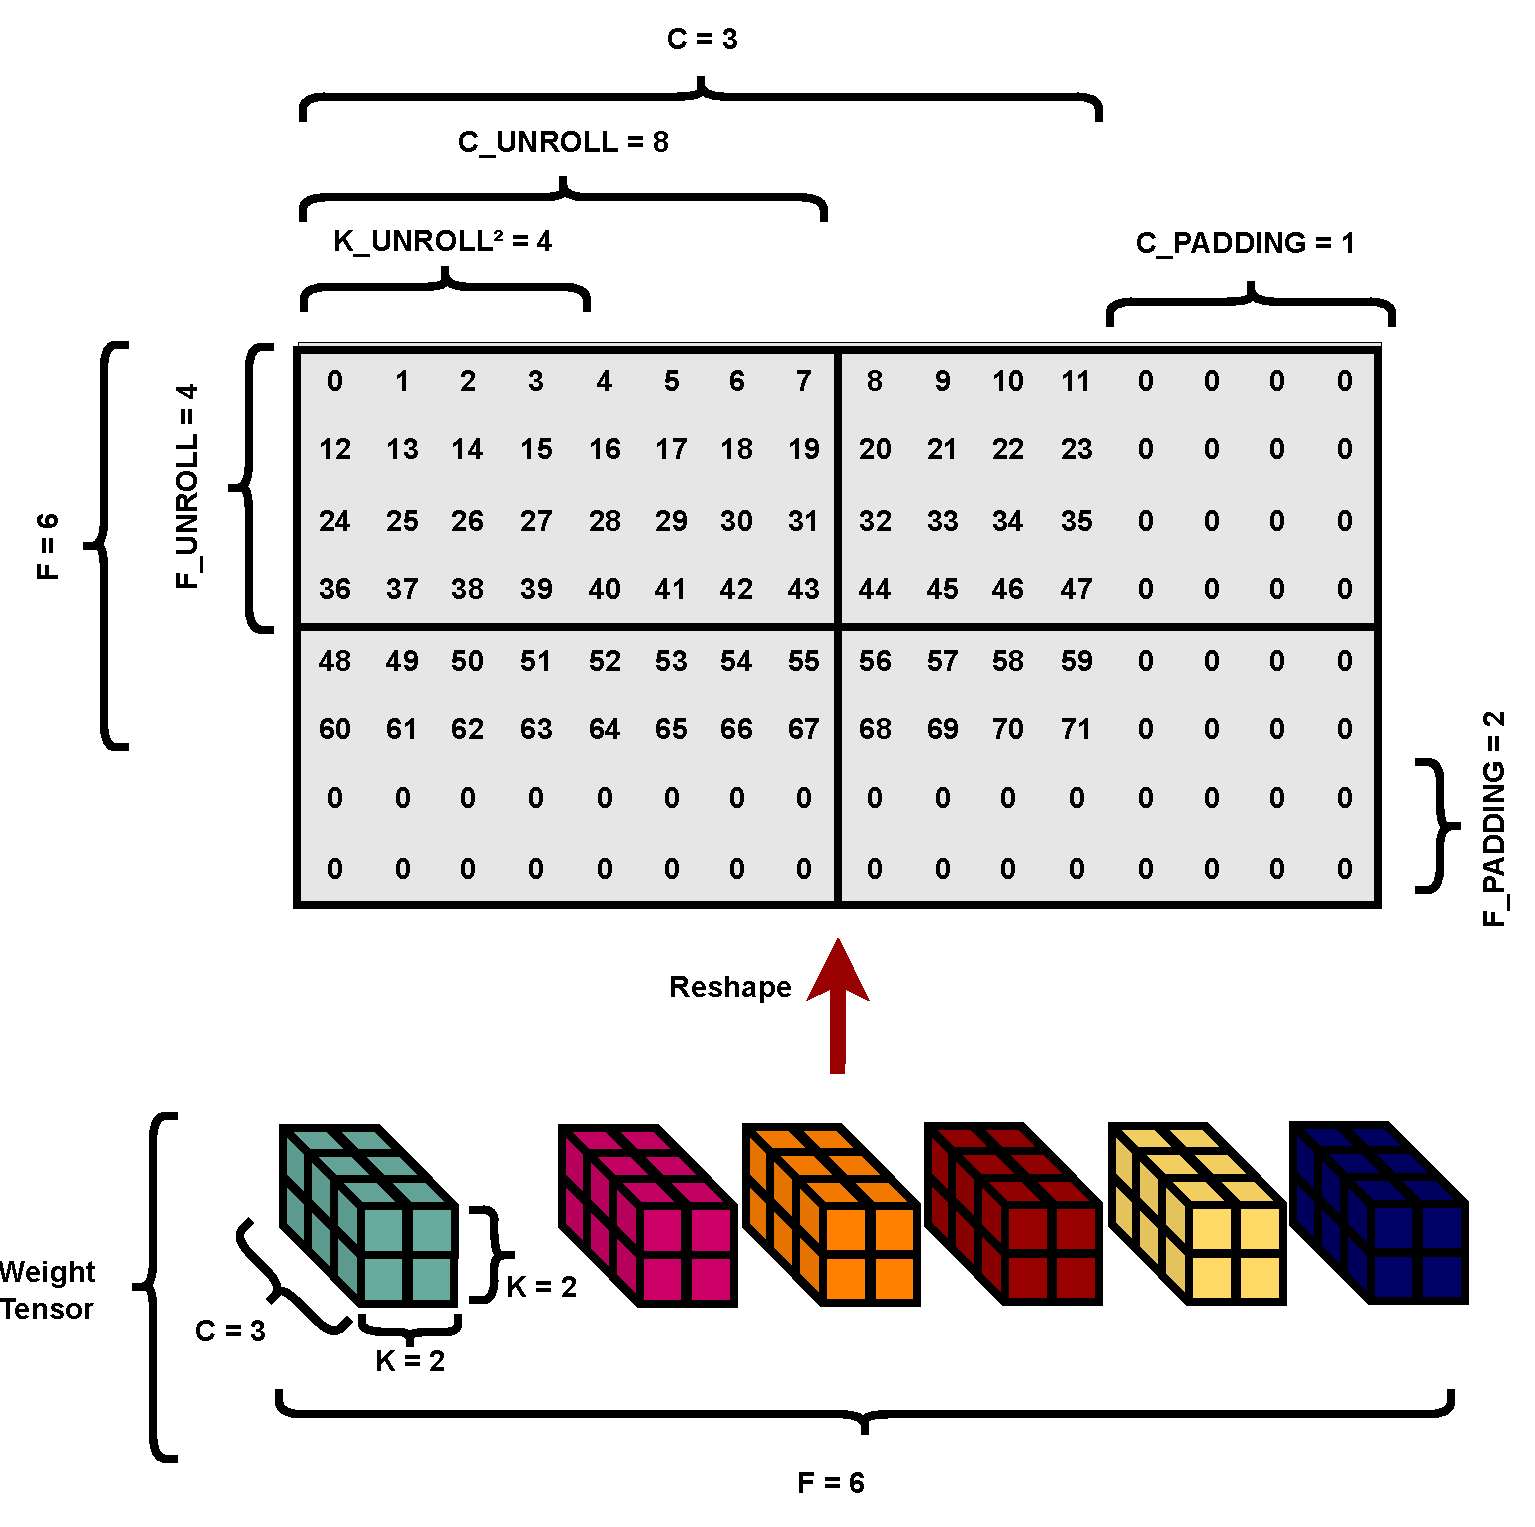
\includegraphics[scale=0.5]{fig/tiling.pdf}
    \caption{\ac{GEMM} and 1x1 Convolution Equivelence}
    \label{fig:tiling_connection_to_unroll_targets}
\end{figure}

\clearpage 

\subsubsection{Loop ReOrdering}
\label{chap:dataflow_dse:pruning:applying_it:loop_ordering}

% In the final template there are 4 template parameters that are customizable
% depending on the target performance/area/energy efficiency requirements of the
% acclerator. The first and the second are the unroll factors for filters
% ($F_{unroll}$) and channels ($C_{unroll}$). The third is the set of directly
% supported kernels. Finally the fourth is the spatial axis mapping of the kernel
% loops ($K_{axis}$). Each of these parameters has an effect on on-chip storage
% required for the different memories accessed.

\begin{figure}
    \centering
    \subfigure[]{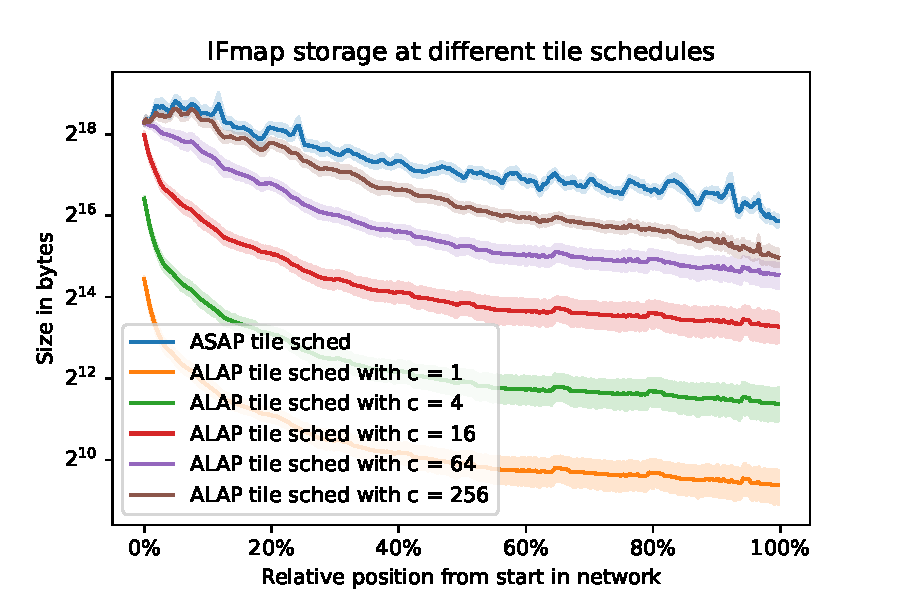
\includegraphics[width=0.45\textwidth]{Plots/ifmap_Storage.pdf}}
    \hspace{0.1cm} 
    \subfigure[]{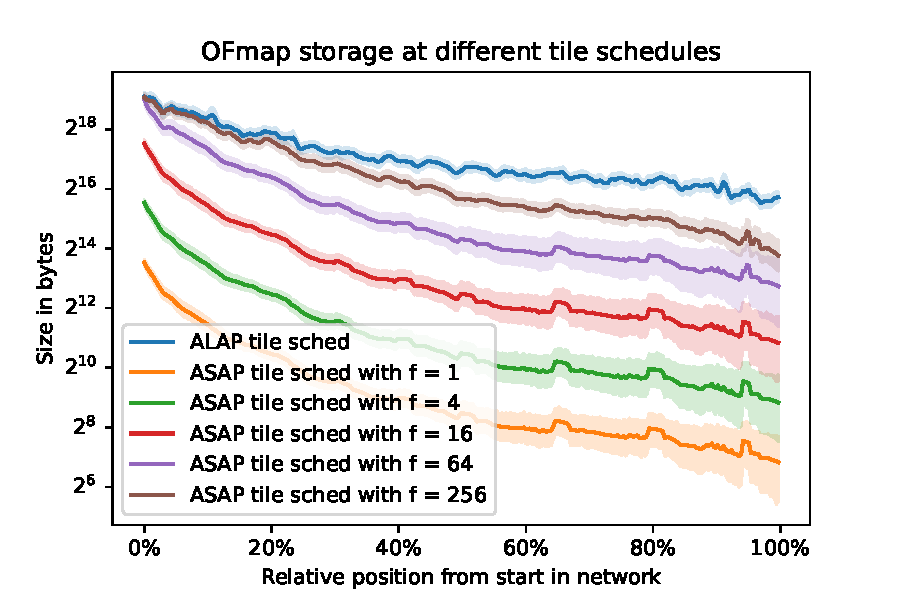
\includegraphics[width=0.45\textwidth]{Plots/PSUM_Storage.pdf}}
    \subfigure[]{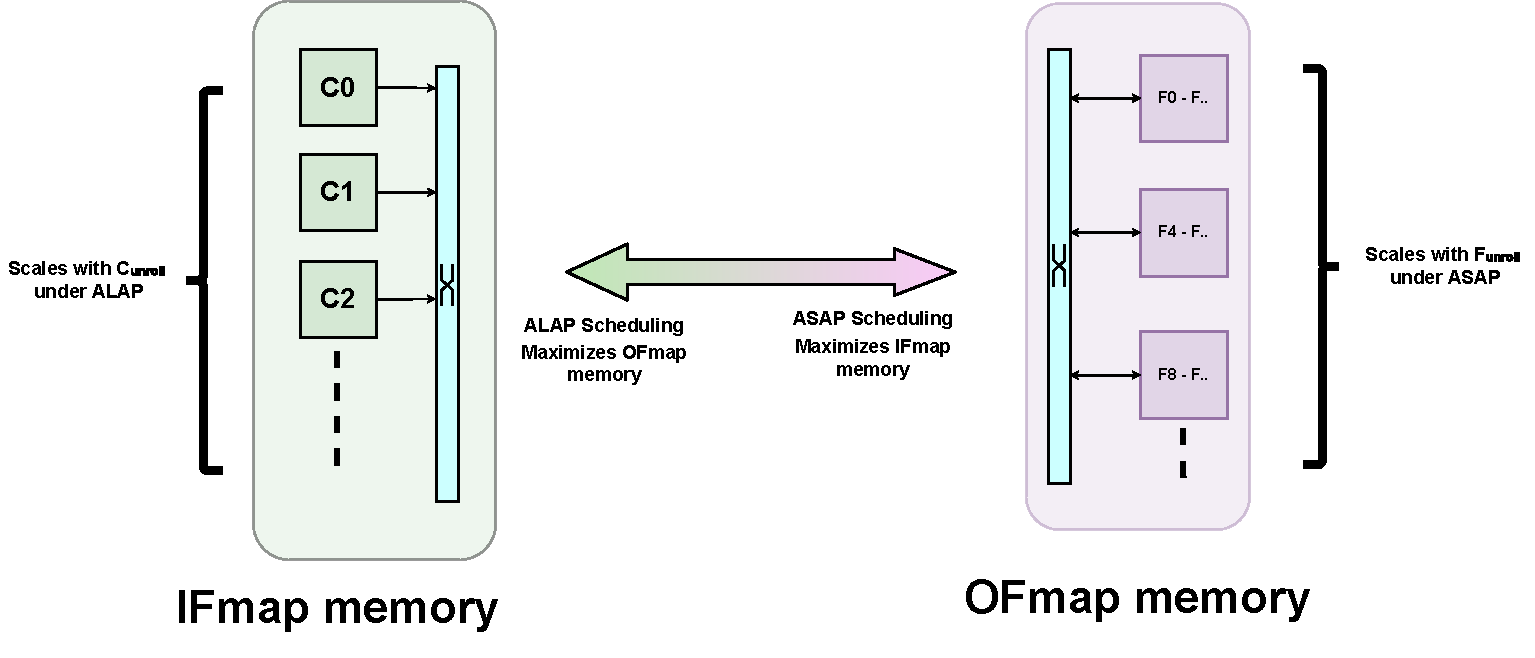
\includegraphics[width=1\textwidth]{fig/psum_ifmap_mem_scaling.pdf}}
    \caption{Illustration of storage tradeoff between OFmaps and IFmaps depending on tile scheduling (loop ordering) and accelerator template parameters (loop unroll factors) (a) IFmap storage (b) OFmap storage (c) archictural illustration}
    \label{fig:Fmap_scaling}
\end{figure}

\begin{figure}
    \centering
    \subfigure[]{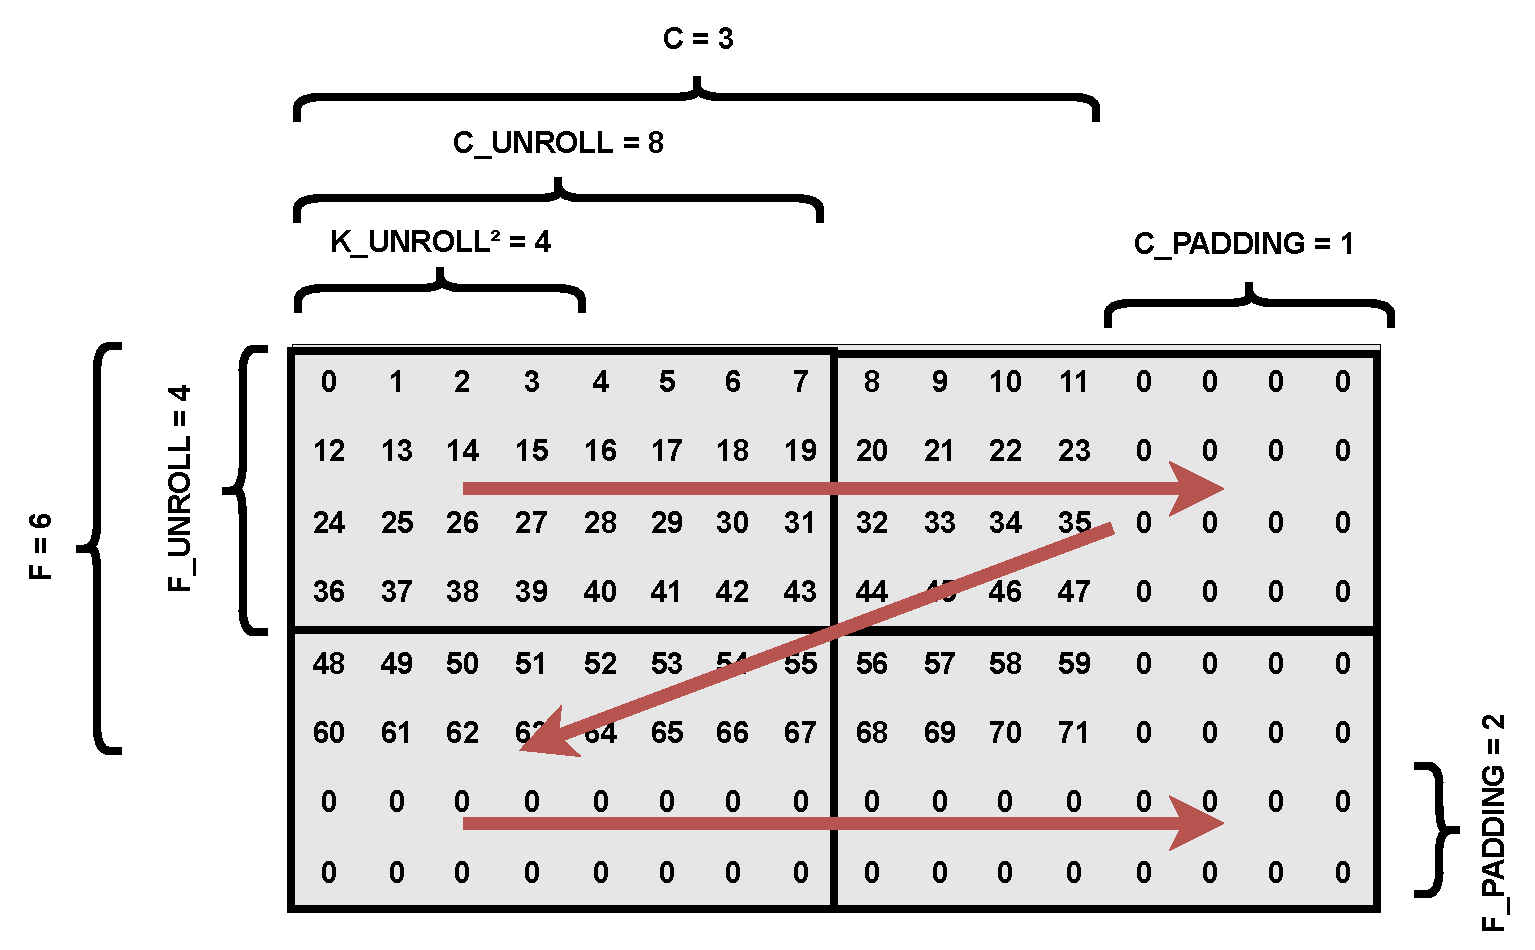
\includegraphics[width=1\textwidth]{fig/asap_tiling.pdf}}
    \hspace{0.1cm} 
    \subfigure[]{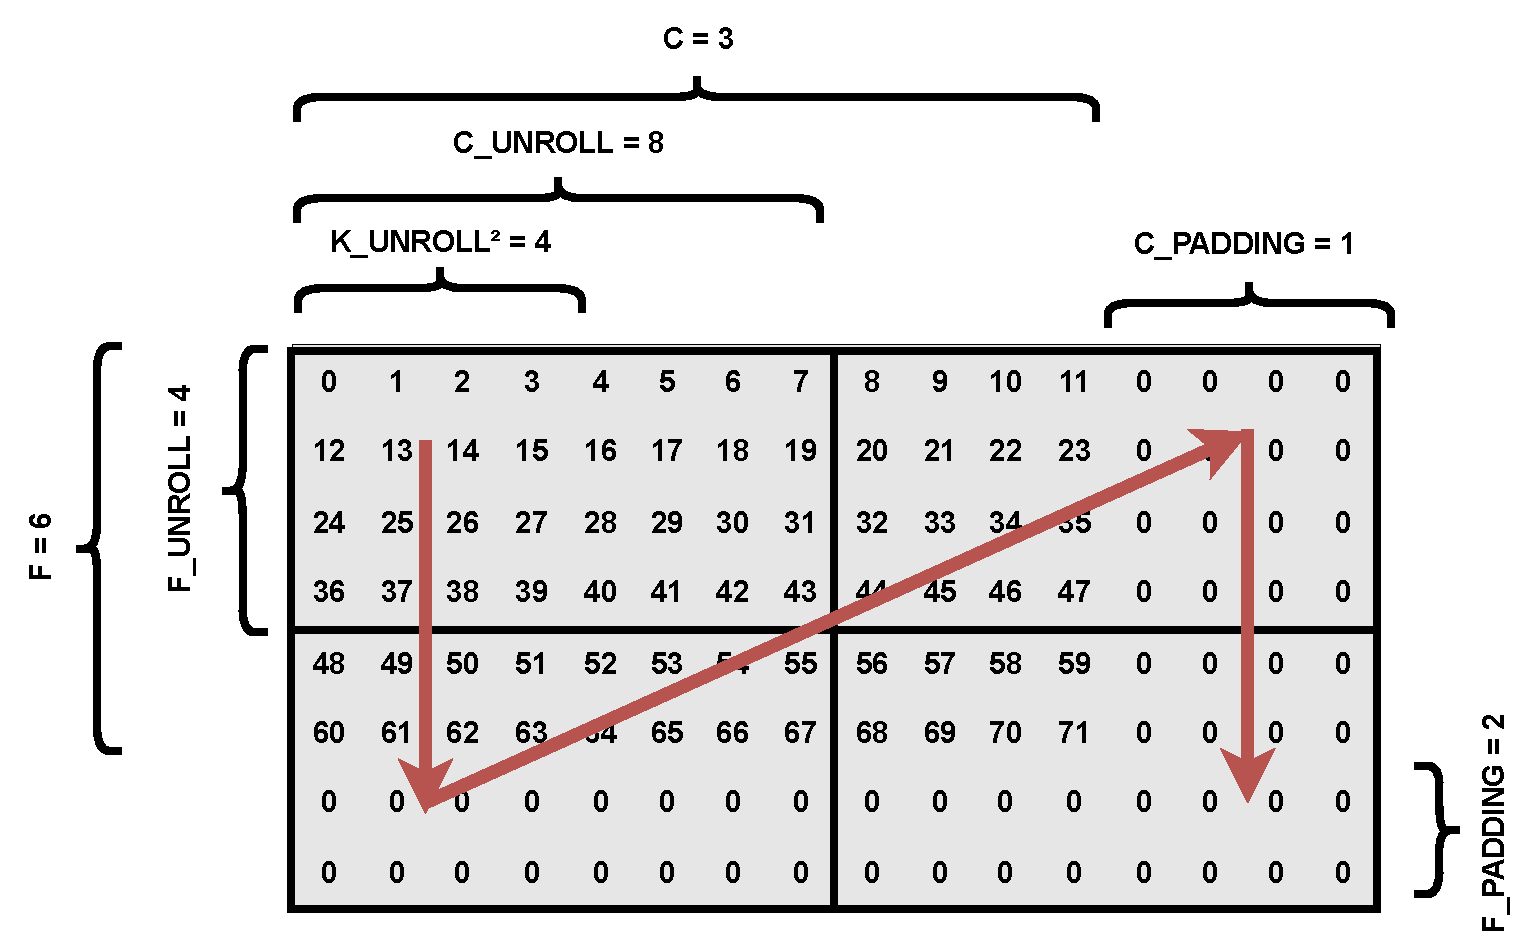
\includegraphics[width=1\textwidth]{fig/alap_tiling.pdf}}
    \caption{Illustration of different tiling schedules (a) ASAP scheduling (F, C)  (b) ALAP scheduling (C, F)}
    \label{fig:tile_scheduling}
\end{figure}


While a weight stationary offers limited flexibility with regards to loop
reoredering it does offer some degree of flexibiltiy with regards to ordering
filter loops and channel loops. F, C loop ordering affects required on-chip
storage for IFmaps and OFmaps.
Under Direct mode and Gemm mode with balanced lowering, IFmap sizes
do not exceed $2^{19.25}$ bytes (assuming 8 bit precision) for 95\% of all
convolution layers in CIGAR's library. An estimation of the
on-chip area required to store IFmaps using the model presented in
\cite{area_model} yields a total on-chip area per sram bit stored equal to 0.013
$um^2$ which translates to $0.064 mm^2$ on-chip area dedicated to sram buffers
for storing entire input feature maps for a layer at 14nm technology.
This area/storage does not scale with increased/decreased filter unroll factor,
channel unroll factor or max directly supported kernel size. On-Chip area
dedicated to storing Weights scales with the afformentioned parameters.
Storage with regards to OFmaps depends on the loop ordering in the chosen
dataflow. Specifically on-chip OFmap storage depends on whether filter loops and
channel loops are reordered such that OFmaps are retired as fast as possible
(ASAP tile scheduling) by iterating through IFmap channels first while
processing a groups of filter, or as late as possible (ALAP tile scheduling) by
iterating through filters first while processing a group channels. These two
orderings for filter loops and channel loops represent different tile schedules
for processing convolution layers. An illustration of both tile scheduling
approaches is illustrated in \autoref{fig:tile_scheduling}. In
\autoref{fig:tile_scheduling} a 1x1 convolution layer's weights are shown with
the architecture's unroll factors overlayed on top. The overlay of the
architecture's unroll factor creates distinct weight tiles where componenets of
the OFmap are computed. The order of executing these weight tiles depends on the
chosen tile schedule. ASAP which represents F, C loop ordering and ALAP which
represents C, F loop ordering. 

A tradeoff between required IFmap storage and required OFmap storage is apparent
in \autoref{fig:fmap_size_trends}. Under ASAP scheduling, storage requirements for
OFmaps scales with $F_{unroll}$ because $F_{unroll}$ represents the maxmimum
number of filters in flight. Storage requirements for IFmaps is maximized under
ASAP because all channel data would need to be held on-chip assuming no
additional reads can be made from DRAM for IFmap channels. Under ALAP
scheduling, storage requirements for IFmap scale with $C_unroll$ because
$C_{unroll}$ represents the maximum number of channels in flight. Storage for
OFmaps is maximized under ALAP. In this thesis it is assumed that chip
area (and thus on-chip memory) is always sufficient at least one of the
afformentioned tile schedules without requiring loop blocking and additional
DRAM accesses for feature maps. An exploration of the effect of loop blocking
under more restrictive area constraints is relegated to future work. 

\clearpage

\section{Hardware Implementation design space exploration with the Polyhedral Model}
\label{chap:hw_dse:intro}

Based on the conclusion derived from \autoref{chap:dataflow_dse:intro},
the ideal conv. accelerator operates in two modes, direct Mode where 3x3 kernel
with stride 1 are supported and GEMM mode where all other kernel sizes and
strides are supported in GEMM mode via the approach in (REFERENCE LOWERING/
LIFTING CHAPTER). In this section we will deduce the optimal hardware
implementation for the weight stationary dataflow chosen in
\autoref{chap:dataflow_dse:intro} by analyzing data reuse in the loop based
representation of the aforementioned dataflow. To perform this deduction we will
use the polyhedral model to analyse temporal reuse in
\autoref{chap:hw_dse:temporal_analysis} and spatial reuse in
\autoref{chap:hw_dse:spatial_reuse_analysis}. Finally, in
\autoref{chap:hw_dse:simplifying_hierarchy} a simplification of the IFmap memory
hierarchy present in the optimal hardware implementation derived in
\autoref{chap:hw_dse:temporal_analysis} and
\autoref{chap:hw_dse:spatial_reuse_analysis} is presented.

\subsection{Temporal Reuse Analysis}
\label{chap:hw_dse:temporal_analysis}

Unrolling convolution dataflow loops yield multiple instances of the \ac{MAC}
statement present in the original convolution nested loops in
\autoref{lst:conv_loop}. These instances will be referred to as \ac{MAC} spatial
instances to distinguish them from temporal instances discussed in this chapter.
\ac{MAC} spatial instances can be distinguished based on the memory access
offsets that exist in them as a result of unrolling filter, channel and kernel
loops. For unroll factors F\_T for filters, C\_T for channels, KY\_T and KX\_T
for kernels each statement will have a coresponding access offset based on the
spatial instance index $j \in [0, F\_T*C\_T*KY\_T*KX\_T]$ for each of the data
elements (IFmap, OFmap and Weights) accessed in the loop body. Each \ac{MAC}
spatial instance at index j is characterized by a set of access offsets {Fj, Cj,
KYj, KXj} used by the memory accesses in the \ac{MAC} statement. Applying the
unroll factors and distinguishing each \ac{MAC} statement based on it's
statement index j yields the loop configuration in
\autoref{lst:conv_loops_unrolled}. 

\begin{lstlisting}[language=C, caption=Fully unrolled convolution dataflow loops, label={lst:conv_loops_unrolled}]
    for(int f = 0; f < F; f+=F_T) // Filter loop
        for(int c = 0; c < C; c+=C_T) // Channel loop
            for (int y = 0; y < Y; y++) // FeatureMap Height
                for(int x = 0; x < X; x++) // FeatureMap Width
                        ...
                        /* For all j in [0, F_T*C_T*KY_T*KX_T[ */ 
                        O[f+Fj][y][x] += W[f+Fj][c+Cj][KYj][KXj]* \
                                            I[c][y+KYj][x+KXj] 
                        ...
\end{lstlisting}

Temporal reuse analysis is performed on the above loops. The different
operational modes (GEMM/ Direct) are analysed concurrently using the same loop
representation below as they only differ based on whether we fuse feature map
height and width loops, and set upper bounds of the kernel loops to 1. Since
kernel loops are always unrolled fully this sets KY\_T and KX\_T to 1. We can
analyse temporal reuse in the dataflow represented in
\autoref{lst:conv_loops_unrolled} by adapting the approach in \cite{meeus} 
to the afformentioned dataflow iteration domain and access functions.
Given iteration domain restrictions imposed by the polyhedral model,
\autoref{lst:poly:analysis} assumes unroll factors F\_T =
C\_T = 4. Setting F\_T and C\_T to concrete values does not affect output
results of temporal reuse analysis.

\clearpage
\begin{lstlisting}[caption=Polyhedral analysis of reuse in iscc for convolution loops, label={lst:poly:analysis}]
    // Define iteration domain for all accessed data elements
    ID:=[F, C, Y, X] -> { S[f, c, y, x] : 0<=f<F and 0<=c<C and f mod 4=0 and c mod 4=0, 0<=y<Y and 0<=x<X};
    // Define access functions for each data element
    IFMAP:=([Cj, KYj, KXj] -> {S[f, c, y, x] -> IF[c+Cj][y+KYj][x+KXj]})*ID;
    OFMAP:=([Fj] -> {S[f, c, y, x] -> PS[f+Fj][y][x]})*ID;
    WEIGHT:=([Fj, Cj, KYj, KXj] -> {S[f, c, y, x] -> W[f+Fj][c+Cj][KYj][KXj]})*ID;
    // Evaluate temporal reuse
    IFMAP_REUSE:=(IFMAP.(IFMAP^-1))*(ID<<ID);
    OFMAP_REUSE:=(OFMAP.(OFMAP^-1))*(ID<<ID);
    WEIGHT_REUSE:=(WEIGHT.(WEIGHT^-1))*(ID<<ID);  

\end{lstlisting}

In \autoref{lst:poly:analysis}, the iteration domain for the loops in
\autoref{lst:conv_loops_unrolled} is converted into it's set representation in
line 2 where for some access statement S the loop iteration vector [f, c, y, x,]
is bound by the upper and lower bounds [0, F], [0, C], [0, Y], [0, X]
respectively. These bounds are represented by the associated parameters passed
to the iteration domain set assignment in line 2. Each memory accessed in the
body of the loop has an access function at each level of that memory's
hierarchy. As a result, each instance of the loop iteration vector [f, c, y, x]
is mapped to a memory access for each of the memories in lines 4-6. Access
offsets used in the memory access functions are passed as parameters based on
the convention established in \autoref{lst:conv_loops_unrolled}. This mapping
creates multiple temporal instances for each memory access in each \ac{MAC}
spatial instance.  For
example, for some iteration vector [f = 1, c = 1, y = 0, x = 1],
 the OFmap access that occurs at iteration vector [f = 2, c= 1, y = 0,
x = 1] is a different temporal instance of the same OFmap access at [f = 1, c = 1,
y = 0, x = 1]. 
Two accesses that access the same index but at different
iteration vectors are different temporal instances of the same access.
After applying the operation in lines 8-10, we can determine the
temporal reuse behavior of the accessed memories in the convolution loops.  
\autoref{lst:poly:result} shows the reuse behavior for each memory. Original
iteration domains constraints are ommited for brevity. 

\clearpage
\begin{lstlisting}[caption=Polyhedral analysis results w.r.t data elements in convolution loops, label={lst:poly:result}]
    IFMAP_REUSE;
    [F, C, Y, X, Cj, KYj, KXj]->{
        S[f, c, y, x] -> S[f', c' = c, y' = y, x' = x] :
            ... f' > f and 0 <= f' < F ... 
        }
    OFMAP_REUSE;
    [F, C, Y, X, Fj]->{ 
        S[f, c, y, x] -> S[f' = f, c', y' = y, x' = x] : 
            ... c' > c and 0 <= c' < C ... 
        }
    WEIGHT_REUSE;
    [F, C, Y, X, Fj, Cj, KYj, KXj] -> { 
        S[f, c, y, x] -> S[f' = f, c' = c, y', x'] : 
            ... y' > y and 0 <= y' < Y and 0 <= x' < X ...; 
    }
\end{lstlisting}

\autoref{lst:poly:result} shows the temporal reuse behavior in memory accesses. For each
of the memories accessed (IFmap, OFmap and Weights) there exists a set of reuse
(IFMAP\_REUSE, OFMAP\_REUSE and WEIGHT\_REUSE) maps that map each iteration
vector of an access to all the proceeding iteration vectors where that same
access occurs. From the above listing we can see that, in the set of IFmap reuse
maps (IFMAP\_REUSE), IFmap channels are reused temporally with respect to filter
loops. For a given IFmap accessed at channel c, that channel is accessed again
when computing the output for all proceeding filter loop iterationtions f' where
$f'>f$. The absence of other mappings in the set of reuse maps IFMAP\_REUSE shows
that 1) this reuse behavior holds at any arbitrary iteration vector [f, c, y, x]
and 2) this reuse behavior depends only on the filter loop. For the set OFmap
reuse maps (OFMAP\_REUSE), for an OFmap acceess at iteration vector [f, c, y,
x], it is accessed again at loop iteration f'=f, c', y'=y, x'=x where $c'>c$.  
For (WEIGHT\_REUSE) Weights exhibit temporal reuse w.r.t feature map width and
height, the X and Y loops. 

Applying the hardware taxonomy in \cite{maestro}, IFmap exhibits temporal reuse,
multicast communication. OFmap exhibits temporal reuse, reduction communication
given their read-modify-write behavior. Weights exhibit temporal multicast
communication. Given the limited implementation options derivable from temporal
reuse we can comfortably define the appropriate connectivity and memory
hierarchies for IFmaps channels, OFmaps channels (equivelent to number of
Filters), and Weights. The beginings of a hardware template derived from the
afformentioned temporal reuse behavior of the different memories referenced in
the convolution dataflow can be seen in \ref{fig:reuse_illus}. In
\ref{fig:reuse_illus} the template is broken into 3 major componenets. The first
is the IFmap memory hierarchy currently with only 1 level. The 2nd component is
the compute portion of the template where partial sums are computed and
aggregating into OFmap data elements. Finally the 3rd component which is the
OFmap memory that stores OFmap partial sums until they are aggregated into OFmap
pixels and are written back to memory.

\begin{figure}[]
    \centering
    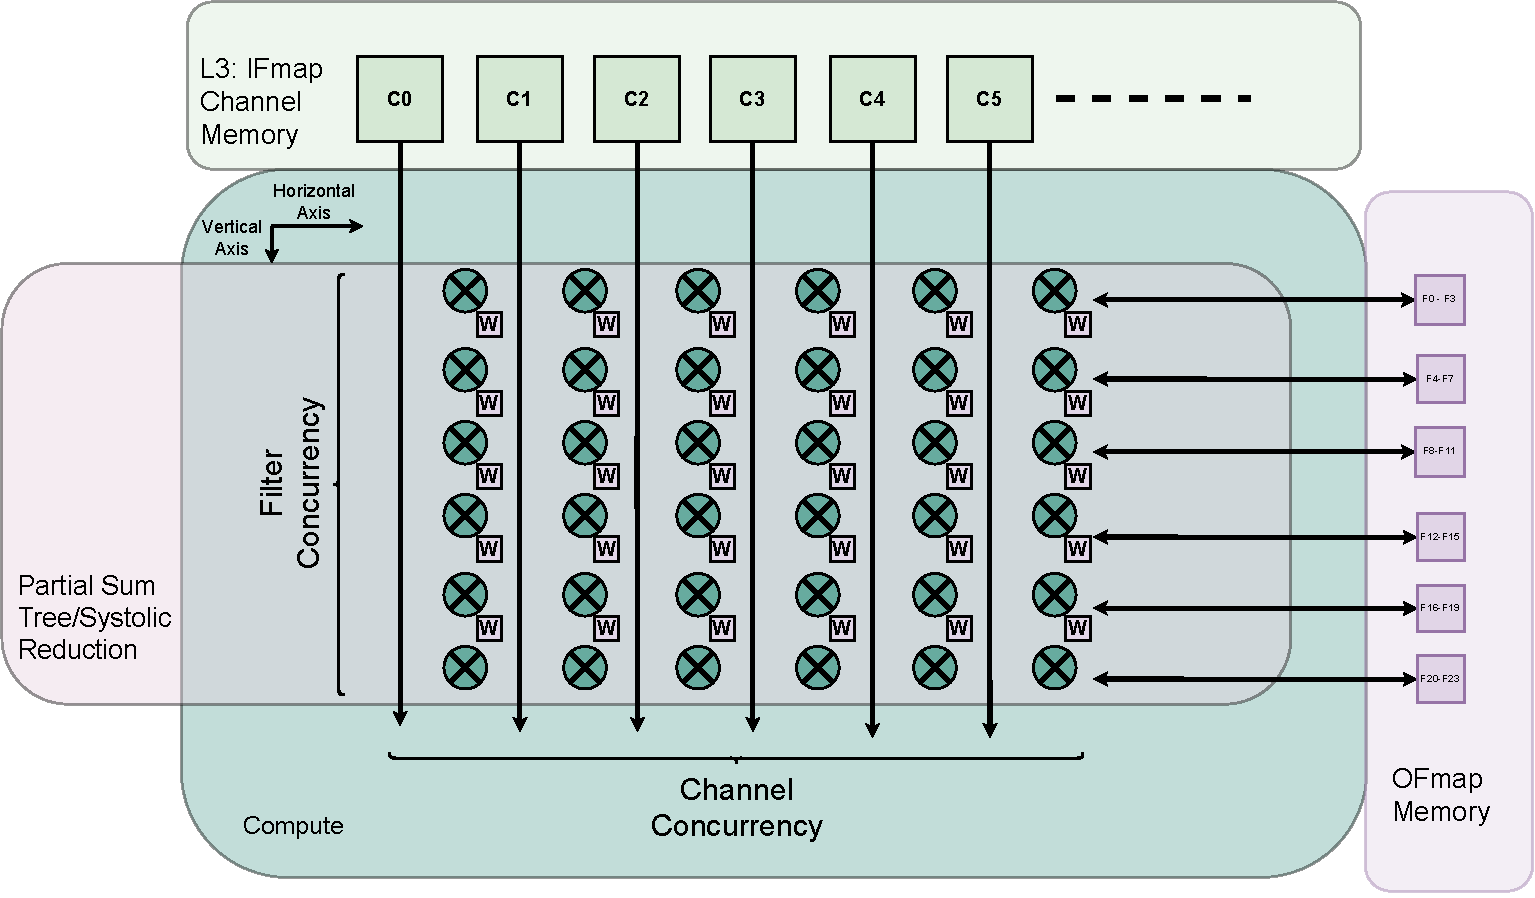
\includegraphics[scale=0.4]{fig/reuse_illus.pdf}
    \caption{Initial hardware template incorporating buffers IFmap and OFmap temporal reuse}
    \label{fig:reuse_illus}
\end{figure}

In addition to the temporal reuse behavior exhibited across IFmap channels,
temporal reuse exists within individual IFmap channels due to the stencil based
access pattern arising from the X, Y, KY, KX loops in the dataflow. That
temporal reuse is affected by the decision to fully unroll kernel loops which
causes temporal reuse to exist between unrolled IFmap kernel ports. Proof of the
existence of that temporal reuse is given in the polyhedral analysis in
\autoref{lst:poly:xy_reuse}. 

\begin{lstlisting}[caption=Analysis of IFmap channel reuse, label={lst:poly:xy_reuse}]
    ID_XY:=[Y, X, KY, KX] -> { S[y, x, ky, kx] : 0<=ky<KY and 0<=kx<KX and 0<=y<Y and 0<=x<X};
    IFMAP_XY:=({S[y, x, ky, kx] -> IF[y+ky][x+kx]})*ID;
    IFMAP_REUSE_XY:=(IFMAP_XY.(IFMAP_XY^-1))*(ID_XY<<ID_XY);
    IFMAP_XY_REUSE;
    [Y, X, KY, KX] -> { 
        S[y, x, ky, kx] -> S[y', x', ky' = (y - y') + ky, kx' = (x - x') + kx] : 
            ... y' > y and (y + ky) -KY < y' <= (y + ky) and (x + kx) -KX < x' <= (x + kx) ...;
    }
\end{lstlisting}

\begin{figure}[]
    \centering
    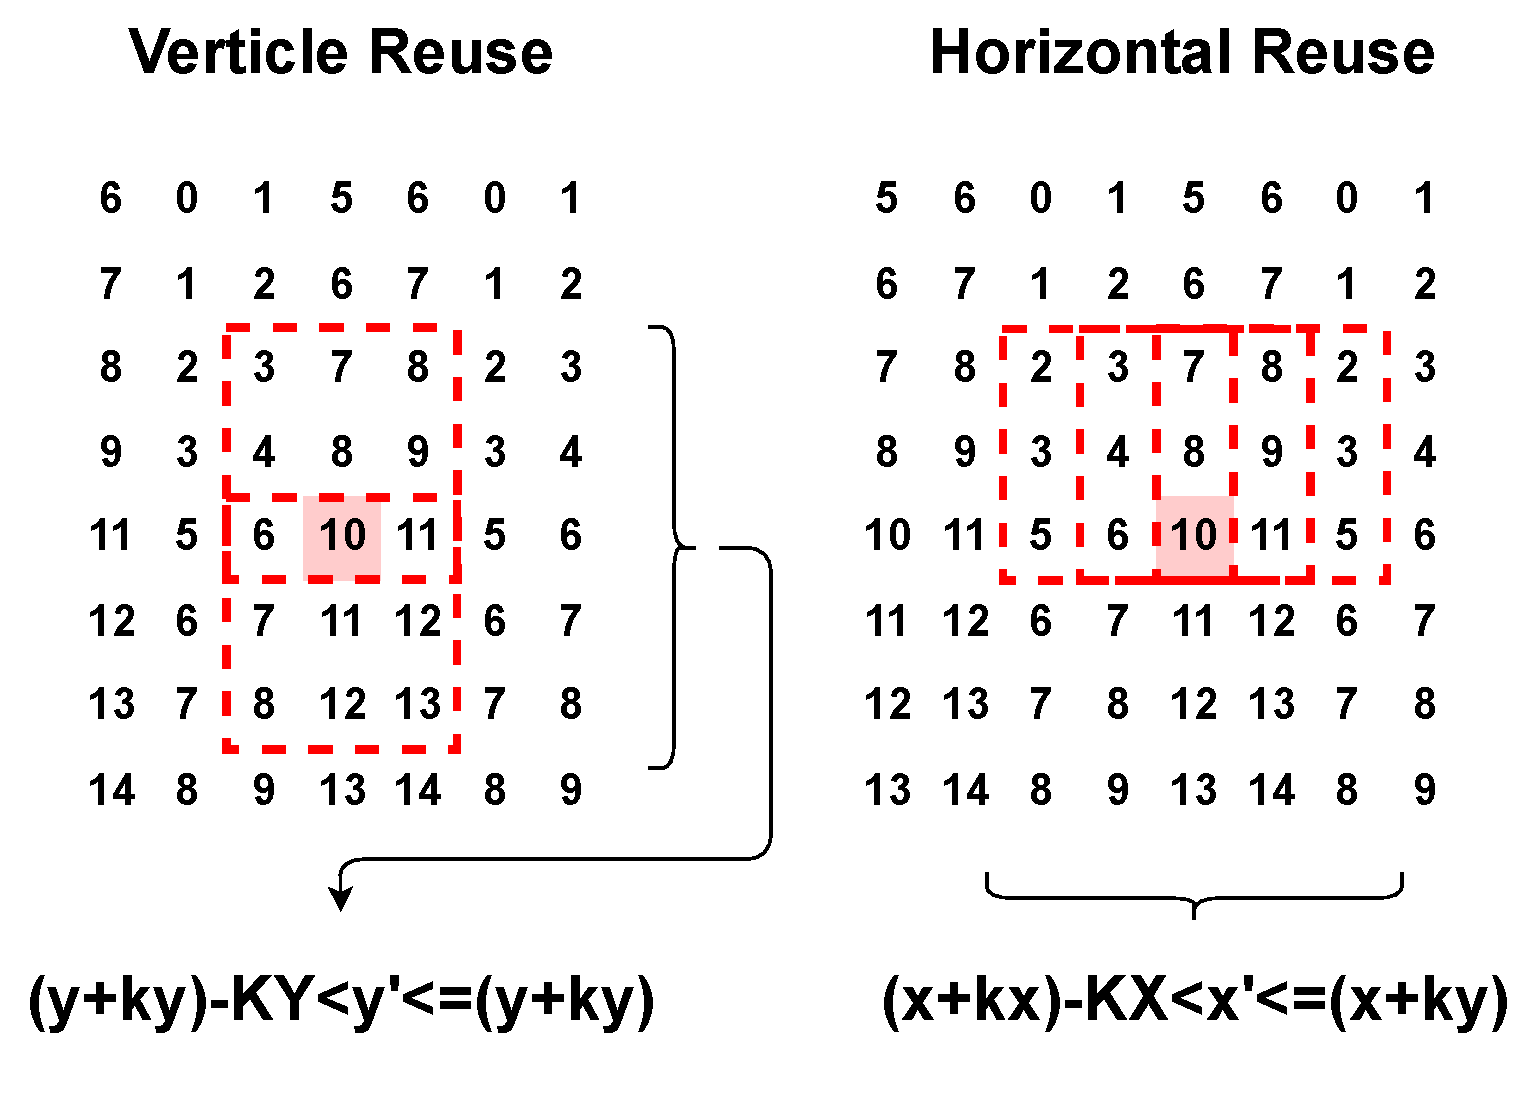
\includegraphics[scale=0.4]{fig/xy_reuse.pdf}
    \caption{IFmap Reuse Behavior w.r.t individual feature map channels}
    \label{fig:ifmap_xy_reuse}
\end{figure}

Within an individual IFmap channel, temporal reuse is exhibited w.r.t X and Y
loops. Given the complexity of the domain constraints of IFMAP\_XY\_REUSE in
\autoref{lst:poly:xy_reuse}, an illustration of the reuse behavior is available
in \figref{fig:ifmap_xy_reuse}. In \figref{fig:ifmap_xy_reuse}, individual
pixels within the kernel are reused based on the position of the sliding window
or stencil of the convolution in an IFmap channel. There are two primary
directions where that reuse is exhibited, vertical and horizontal with an IFmap
channel. The loops that control the verticle and horizontal stencil position in
the IFmap are the Y and X loops in the dataflow. Because kernel loops are fully
unrolled, the temporal reuse exhibited in \autoref{lst:poly:xy_reuse} occurs
accross unrolled kernel loop ports. To determine the appropriate memory
infrastructure to support that stencil based access pattern, we can apply the
technique in \cite{meeus} to construct a reuse chain that moves reused data
between urnolled kernel ports. The advantage of using a reuse chain is that the
temporal reuse that exists within an IFmap channel is relegated to a smaller
memory with lower memory access cost.

\cite{meeus} constructs a reuse chain for applications with a sliding window
access pattern that connects each unrolled kernel port with it's neighbors using
a FIFO or a shift register. If the temporal reuse distances between the accesses
of neighboring ports are constant \cite{meeus} uses a shift register, otherwise
they use a FIFO. The reuse distance between accesses of neighboring ports are
then converted into storage of the same size. So if two ports share the same
data but with a lag of 2 iterations in the iteration domain they're operating
in, then a shift register of size 2 can be placed between them. Similar to the
sliding window application explored in \cite{meeus} the reuse distances between
the unrolled kernel ports in the convolution dataflow are also constant. To
determine the reuse distances necessary between ports we can apply the analysis
in \autoref{lst:poly:xy_buffer_sizing:analysis} adapted from \cite{meeus} to
determine the sizing of the buffers in the reuse chain for IFmap accesses within
a channel. The analysis in \autoref{lst:poly:xy_buffer_sizing:analysis} assumes
a kernel size of 3x3. 


\begin{lstlisting}[caption=Determining buffer sizes in 3x3 convolutions, label={lst:poly:xy_buffer_sizing:analysis}]
    ID:=[IFMAP_Y, IFMAP_X] -> {S[y,x]:y>=0 and x>=0 and y<=IFMAP_Y-3 and x<=IFMAP_X-3};
    A0:=[IFMAP_Y, IFMAP_X] -> {S[y,x]->A[y+0,x+0]}*ID;
    A1:=[IFMAP_Y, IFMAP_X] -> {S[y,x]->A[y+0,x+1]}*ID;
    A2:=[IFMAP_Y, IFMAP_X] -> {S[y,x]->A[y+0,x+2]}*ID;
    A3:=[IFMAP_Y, IFMAP_X] -> {S[y,x]->A[y+1,x+0]}*ID;
    ...
    A8:=[IFMAP_Y, IFMAP_X] -> {S[y,x]->A[y+2,x+2]}*ID;

    R10:=(lexmin ((A1.A0^-1)*(ID<<ID)));
    R21:=(lexmin ((A2.A1^-1)*(ID<<ID)));
    R32:=(lexmin ((A3.A2^-1)*(ID<<ID)));
    ...
    R87:=(lexmin ((A8.A7^-1)*(ID<<ID)));
\end{lstlisting}

In \autoref{lst:poly:xy_buffer_sizing:analysis}, the iteration domain for the YX
loops are defined as functions of the IFmap dimensions passed as parameters (line 1).
The unrolled kernel loop IFmap accesses are then described using access maps
that map the iteration vector [y,x] to the associated IFmap access (lines 2-7).
Notice that the accesses are described as constant offsets added to access iterators y
and x. These constants represent the kernel loop iterators ky, and kx that are now
unrolled. For each neighboring pair of ports accessing the IFmap we can
determine the reuse behavior in (lines 9-10). Operations in lines (9-13) map
iterations where a port accesses a data element in IFmap with the earliest next
iteration in which the neighboring port accesses that same data element. The
distance between the accesses is then used as the reuse buffer size. The results
of the analysis are presented in \autoref{lst:poly:xy_buffer_sizing:results}.

\clearpage 

\begin{lstlisting}[caption=Polyhedral analysis of reuse in iscc for convolution loops, label={lst:poly:xy_buffer_sizing:results}]
R10;
$1 := [IFMAP_Y, IFMAP_X] -> { 
    S[y, x] -> S[y' = y, x' = 1 + x] : 
        0 <= y <= -3 + IFMAP_Y and 0 <= x <= -4 + IFMAP_X 
}
R21;
$2 := [IFMAP_Y, IFMAP_X] -> { 
    S[y, x] -> S[y' = y, x' = 1 + x] : 
        0 <= y <= -3 + IFMAP_Y and 0 <= x <= -4 + IFMAP_X 
}
R32;
$3 := [IFMAP_Y, IFMAP_X] -> { 
    S[y, x] -> S[y' = 1 + y, x' = -2 + x] : 
        0 <= y <= -4 + IFMAP_Y and 2 <= x <= -3 + IFMAP_X 
}
...
R87;
$8 := [IFMAP_Y, IFMAP_X] -> { 
    S[y, x] -> S[y' = y, x' = 1 + x] : 
        0 <= y <= -3 + IFMAP_Y and 0 <= x <= -4 + IFMAP_X 
}
\end{lstlisting}

In \ref{lst:poly:xy_buffer_sizing:results}, reuse distances between neighboring
ports depend on the relationship between the ports and whether their access offsets
are in the same row of the stencil or not. If two neighboring ports have unequal
ky offsets the reuse distance between them is IFMAP\_X-3. If two neighboring
ports have an equal ky offset the reuse distance is 1. An example of the first
case is lines 11-15 where the reuse distance between port 2 and port 3 is
IFmap-3. The evidence of that is that for any data accessed at port 3 with
iteration vector y, x that same data is accessed at port 2 at iteration vector
[y+1, x-2]. Based on the lexicographic ordering of iteration vector [y, x] and [y+1,
x-2], the distance between those two vectors is IFMAP\_X-3, or in terms of OFmap
dimensions X-1. Applying the same analysis to two ports in the same row (R10,
R21, R45, R87, ...) yields a reuse distance of 1 as evidence by the iteration
vectors of access [y, x] and [y, x+1] in all of the afformentioned neighboring
port pairs. 

Applying the results of the analysis in
\autoref{lst:poly:xy_buffer_sizing:results} with the previous template \autoref{fig:reuse_illus}
results in the updated template \autoref{fig:reuse_chain}.

\begin{figure}[]
    \centering
    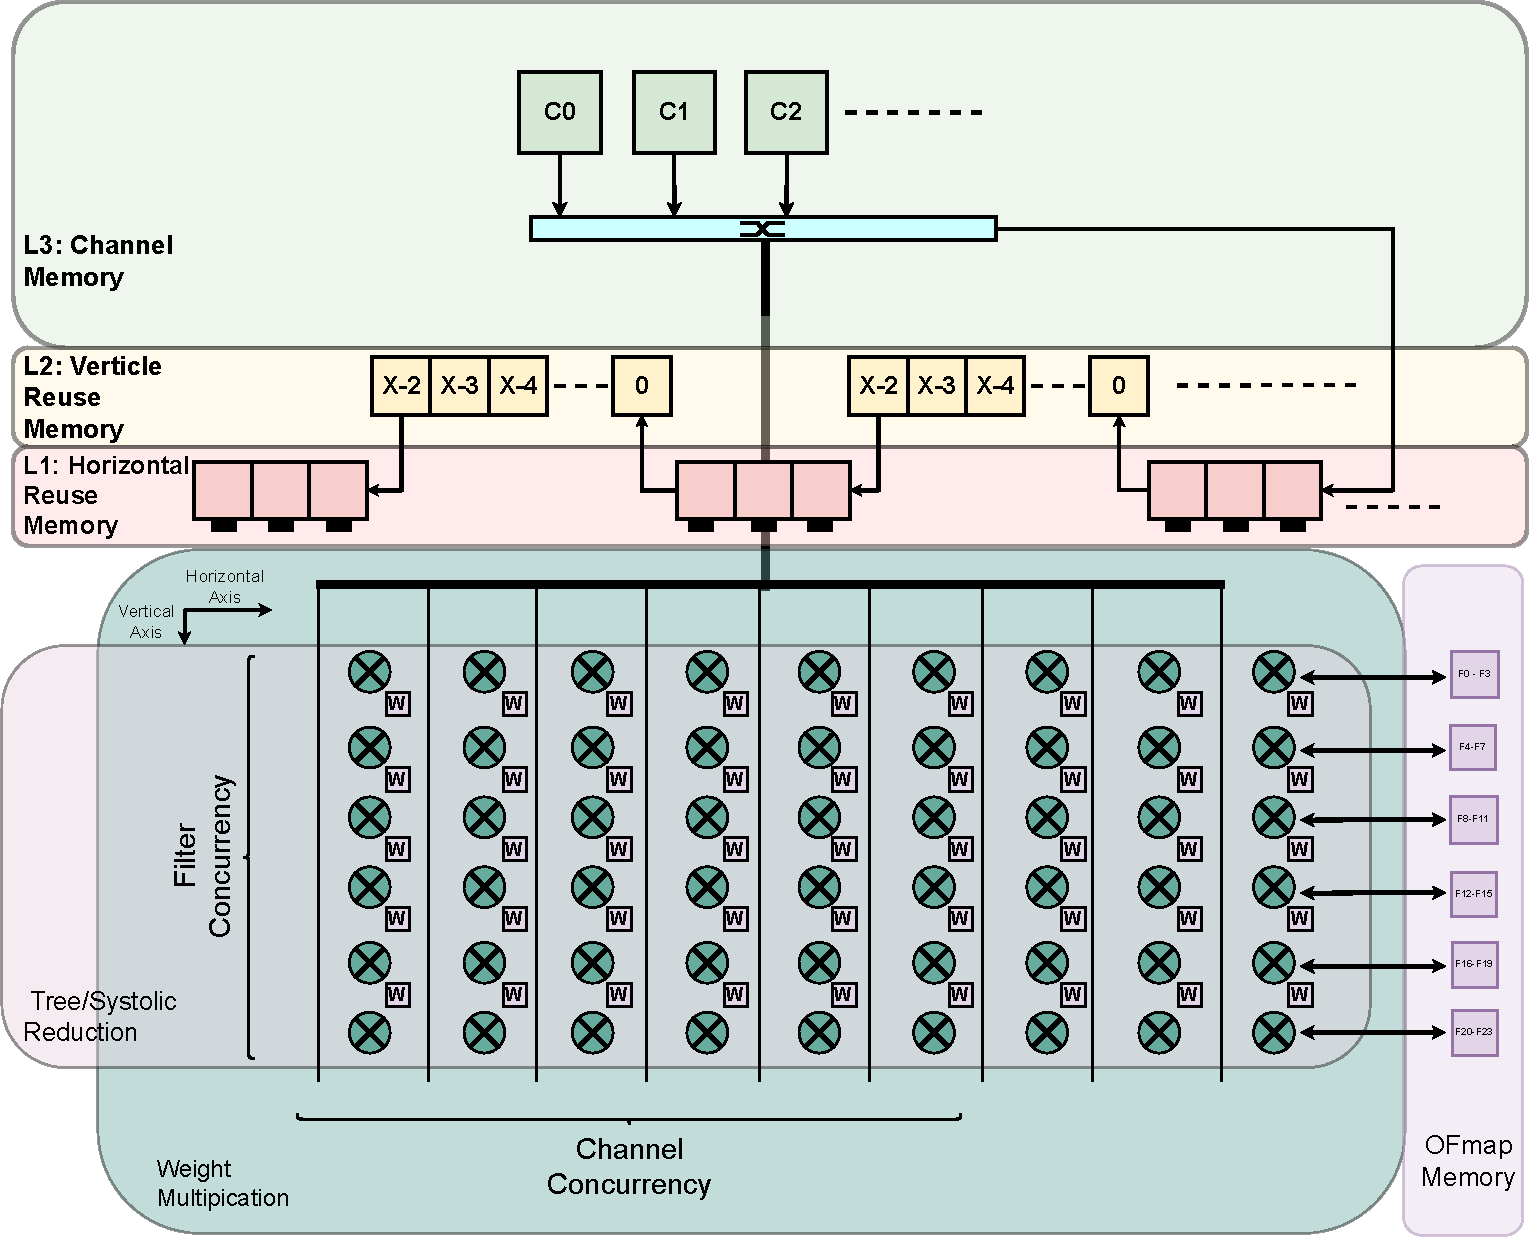
\includegraphics[scale=0.4]{fig/reuse_chain.pdf}
    \caption{Hardware template incorporating a reuse chain for reuse within an IFmap channel }
    \label{fig:reuse_chain}
\end{figure}


\subsection{Spatial Reuse Analysis}
\label{chap:hw_dse:spatial_reuse_analysis}

So now we know the hierarchy needed to express X and Y reuse in IFmap. Applying
the unroll factors in the target loops in the dataflow will yield a loop
structure similar to the one in \ref{lst:conv_loops_unrolled_fully}. Using the
convention established in \ref{chap:hw_dse:temporal_analysis}, each
\ac{MAC} statement in the unrolled loop body has an associated j index. In the
loop body there exists duplicate memory accesses across individual \ac{MAC}
spatial instances. Those duplicate accesses are highlighted in
\autoref{lst:conv_loops_unrolled_fully} and they are the origin of spatial reuse
in the dataflow. IFmaps exhibit spatial reuse with multicast communication w.r.t
to filter loops. OFmap exhibit spatial reuse with reduction communication
w.r.t to channel loops. Weights exhibit no spatial reuse 
 
\clearpage
\begin{lstlisting}[language=C, caption=Spatial reuse in fully unrolled kernel loops, label={lst:conv_loops_unrolled_fully}]
for(int f = 0; f < F; f+=F_T) // Filter loop
    for(int c = 0; c < C; c+=C_T) // Channel loop
        for (int y = 0; y < Y; y++) // FeatureMap Height
            for(int x = 0; x < X; x++) // FeatureMap Width
            {
                %\colorbox{green}{O[f+0][y][x]}% += W[f+0][c+0][0][0] * \ 
                                    %\colorbox{yellow}{I[c+0][y+0][x+0]}%; // j=0
                %\colorbox{green}{O[f+0][y][x]}% += W[f+0][c+0][0][1] * \
                                    %\colorbox{yellow}{I[c+0][y+0][x+1]}%; // j=1
                %\colorbox{green}{O[f+0][y][x]}% += W[f+0][c+0][0][2] * \
                                    I[c+0][y+0][x+2];  // j=2
                %\colorbox{green}{O[f+0][y][x]}% += W[f+0][c+0][1][0] * \ 
                                    I[c+0][y+1][x+2];  // j=3
                ...
                %\colorbox{red}{O[f+1][y][x]}% += W[f+1][c+0][0][0] * \
                                    %\colorbox{yellow}{I[c+0][y+0][x+0]}%; // j=C_T*KY_T*KX_T
                %\colorbox{red}{O[f+1][y][x]}% += W[f+1][c+1][0][1] * \
                                    %\colorbox{yellow}{I[c+0][y+0][x+1]}%; // j=C_T*KY_T*KX_T+1
                ...
                O[f+F_T-1][y][x] += W[f+F_T-1][c+C_T-1][KY_T-1][KX_T-1] * \ 
                                        I[c][y+KY_T-1][x+KX_T-1]; 
                                                    // j=F_T*C_T*KY_T*KX_T-1
                                        
            }
\end{lstlisting}

Applying the taxonomy in \autoref{fig:hw_taxonomy} to data elements that are
spatially reused, IFmap channels that are spatially reused across unrolled
filter loops can be broadcast with a bus. The reuse chain discussed in
\autoref{chap:hw_dse:temporal_analysis} can be thought of as a
Store\&Forward scheme to deliver individual IFmap channel data elements to the
\ac{PE}s for reduction into OFmaps.Weights reused for channel iteration and are
discarded. They exhibit no spatial reuse, just temporal. Therefore they should
be kept in small on chip buffers, preferably close to the computation they are
used in. OFmap exhibit spatial reuse across concurrent channels as well as
temporal reuse across channel sets as discussed in
\autoref{chap:hw_dse:temporal_analysis}. A reduction tree as in
\autoref{fig:reduction_styles}.a or a systolic array reduce and fwd as in
\autoref{fig:reduction_styles}.b are both possible assuming no restrictions
arising from synthesis. Combining the reuse chain derived in
\autoref{chap:hw_dse:temporal_analysis} with the required systolic
delays yields a simplification to the L1 memory present in
\autoref{fig:reuse_chain}. This simplification is discussed in
\autoref{chap:hw_dse:simplifying_hierarchy}.


\begin{figure}
    \centering
    \subfigure[]{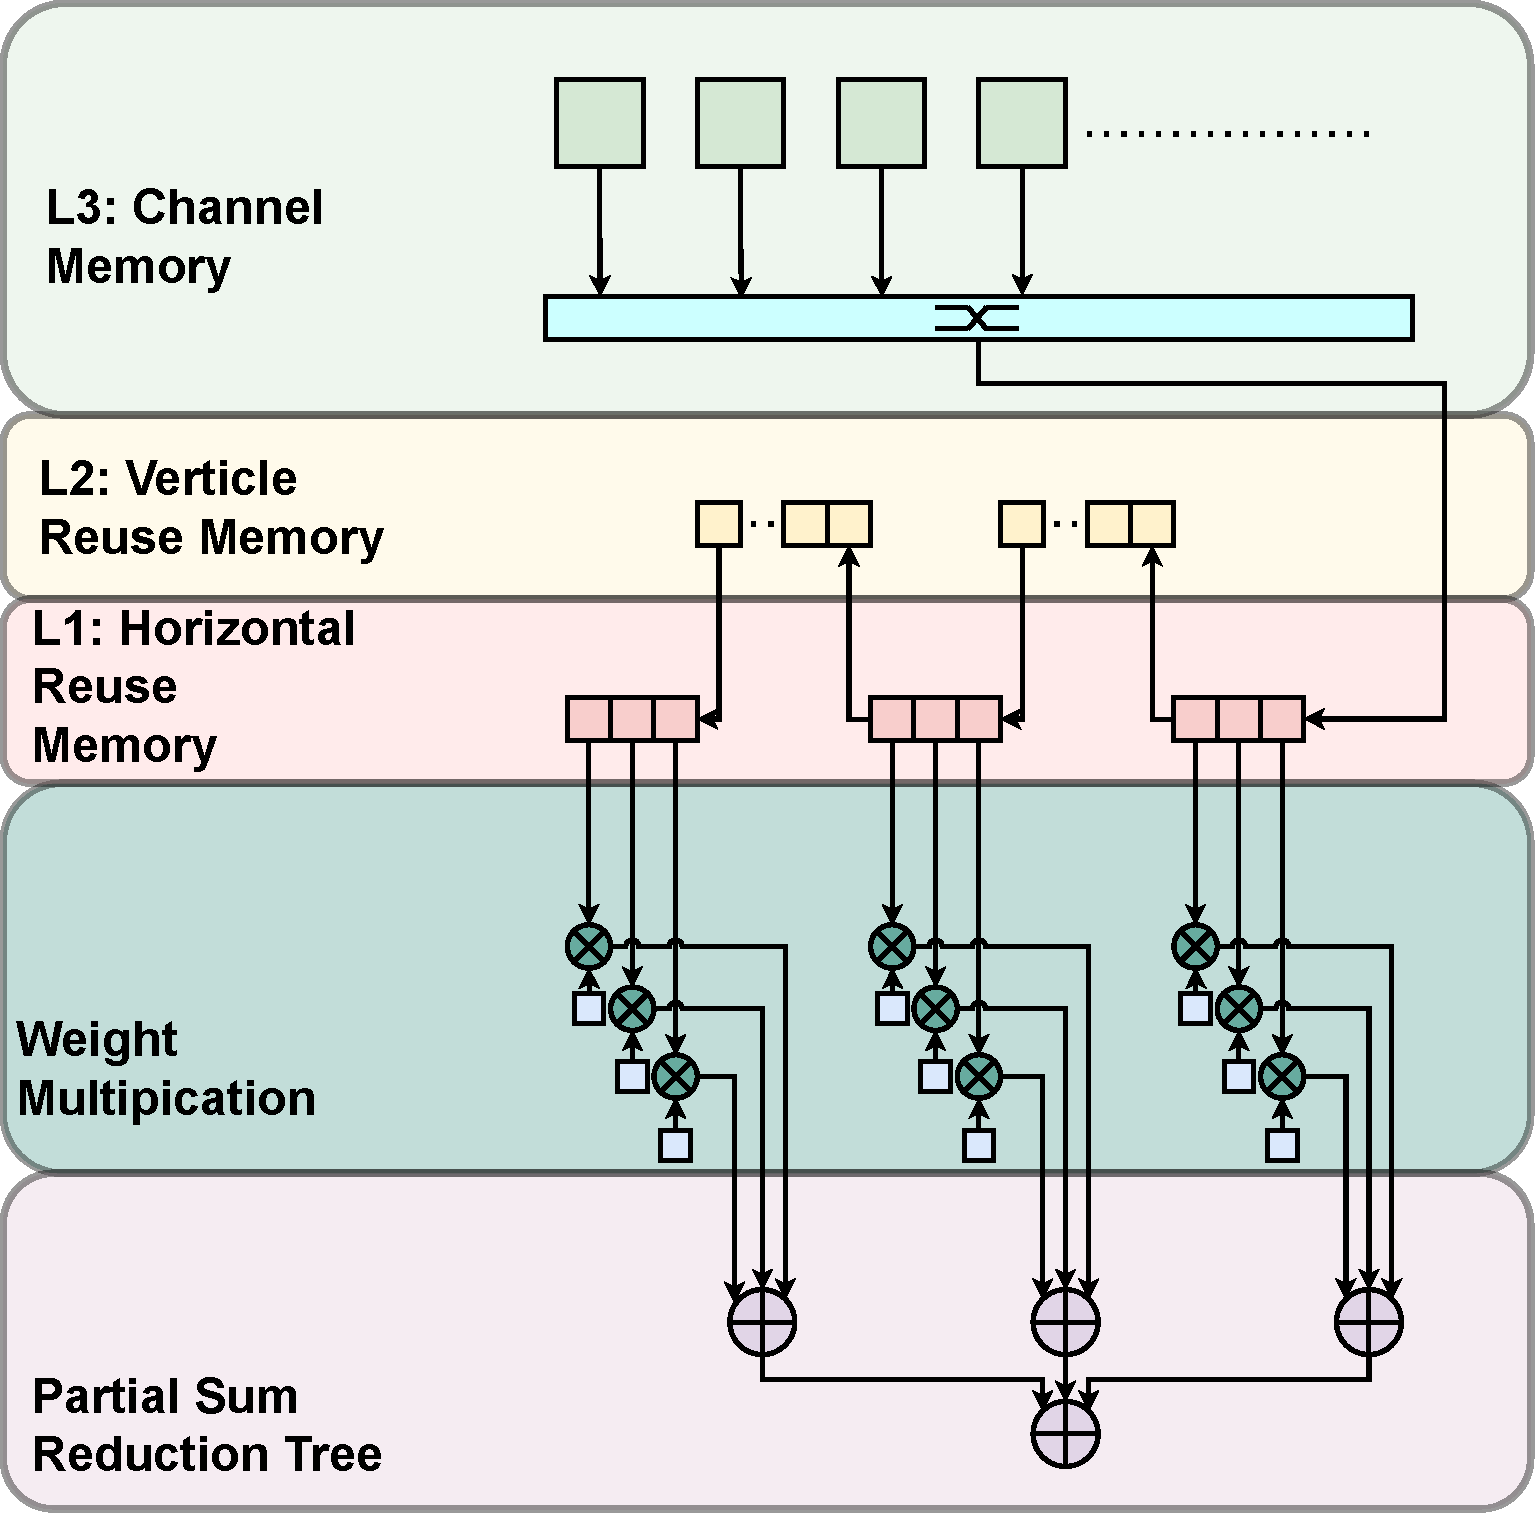
\includegraphics[width=0.5\textwidth]{fig/treeReduction.pdf}}
    \subfigure[]{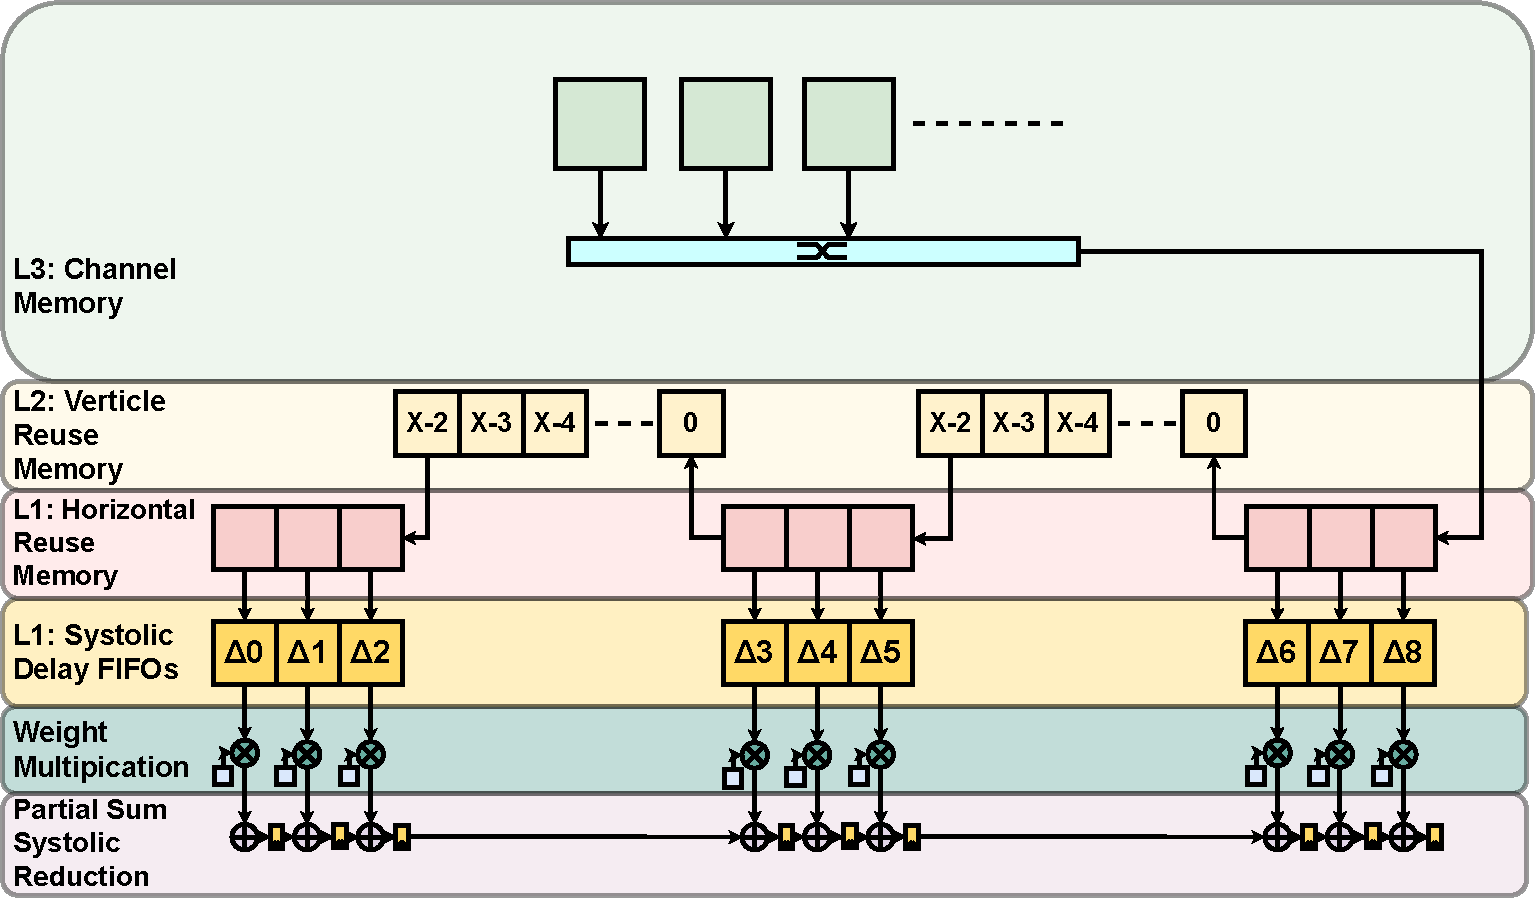
\includegraphics[width=0.7\textwidth]{fig/SystolicReduction.pdf}}
    \caption{Illustration of different partial sum reduction styles assuming kernel size is 3x3 (a) Tree Reduction (b) Systolic array reduction}
    \label{fig:reduction_styles}
\end{figure}

\subsection{Simplifying the memory hierarchy}
\label{chap:hw_dse:simplifying_hierarchy}

\begin{figure}[]
    \centering
    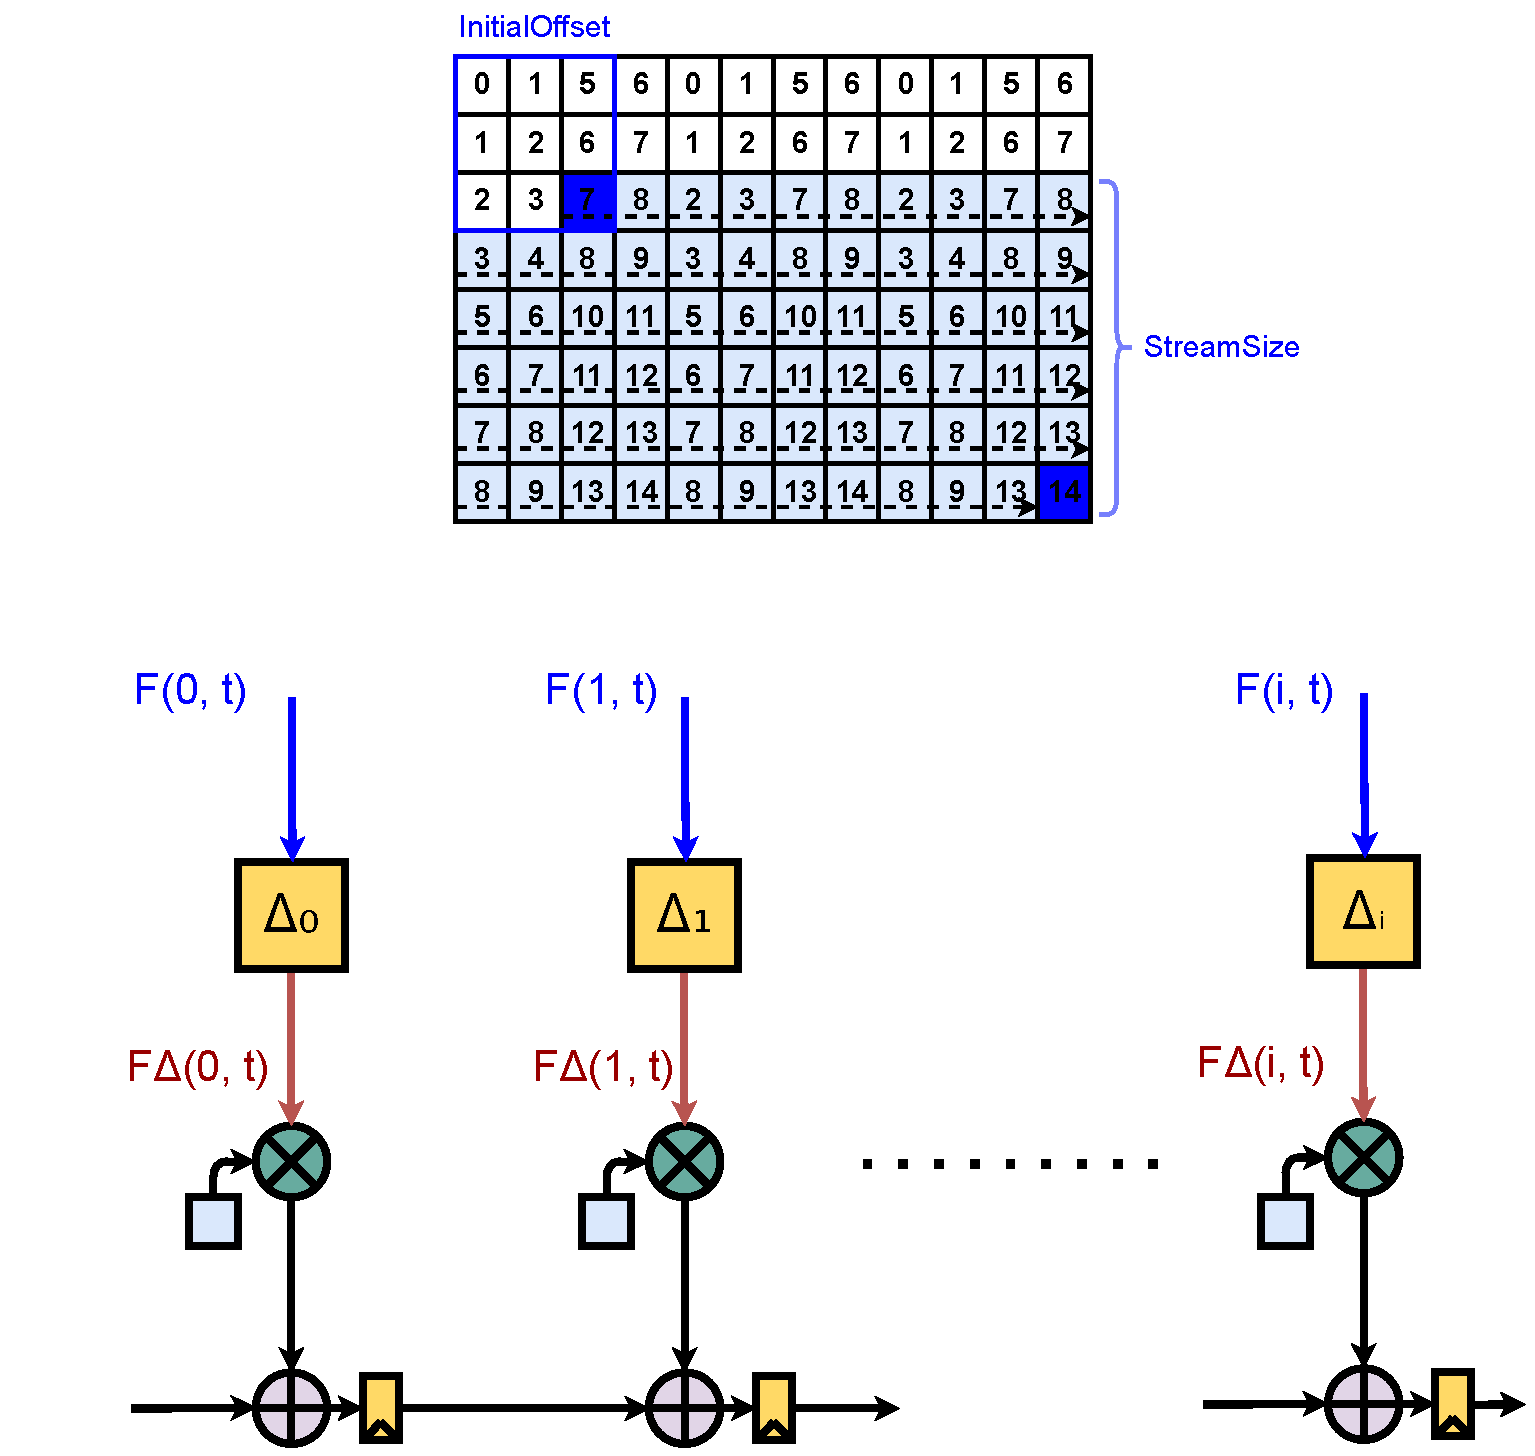
\includegraphics[scale=0.5]{fig/delayproof.pdf}
    \caption{Reinterpretation of IFmap memory hierarchy outputs as a stream function}
    \label{fig:delay_proof}
\end{figure}

We can reinterpret the accesses made by the IFmap memory hierarchy in
\autoref{fig:reuse_chain} as a stream function $F(i, t)$ whose output produces
element from an IFmap channel. The variable $i$ is the port index of IFmap
hierarchy and $t$ is the time in cycles since the beginning of the convolution
operation. A representation of this reinterpretation of the accesses made in the
IFmap memory hierarchy can be seen in \autoref{fig:delay_proof}. Since it's
always assumed that in direct mode kernel loops are unrolled fully the number of
ports into the IFmap memory hierarchy is always a multiple of $K^2$ where $K$ is
the size of the kernel being processed in direct mode. 

\begin{gather}
    IFmap \in R^{C\times n \times n} \xrightarrow{Reshape} IFmap \in R^{1\times Cn^2} \\
    Weight \in R^{F\times C\times K \times K} \\
    F(i, t)=    \begin{cases}
                    IFmap_{A(i, t)} & 0<=t < StreamSize \\
                    0 & else
                \end{cases} \\
    StreamSize = n(n-K)+(n-K) \\
    A(i, t) = InitialOffset(i) + t\\
\end{gather}

Each data element streamed from the IFmap depends on the an access function that
also takes the same variables $i$ and $t$. Depending on the port index $i$ the
access function for each port is composed on an initial offset in the IFmap and
the current cycle count. The number of cycles in which output from the IFmap
memory hierarchy can be produced is limited to the stream size of the IFmap
currently being processed. The stream size is a function of the IFmap dimensions
and the kernel Size. 

\begin{gather}
    InitialOffset = C_in^2+Y_in+X_i \\
    C_i = \lfloor \frac{\lfloor \frac{i}{K} \rfloor}{K} \rfloor \\
    Y_i = (\lfloor \frac{i}{K} \rfloor ) \bmod K\\
    X_i = i \bmod K = (i - \lfloor \frac{i}{K} \rfloor K)\\
\end{gather}

The initial offset function defines the initial index
offset in the IFmap the stream starts from for each port $i$. It can be
decomposed into three main offsets. A channel offset $C_i$, a row offset $Y_i$
and a column offset $X_i$. 

\begin{gather}
    F_\Delta(i, t) = \begin{cases}
    IFmap_{A_\Delta(i, t)} & \Delta_i<=t < \Delta_i+ StreamSize \\
    0 & else
    \end{cases} \\
    \Delta_i = i \\
    A_\Delta(i,t) = A(i, t) - \Delta_i\\
    % \hat{OFmap}(j) = \displaystyle\sum\limits_{i=0}^{ub(i)} A_\Delta(i, j+i)
\end{gather}

Under this new streaming based interpretation of the accesses in the IFmap
memory hierarchy, the delay elements in the systolic reduction scheme in
\autoref{fig:reduction_styles}.b are represented as time shifts in the stream
function $F(i,t)$. These time shifts are represented in the new delayed access
function $A_\Delta(i, t)$.

\begin{gather}
    A_\Delta(i,t) =  C_in^2+Y_in+(i - \lfloor \frac{i}{K} \rfloor K) + t- i\\
    A_\Delta(i,t) =  \lfloor \frac{\lfloor \frac{i}{K} \rfloor}{K} \rfloor^2+(\lfloor \frac{i}{K} \rfloor ) \bmod K + \underbrace{(- \lfloor \frac{i}{K} \rfloor K)}_{X'_i} + t\\
    % \hat{OFmap}(j) = \displaystyle\sum\limits_{i=0}^{ub(i)} A_\Delta(i, j+i)
\end{gather}

\begin{figure}[]
    \centering
    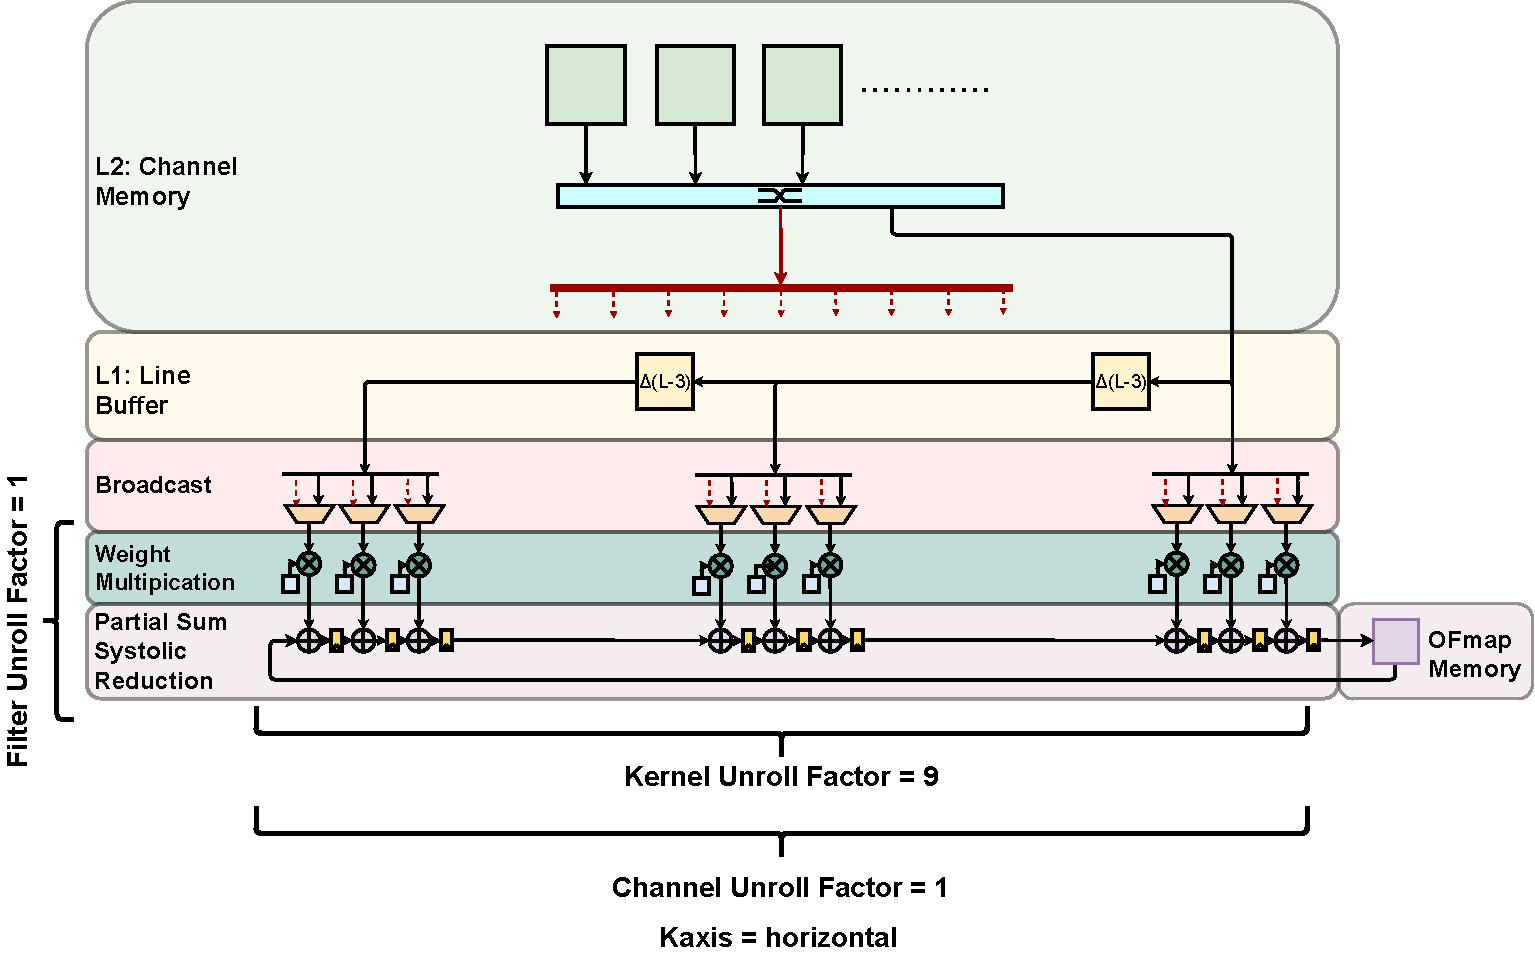
\includegraphics[scale=0.36]{fig/hybrid3x3Gemm.pdf}
    \caption{Using a systolic reduce and forward to calculate OFmaps}
    \label{fig:simplified_systolic_reduction}
\end{figure}

Substituting the InitialOffset function in $A_\Delta$  allows us to simplify the
column offset. This yields a new column offset $X'_i$. The final delayed access
function's initial offset becomes insensitive to changes in the port index $i$
that are not multiples of $K$. This allows us to remove the lowest layer memory
along with the systolic array delays in \autoref{fig:reuse_chain} and replace
both layers with just a series of broadcast buses that span consecutive $K$
groups of IFmap ports provided that we relax the start time constraints to the
$\lceil \frac{i}{K} \rceil$ for each group of ports $\lfloor \frac{i}{K}
\rfloor$. Delays in accessing IFmap data elements accross $K$ groups of ports
as well as accross $K^2$ groups of ports accessing different channels still
remain. This simplifying the hierarchy by removing the systolic delays thus still
requiring complex delayed reads from the IFmap hierarchy which necessitates smart
SRAMS whose access times can be programmed. A discussion of these smart memories
is presented in \autoref{chap:acc_sched:primitives:da-sram}. The final
hardware implementation with the added IFmap memory hierarchy optimization
discussed in this section is given in
\autoref{fig:simplified_systolic_reduction}.
\autoref{fig:simplified_systolic_reduction} shows the broadcast busses for every
group of 3 processing engines as well as the 1x1 vertical broadcast busses
highlighted in red. 

\section{HERO-T: A Hybrid GEMM and Direct Conv. Accelerator Template}
\label{chap:hero}

TEMPO's analytical model is hardware implementation agnostic
Tempo optimizes utilization given a library of networks + a pe budget
TEMPO reports average utilization, latency, and access count 
statistics
Then move on hero-t-sim to cycle accurate simulation results
Show performance for some popular networks

\begin{figure}[ht]
    \centering
    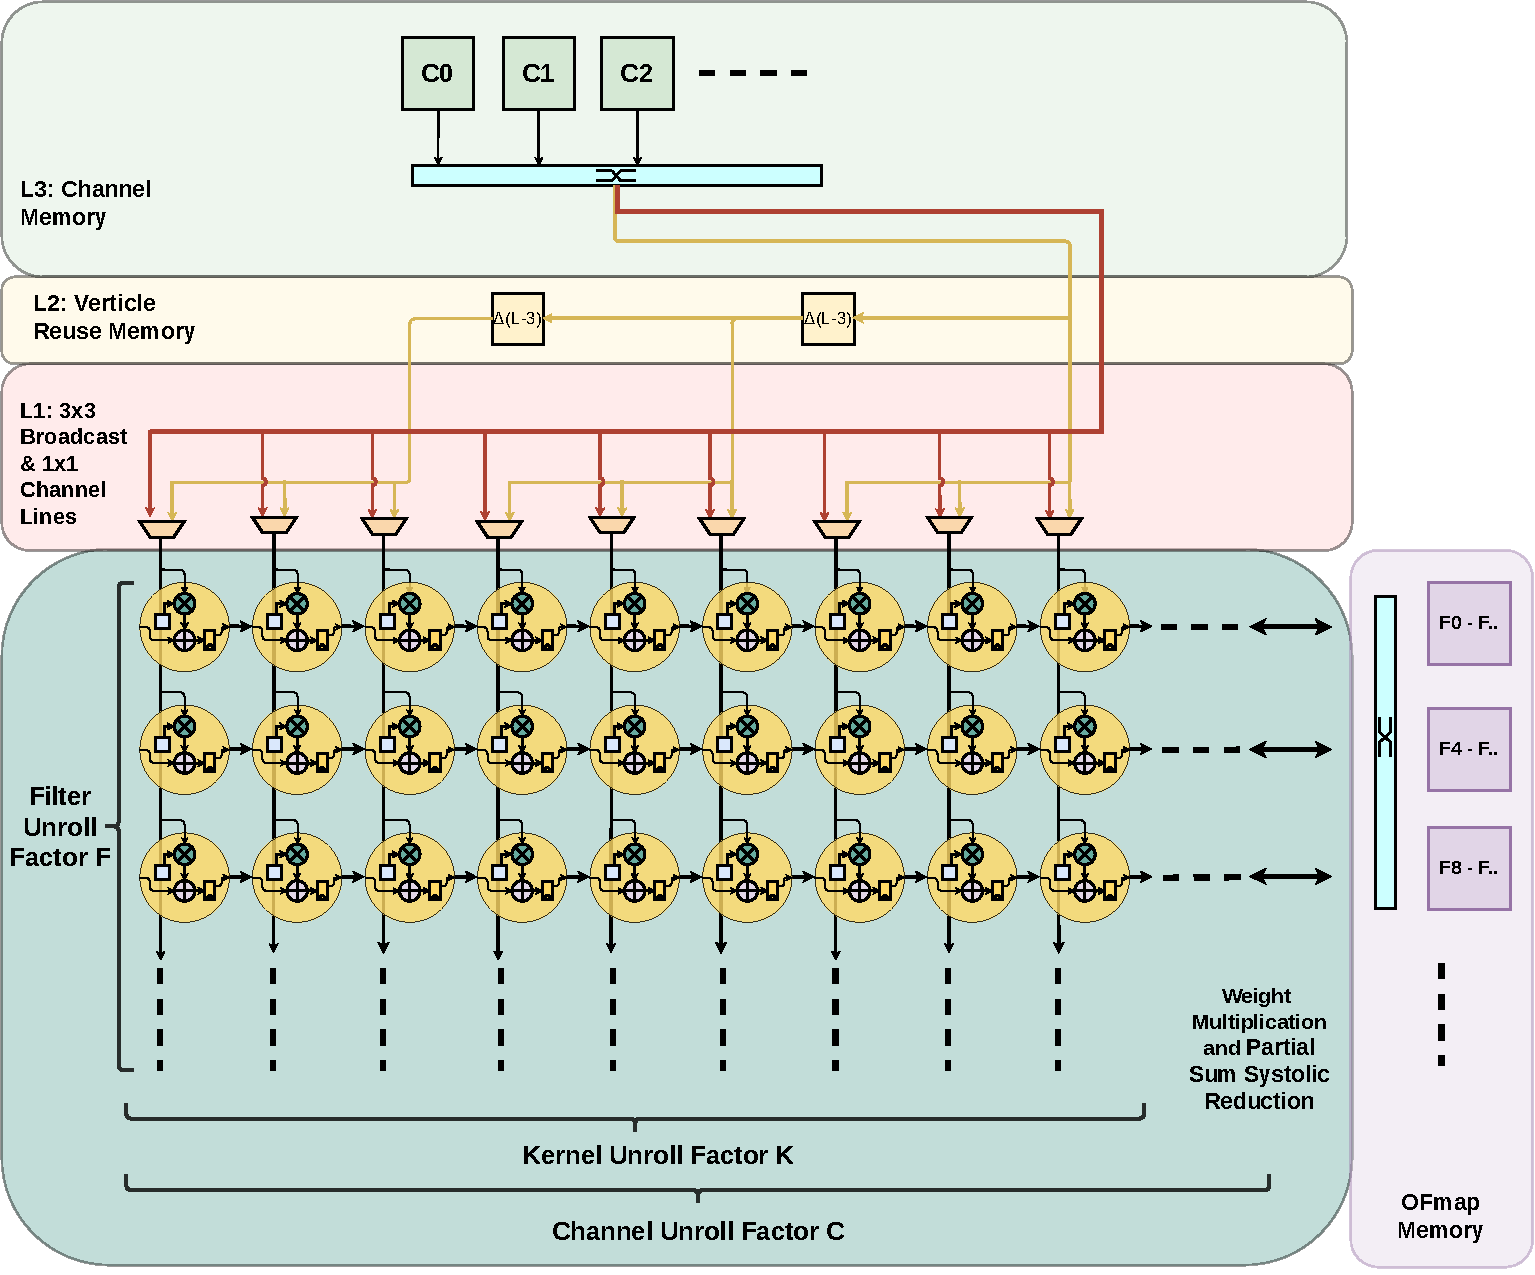
\includegraphics[scale=0.58]{fig/hero-t-horizontal.pdf}
    \caption{Hardware Implementation Taxonomy adapted from \cite{maestro}}
    \label{fig:hw_taxonomy}
\end{figure}

\begin{figure}[ht]
    \centering
    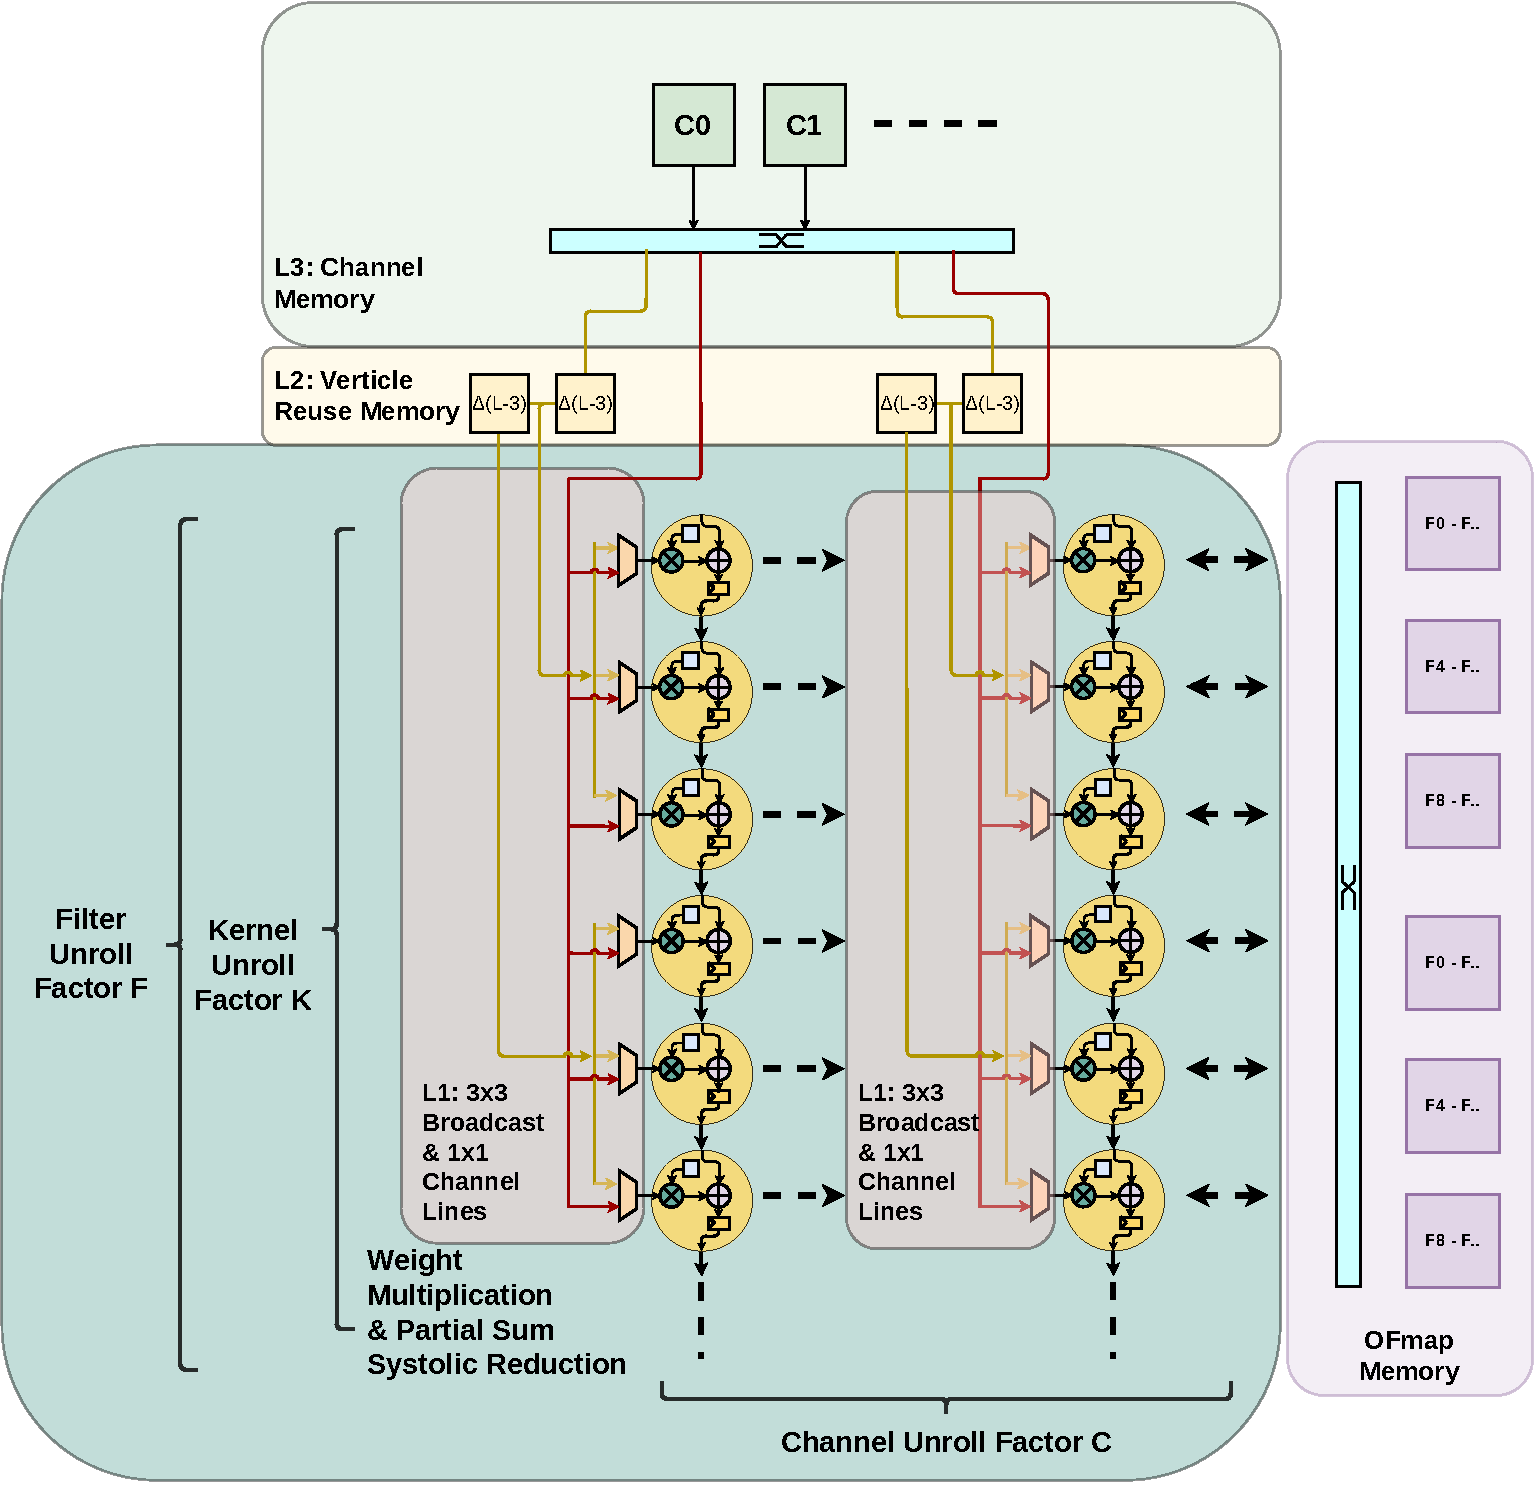
\includegraphics[scale=0.58]{fig/hero-t-verticle.pdf}
    \caption{Hardware Implementation Taxonomy adapted from \cite{maestro}}
    \label{fig:hw_taxonomy}
\end{figure}




\chapter{Architecture Dimensioning}
\label{chap:conv_gemm_equiv}

\section{Layer Equivalence}

Accelerator generality can be maintained by supporting general matrix
multiplication operations as well as convolution operations common in many
modern deep neural networks. Convolution operations can be converted into
general matrix multiplication through the use of lowering and lifting techniques
like Im2col discussed in \cite{cafe_con_troll}. To support matrix multiplication
within a convolution accelerator we can reporpose existing compute and memory
hardware on chip to perform both GEMM and convolutions operations or we can
establish a mathematical equivelence between GEMM operations and Conv by
reinterpret GEMM into a special case of convolution, namely convolutions with a
1x1 kernel size. This avoids the overhead of reporposing existing convolution
hardware to support GEMM. In \autoref{chap:conv_gemm_equiv:proof}, a proof for
the equivelence between GEMM and 1x1 Convolutions is given. Additionally, in
\autoref{chap:conv_gemm_equiv:application} the afformentioned proof will be used
in tandem with the approach in \cite{cafe_con_troll} to provide support for
arbitrary convolution operations. Finally in
\autoref{chap:conv_gemm_equiv:overhead} a discussion of the overheads associated
with the approach in \autoref{chap:conv_gemm_equiv:application} is given.

\clearpage

\subsection{Functional equivelence between GEMM and 1x1 Convolutions}
\label{chap:conv_gemm_equiv:proof}

We can establish functional equivelence between GEMM and 1x1 convolutions with
the following proof. An illustration of this proof is given in
\autoref{fig:gemmTo1x1Conv}.  
Given two matricies $A\in \mathbb{R}^{Z \times C}$ and $B \in \mathbb{R}^{C
\times F}$, let $R \in \mathbb{R}^{Z\times F} = A.B$. A different way to express
the matrix multiplication $A.B$ is \autoref{math:gemm_array_notation}.  

\begin{equation}
    \begin{aligned}
        R[z][f] = \displaystyle\sum\limits_{c=0}^{C-1}A[z][c]\times B[c][f] \\ \forall z\in[0, n^2-1]
    \end{aligned}
    \label{math:gemm_array_notation}
\end{equation}

Transposing $A$ and $B$ yields $\hat{A} \in \mathbb{R}^{C\times Z}$ and $\hat{B} \in
\mathbb{R}^{F\times C}$. Using the identity $(A.B)^T = B^T.A^T$ we can rewrite
\autoref{math:gemm_array_notation} as
\autoref{math:gemm_array_notation_transpose} where $\hat{R} \in
\mathbb{R}^{F\times Z}$

\begin{equation}
    \begin{aligned}
        \hat{R}[f][z] = \displaystyle\sum\limits_{c=0}^{C-1}\hat{B}[f][c]\times \hat{A}[c][z] \\ \forall z\in[0, Z-1]
    \end{aligned}
    \label{math:gemm_array_notation_transpose}
\end{equation}

We can reshape $\hat{A}$ and $\hat{B}$ using \autoref{math:a_b_reshape} into 3D
tensors by adding an additional dimention of size 1 for $\hat{A}$ and 2
additional dimentions of size 1 for $\hat{B}$.

\begin{equation}
    \begin{aligned}
        \hat{A} \xrightarrow[]{Reshape} &\hat{A}  \in \mathbb{R}^{C \times Z\times 1}   &\hat{B} & \xrightarrow[]{Reshape} \hat{B}  \in \mathbb{R}^{F \times C\times 1\times 1} \\
    \end{aligned}
    \label{math:a_b_reshape}
\end{equation}

Applying \autoref{math:a_b_reshape} to
\autoref{math:gemm_array_notation_transpose} yields
\autoref{math:gemm_as_conv_1} where $\hat{R} \in \mathbb{R}^{F \times Z\times 1}
$ remains the transposed output of $A.B$. 

\begin{equation}
    \begin{aligned}
        \hat{R}[f][z][0] = \displaystyle\sum\limits_{c=0}^{C-1}\hat{A}[c][z][0]*\hat{B}[f][c][0][0] \\ \forall z \in [0, Z-1] 
        \end{aligned}
    \label{math:gemm_as_conv_1}
\end{equation}

Adding kernel summations to \autoref{math:gemm_as_conv_1} yields
\autoref{math:gemm_as_conv_2} which is equivelent to a 1x1 convolution of stride
1. To recover $R$ from $\hat{R}$ we can reshape $\hat{R}$ by removing the
last dimention and then transpose it. 

\begin{equation}
    \begin{aligned}
        \hat{R}[f][z][0] = \displaystyle\sum\limits_{c=0}^{C-1}\displaystyle\sum\limits_{k_x=0}^{1} \displaystyle\sum\limits_{k_y=0}^{1}\hat{A}[c][y+ky][x+kx]*\hat{B}[f][c][k_y][k_x] \\ \forall y \in [0, Z-1] \land x = 0
    \end{aligned}
    \label{math:gemm_as_conv_2}
\end{equation}

\begin{figure}[]
    \centering
    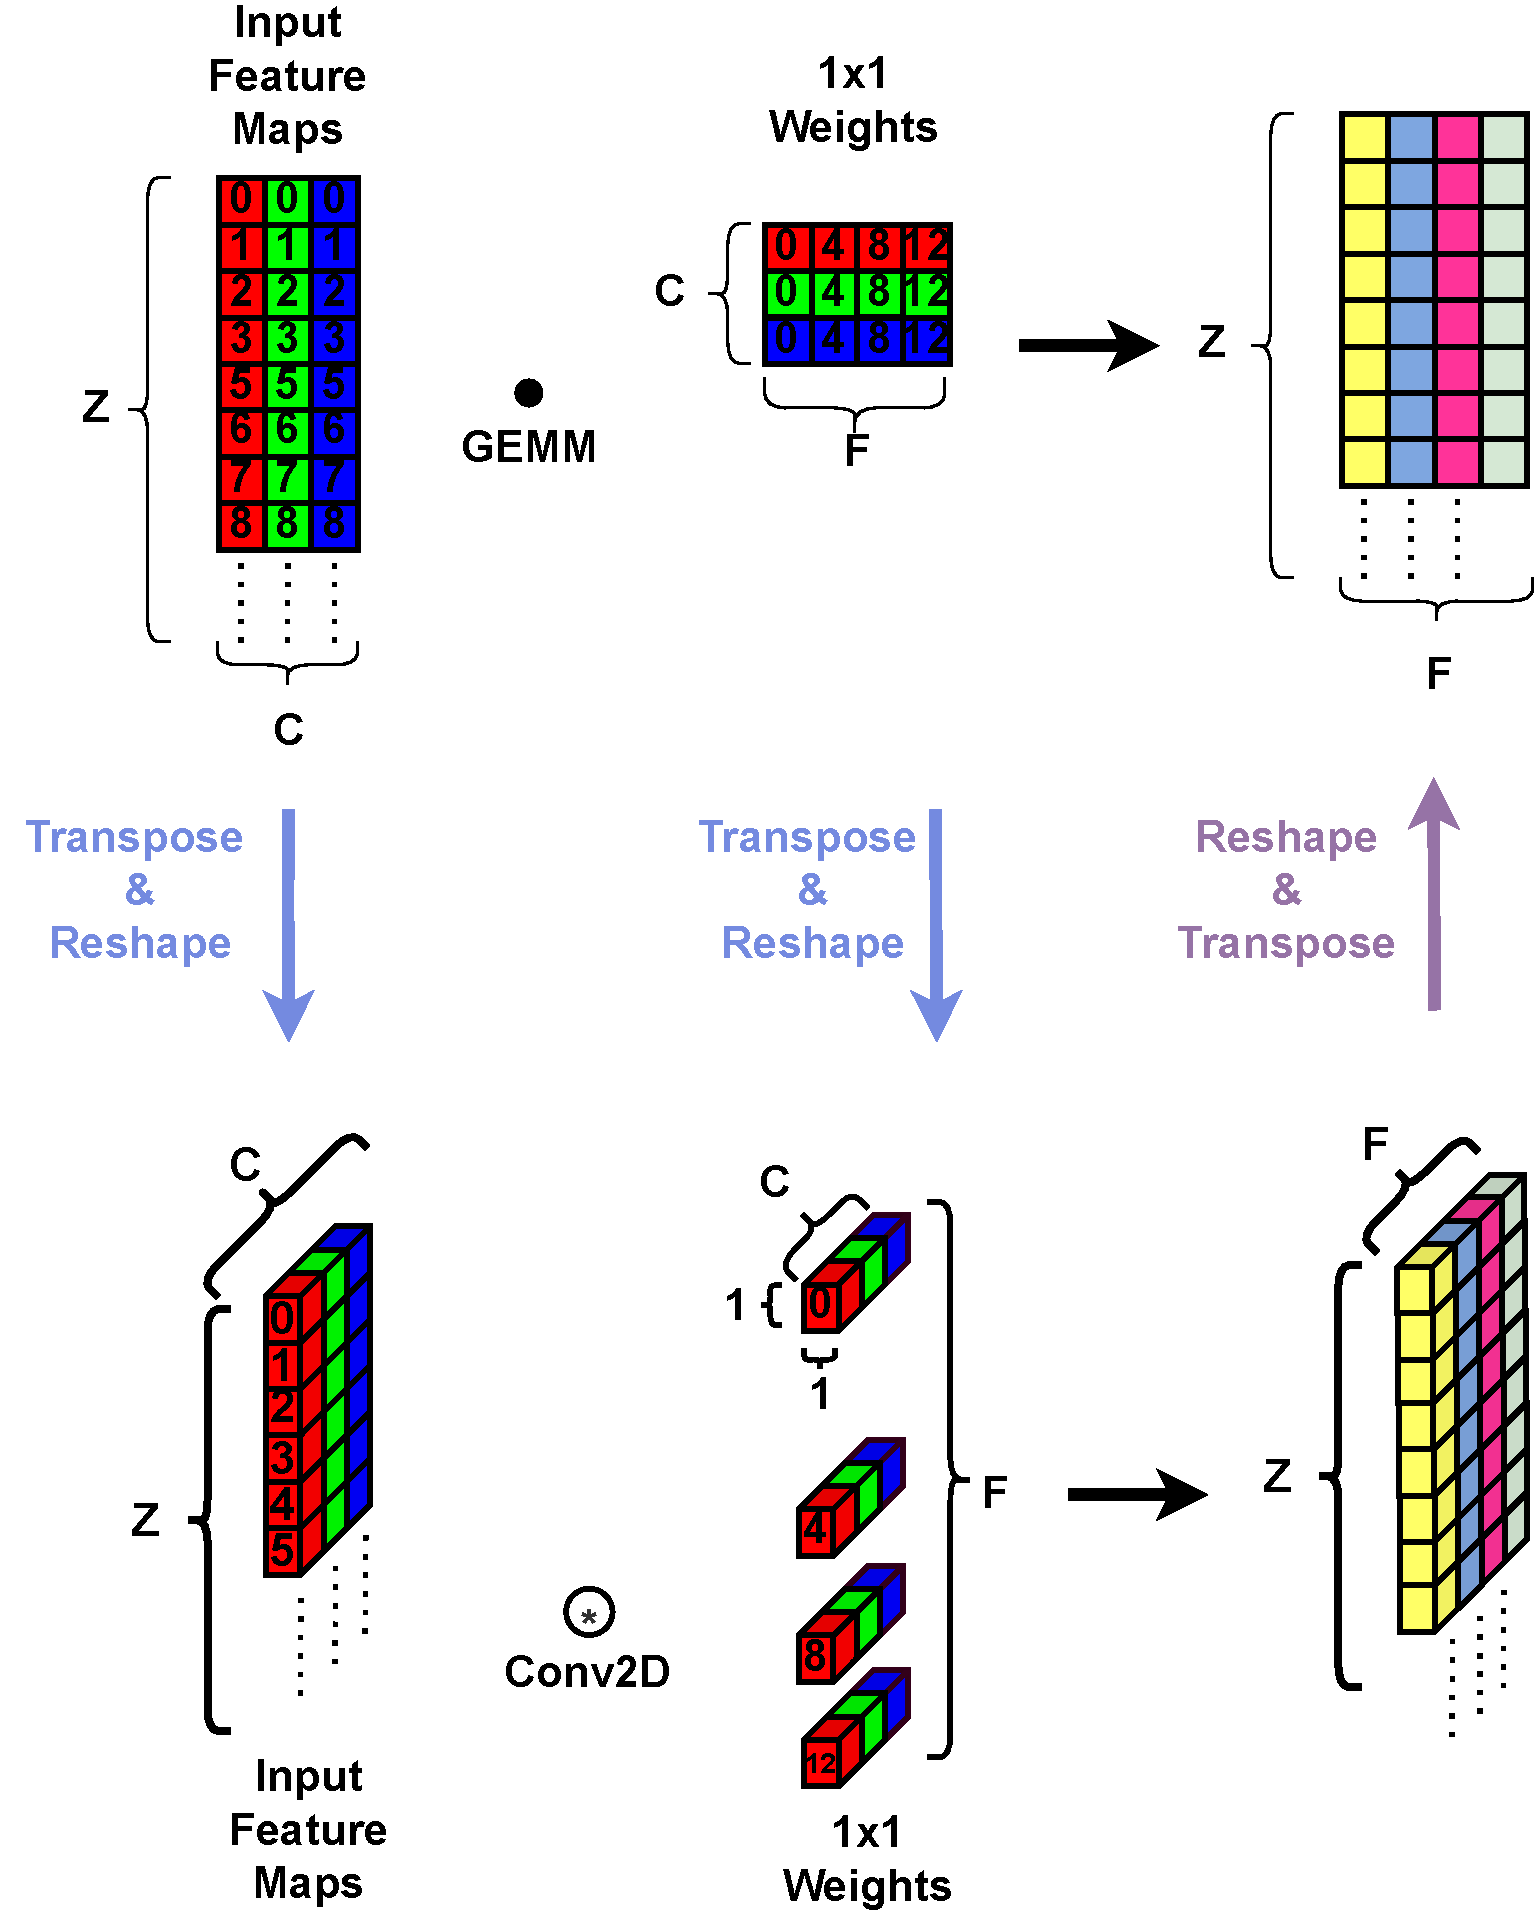
\includegraphics[scale=0.5]{fig/GemmTo1x1Conv.pdf}
    \caption{\ac{GEMM} and 1x1 Convolution Equivelence}
    \label{fig:gemmTo1x1Conv}
\end{figure}


\subsection{Supporting unsupported kernel sizes in a direct convolution accelerator}
\label{chap:conv_gemm_equiv:application}

We can support previously unsupported kernel sizes by combining the GEMM to 1x1
Conv conversion in \autoref{chap:conv_gemm_equiv:proof} with any tensor
lowering/lifting approach in \cite{cafe_con_troll}. Lowering converts a
convolution into a GEMM operation, and the approach in
\autoref{chap:conv_gemm_equiv:proof} reinterprets that operation as another 1x1
Convolution. This approach allows any convolution accelerator that can support
1x1 convolution operations to support any arbitrary convolution operation. A
visual illustration for this technique is presented in \autoref{fig:conv2gemm2conv}.
To demonstrate this approach we begin by lowering both IFmap using
\autoref{math:balanced_lowering_ifmap} and Weights using
\autoref{math:balanced_lowering_weight}. This results in two matricies IFmap and
Weights in \autoref{math:conv2gemm2conv:lowering}. Lowering should be performed
if the kernel size of the Weight tensor is unsupported $K' \notin
\{SupportedKernels\}$. 

\begin{equation}
    \begin{aligned}
        IFmap \in R^{C\times n\times n} & \xrightarrow[]{Balanced Lowering} \hat{IFmap} \in R^{nm\times K'C} \\
        Weight \in R^{F\times C\times K' \times K'} & \xrightarrow[]{Balanced Lowering} \hat{Weight} \in R^{K'C\times K'F} \\
    \end{aligned}
    \label{math:conv2gemm2conv:lowering}
\end{equation}

After lowering both tensors, we apply the transformations in
\autoref{math:conv2gemm2conv:transform} to reinterpret the anticipated GEMM
operation that occurs after lowering into a 1x1 convolution operation. The
transformations are composed of a transpose operation followed by a reshape
operation that appends additional dimentions of size 1 to both IFmap and
Weights. The transformations yields two new tensors $\hat{IFmap}$ and
$\hat{Weight}$.

\begin{equation}
    \begin{aligned}
        \hat{IFmap}^T \in R^{K'C \times nm} & \xrightarrow[]{Reshape} \hat{IFmap} \in R^{K'C \times nm \times 1} \\
        \hat{Weight}^T \in R^{K'F\times K'C} & \xrightarrow[]{Reshape} Weight \in R^{K'F\times K'C \times 1 \times 1} \\
        \end{aligned}
    \label{math:conv2gemm2conv:transform}
\end{equation}

After performing the transformations in \autoref{math:conv2gemm2conv:transform}
the output $\hat{OFmap_{prelift}}$ can be calculated after performing a 1x1
convolution in \autoref{math:conv2gemm2conv:conv} using the $\hat{IFmap}$ and
$\hat{Weight}$ tensors. 

\begin{equation}
    \begin{aligned}
        \hat{OFmap_{prelift}} \in R^{K'F\times nm \times 1} = \hat{IFmap}*\hat{Weight}
        \end{aligned}
    \label{math:conv2gemm2conv:conv}
\end{equation}

Finally we can lift $\hat{OFmap_{prelift}}$ by first reshaping it into a 2D
matrix by dropping the last dimension and then transposing it. After that, we
can apply balanced lifting in \autoref{math:balanced_lifting_ofmap} to get the
final OFmap in \autoref{math:conv2gemm2conv:lift}.

\begin{equation}
    \begin{aligned}
        \hat{OFmap_{prelift}} \in R^{K'F \times nm \times 1} \xrightarrow[]{Reshape} OFmap_{prelift} \in R^{K'F\times nm} \\
        OFmap_{prelift}^T \in R^{nm\times FK} \xrightarrow[]{Balanced Lifting} OFmap \in R^{F \times m \times m} \\
            \end{aligned}
    \label{math:conv2gemm2conv:lift}
\end{equation}

\begin{figure}[]
    \centering
    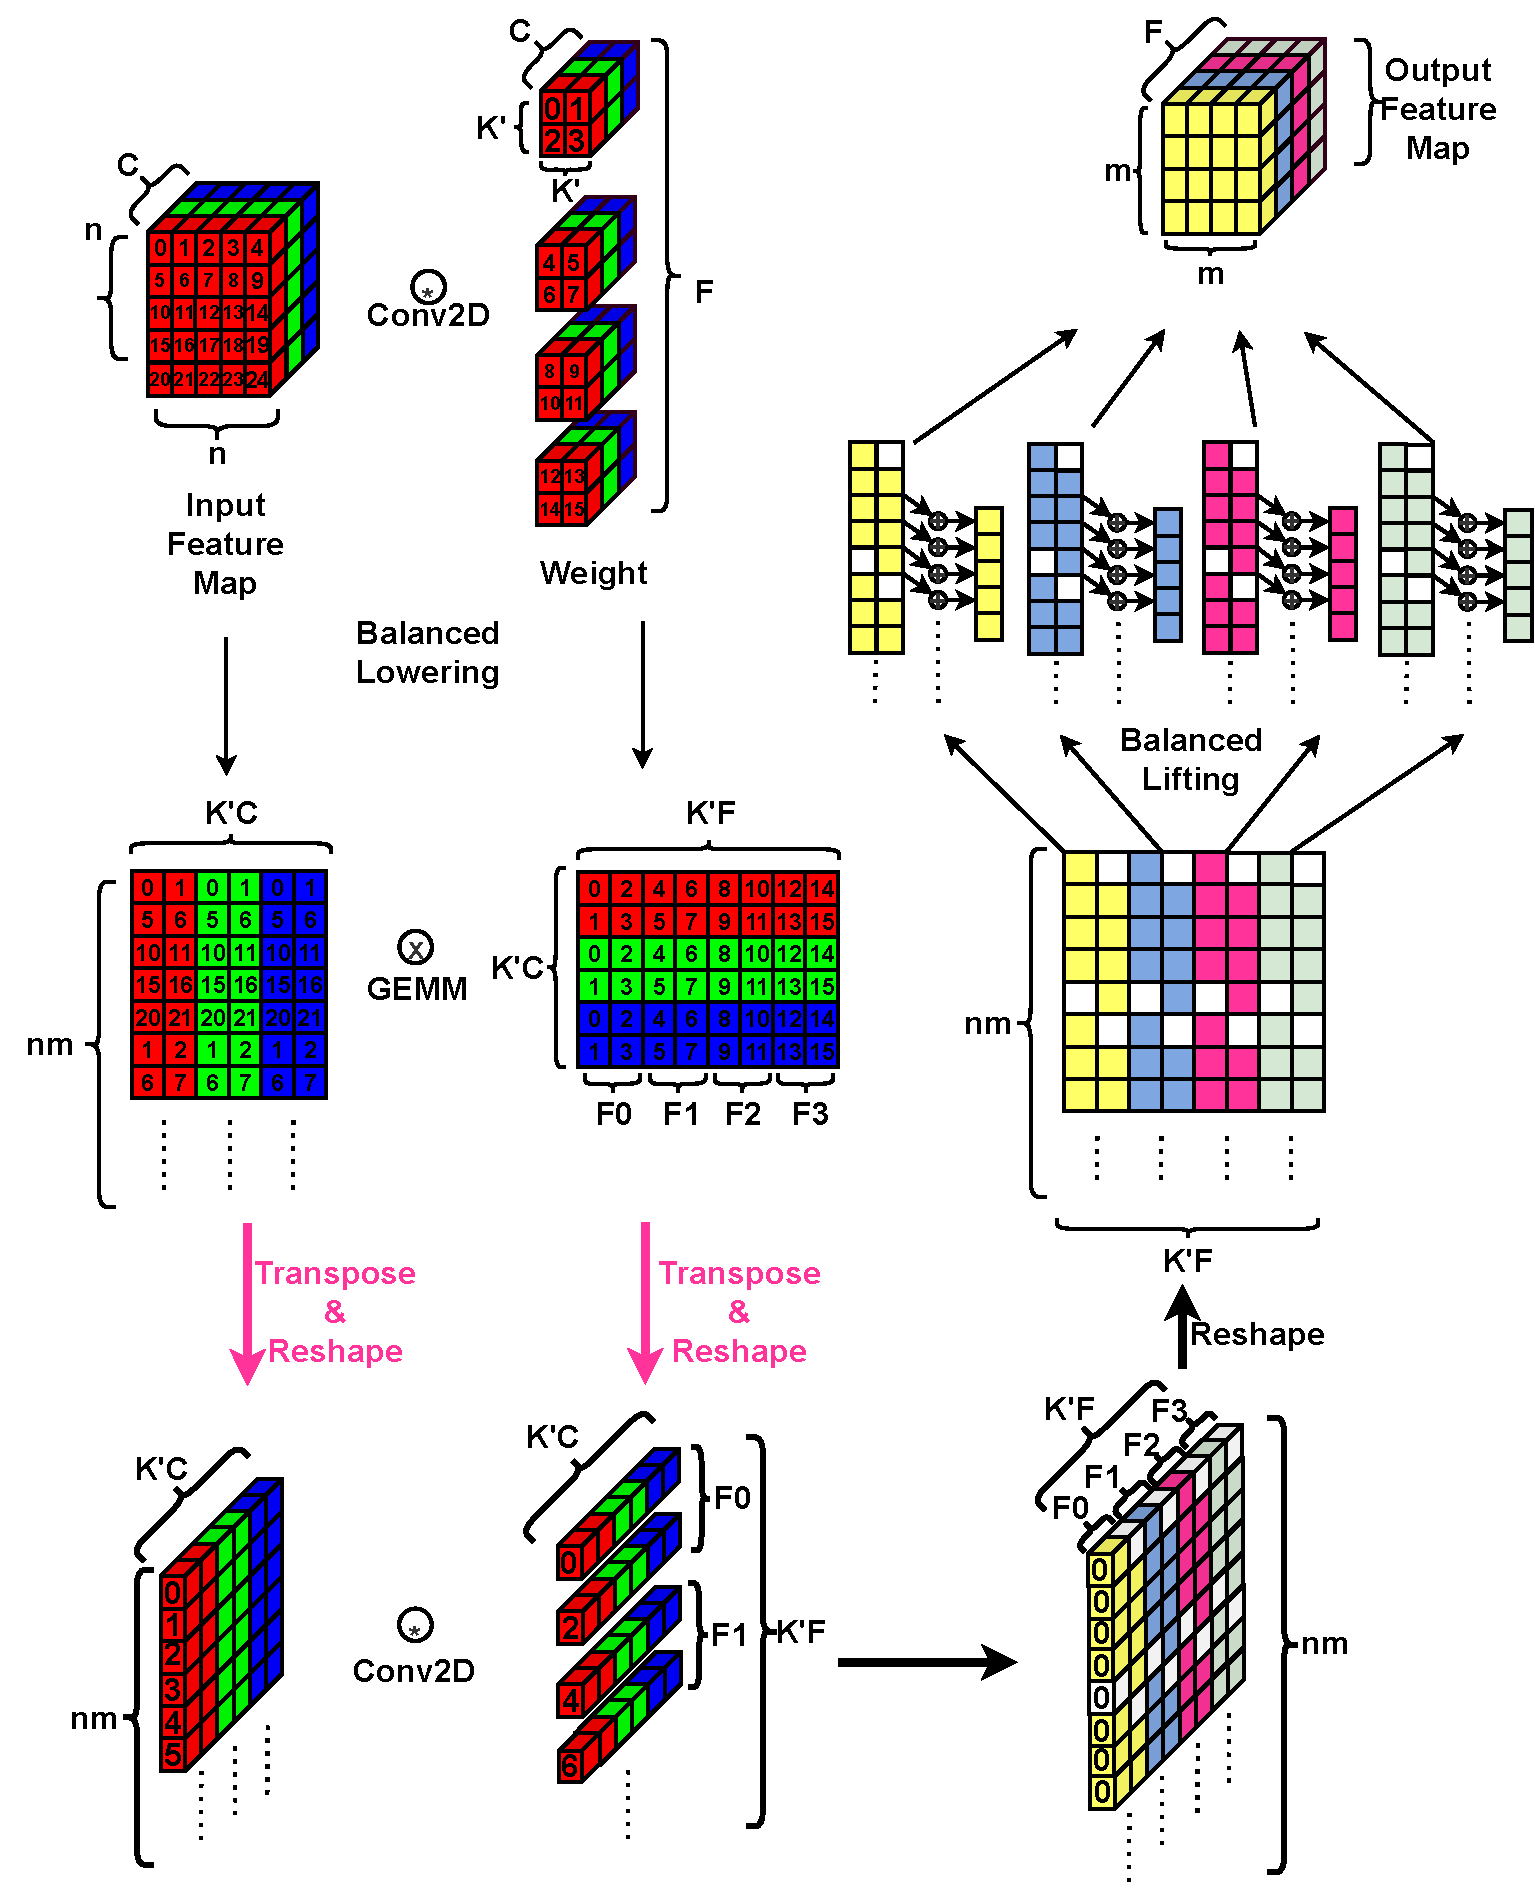
\includegraphics[scale=0.5]{fig/ConvToGemmToConv.pdf}
    \caption{Illustration of approach Conv2Gemm2Conv approach}
    \label{fig:conv2gemm2conv}
\end{figure}

\subsection{Overhead of extending support}
\label{chap:conv_gemm_equiv:overhead}

Lowering and lifting introduce additional overheads with regards to latency and
tensor sizing. The latency for performing balanced lowering and lifting is
$m^{2}K$ for a layer with a Weight tensor $\mathbb{R}^{F\times C\times K\times
K}$ and an OFmap tensor $\mathbb{R}^{F\times m\times m\times}$. While lowering
and lifting can be performed by a convolutions accelerator, in this thesis it is
assumed that a software processor on the same chip performs these operations.
Lowering also introduces duplicate data elements in the IFmap tensor thus
increasing it's overall size. In this thesis, it is assumed that on-chip memory
can account for this increase and that any additional DRAM accesses incurred
from lowering will be included in energy calculations when reporting energy
consumption of the accelerator.

To enable GEMM operations using the approach in
\autoref{chap:conv_gemm_equiv:proof} both input and output matricies are
transposed and reshaped. All reshape operations discussed in this chapter add a
dimention of size 1 to the data and they incur no data reorganization overhead.
Additionally, all transpose operations are assumed to be performed during
transfer to and from accelerator on-chip and thus incur no latency penalty. A
discussion of how transfers to and from on-chip memory can mask the latency of
transposing matricies is left as part of future work along with incorporating
lowering and lifting into the accelerator. 

% TODO: Mention savings as percentage of im2col
% https://www.desmos.com/calculator/p1qhtddjpa


\section{Exploring the dataflow design space with TEMPO}
\label{chap:dataflow_dse:exploring}

\begin{figure}[]
    \centering
    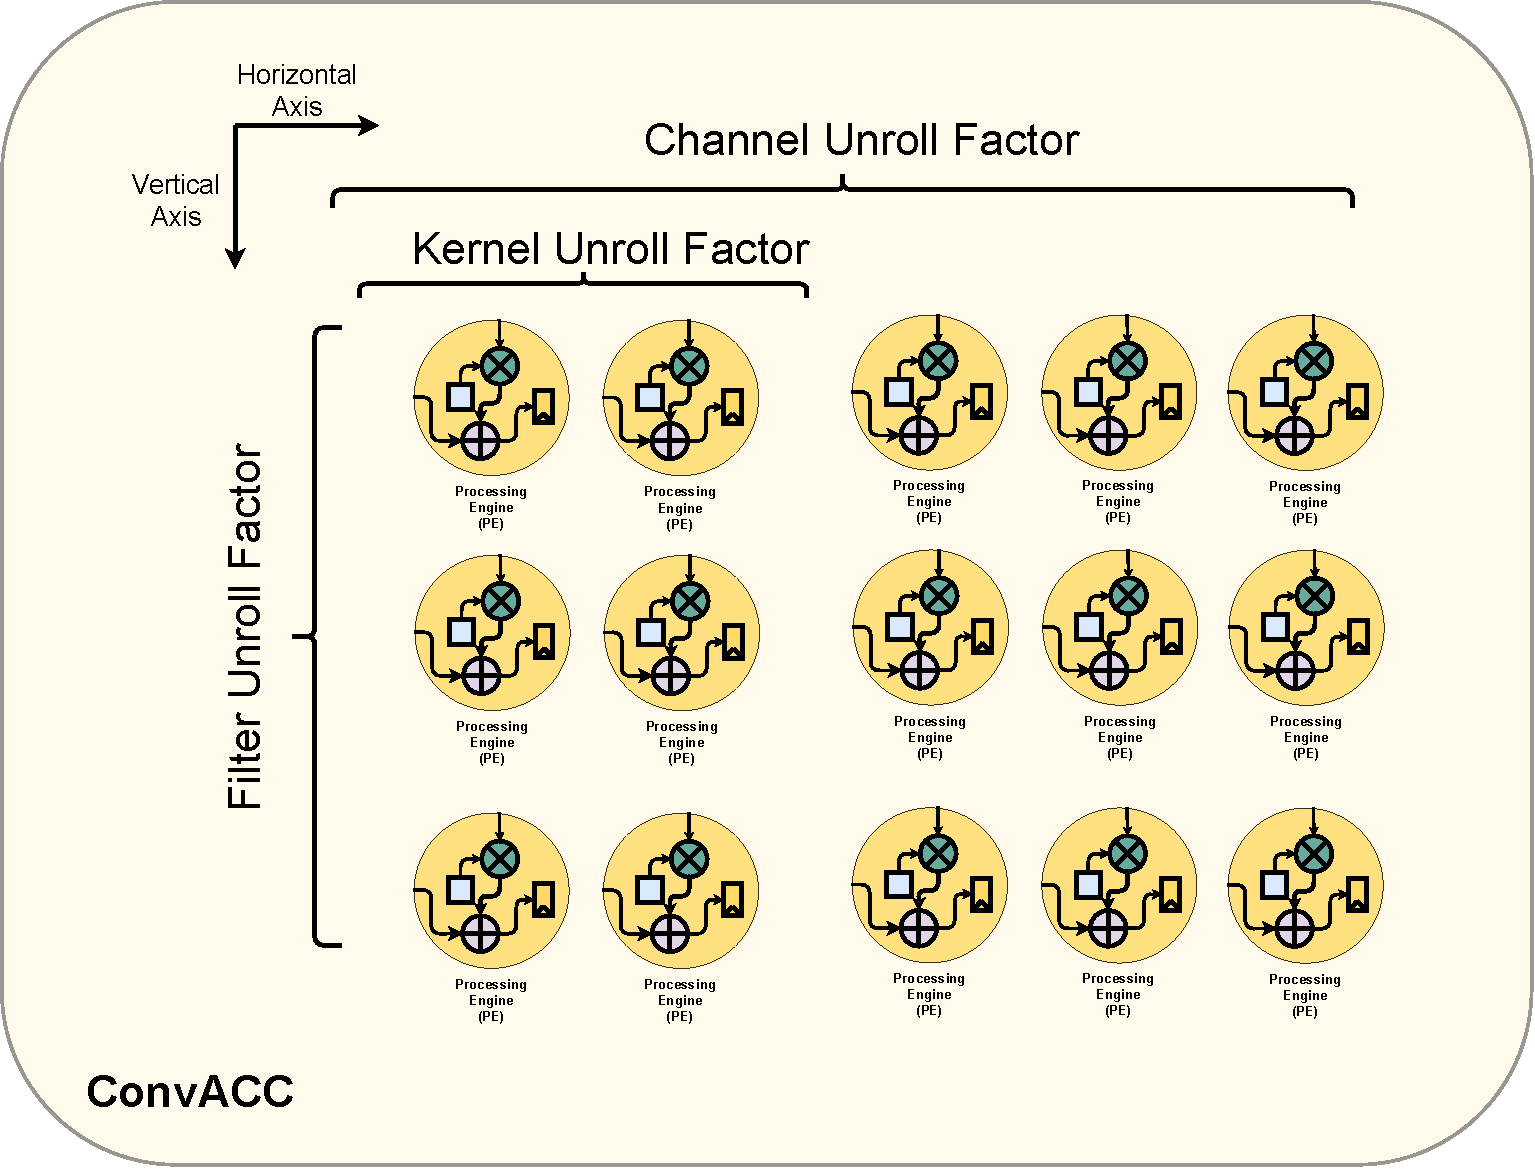
\includegraphics[scale=0.4]{fig/axis_mapping.pdf}
    \caption{\ac{GEMM} and 1x1 Convolution Equivelence}
    \label{fig:axis_mapping}
\end{figure}

From the previous section we have concluded that loops F, C, KY and KX are all
unroll targets, and KY and KX loops should be unrolled assuming that 1x1 and 3x3
kernels are supported directly. Additionally, the loop ordering of F and C loops
was discussed as well as it's implications with regards to on-chip memory
sizing. What remains of the dataflow design space is the unroll factors for F
and C loops as well as the accelerator spatial axis mapping for all unrolled
loops F, C, KY, KX. From this point these parameters will be referred to as
accelerator template paremeters from which a concrete accelerator instance can
be defined. These accelerator template parameters define the number of
processing engines allocated to process channels, filters, and kernels
concurrently in the concrete architectures. An illustration of this \ac{PE}
allocation is present in \autoref{fig:axis_mapping}. The space of possible
unroll factors is as large as the space of possible loop upperbounds for the
afformentioned unrolled loops. However, as discussed earlier, some combinations
of loop upperbounds are unlikely in real networks. Additionally, spatial axis
mapping affects the effective unroll factors when executing different
convolution layers than the ones assumed when unrolling said loops. This further
expands the design space of a concrete accelerator's template parameters. To
effectively explore the space of loop unroll factors and accelerator spatial
axis mapping we introduce \ac{TEMPO}, a dataflow exploration and analysis tool
used to optimize an accelerator's weight stationary dataflow based on a target
CNN library as well as an arbitrary objective function. A discussion of
\ac{TEMPO}'s algorithm model is presented in
\autoref{chap:dataflow_dse:exploring:algorithm} as well as it's analytical model
in in \autoref{chap:dataflow_dse:exploring:tempo_model}. Additionally, results
of running \ac{TEMPO} on CIGAR's library of CNNs are presented in
\autoref{chap:dataflow_dse:exploring:results}. 

\subsection{TEMPO Algorithm}
\label{chap:dataflow_dse:exploring:algorithm}

TEMPO's algorithm is presented in algorithm \ref{alg:tempo_algo}. TEMPO explores the
space of possible filter and channel unroll factors as well as kernel axis
mappings by exhaustively iterating through the space of possible values. TEMPO
expects the following inputs. 

\begin{itemize}
\item Processed $model^{stats}_{dict}$ from CIGAR
\item An objective function $obj\_fn$
\item Maximum $pe_{budget}$ 
\item Set of kernels supported directly  $kernels_{supported}$ 
\end{itemize}

Tempo then produces an optimal filter, channel unroll factors and kernel axis
mapping that maximizes the given objective function under the $pe_{budget}$
constraint specified. 

In algorithm \ref{alg:tempo_algo} TEMPO effectively runs an optimization program
that performs the optimization in \autoref{math:tempo_algo_tldr} where for some
arbitrary objective function $obj\_fn$ is evaluated using some template config and
the model library. The objective function is a function that evaluates an
architectures score based on any of metrics discussed in
\autoref{chap:dataflow_dse:exploring:tempo_model} and layers in the model
library $model^{stats}_{dict}$. Prior to the search being performed algorithm
\ref{alg:tempo_algo} converts all layer not supported directly in the model to
1x1 equivelent layers based on the method discussed in
\autoref{chap:conv_gemm_equiv}.

\begin{equation}
    \begin{aligned}
        \operatorname*{argmax}_{f_{unroll}, c_{unroll}, k_{axis}} obj\_fn(f_{unroll}, c_{unroll}, k_{axis}, ModelLibrary) \\
        \text{subject to} \\
        F_{unroll}. C_{unroll} <= Pe_{budget}
    \end{aligned}
    \label{math:tempo_algo_tldr}
\end{equation}

\begin{algorithm}[H] 
    \caption{\ac{TEMPO}}
    \label{alg:tempo_algo}
    \begin{algorithmic}[1]
    \Require{$model^{stats}_{dict}$, $obj\_fn$, $kernels_{supported}$, $pe_{budget}$} 
    \Ensure{$template^{opt}_{config}$}
    \Statex
    \Function{TEMPO\_run}{$model^{stats}_{dict}$, $obj\_fn$, $kernels_{supported}$, $pe_{budget}$}
        \State $max_{score} \gets -\inf$
        \State $template_{opt} \gets nil$
        \State $\hat{model^{stats}_{dict}} \gets convert\_all\_unsupported\_layers(model^{stats}_{dict}, kernels_{supported})$
        \For{$f_{unroll} \gets factors(pe_{budget})$}
            \For{$k_{axis} \gets \{Verticle, Horizontal\}$}
                \State $c_{unroll} \gets \lfloor \frac{pe_{budget}}{f_{unroll}} \rfloor$ 
                \State $template_{score} \gets obj\_fn(f_{unroll}, c_{unroll}, k_{axis}, \hat{model^{stats}_{dict}})$
                \If{$max_{score} < template_{score}$}
                    \State $max_{score} \gets template_{score}$
                    \State $template_{opt} \gets template_{config}$
                \EndIf
            \EndFor
        \EndFor
        \State \Return {$template^{opt}_{config}$}
    \EndFunction
    \end{algorithmic}
\end{algorithm}

\subsection{TEMPO analytical model}
\label{chap:dataflow_dse:exploring:tempo_model}

\subsubsection{Layer equivelence}
\label{chap:dataflow_dse:exploring:tempo_model:layer_equivelence}

In TEMPO's analytical model, an automatic layer conversion step is performed to
change the dimensionality of the IFmap and Weight tensors on the basis of
whether a layer's kernel size is supported directly or not. This conversion
follows the approach outlined in \autoref{chap:conv_gemm_equiv} which is used to
extend support to unsupported convolution layers. Wheather or not a convolution
layer's kernel size is supported directly has an effect on the assumed
dimensionalities of the IFmap and Weight tensors as well as the kernel loops
unroll factor K. Kernels are assumed to be symmetric so both kernel KY and KX
loops and share a single unroll factor $K_{unroll}$. If the convolution layer's
kernel size is supported directly no changes are assumed to have been made to
the dimensionality of the input. The kernel unroll factor is then equal to the
kernel size of the layer in accordance with the conclusions drawn from
\autoref{chap:dataflow_dse:pruning:applying_it:loop_unroll_factors}. However, if
a convolutions layer's kernel size is not supported directly, the layer's kernel
size is converted to 1x1 as seen in \autoref{math:K_unroll_factor} and lowering
is assumed to have been performed on IFmap and Weight tensors in accordance with
the approach discussed in \autoref{chap:conv_gemm_equiv}. For a convolution
layer with IFmap dimensionality $R^{C\times n\times n}$, Weight dimensionality
$R^{F\times C\times K\times K}$ and OFmap dimensionality $R^{F\times m\times m}$
the layer's new filter count $\hat{F}$, channel count $\hat{C}$, and IFmap
channel size $\hat{Z}$ values are reflected in \autoref{math:layer_equivelence}. 

\begin{align}
    \begin{gathered}
        K_{unroll} = \begin{cases} K & K \in \{SupportedKernels\}\\1 &K \notin \{SupportedKernels\}\end{cases}
            \end{gathered}
    \label{math:K_unroll_factor}
\end{align}

\begin{align}
    \begin{gathered}
        \hat{C} = \begin{cases} C &  K \in \{SupportedKernels\}\\ CK & K \notin \{SupportedKernels\}\end{cases} \\
        \hat{F} = \begin{cases} F &  K \in \{SupportedKernels\}\\ FK & K \notin \{SupportedKernels\}\end{cases} \\
        \hat{Z} = \begin{cases} m^2 &  K \in \{SupportedKernels\}\\ nm & K \notin \{SupportedKernels\}\end{cases}
            \end{gathered}
    \label{math:layer_equivelence}
\end{align}

\subsubsection{Axis mapping}
\label{chap:dataflow_dse:exploring:tempo_model:axis_mapping}

When determining axis mapping, F and C loops are assumed to be bound to an
accelerator's verticle and horizontal spatial axis. Utilizing both axis results
in better overall on-chip area utilization assuming conventional 2 dimensional
constraints for chip fabrication. Mapping all loops to the same axis can provide
the most flexibility with regards to the allocation of PEs as a resource to
process different filters, channels and kernels. However, this complicates on
chip connectivity and is not considered by TEMPO. KY and KX loops can then be
bound to either the horizontal or veticle axis of an accelerator based on the
variable $K_{axis}$.  Depending on which axis KY and KX loops are mapped, the
effective unroll factors for F and C loops ($F_{eff}$ and $C_{eff}$) are
changed. If the unrolled kernel loops share the same axis as the C loops, the
effective $C_{unroll}$ factor for the C loops is then $\lfloor
\frac{C_{unroll}}{K_{unroll}} \rfloor$ which means the effective C unroll factor
decreases depending on the size of the kernel unroll factor. This decrease in
effective unroll factor arises from the fact that, within the same axis as the C
loops, \ac{PE}s are allocated to process a single $K^2_{unroll}$ kernel. This
results in a decrease of \ac{PE}s available to process other channels
concurrently. The same logic applies to F loops if the Kernel loops are mapped
to the same axis verticle axis as they are. This idea is presented in
\autoref{math:effective_unroll_factors_c} and
\autoref{math:effective_unroll_factors_f}. In both equations $F_{unroll}$ and
$C_{unroll}$ are the unroll factors for F and C loops assuming $KY=KX=K=1$.


\begin{align}
    \begin{gathered}
        C_{eff} = \begin{cases} \lfloor \frac{C_{unroll}}{K^{2}_{unroll}} \rfloor & K_{axis} = horizontal\\ C_{unroll} & K_{axis} = Verticle\end{cases} \\
        \end{gathered}
    \label{math:effective_unroll_factors_c}
\end{align}
\begin{align}
    \begin{gathered}
        F_{eff} = \begin{cases} \lfloor \frac{F_{unroll}}{K^{2}_{unroll}} \rfloor & K_{axis} = Verticle\\ F_{unroll} & K_{axis} = Horizontal\end{cases} \\
        \end{gathered}
    \label{math:effective_unroll_factors_f}
\end{align}

\subsubsection{Metric: Utilization}
\label{chap:dataflow_dse:exploring:tempo_model:utilization}

\begin{figure}[]
    \centering
    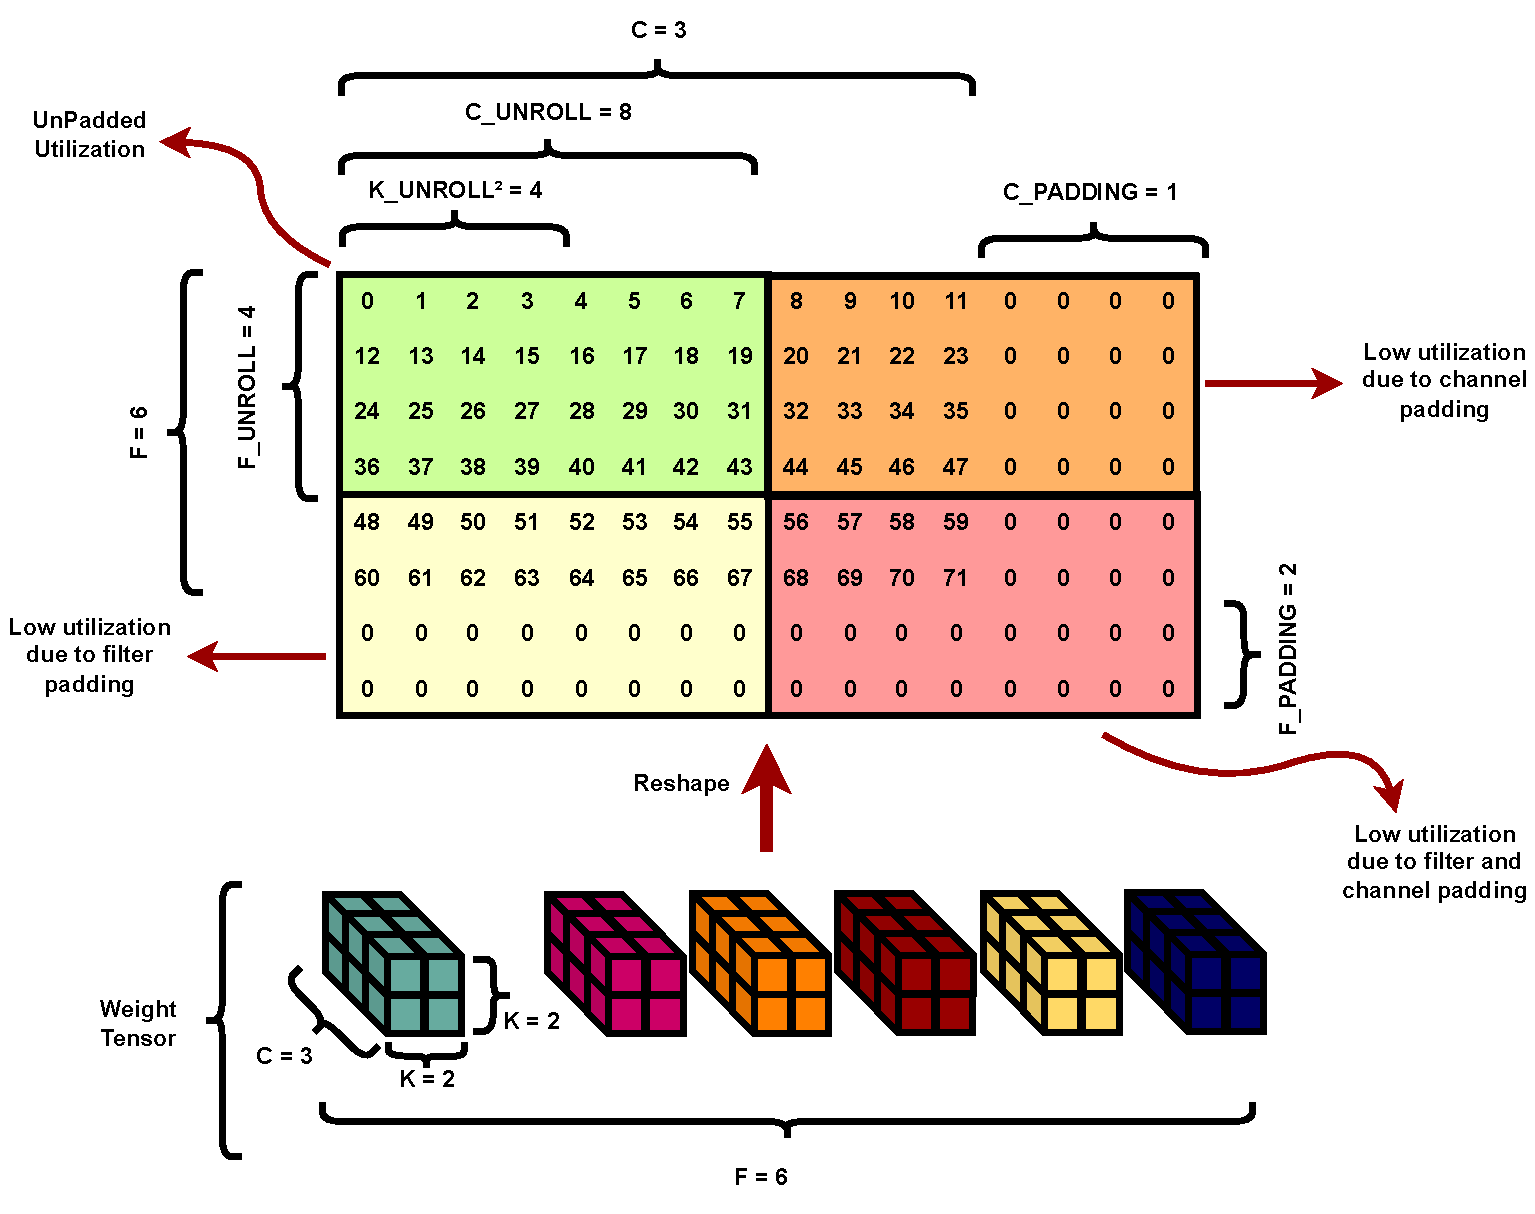
\includegraphics[scale=0.45]{fig/Lasso_ilus.pdf}
    \caption{\ac{GEMM} and 1x1 asd Equivelence}
    \label{fig:tempo_model}
\end{figure}

TEMPO models accelerator utilization based on how the template parameters (loop
unroll factors and loop axis mapping) tile and pad a convolution layer's
stationary weight tensor.  Kernel axis mapping is assumed to be inflexible
across accelerator spatial axis at runtime. An illustration of TEMPO's
utilization model in action is present in \autoref{fig:tempo_model}. In
\autoref{fig:tempo_model} a layer with a weight tensor of dimensionality
$R^{6\times 3\times 2\times 2}$ is tiled and padded based on the template
parameters $C_{unroll}=8$, $F_{unroll}=4$, $K_{unroll}=2$ and axis mapping
$K_{axis} = horizontal$. Based on these template parameters the effective filter
and channel unroll factors are $F_{eff} = 4$, $C_{eff}=2$. These unroll factors
create $\lceil \frac{\hat{C}}{C_{eff}} \rceil = 2$ horizontal tiles and $\lceil
\frac{\hat{F}}{F_{eff}} \rceil = 2$ verticle tiles assuming padding has been
applied. The weight tensor in \autoref{fig:tempo_model} is then reshaped into a
2D matrix of dimensionality $R^{8\times 16}$ with additional padding. The total
number of tiles is then reflected in \autoref{math:total_tiles}. 

\begin{align}
    \begin{gathered}
        Count_{Tiles} = \lceil \frac{\hat{F}}{F_{eff}} \rceil \lceil \frac{\hat{C}}{C_{eff}} \rceil
        \end{gathered}
    \label{math:total_tiles}
\end{align}

Utilization is calculated on a per-tile basis. There are two different types of
tiles, padded and unpadded, each with their own utilization calculation. Layer
utilization is then an average of the utilizations of each tile type weighted by
their frequency of occurence in the layer as reflect in
\autoref{math:layer_utilization}. For brevity each of the utilization equations
are multiplied by their frequency of occurence in the same equation. 

\begin{align}
    \begin{gathered}
        LayerUtilization = \frac{utilization^{UnPadded}_{Tiles} + utilization^{Padded}_{Tile(s)}}{Count_{Tiles}} \\
            \end{gathered}
    \label{math:layer_utilization}
\end{align}

The first tile type is the unpadded tile illustrated in
\autoref{fig:tempo_model} as the green tile. Utilization is calculated using
\autoref{math:tile_utilization_unpadded}. In this tile utilization is assumed to
be 1 and it's frequency of occurence depends on the number of unpadded tiles in
the layer $\lfloor \frac{\hat{F}}{F_{eff}} \rfloor \lfloor
\frac{\hat{C}}{C_{eff}}\rfloor$. 

\begin{align}
    \begin{gathered}
        utilization^{UnPadded}_{Tiles} = 1.\lfloor \frac{\hat{F}}{F_{eff}} \rfloor \lfloor \frac{\hat{C}}{C_{eff}}\rfloor \\
            \end{gathered}
    \label{math:tile_utilization_unpadded}
\end{align}

The second tile type is the padded tile of which there are three variations
depending on the reason for padding the tile. The utilization for all
padded tiles weighted by their frequencies of occurence is given in
\autoref{math:unpadded_tiles_weighted_average}. 

\begin{equation}
    \begin{aligned}
        utilization^{Padded}_{Tile(s)} & = utilization^{Padded}_{ChannelTiles} \\
                                       & + utilization^{Padded}_{FilterTiles} \\
                                       & + utilization^{Padded}_{ChannelAndFilterTiles} \\
    \end{aligned}
    \label{math:unpadded_tiles_weighted_average}
\end{equation}
  
If the allocation of PEs for channel loops exceeds avaliable channels to be
processed in the tile, then that tile will be padded. The padding in that tile results
in reduced PE utilization. An illustration of that padded tile variation is
present in \autoref{fig:tempo_model} as the orange tile.  The calculation for
the weighted utilization in that tile variation is given in equation
\autoref{math:tile_utilization_padded_channel}. To determine if a a padded channel
exists or not we can check if $\hat{C} \bmod C_{eff} > 0$ is true. If that
condition is true, padded channel tiles exist in the layer and their weighted
$utilization^{Padded}_{ChannelTiles}$ is then a function of how many PEs are
active in the tile $\frac{(\hat{C} \bmod C_{eff}) F_{eff}
K_{unroll}^2}{Count_{pe}}$ multipled by the frequency of occurence. $\lfloor
\frac{\hat{F}}{F_{eff}} \rfloor$. If $\hat{C} \bmod C_{eff} = 0$ then there are
no padded channel tiles so $utilization^{Padded}_{ChannelTiles} = 0$.

\begin{align}
    \begin{gathered}
        utilization^{Padded}_{ChannelTiles} = \begin{cases} \frac{(\hat{C} \bmod C_{eff}) F_{eff} K_{unroll}^2}{Count_{pe}}.\lfloor \frac{\hat{F}}{F_{eff}} \rfloor
         & \hat{C} \bmod C_{eff} > 0 \\ 0
         & \hat{C} \bmod C_{eff} = 0 \end{cases} \\
            \end{gathered}
    \label{math:tile_utilization_padded_channel}
\end{align}

If the allocation of PEs for filter loops exceeds avaliable filters to be
processed in the tile, then that tile will be padded. This another variation of
a padded tile and the weighted utilization for that tile variation is calculated
using \autoref{math:tile_utilization_padded_filter} and is illustrated in
\autoref{fig:tempo_model} as the yellow tile.

\begin{align}
    \begin{gathered}
        utilization^{Padded}_{FilterTiles} = \begin{cases} \frac{ C_{eff} (\hat{F} \bmod F_{eff}) K_{unroll}^2}{Count_{pe}}.\lfloor \frac{\hat{C}}{C_{eff}} \rfloor
            & \hat{F} \bmod F_{eff} > 0 \\ 0
            & \hat{F} \bmod F_{eff} = 0 \end{cases}
            \end{gathered}
    \label{math:tile_utilization_padded_filter}
\end{align}

Finally the last padded tile variation is the tile padded due to the excess
allocated of PEs for both filter and channel loops. This type of tile is
illustrated in \autoref{fig:tempo_model} as the red tile.  To determine if a tile like this
exists we can evaluate the condition $\hat{F} \bmod F_{eff} > 0 \land \hat{C}
\bmod C_{eff} > 0$ is true. If it there exists exactly one tile where
utilization is reduced due to excess allocation of PEs for filter and channel
loops. The equation to calculate weighted utilization in this padded tile
variation is given in \autoref{math:tile_utilization_padded_both}.

\begin{align}
    \begin{gathered}
         utilization^{Padded}_{Channel\&FilterTile} = \begin{cases} \frac{(\hat{C} \bmod C_{eff}) (\hat{F} \bmod F_{eff}) K_{unroll}^2}{Count_{pe}} & \hat{F} \bmod F_{eff} > 0 \land \hat{C} \bmod C_{eff} > 0 \\0  & else\end{cases}
            \end{gathered}
    \label{math:tile_utilization_padded_both}
\end{align}

\subsubsection{Metric: Latency}
\label{chap:dataflow_dse:exploring:tempo_model:latency}

Estimating latency follows the same tiling model discussed the previous
subsection. The latency of executing a layer based on the template paremeters
chosen is given in \autoref{math:latency}. Latency is a function of the number of
tiles present in the layer multiplied by the number of cycles spent processing a
single IFmap channel $\hat{Z}$ plus the additional latency incured due to
lowering lifting depending on the support for the layer's kernel size. Latency
for lowering and lifting is given in \autoref{math:latency_lowering_lifting}. If
the kernel is supported directly, no additional lowering and lifting penalties
are incurred, otherwise penalties are calculated based on the number of
operations necssary to lower the IFmap and Weight tensors plus the number of
operations to lift the OFmap. Lowering and lifting are assumed to be performed
by a software based co-processor. The latencies associated with lowering and
lifting can be eliminated if these operations are incoporated into the processor
however, that is left as part of future work. 

\begin{align}
    \begin{gathered}
        Latency = \hat{Z}.Count_{Tiles} + Latency_{Lowering} + Latency_{Lifting} \\
                \end{gathered}
    \label{math:latency}
\end{align}

\begin{align}
    \begin{gathered}
        Latency_{Lowering} = Latency_{Lifting} = \begin{cases} 0 &  K \in \{SupportedKernels\}\\ m^{2}K & K \notin \{SupportedKernels\}\end{cases} \\
                \end{gathered}
    \label{math:latency_lowering_lifting}
\end{align}

\subsubsection{Metric: Memory access counts}
\label{chap:dataflow_dse:exploring:tempo_model:access_counts}

Following the tiling model discussed earlier, memory access counts are
calculated based on how the template paremeters tile the layer's weight tensor.
Access counts for IFmaps are given in \autoref{math:memory_access_ifmap}, OFmap
access counts are giving in \autoref{math:memory_access_ofmap} and finally
weight access counts are given in \autoref{math:memory_access_weights}.

\begin{equation}
    \begin{aligned}
        IFmap^{AccessCount} = ((\hat{Z} K_{unroll}^2) (\lfloor\frac{\hat{C}}{C_{eff}} \rfloor C_{eff} + \hat{C}\bmod C_{eff}))\lceil\frac{\hat{F}}{F_{eff}}\rceil \\
    \end{aligned}
    \label{math:memory_access_ifmap}
\end{equation}
  
\begin{equation}
    \begin{aligned}
        OFmap^{AccessCount} = 2*\hat{Z} (\lfloor\frac{\hat{F}}{F_{eff}}\rfloor F_{eff}+\hat{F}\bmod F_{eff}) \lceil\frac{\hat{C}}{C_{eff}}\rceil \\
    \end{aligned}
    \label{math:memory_access_ofmap}
\end{equation}

\begin{equation}
    \begin{aligned}
        Weight^{AccessCount} & = \hat{Z}((C_{unroll}F_{unroll})(\lfloor\frac{\hat{C}}{C_{eff}} \rfloor \lfloor\frac{\hat{F}}{F_{Feff}}\rfloor) \\
            & +(C_{unroll}F_{eff})(\lfloor\frac{\hat{C}}{C_{eff}} \rfloor \hat{F}\bmod F_{eff}) \\
            & +(C_{eff}F_{unroll})(\lfloor\frac{\hat{F}}{F_{eff}} \rfloor \hat{C}\bmod C_{eff}) \\
            & + (C_{eff}F_{eff})(\hat{F}\bmod F_{eff}\space* \hat{C}\bmod C_{eff}))
        \end{aligned}
    \label{math:memory_access_weights}
\end{equation}

\subsection{TEMPO results}
\label{chap:dataflow_dse:exploring:results}

\subsubsection{Assumed objective function}
\label{chap:dataflow_dse:exploring:results:obj_fn}

Since TEMPO expects an objective function to maximize based on any or a
combination of all the discussed metrics in
\autoref{chap:dataflow_dse:exploring:tempo_model}
\autoref{math:tempo_results_obj_fn} defines an objective function based solely
on the average layer utilization metric over the entire set of convolution
layers in CIGAR's model library. Layer utilization is evaluated based on the
discussion in \autoref{chap:dataflow_dse:exploring:tempo_model:utilization}. 

\begin{equation}
        obj\_fn \gets average (\{LayerUtilization(layers)\space|\space \forall layers \in m, \forall m \in \{ModelLibrary\}\})
    \label{math:tempo_results_obj_fn}
\end{equation}

\begin{figure}[]
    \centering
    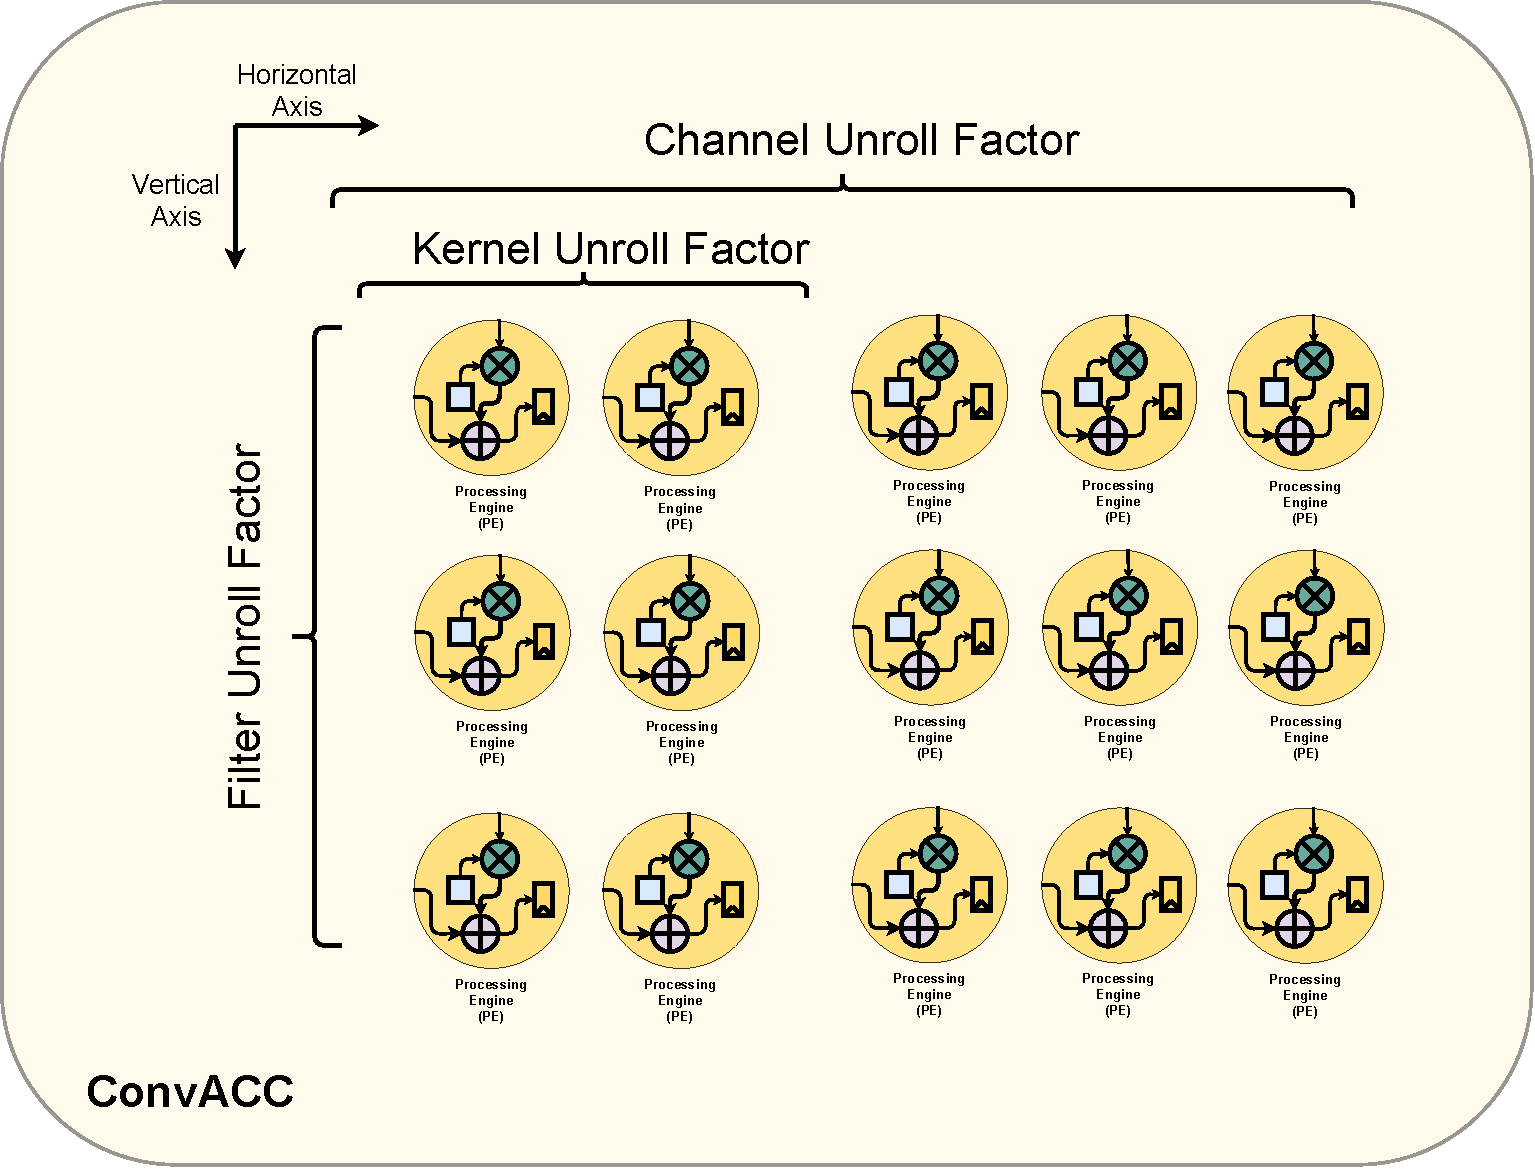
\includegraphics[scale=0.4]{fig/axis_mapping.pdf}
    \caption{\ac{GEMM} and 1x1 Convolution Equivelence}
    \label{fig:axis_mapping}
\end{figure}



% \State $arch_{config} \gets (f_{unroll}, c_{unroll}, k_{axis})$
% \For{$(model,\space layers) \in model^{stats}_{dict}$}
%     \For{$layer \in layers$}
%     \If{$layer.kernel\_size \notin kernels_{supported}$}
%         \State $\hat{layer} \gets supported\_layer\_equivelent(layer)$
%     \Else
%         \State $\hat{layer} \gets layer$
%     \EndIf
%     \State $layer_{metrics}.push (metrics\_fn(\hat{layer}, arch_{config}))$
%     \EndFor
% \EndFor 

% 
\chapter{Hardware Implementation design space exploration with the Polyhedral Model}
\label{chap:hw_dse:intro}

Based on the conclusion derived from \autoref{chap:dataflow_dse:intro},
the ideal conv. accelerator operates in two modes, direct Mode where 3x3 kernel
with stride 1 are supported and GEMM mode where all other kernel sizes and
strides are supported in GEMM mode via the approach in (REFERENCE LOWERING/
LIFTING CHAPTER). In this section we will deduce the optimal hardware
implementation for the weight stationary dataflow chosen in
\autoref{chap:dataflow_dse:intro} by analyzing data reuse in the loop based
representation of the aforementioned dataflow. To perform this deduction we will
use the polyhedral model to analyse temporal reuse in
\autoref{chap:hw_dse:temporal_analysis} and spatial reuse in
\autoref{chap:hw_dse:spatial_reuse_analysis}. Finally, in
\autoref{chap:hw_dse:simplifying_hierarchy} a simplification of the IFmap memory
hierarchy present in the optimal hardware implementation derived in
\autoref{chap:hw_dse:temporal_analysis} and
\autoref{chap:hw_dse:spatial_reuse_analysis} is presented.

\section{Temporal Reuse Analysis}
\label{chap:hw_dse:temporal_analysis}

Unrolling convolution dataflow loops yield multiple instances of the \ac{MAC}
statement present in the original convolution nested loops in
\autoref{lst:conv_loop}. These instances will be referred to as \ac{MAC} spatial
instances to distinguish them from temporal instances discussed in this chapter.
\ac{MAC} spatial instances can be distinguished based on the memory access
offsets that exist in them as a result of unrolling filter, channel and kernel
loops. For unroll factors F\_T for filters, C\_T for channels, KY\_T and KX\_T
for kernels each statement will have a coresponding access offset based on the
spatial instance index $j \in [0, F\_T*C\_T*KY\_T*KX\_T]$ for each of the data
elements (IFmap, OFmap and Weights) accessed in the loop body. Each \ac{MAC}
spatial instance at index j is characterized by a set of access offsets {Fj, Cj,
KYj, KXj} used by the memory accesses in the \ac{MAC} statement. Applying the
unroll factors and distinguishing each \ac{MAC} statement based on it's
statement index j yields the loop configuration in
\autoref{lst:conv_loops_unrolled}. 

\begin{lstlisting}[language=C, caption=Fully unrolled convolution dataflow loops, label={lst:conv_loops_unrolled}]
    for(int f = 0; f < F; f+=F_T) // Filter loop
        for(int c = 0; c < C; c+=C_T) // Channel loop
            for (int y = 0; y < Y; y++) // FeatureMap Height
                for(int x = 0; x < X; x++) // FeatureMap Width
                        ...
                        /* For all j in [0, F_T*C_T*KY_T*KX_T[ */ 
                        O[f+Fj][y][x] += W[f+Fj][c+Cj][KYj][KXj]* \
                                            I[c][y+KYj][x+KXj] 
                        ...
\end{lstlisting}

Temporal reuse analysis is performed on the above loops. The different
operational modes (GEMM/ Direct) are analysed concurrently using the same loop
representation below as they only differ based on whether we fuse feature map
height and width loops, and set upper bounds of the kernel loops to 1. Since
kernel loops are always unrolled fully this sets KY\_T and KX\_T to 1. We can
analyse temporal reuse in the dataflow represented in
\autoref{lst:conv_loops_unrolled} by adapting the approach in \cite{meeus} 
to the afformentioned dataflow iteration domain and access functions.
Given iteration domain restrictions imposed by the polyhedral model,
\autoref{lst:poly:analysis} assumes unroll factors F\_T =
C\_T = 4. Setting F\_T and C\_T to concrete values does not affect output
results of temporal reuse analysis.

\clearpage
\begin{lstlisting}[caption=Polyhedral analysis of reuse in iscc for convolution loops, label={lst:poly:analysis}]
    // Define iteration domain for all accessed data elements
    ID:=[F, C, Y, X] -> { S[f, c, y, x] : 0<=f<F and 0<=c<C and f mod 4=0 and c mod 4=0, 0<=y<Y and 0<=x<X};
    // Define access functions for each data element
    IFMAP:=([Cj, KYj, KXj] -> {S[f, c, y, x] -> IF[c+Cj][y+KYj][x+KXj]})*ID;
    OFMAP:=([Fj] -> {S[f, c, y, x] -> PS[f+Fj][y][x]})*ID;
    WEIGHT:=([Fj, Cj, KYj, KXj] -> {S[f, c, y, x] -> W[f+Fj][c+Cj][KYj][KXj]})*ID;
    // Evaluate temporal reuse
    IFMAP_REUSE:=(IFMAP.(IFMAP^-1))*(ID<<ID);
    OFMAP_REUSE:=(OFMAP.(OFMAP^-1))*(ID<<ID);
    WEIGHT_REUSE:=(WEIGHT.(WEIGHT^-1))*(ID<<ID);  

\end{lstlisting}

In \autoref{lst:poly:analysis}, the iteration domain for the loops in
\autoref{lst:conv_loops_unrolled} is converted into it's set representation in
line 2 where for some access statement S the loop iteration vector [f, c, y, x,]
is bound by the upper and lower bounds [0, F], [0, C], [0, Y], [0, X]
respectively. These bounds are represented by the associated parameters passed
to the iteration domain set assignment in line 2. Each memory accessed in the
body of the loop has an access function at each level of that memory's
hierarchy. As a result, each instance of the loop iteration vector [f, c, y, x]
is mapped to a memory access for each of the memories in lines 4-6. Access
offsets used in the memory access functions are passed as parameters based on
the convention established in \autoref{lst:conv_loops_unrolled}. This mapping
creates multiple temporal instances for each memory access in each \ac{MAC}
spatial instance.  For
example, for some iteration vector [f = 1, c = 1, y = 0, x = 1],
 the OFmap access that occurs at iteration vector [f = 2, c= 1, y = 0,
x = 1] is a different temporal instance of the same OFmap access at [f = 1, c = 1,
y = 0, x = 1]. 
Two accesses that access the same index but at different
iteration vectors are different temporal instances of the same access.
After applying the operation in lines 8-10, we can determine the
temporal reuse behavior of the accessed memories in the convolution loops.  
\autoref{lst:poly:result} shows the reuse behavior for each memory. Original
iteration domains constraints are ommited for brevity. 

\clearpage
\begin{lstlisting}[caption=Polyhedral analysis results w.r.t data elements in convolution loops, label={lst:poly:result}]
    IFMAP_REUSE;
    [F, C, Y, X, Cj, KYj, KXj]->{
        S[f, c, y, x] -> S[f', c' = c, y' = y, x' = x] :
            ... f' > f and 0 <= f' < F ... 
        }
    OFMAP_REUSE;
    [F, C, Y, X, Fj]->{ 
        S[f, c, y, x] -> S[f' = f, c', y' = y, x' = x] : 
            ... c' > c and 0 <= c' < C ... 
        }
    WEIGHT_REUSE;
    [F, C, Y, X, Fj, Cj, KYj, KXj] -> { 
        S[f, c, y, x] -> S[f' = f, c' = c, y', x'] : 
            ... y' > y and 0 <= y' < Y and 0 <= x' < X ...; 
    }
\end{lstlisting}

\autoref{lst:poly:result} shows the temporal reuse behavior in memory accesses. For each
of the memories accessed (IFmap, OFmap and Weights) there exists a set of reuse
(IFMAP\_REUSE, OFMAP\_REUSE and WEIGHT\_REUSE) maps that map each iteration
vector of an access to all the proceeding iteration vectors where that same
access occurs. From the above listing we can see that, in the set of IFmap reuse
maps (IFMAP\_REUSE), IFmap channels are reused temporally with respect to filter
loops. For a given IFmap accessed at channel c, that channel is accessed again
when computing the output for all proceeding filter loop iterationtions f' where
$f'>f$. The absence of other mappings in the set of reuse maps IFMAP\_REUSE shows
that 1) this reuse behavior holds at any arbitrary iteration vector [f, c, y, x]
and 2) this reuse behavior depends only on the filter loop. For the set OFmap
reuse maps (OFMAP\_REUSE), for an OFmap acceess at iteration vector [f, c, y,
x], it is accessed again at loop iteration f'=f, c', y'=y, x'=x where $c'>c$.  
For (WEIGHT\_REUSE) Weights exhibit temporal reuse w.r.t feature map width and
height, the X and Y loops. 

Applying the hardware taxonomy in \cite{maestro}, IFmap exhibits temporal reuse,
multicast communication. OFmap exhibits temporal reuse, reduction communication
given their read-modify-write behavior. Weights exhibit temporal multicast
communication. Given the limited implementation options derivable from temporal
reuse we can comfortably define the appropriate connectivity and memory
hierarchies for IFmaps channels, OFmaps channels (equivelent to number of
Filters), and Weights. The beginings of a hardware template derived from the
afformentioned temporal reuse behavior of the different memories referenced in
the convolution dataflow can be seen in \ref{fig:reuse_illus}. In
\ref{fig:reuse_illus} the template is broken into 3 major componenets. The first
is the IFmap memory hierarchy currently with only 1 level. The 2nd component is
the compute portion of the template where partial sums are computed and
aggregating into OFmap data elements. Finally the 3rd component which is the
OFmap memory that stores OFmap partial sums until they are aggregated into OFmap
pixels and are written back to memory.

\begin{figure}[]
    \centering
    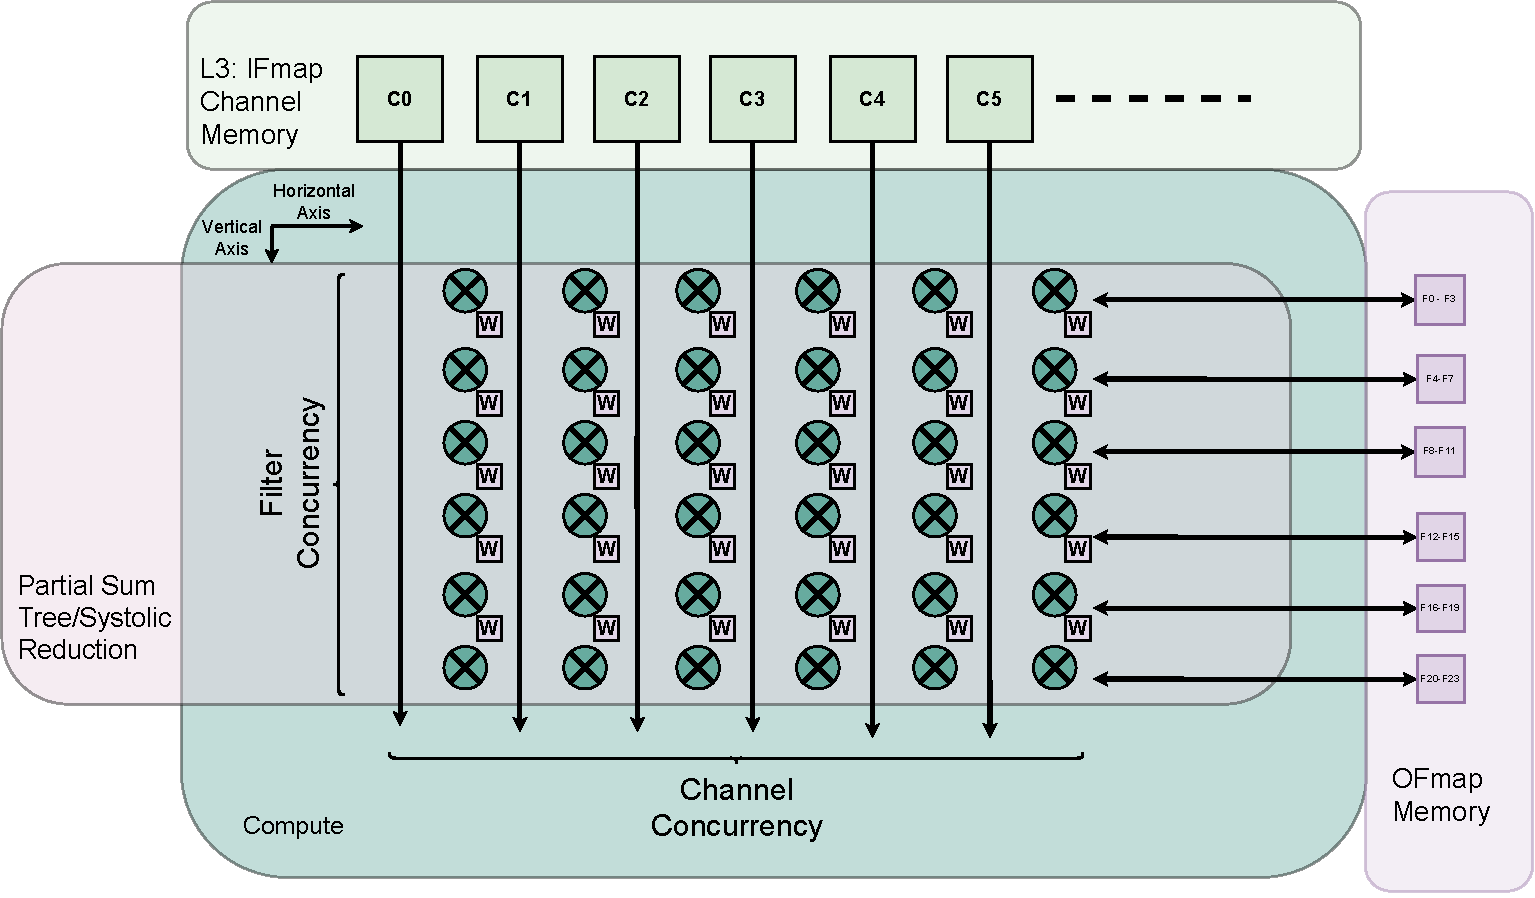
\includegraphics[scale=0.4]{fig/reuse_illus.pdf}
    \caption{Initial hardware template incorporating buffers IFmap and OFmap temporal reuse}
    \label{fig:reuse_illus}
\end{figure}

In addition to the temporal reuse behavior exhibited across IFmap channels,
temporal reuse exists within individual IFmap channels due to the stencil based
access pattern arising from the X, Y, KY, KX loops in the dataflow. That
temporal reuse is affected by the decision to fully unroll kernel loops which
causes temporal reuse to exist between unrolled IFmap kernel ports. Proof of the
existence of that temporal reuse is given in the polyhedral analysis in
\autoref{lst:poly:xy_reuse}. 

\begin{lstlisting}[caption=Analysis of IFmap channel reuse, label={lst:poly:xy_reuse}]
    ID_XY:=[Y, X, KY, KX] -> { S[y, x, ky, kx] : 0<=ky<KY and 0<=kx<KX and 0<=y<Y and 0<=x<X};
    IFMAP_XY:=({S[y, x, ky, kx] -> IF[y+ky][x+kx]})*ID;
    IFMAP_REUSE_XY:=(IFMAP_XY.(IFMAP_XY^-1))*(ID_XY<<ID_XY);
    IFMAP_XY_REUSE;
    [Y, X, KY, KX] -> { 
        S[y, x, ky, kx] -> S[y', x', ky' = (y - y') + ky, kx' = (x - x') + kx] : 
            ... y' > y and (y + ky) -KY < y' <= (y + ky) and (x + kx) -KX < x' <= (x + kx) ...;
    }
\end{lstlisting}

\begin{figure}[]
    \centering
    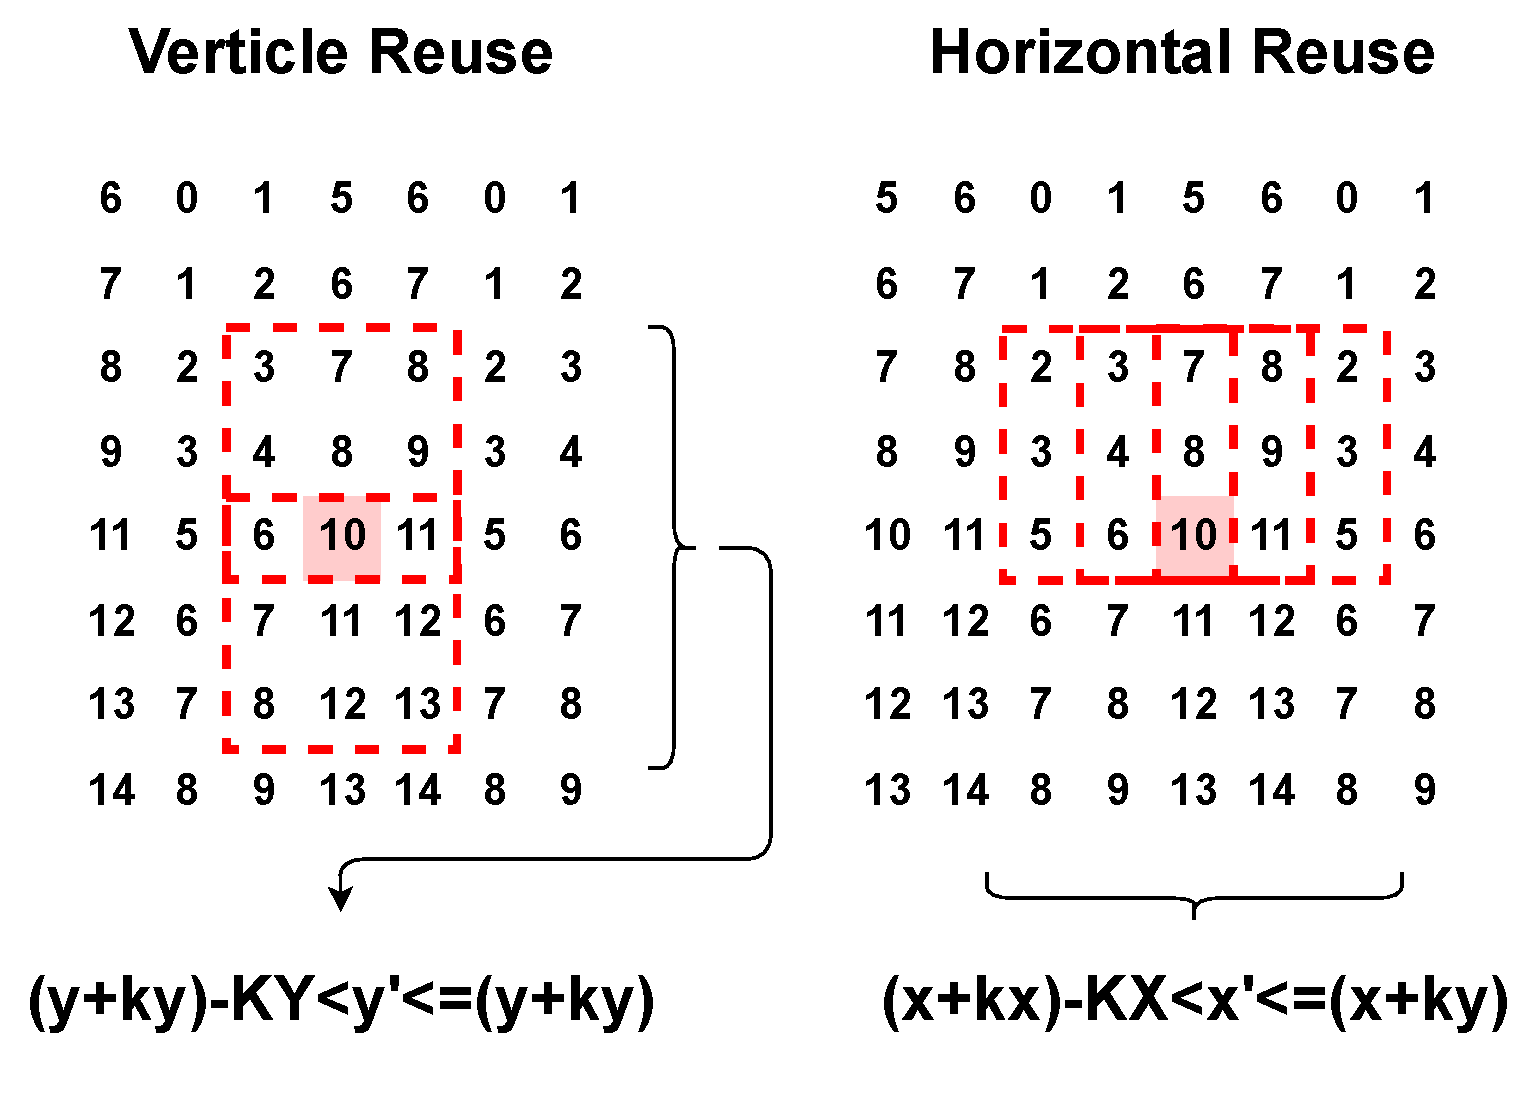
\includegraphics[scale=0.4]{fig/xy_reuse.pdf}
    \caption{IFmap Reuse Behavior w.r.t individual feature map channels}
    \label{fig:ifmap_xy_reuse}
\end{figure}

Within an individual IFmap channel, temporal reuse is exhibited w.r.t X and Y
loops. Given the complexity of the domain constraints of IFMAP\_XY\_REUSE in
\autoref{lst:poly:xy_reuse}, an illustration of the reuse behavior is available
in \figref{fig:ifmap_xy_reuse}. In \figref{fig:ifmap_xy_reuse}, individual
pixels within the kernel are reused based on the position of the sliding window
or stencil of the convolution in an IFmap channel. There are two primary
directions where that reuse is exhibited, vertical and horizontal with an IFmap
channel. The loops that control the verticle and horizontal stencil position in
the IFmap are the Y and X loops in the dataflow. Because kernel loops are fully
unrolled, the temporal reuse exhibited in \autoref{lst:poly:xy_reuse} occurs
accross unrolled kernel loop ports. To determine the appropriate memory
infrastructure to support that stencil based access pattern, we can apply the
technique in \cite{meeus} to construct a reuse chain that moves reused data
between urnolled kernel ports. The advantage of using a reuse chain is that the
temporal reuse that exists within an IFmap channel is relegated to a smaller
memory with lower memory access cost.

\cite{meeus} constructs a reuse chain for applications with a sliding window
access pattern that connects each unrolled kernel port with it's neighbors using
a FIFO or a shift register. If the temporal reuse distances between the accesses
of neighboring ports are constant \cite{meeus} uses a shift register, otherwise
they use a FIFO. The reuse distance between accesses of neighboring ports are
then converted into storage of the same size. So if two ports share the same
data but with a lag of 2 iterations in the iteration domain they're operating
in, then a shift register of size 2 can be placed between them. Similar to the
sliding window application explored in \cite{meeus} the reuse distances between
the unrolled kernel ports in the convolution dataflow are also constant. To
determine the reuse distances necessary between ports we can apply the analysis
in \autoref{lst:poly:xy_buffer_sizing:analysis} adapted from \cite{meeus} to
determine the sizing of the buffers in the reuse chain for IFmap accesses within
a channel. The analysis in \autoref{lst:poly:xy_buffer_sizing:analysis} assumes
a kernel size of 3x3. 


\begin{lstlisting}[caption=Determining buffer sizes in 3x3 convolutions, label={lst:poly:xy_buffer_sizing:analysis}]
    ID:=[IFMAP_Y, IFMAP_X] -> {S[y,x]:y>=0 and x>=0 and y<=IFMAP_Y-3 and x<=IFMAP_X-3};
    A0:=[IFMAP_Y, IFMAP_X] -> {S[y,x]->A[y+0,x+0]}*ID;
    A1:=[IFMAP_Y, IFMAP_X] -> {S[y,x]->A[y+0,x+1]}*ID;
    A2:=[IFMAP_Y, IFMAP_X] -> {S[y,x]->A[y+0,x+2]}*ID;
    A3:=[IFMAP_Y, IFMAP_X] -> {S[y,x]->A[y+1,x+0]}*ID;
    ...
    A8:=[IFMAP_Y, IFMAP_X] -> {S[y,x]->A[y+2,x+2]}*ID;

    R10:=(lexmin ((A1.A0^-1)*(ID<<ID)));
    R21:=(lexmin ((A2.A1^-1)*(ID<<ID)));
    R32:=(lexmin ((A3.A2^-1)*(ID<<ID)));
    ...
    R87:=(lexmin ((A8.A7^-1)*(ID<<ID)));
\end{lstlisting}

In \autoref{lst:poly:xy_buffer_sizing:analysis}, the iteration domain for the YX
loops are defined as functions of the IFmap dimensions passed as parameters (line 1).
The unrolled kernel loop IFmap accesses are then described using access maps
that map the iteration vector [y,x] to the associated IFmap access (lines 2-7).
Notice that the accesses are described as constant offsets added to access iterators y
and x. These constants represent the kernel loop iterators ky, and kx that are now
unrolled. For each neighboring pair of ports accessing the IFmap we can
determine the reuse behavior in (lines 9-10). Operations in lines (9-13) map
iterations where a port accesses a data element in IFmap with the earliest next
iteration in which the neighboring port accesses that same data element. The
distance between the accesses is then used as the reuse buffer size. The results
of the analysis are presented in \autoref{lst:poly:xy_buffer_sizing:results}.

\clearpage 

\begin{lstlisting}[caption=Polyhedral analysis of reuse in iscc for convolution loops, label={lst:poly:xy_buffer_sizing:results}]
R10;
$1 := [IFMAP_Y, IFMAP_X] -> { 
    S[y, x] -> S[y' = y, x' = 1 + x] : 
        0 <= y <= -3 + IFMAP_Y and 0 <= x <= -4 + IFMAP_X 
}
R21;
$2 := [IFMAP_Y, IFMAP_X] -> { 
    S[y, x] -> S[y' = y, x' = 1 + x] : 
        0 <= y <= -3 + IFMAP_Y and 0 <= x <= -4 + IFMAP_X 
}
R32;
$3 := [IFMAP_Y, IFMAP_X] -> { 
    S[y, x] -> S[y' = 1 + y, x' = -2 + x] : 
        0 <= y <= -4 + IFMAP_Y and 2 <= x <= -3 + IFMAP_X 
}
...
R87;
$8 := [IFMAP_Y, IFMAP_X] -> { 
    S[y, x] -> S[y' = y, x' = 1 + x] : 
        0 <= y <= -3 + IFMAP_Y and 0 <= x <= -4 + IFMAP_X 
}
\end{lstlisting}

In \ref{lst:poly:xy_buffer_sizing:results}, reuse distances between neighboring
ports depend on the relationship between the ports and whether their access offsets
are in the same row of the stencil or not. If two neighboring ports have unequal
ky offsets the reuse distance between them is IFMAP\_X-3. If two neighboring
ports have an equal ky offset the reuse distance is 1. An example of the first
case is lines 11-15 where the reuse distance between port 2 and port 3 is
IFmap-3. The evidence of that is that for any data accessed at port 3 with
iteration vector y, x that same data is accessed at port 2 at iteration vector
[y+1, x-2]. Based on the lexicographic ordering of iteration vector [y, x] and [y+1,
x-2], the distance between those two vectors is IFMAP\_X-3, or in terms of OFmap
dimensions X-1. Applying the same analysis to two ports in the same row (R10,
R21, R45, R87, ...) yields a reuse distance of 1 as evidence by the iteration
vectors of access [y, x] and [y, x+1] in all of the afformentioned neighboring
port pairs. 

Applying the results of the analysis in
\autoref{lst:poly:xy_buffer_sizing:results} with the previous template \autoref{fig:reuse_illus}
results in the updated template \autoref{fig:reuse_chain}.

\begin{figure}[]
    \centering
    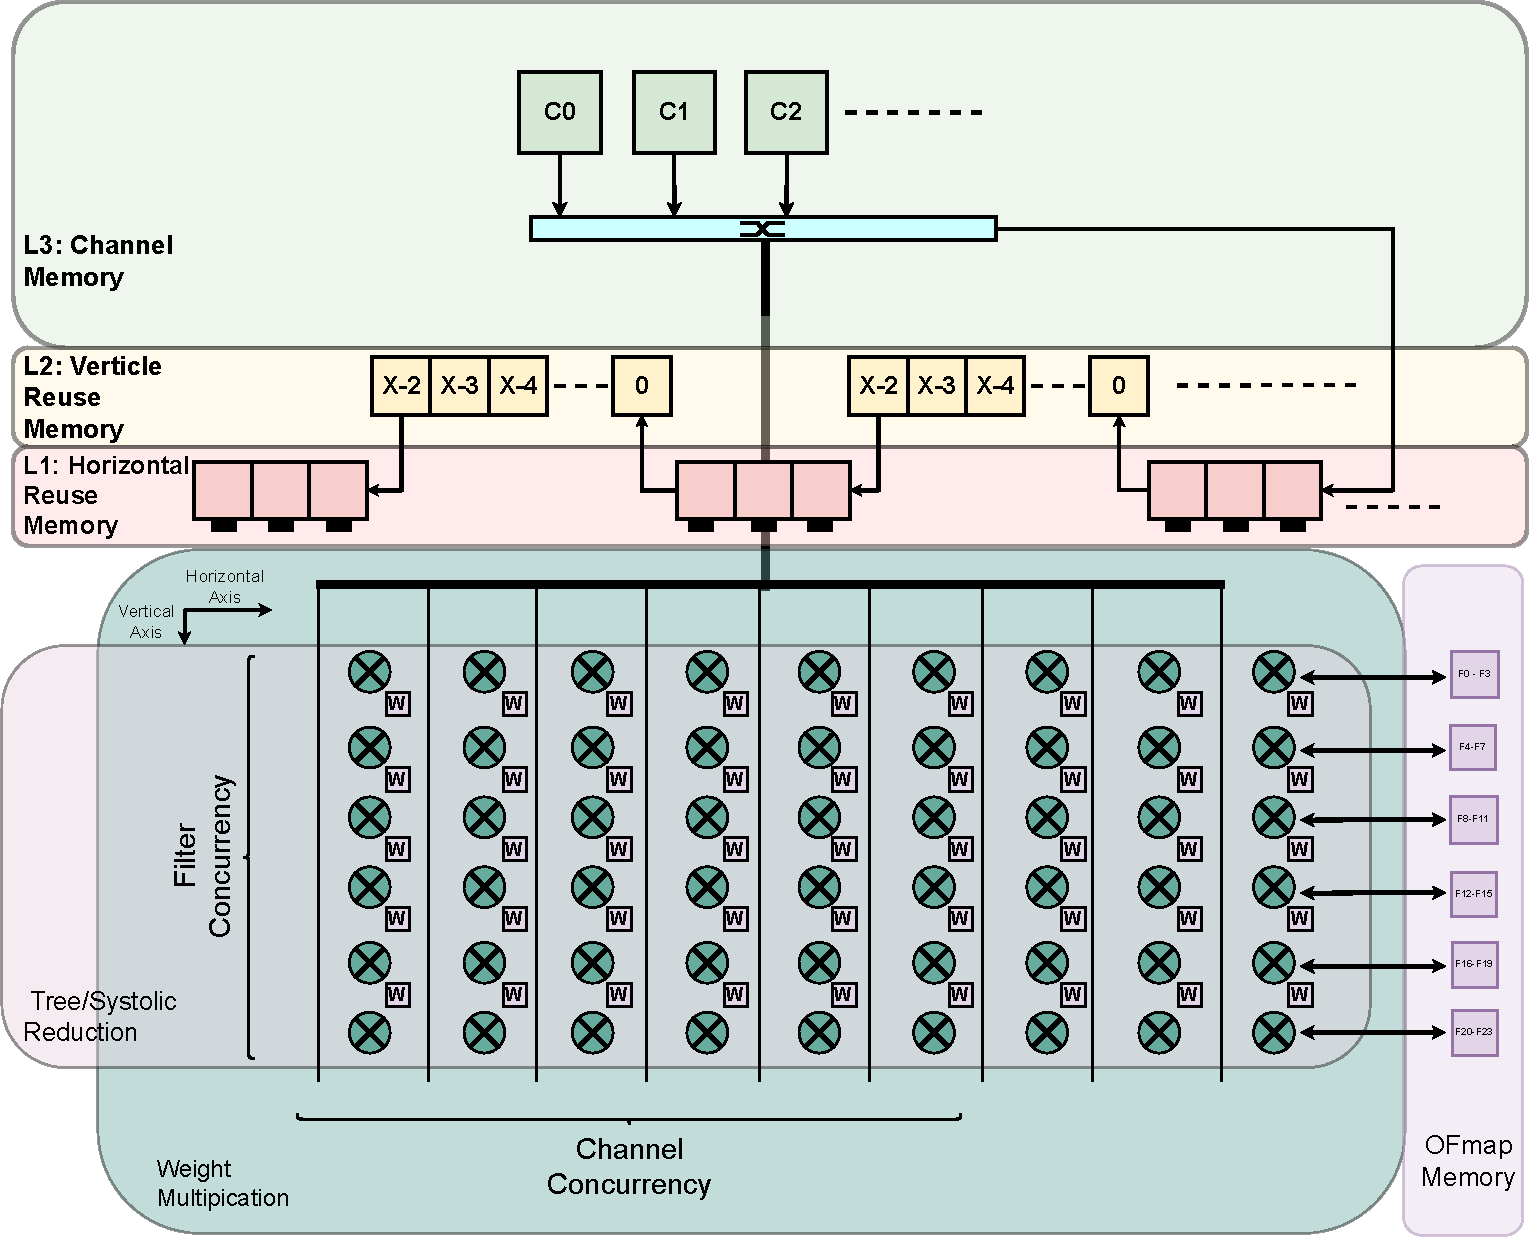
\includegraphics[scale=0.4]{fig/reuse_chain.pdf}
    \caption{Hardware template incorporating a reuse chain for reuse within an IFmap channel }
    \label{fig:reuse_chain}
\end{figure}


\section{Spatial Reuse Analysis}
\label{chap:hw_dse:spatial_reuse_analysis}

So now we know the hierarchy needed to express X and Y reuse in IFmap. Applying
the unroll factors in the target loops in the dataflow will yield a loop
structure similar to the one in \ref{lst:conv_loops_unrolled_fully}. Using the
convention established in \ref{chap:hw_dse:temporal_analysis}, each
\ac{MAC} statement in the unrolled loop body has an associated j index. In the
loop body there exists duplicate memory accesses across individual \ac{MAC}
spatial instances. Those duplicate accesses are highlighted in
\autoref{lst:conv_loops_unrolled_fully} and they are the origin of spatial reuse
in the dataflow. IFmaps exhibit spatial reuse with multicast communication w.r.t
to filter loops. OFmap exhibit spatial reuse with reduction communication
w.r.t to channel loops. Weights exhibit no spatial reuse 
 
\clearpage
\begin{lstlisting}[language=C, caption=Spatial reuse in fully unrolled kernel loops, label={lst:conv_loops_unrolled_fully}]
for(int f = 0; f < F; f+=F_T) // Filter loop
    for(int c = 0; c < C; c+=C_T) // Channel loop
        for (int y = 0; y < Y; y++) // FeatureMap Height
            for(int x = 0; x < X; x++) // FeatureMap Width
            {
                %\colorbox{green}{O[f+0][y][x]}% += W[f+0][c+0][0][0] * \ 
                                    %\colorbox{yellow}{I[c+0][y+0][x+0]}%; // j=0
                %\colorbox{green}{O[f+0][y][x]}% += W[f+0][c+0][0][1] * \
                                    %\colorbox{yellow}{I[c+0][y+0][x+1]}%; // j=1
                %\colorbox{green}{O[f+0][y][x]}% += W[f+0][c+0][0][2] * \
                                    I[c+0][y+0][x+2];  // j=2
                %\colorbox{green}{O[f+0][y][x]}% += W[f+0][c+0][1][0] * \ 
                                    I[c+0][y+1][x+2];  // j=3
                ...
                %\colorbox{red}{O[f+1][y][x]}% += W[f+1][c+0][0][0] * \
                                    %\colorbox{yellow}{I[c+0][y+0][x+0]}%; // j=C_T*KY_T*KX_T
                %\colorbox{red}{O[f+1][y][x]}% += W[f+1][c+1][0][1] * \
                                    %\colorbox{yellow}{I[c+0][y+0][x+1]}%; // j=C_T*KY_T*KX_T+1
                ...
                O[f+F_T-1][y][x] += W[f+F_T-1][c+C_T-1][KY_T-1][KX_T-1] * \ 
                                        I[c][y+KY_T-1][x+KX_T-1]; 
                                                    // j=F_T*C_T*KY_T*KX_T-1
                                        
            }
\end{lstlisting}

Applying the taxonomy in \autoref{fig:hw_taxonomy} to data elements that are
spatially reused, IFmap channels that are spatially reused across unrolled
filter loops can be broadcast with a bus. The reuse chain discussed in
\autoref{chap:hw_dse:temporal_analysis} can be thought of as a
Store\&Forward scheme to deliver individual IFmap channel data elements to the
\ac{PE}s for reduction into OFmaps.Weights reused for channel iteration and are
discarded. They exhibit no spatial reuse, just temporal. Therefore they should
be kept in small on chip buffers, preferably close to the computation they are
used in. OFmap exhibit spatial reuse across concurrent channels as well as
temporal reuse across channel sets as discussed in
\autoref{chap:hw_dse:temporal_analysis}. A reduction tree as in
\autoref{fig:reduction_styles}.a or a systolic array reduce and fwd as in
\autoref{fig:reduction_styles}.b are both possible assuming no restrictions
arising from synthesis. Combining the reuse chain derived in
\autoref{chap:hw_dse:temporal_analysis} with the required systolic
delays yields a simplification to the L1 memory present in
\autoref{fig:reuse_chain}. This simplification is discussed in
\autoref{chap:hw_dse:simplifying_hierarchy}.


\begin{figure}
    \centering
    \subfigure[]{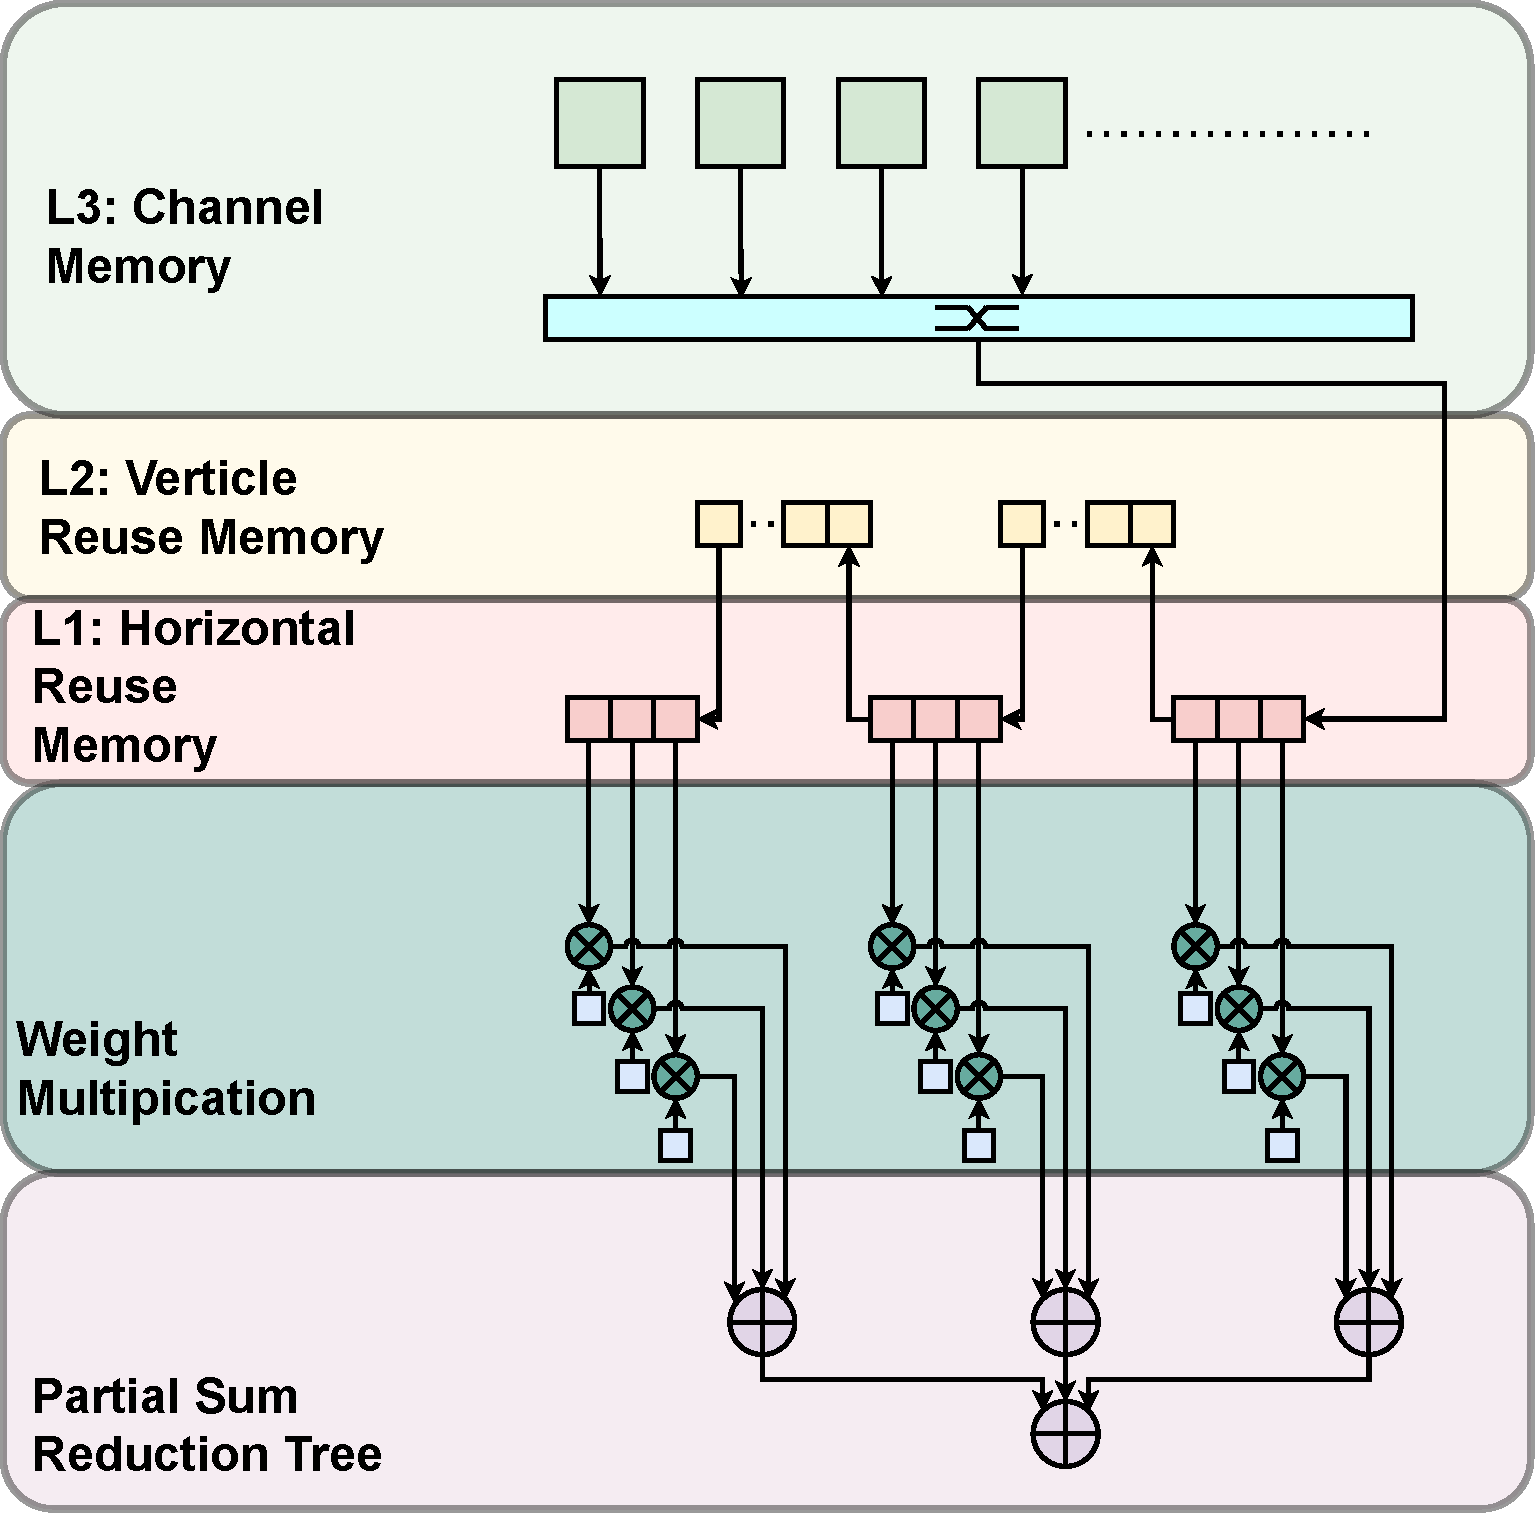
\includegraphics[width=0.5\textwidth]{fig/treeReduction.pdf}}
    \subfigure[]{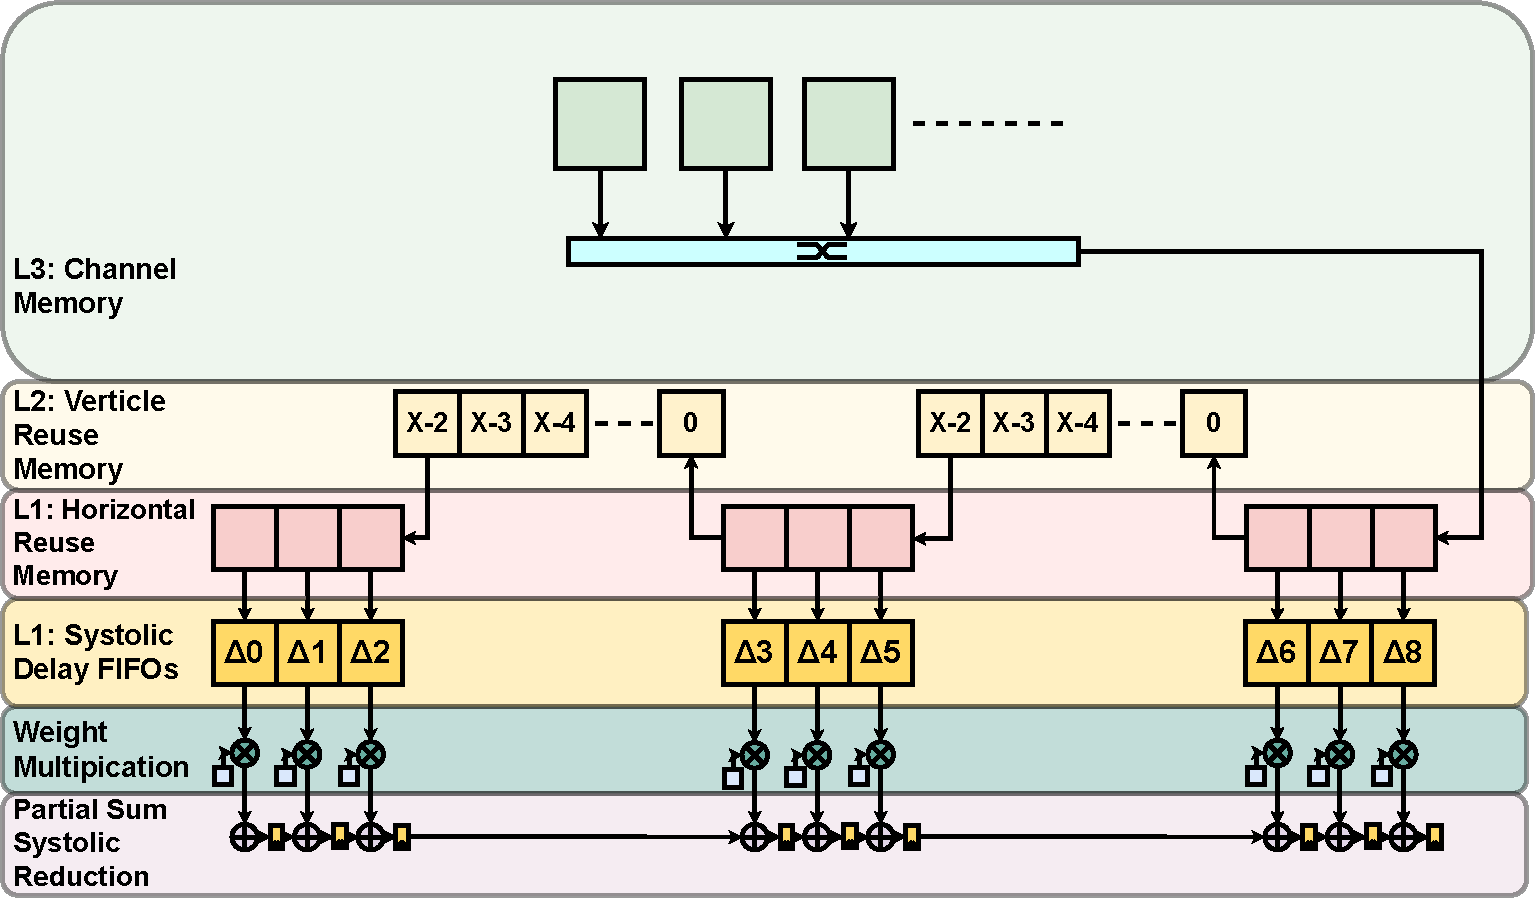
\includegraphics[width=0.7\textwidth]{fig/SystolicReduction.pdf}}
    \caption{Illustration of different partial sum reduction styles assuming kernel size is 3x3 (a) Tree Reduction (b) Systolic array reduction}
    \label{fig:reduction_styles}
\end{figure}

\section{Simplifying the memory hierarchy}
\label{chap:hw_dse:simplifying_hierarchy}

\begin{figure}[]
    \centering
    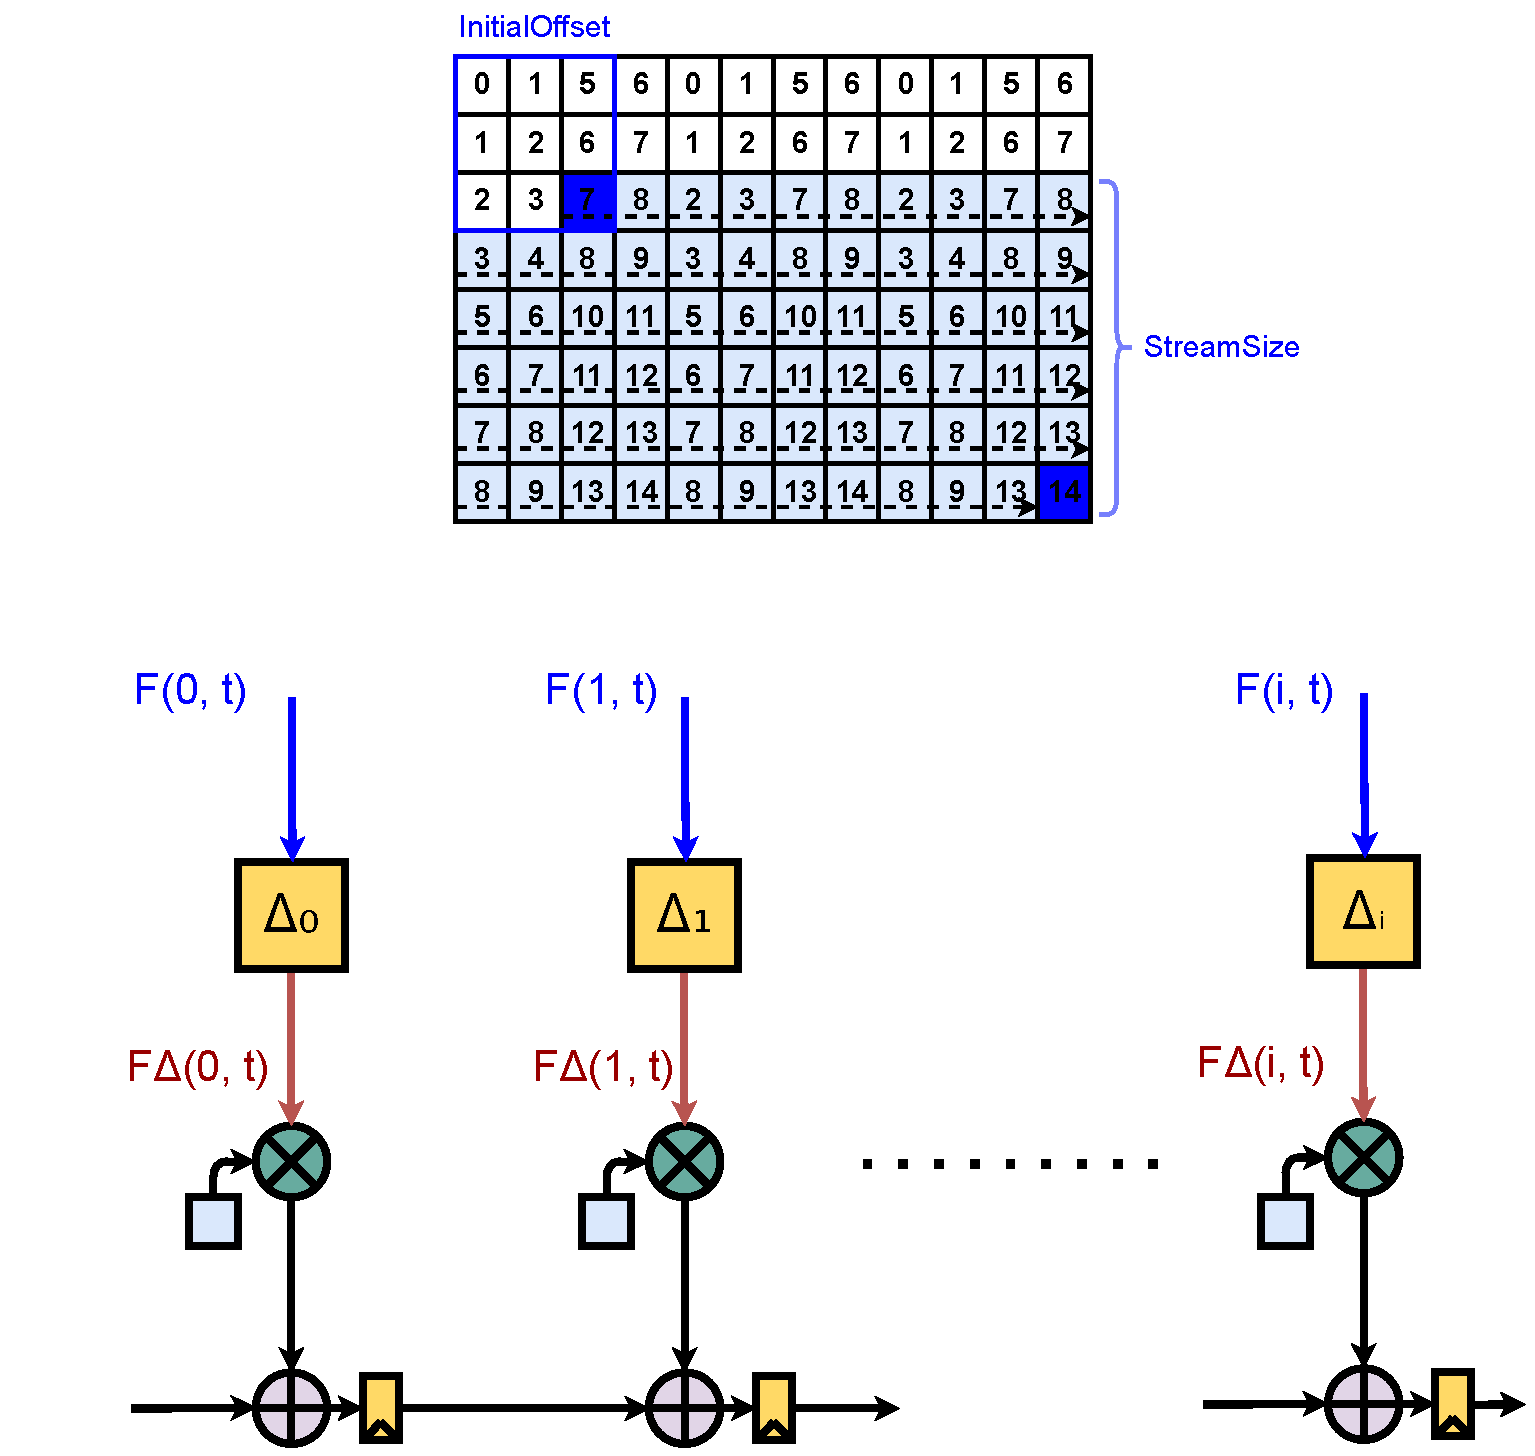
\includegraphics[scale=0.5]{fig/delayproof.pdf}
    \caption{Reinterpretation of IFmap memory hierarchy outputs as a stream function}
    \label{fig:delay_proof}
\end{figure}

We can reinterpret the accesses made by the IFmap memory hierarchy in
\autoref{fig:reuse_chain} as a stream function $F(i, t)$ whose output produces
element from an IFmap channel. The variable $i$ is the port index of IFmap
hierarchy and $t$ is the time in cycles since the beginning of the convolution
operation. A representation of this reinterpretation of the accesses made in the
IFmap memory hierarchy can be seen in \autoref{fig:delay_proof}. Since it's
always assumed that in direct mode kernel loops are unrolled fully the number of
ports into the IFmap memory hierarchy is always a multiple of $K^2$ where $K$ is
the size of the kernel being processed in direct mode. 

\begin{gather}
    IFmap \in R^{C\times n \times n} \xrightarrow{Reshape} IFmap \in R^{1\times Cn^2} \\
    Weight \in R^{F\times C\times K \times K} \\
    F(i, t)=    \begin{cases}
                    IFmap_{A(i, t)} & 0<=t < StreamSize \\
                    0 & else
                \end{cases} \\
    StreamSize = n(n-K)+(n-K) \\
    A(i, t) = InitialOffset(i) + t\\
\end{gather}

Each data element streamed from the IFmap depends on the an access function that
also takes the same variables $i$ and $t$. Depending on the port index $i$ the
access function for each port is composed on an initial offset in the IFmap and
the current cycle count. The number of cycles in which output from the IFmap
memory hierarchy can be produced is limited to the stream size of the IFmap
currently being processed. The stream size is a function of the IFmap dimensions
and the kernel Size. 

\begin{gather}
    InitialOffset = C_in^2+Y_in+X_i \\
    C_i = \lfloor \frac{\lfloor \frac{i}{K} \rfloor}{K} \rfloor \\
    Y_i = (\lfloor \frac{i}{K} \rfloor ) \bmod K\\
    X_i = i \bmod K = (i - \lfloor \frac{i}{K} \rfloor K)\\
\end{gather}

The initial offset function defines the initial index
offset in the IFmap the stream starts from for each port $i$. It can be
decomposed into three main offsets. A channel offset $C_i$, a row offset $Y_i$
and a column offset $X_i$. 

\begin{gather}
    F_\Delta(i, t) = \begin{cases}
    IFmap_{A_\Delta(i, t)} & \Delta_i<=t < \Delta_i+ StreamSize \\
    0 & else
    \end{cases} \\
    \Delta_i = i \\
    A_\Delta(i,t) = A(i, t) - \Delta_i\\
    % \hat{OFmap}(j) = \displaystyle\sum\limits_{i=0}^{ub(i)} A_\Delta(i, j+i)
\end{gather}

Under this new streaming based interpretation of the accesses in the IFmap
memory hierarchy, the delay elements in the systolic reduction scheme in
\autoref{fig:reduction_styles}.b are represented as time shifts in the stream
function $F(i,t)$. These time shifts are represented in the new delayed access
function $A_\Delta(i, t)$.

\begin{gather}
    A_\Delta(i,t) =  C_in^2+Y_in+(i - \lfloor \frac{i}{K} \rfloor K) + t- i\\
    A_\Delta(i,t) =  \lfloor \frac{\lfloor \frac{i}{K} \rfloor}{K} \rfloor^2+(\lfloor \frac{i}{K} \rfloor ) \bmod K + \underbrace{(- \lfloor \frac{i}{K} \rfloor K)}_{X'_i} + t\\
    % \hat{OFmap}(j) = \displaystyle\sum\limits_{i=0}^{ub(i)} A_\Delta(i, j+i)
\end{gather}

\begin{figure}[]
    \centering
    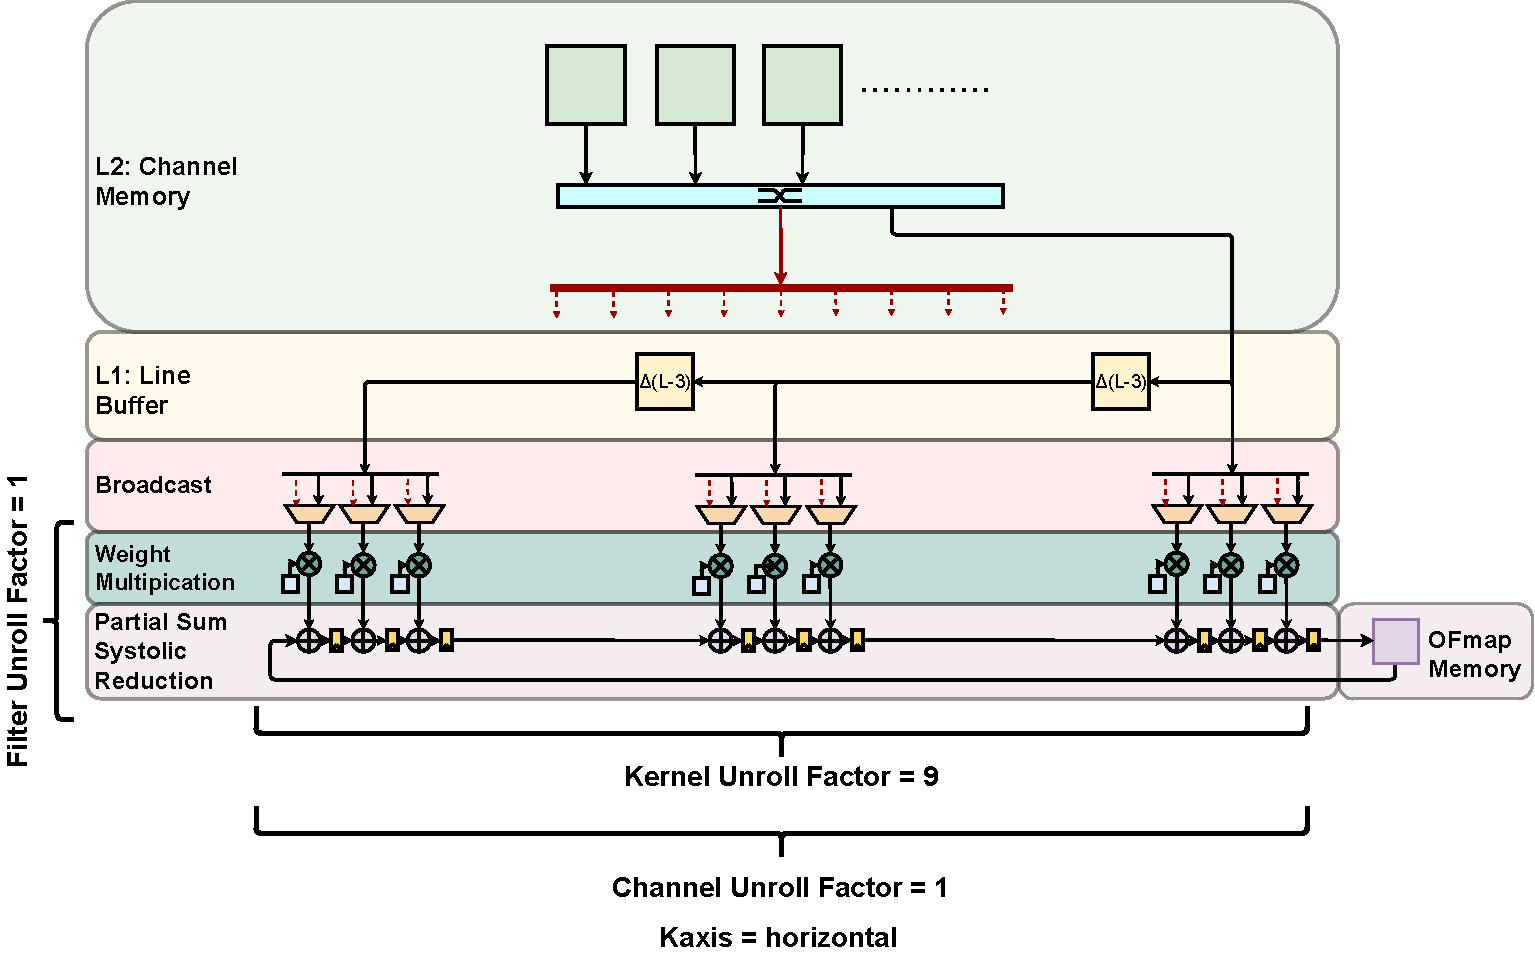
\includegraphics[scale=0.36]{fig/hybrid3x3Gemm.pdf}
    \caption{Using a systolic reduce and forward to calculate OFmaps}
    \label{fig:simplified_systolic_reduction}
\end{figure}

Substituting the InitialOffset function in $A_\Delta$  allows us to simplify the
column offset. This yields a new column offset $X'_i$. The final delayed access
function's initial offset becomes insensitive to changes in the port index $i$
that are not multiples of $K$. This allows us to remove the lowest layer memory
along with the systolic array delays in \autoref{fig:reuse_chain} and replace
both layers with just a series of broadcast buses that span consecutive $K$
groups of IFmap ports provided that we relax the start time constraints to the
$\lceil \frac{i}{K} \rceil$ for each group of ports $\lfloor \frac{i}{K}
\rfloor$. Delays in accessing IFmap data elements accross $K$ groups of ports
as well as accross $K^2$ groups of ports accessing different channels still
remain. This simplifying the hierarchy by removing the systolic delays thus still
requiring complex delayed reads from the IFmap hierarchy which necessitates smart
SRAMS whose access times can be programmed. A discussion of these smart memories
is presented in \autoref{chap:acc_sched:primitives:da-sram}. The final
hardware implementation with the added IFmap memory hierarchy optimization
discussed in this section is given in
\autoref{fig:simplified_systolic_reduction}.
\autoref{fig:simplified_systolic_reduction} shows the broadcast busses for every
group of 3 processing engines as well as the 1x1 vertical broadcast busses
highlighted in red. 


% https://www.desmos.com/calculator/y0oszemsuo

% Under 3x3/1x1 Direct Highest level ifmap. Layer size graph, ub 2\^19 bytes
% covers 95\% of networks. This leads to small area size (reference Jinghan paper)
% Does not scale with systolic array size. PSUM storage, depends on tiling
% schedule. Reference WC and psum storage scaling graph. WC equal to layer size
% graph ub. Scales with systolic array. Weights are reused then discarded for one
% inference pass. Double buffer and stream from memory. If model size is small
% enough/ sparsity is taken advantage of, we can store the weights on chip.
% However, this was not considered in this work. 

% GEMM mode im2col not only way of reshaping data. im2col maximizes bloat for
% ifmap. Solution is less bloaty im2col. Max storage required will be less 2\^19
% with balanced lifting and lowering. This implies that CPU has to do some vector
% ops concurrently with accelerator or vector ops should be added to accelerator.
% This not considered in this work.  

% moving on to memory scalability
% ifmap memory, we need 2\^19 bytes to support 95\% of networks
% layers that exceed that size are assumed to be too large
% we can trade off ifmap memory with psum memory if we switch loop ordering
% (show trade off graph), F, C is ASAP, C, F is alap. under asap
% psum storage scales with F, under alap max number of ofmaps are 
% in flight so that maximizes psum storage but we only need to keep 
% C worth of tiles in flight

% weight storage scales with the size of the systolic array

% GEMM_ID:=[F, C, Z] -> { S[f,c,z] : 0<=f<F and  0<=c<C and 0<=z<Z and f%4=0 and c%4=0};
% GEMM_IFMAP:=([F, C, Z, ci] -> {S[f,c,z] -> IF[c+ci][z]})*GEMM_ID;
% GEMM_IFMAP_REUSE:=(GEMM_IFMAP.(GEMM_IFMAP^-1))*(GEMM_ID<<GEMM_ID);
% GEMM_PSUM:=([F, C, Z, fi] -> {S[f,c,z] -> PS[f+fi][z]})*GEMM_ID;
% GEMM_PSUM_REUSE:=(GEMM_PSUM.(GEMM_PSUM^-1))*(GEMM_ID<<GEMM_ID);
% GEMM_WEIGHT:=([F, C, Z, fi, ci] -> {S[f,c,z] -> W[f+fi][c+ci]})*GEMM_ID;
% GEMM_WEIGHT_REUSE:=(GEMM_WEIGHT.(GEMM_WEIGHT^-1))*(GEMM_ID<<GEMM_ID);


% DIRECT_ID:=[F, C, Y, X] -> { S[f,c,y,x] : 0<=f<F and 0<=c<C and 0<=y<Yth
% and 0<=x<X and f%4=0 and c%4=0};
% DIRECT_IFMAP:=([F, C, Y, X, ci, ky, kx] -> {S[f,c,y,x] -> IF[c+ci][y+ky][x+kx]})*DIRECT_ID;
% DIRECT_IFMAP_REUSE:=(DIRECT_IFMAP.(DIRECT_IFMAP^-1))*(DIRECT_ID<<DIRECT_ID);
% DIRECT_PSUM:=([F, C, Y, X, fi] -> {S[f,c,y,x] -> PS[f+fi][y][x]})*DIRECT_ID;
% DIRECT_PSUM_REUSE:=(DIRECT_PSUM.(DIRECT_PSUM^-1))*(DIRECT_ID<<DIRECT_ID);
% DIRECT_WEIGHT:=([F, C, Y, X, fi, ci, ky, kx] -> {S[f,c,y,x] -> W[f+fi][c+ci][ky][kx]})*DIRECT_ID;
% DIRECT_WEIGHT_REUSE:=(DIRECT_WEIGHT.(DIRECT_WEIGHT^-1))*(DIRECT_ID<<DIRECT_ID);


% YX_ID:=[Y, X, KY, KX] -> { S[y, x, ky, kx] : 0<=y<Y and 0<=x<X and 0<=ky<KY and 0<=kx<KX};
% YX_IFMAP:=([Y, X, KY, KX] -> {S[y, x, ky, kx] -> IF[y+ky][x+kx]})*DIRECT_KERNEL_ID;
% YX_IFMAP_REUSE:=(DIRECT_KERNEL_IFMAP.(DIRECT_KERNEL_IFMAP^-1))*(DIRECT_KERNEL_ID<<DIRECT_KERNEL_ID);
% YX_PSUM:=([Y, X, KY, KX] -> {S[y, x, ky, kx] -> PS[y][x]})*DIRECT_KERNEL_ID;
% YX_PSUM_REUSE:=(DIRECT_KERNEL_PSUM.(DIRECT_KERNEL_PSUM^-1))*(DIRECT_KERNEL_ID<<DIRECT_KERNEL_ID);
% YX_WEIGHT:=([Y, X, KY, KX] -> {S[y, x, ky, kx] -> W[ky][kx]})*DIRECT_KERNEL_ID;
% YX_WEIGHT_REUSE:=(DIRECT_KERNEL_WEIGHT.(DIRECT_KERNEL_WEIGHT^-1))*(DIRECT_KERNEL_ID<<DIRECT_KERNEL_ID);

% Reuse w.r.t F and C loops


% RDIST_R10:=ub(card(((R10^-1).(ID<<=ID)*(ID<<=ID)^-1).A0));
% RDIST_R21:=ub(card(((R21^-1).(ID<<=ID)*(ID<<=ID)^-1).A1));
% RDIST_R32:=ub(card((*(ID<<=ID)^-1).A2));
% RDIST_R43:=ub(card(((R43^-1).(ID<<=ID)*(ID<<=ID)^-1).A3));
% RDIST_R54:=ub(card(((R54^-1).(ID<<=ID)*(ID<<=ID)^-1).A4));
% RDIST_R65:=ub(card(((R65^-1).(ID<<=ID)*(ID<<=ID)^-1).A5));
% RDIST_R76:=ub(card(((R76^-1).(ID<<=ID)*(ID<<=ID)^-1).A6));
% RDIST_R87:=ub(card(((R87^-1).(ID<<=ID)*(ID<<=ID)^-1).A7));


% R43;
% $4 := [IFMAP_Y, IFMAP_X] -> { 
%     S[y, x] -> S[y' = y, x' = 1 + x] : 
%         0 <= y <= -3 + IFMAP_Y and 0 <= x <= -4 + IFMAP_X 
% }
% R54;
% $5 := [IFMAP_Y, IFMAP_X] -> { 
%     S[y, x] -> S[y' = y, x' = 1 + x] : 
%         0 <= y <= -3 + IFMAP_Y and 0 <= x <= -4 + IFMAP_X 
% }
% R65;
% $6 := [IFMAP_Y, IFMAP_X] -> { 
%     S[y, x] -> S[y' = 1 + y, x' = -2 + x] : 
%         0 <= y <= -4 + IFMAP_Y and 2 <= x <= -3 + IFMAP_X 
% }
% R76;
% $7 := [IFMAP_Y, IFMAP_X] -> { 
%     S[y, x] -> S[y' = y, x' = 1 + x] : 
%         0 <= y <= -3 + IFMAP_Y and 0 <= x <= -4 + IFMAP_X 
% }

%     R10:=(lexmin ((A1.A0^-1)*(ID<<ID)));
%     R21:=(lexmin ((A2.A1^-1)*(ID<<ID)));
%     R32:=(lexmin ((A3.A2^-1)*(ID<<ID)));
%     R43:=(lexmin ((A4.A3^-1)*(ID<<ID)));
%     R54:=(lexmin ((A5.A4^-1)*(ID<<ID)));
%     R65:=(lexmin ((A6.A5^-1)*(ID<<ID)));
%     R76:=(lexmin ((A7.A6^-1)*(ID<<ID)));
%     R87:=(lexmin ((A8.A7^-1)*(ID<<ID)));

% ID:=[IFMAP_Y, IFMAP_X] -> {S[y,x]:y>=0 and x>=0 and y<=IFMAP_Y-3 and x<=IFMAP_X-3};
% A0:=[IFMAP_Y, IFMAP_X] -> {S[y,x]->A[y+0,x+0]}*ID;
% A1:=[IFMAP_Y, IFMAP_X] -> {S[y,x]->A[y+0,x+1]}*ID;
% A2:=[IFMAP_Y, IFMAP_X] -> {S[y,x]->A[y+0,x+2]}*ID;
% A3:=[IFMAP_Y, IFMAP_X] -> {S[y,x]->A[y+1,x+0]}*ID;
% A4:=[IFMAP_Y, IFMAP_X] -> {S[y,x]->A[y+1,x+1]}*ID;
% A5:=[IFMAP_Y, IFMAP_X] -> {S[y,x]->A[y+1,x+2]}*ID;
% A6:=[IFMAP_Y, IFMAP_X] -> {S[y,x]->A[y+2,x+0]}*ID;
% A7:=[IFMAP_Y, IFMAP_X] -> {S[y,x]->A[y+2,x+1]}*ID;
% A8:=[IFMAP_Y, IFMAP_X] -> {S[y,x]->A[y+2,x+2]}*ID;

% R10:=(lexmin ((A1.A0^-1)*(ID<<ID)));
% R21:=(lexmin ((A2.A1^-1)*(ID<<ID)));
% R32:=(lexmin ((A3.A2^-1)*(ID<<ID)));
% R43:=(lexmin ((A4.A3^-1)*(ID<<ID)));
% R54:=(lexmin ((A5.A4^-1)*(ID<<ID)));
% R65:=(lexmin ((A6.A5^-1)*(ID<<ID)));
% R76:=(lexmin ((A7.A6^-1)*(ID<<ID)));
% R87:=(lexmin ((A8.A7^-1)*(ID<<ID)));


\chapter{On-Chip Data Orchestration}
\label{chap:sams:intro}

To coordinate IFmap reads, OFmap read-modify-writes and Weight reads based on
the final implementation in \autoref{chap:hw_dse:intro} we need smart
programmable memories that can 1) perform timed reads and writes between
themselves and processing engines and 2) perform timed data transfers between
themselves and other programmable memories. In this chapter, we introduce \ac{SAM}s, a programmable memory
primitive that can execute descriptor based programs. Depending on the
composition of these descriptor based programs, timed reads and writes can be
made by on SAMs to and from processing engines. Additionally, with sufficient
connectivity between SAMs as well as implicit coordination between different SAM
programs we can orchestrate timed data transfers between SAMS. In this chapter
we first discuss the structure of a SAM in \autoref{chap:sams:structure}
followed by the functional behavior of a SAMs address generator controller in
\autoref{chap:sams:controller}. We then introduce descriptor based programs in
\autoref{chap:sams:programs}, specifically the different types of descriptors
available in \autoref{chap:sams:descriptor_types} as well as the different types
of memory transactions possible using coordinating descriptor based programs in
\autoref{chap:sams:memory_transactions}. Finally, in \autoref{chap:sams:acc_scheduling}
we show how SAMs can be used to schedule convolution operations in the final
hardware implementation of \autoref{chap:hw_dse:intro}.
% Finally a Verilog
% implementation a Zynq7020 based SOC is discussed in
% \autoref{chap:sams:verilog_implementation}. 

\clearpage
\section{Structure of a SAM}
\label{chap:sams:structure}

\begin{figure}
    \centering
    \subfigure[]{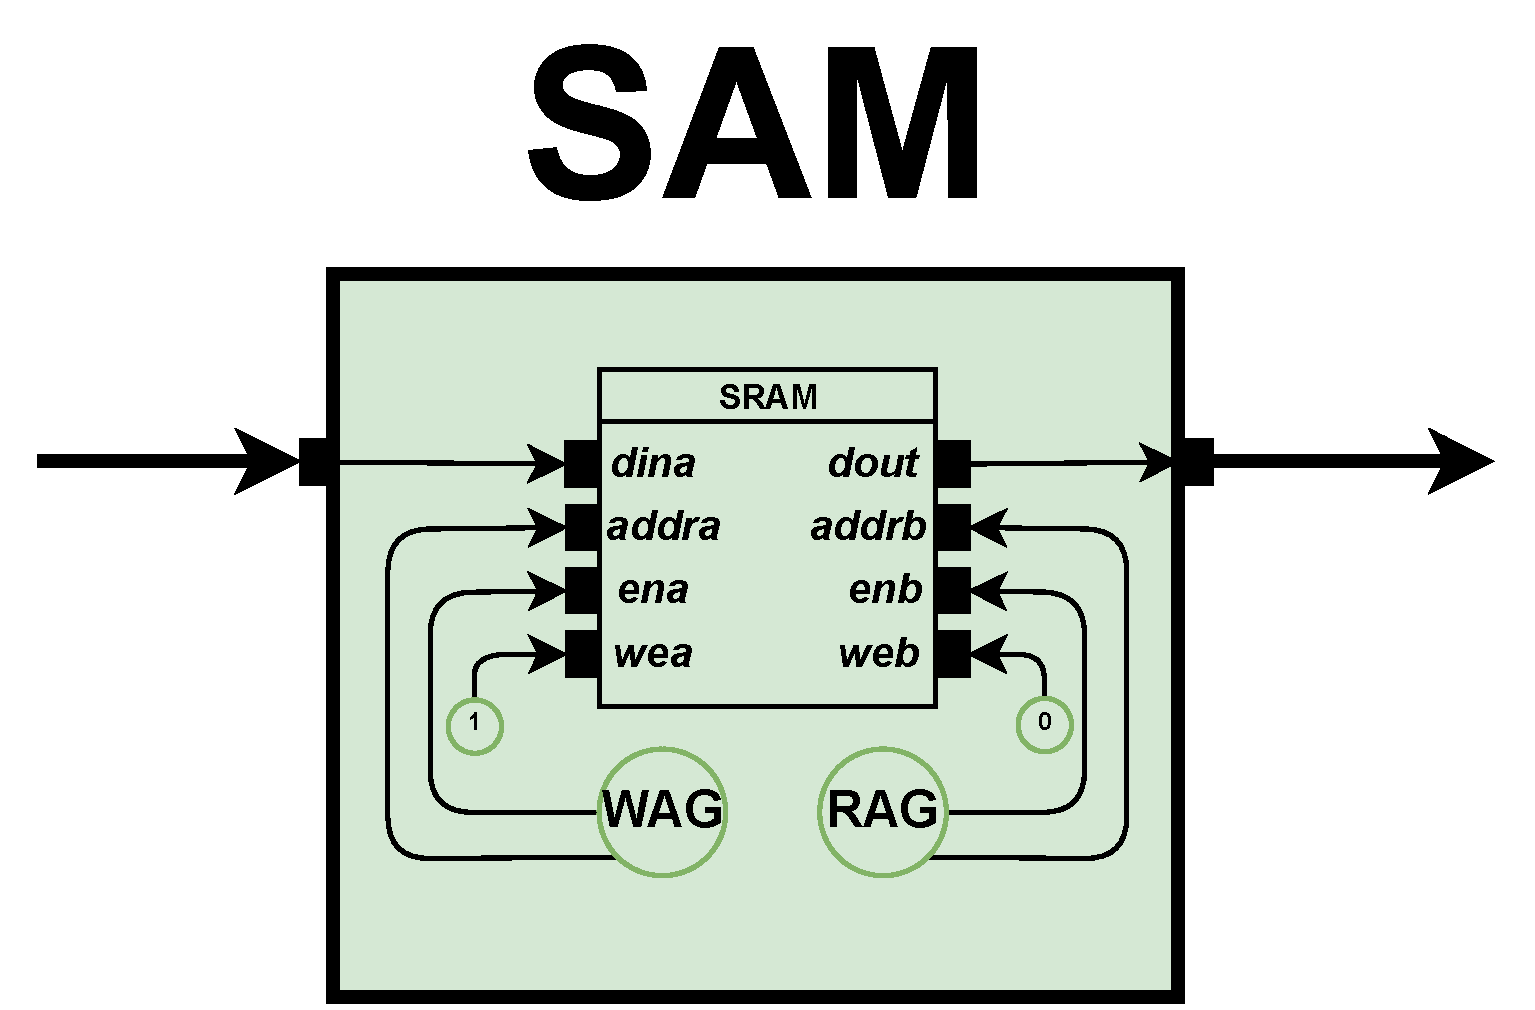
\includegraphics[width=0.495\textwidth]{fig/sam_anatomy.pdf}}
    \subfigure[]{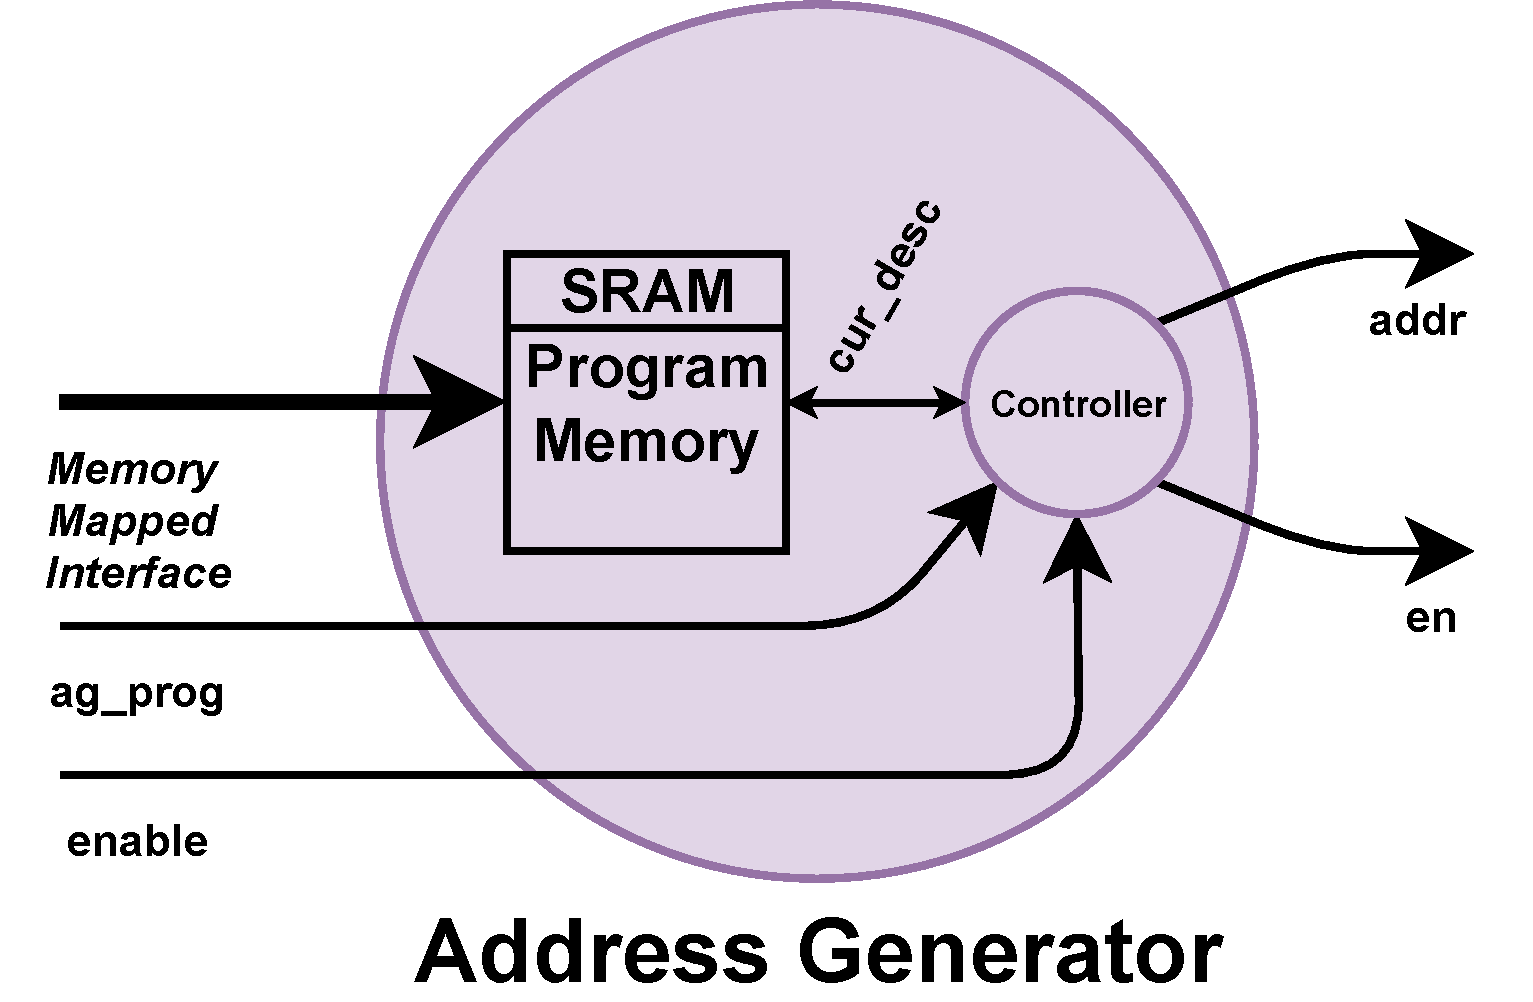
\includegraphics[width=0.495\textwidth]{fig/ag_anatomy.pdf}}
    \caption{Illustration of different dataflow implementations adapted from \cite{dnn_df_overrated} (a) blah (b) blah (c) blah (d) blah}
    \label{fig:sam_structure}
\end{figure}

In \autoref{fig:sam_structure}.a SAMS are composed of an address generator and a
data sram. Address generators are attached to ports of an SRAM. They control the
address and enable ports for each SRAM port. The port behavior (read or write)
is set by a memory mapped register attached to the write enable pins of each
port. Address generators are programmable modules within SAMs that generate address
streams based on descriptor programs. These address streams are then fed to the
SAMs data SRAM. In \autoref{fig:sam_structure}.b, address generators are
composed of a controller attached to a program memory SRAM. Depending on the
sizing requirements of the descriptor programs, program memory SRAMs can be
replaced with register files containing all relevant descriptors. SAM address
generators are equipped with an external memory mapped interface to allow
transfer of descriptor programs from an a software based co-processor.

\section{Address generator controller}
\label{chap:sams:controller}

The finite state machine of address generator controllers is presented in
\autoref{fig:ag_fsm}. After an initial reset, the controller waits until the
ag\_prog signal is asserted thus indicating that the generator is in the program
state and is awaiting to receive a descriptor based program from the external
memory mapped interface. Once the program is confirmed to be have been written
by the external interface the ag\_prog signal can be de-asserted followed by the
assertion of the enable signal. When that occurs the controller transitions into
the execute state in which it loads the first descriptor and executes it. If the
enable signal is de-asserted for any reason the controller enters a pause state.
When the enable signal is re-asserted the controller goes back to the execute
state. Once a descriptor is retired, the controller reads the next descriptor
from the program memory and begins executing it without leaving the execute
state. If the controller's cur\_desc pointer points to a suspend descriptor
execution terminates the controller enters a suspend state.

\begin{figure}
    \centering
    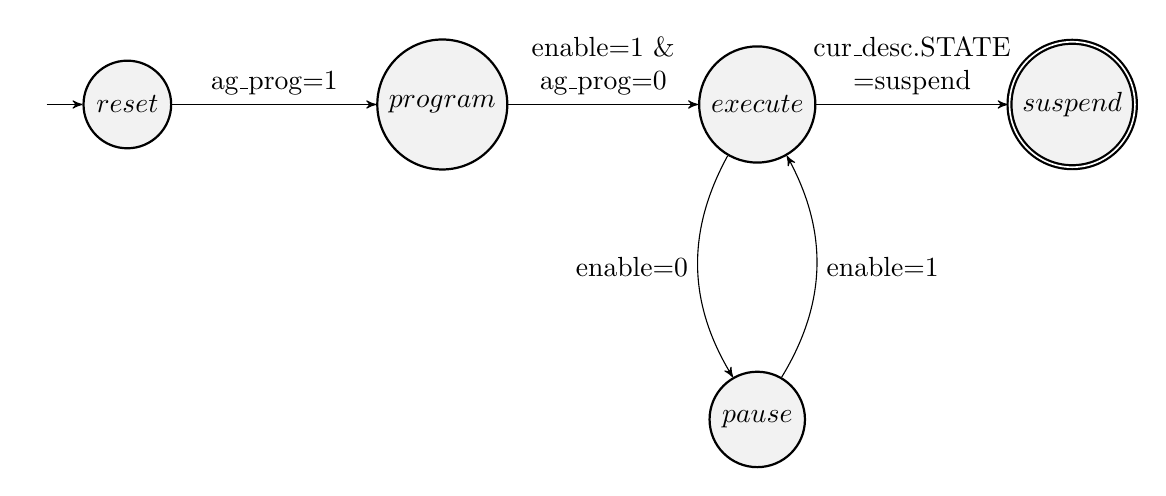
\begin{tikzpicture}
        \node[state, initial] (reset) {$reset$};
        \node[state, right of=reset] (program) {$program$};
        \node[state, right of=program] (execute) {$execute$};
        \node[state, below of=execute] (pause) {$pause$};
        \node[state, accepting, right of=execute] (suspend) {$suspend$};

        \draw   (reset) edge[above] node{ag\_prog=1} (program);
        \path[->] (program) edge[above] node[align=center] {enable=1 \&\\ag\_prog=0} (execute);
        \draw   (execute) edge[bend right, left] node{enable=0} (pause)
        (pause) edge[bend right, right] node{enable=1} (execute);
        \path[->] (execute) edge[above] node[align=center] {cur\_desc.STATE\\=suspend} (suspend);
    \end{tikzpicture}
    \caption{Address generator Finite State Machine}
    \label{fig:ag_fsm}
\end{figure}

\section{Descriptor based programs}
\label{chap:sams:programs}

Descriptor based programs are inspired by \cite{2d_dma_book} where the authors
illustrates different ways to program a model Blackfin processor's DMA using
various descriptor configurations. The main difference between this work's
approach to descriptors and \cite{2d_dma_book} is the inclusion of timing and
hybrid access/timing descriptors that allow more complicated memory transactions
to occur between SAMs.

\subsection{Descriptor Types}
\label{chap:sams:descriptor_types}

% TODO: Need to discuss nuances of descriptors being retired and how long it
% takes to switch to a new descriptor (edge cases of first descriptor vs middle
% descriptor. I remember that the first descriptor allows a dead cycle sort of
% and all descriptor retirements after that need sort of allow eager execution.
% e.g generate to generate keeps en=1 and addr jumps to start of next
% descriptor. I've completely forgotten how the SystemC model does it and there
% are definite descripencies between that and the Verilog implementation. 

Before discussing descriptor based programs we must first discuss the properties
of individual descriptors. Each descriptor can be represented as a struct as
depicted in \autoref{lst:descriptor}. In a single descriptor, the state field
describes the type of the descriptor. There are four different types of
descriptors. Generate descriptors used for generating address streams.
Stuttering descriptors used for generating stuttered address streams where the
address streams are interrupted at predefined intervals. Wait descriptors that
pause execution of descriptor based programs for a set number of cycles. Lastly,
suspend descriptors used to mark the termination of a descriptor based program.

\begin{lstlisting}[language=C, caption=Descriptor Struct, label={lst:descriptor}]
struct Descriptor
{
    DescriptorState state; 
    unsigned int start;
    unsigned int x_count;
    int x_modify;
    unsigned int y_count;
    int y_modify;
};
\end{lstlisting}

Each descriptor can be thought of as a self contained program. For generate
descriptors a C code representation for their execution behavior when they are executed
by an address generator is given in \autoref{lst:descriptor:generator}. The
output signals from the address generator "en" and "addr" are referred to as
global variables in \autoref{lst:descriptor:generator}. Suspend descriptors are
the simplest of the different descriptor types. All fields except the state
field are set to 0 in the descriptor struct. The state field is set to some
predetermined value that represents the SUSPEND state. The next simplest
descriptor is the wait descriptor which can be represented using the for loop
representation in \autoref{lst:descriptor:wait} where the SRAM port enable pin is
de-asserted and a busy loop runs for x\_count cycles. The wait descriptor is used
to synchronize different descriptor programs across SAMs as well as create timed
writes and reads to and from SAMs.

\begin{lstlisting}[language=C, caption=Descriptor as a set of loops, label={lst:descriptor:wait}]
    en = 0;
    for(int x = 0; x < x_count; x++);
\end{lstlisting}

Generate descriptors use the y\_count, and x\_count fields in the descriptor struct
to define the upper bounds for two nested loops within which an addr
variable is incremented by x\_modify in the inner loop and y\_modify in the
outer loop. The "addr" output signal is initialized with the contents of the
start field and the "en" signal is asserted for the duration of the descriptors
execution.

\begin{lstlisting}[language=C, caption=Descriptor as a set of loops, label={lst:descriptor:generator}]
en = 1;
addr = start;
for(int y = 0; y < y_count; y++)
    for(int x = 0; x < x_count; x++)
        addr += x_modify;
    addr += y_modify;
\end{lstlisting}

For stuttering descriptors, again a C code representation is given in
\autoref{lst:descriptor:stut}. As in the previous listing "addr" is initialized
with the value in the start field. However, unlike the previous listing the loop
structure of the descriptor is different. In \autoref{lst:descriptor:stut} the
outermost loop represents is bounded by the y\_count field in the descriptor
strut. Within the outer loop two loops exist, one loop dedicated to generating
the address stream based on the fields x\_count and x\_modify while the other is
dedicated to pausing for a predetermined number of cycles based on the contents
of y\_modify field. In between the nested loops the "en" is de-asserted to
disable reads/writes to the data SRAM connected to the address generator
controller.

\begin{lstlisting}[language=C, caption=Descriptor as a set of loops, label={lst:descriptor:stut}]
addr = start;
for(int y = 0; y < y\_count; y++)
    en = 1;
    for(int x = 0; x < x_count; x++)
        addr += x_modify;
    en = 0;
    for(int w = 0; w < y_modify; w++);
\end{lstlisting}

\subsection{Creating timed memory operations with descriptor programs}
\label{chap:sams:memory_transactions}

Depending on the composition of different descriptor programs one can create
timed memory operations with SAMs. An illustration of some of the possible timed
operations involving single address generators is given in
\autoref{fig:single_ag_ops}. In \autoref{fig:single_ag_ops}.a the contents of C0
are read in a loop. This is achieved by setting the y\_modify variable to -X to
reset "addr" to the start idx 0. In \autoref{fig:single_ag_ops}.b a wait
descriptor is inserted prior to the loop descriptor to introduce a delay in the
start time of the loop descriptor.

\begin{figure}
    \centering
    \subfigure[]{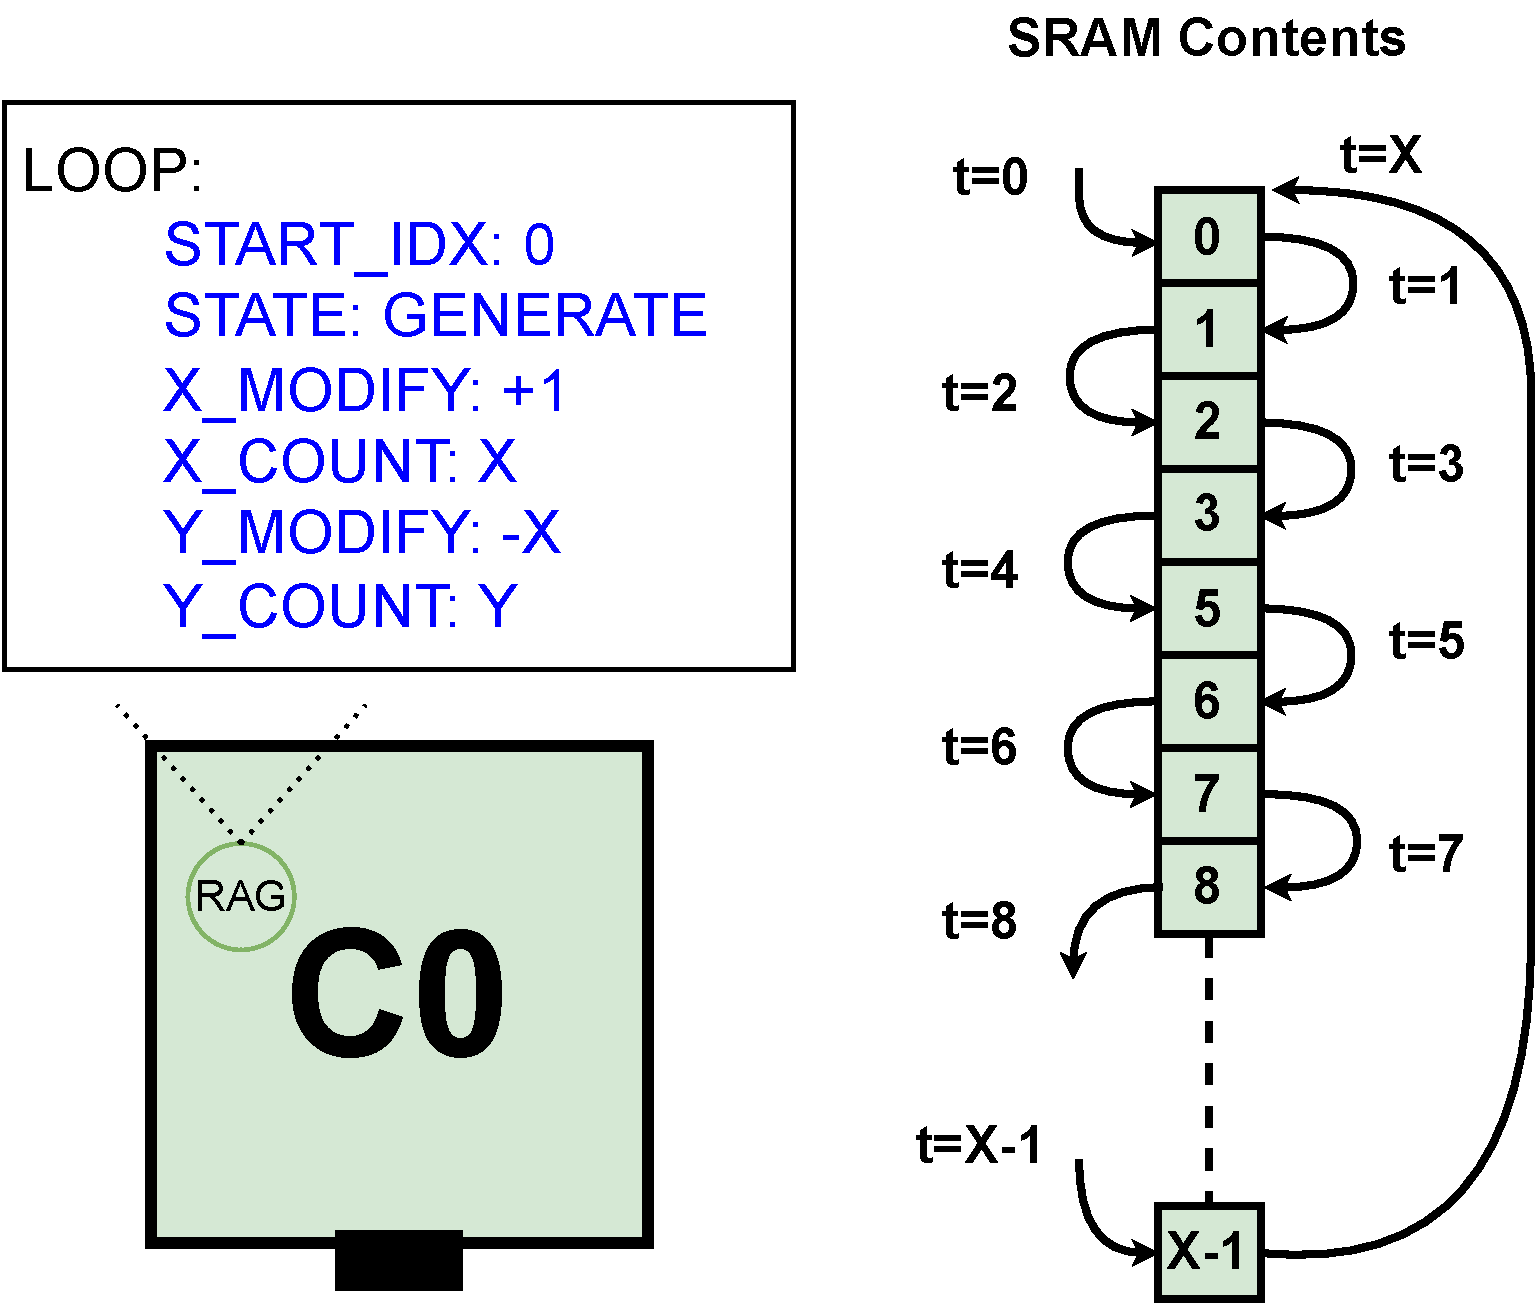
\includegraphics[width=0.4\textwidth]{fig/1D_loop_desc.pdf}}
    \hspace{0.2cm}
    \subfigure[]{\includegraphics[width=0.4\textwidth]{fig/wait_descriptor.pdf}}
    % \hspace{0.2cm} 
    % \subfigure[]{\includegraphics[width=0.25\textwidth]{fig/stutter_descriptor.pdf}}
    \caption{Illustration of different dataflow implementations adapted from \cite{dnn_df_overrated} (a) blah (b) blah (c) blah (d) blah}
    \label{fig:single_ag_ops}
\end{figure}

More complicated memory operations can be performed via the implicit
coordination of multiple address generators across SAMs or within the same SAM.
An illustration of that coordination is presented in \autoref{fig:mlti_ag_ops}.
In \autoref{fig:mlti_ag_ops}.a a data transfer between two SAMs is achieved
using one read address generator in C0 and one write address generator in C1 as
well a connection between the dout pins of C0 and dout pins of C1.
The read address generator executes a generate descriptor that reads out the
contents of the SAM. The write address generator waits for 1 cycle then executes
a write operation to store the contents of the C0 in C1. These two descriptor
programs across two SAMs implicitly coordinate with the inclusion of that wait
descriptor. They are each unaware of the program executed by the other.
Similarly this implicit coordination can occur between address generators in the
same SAM. In \autoref{fig:mlti_ag_ops}.b a read and a write address generator
coordinate to creates a shift register that reads out data received by the SAM
after a delay $\Delta_i$. This delay is introduced using similar descriptor
programs as in \autoref{fig:mlti_ag_ops}.a. In \autoref{fig:mlti_ag_ops}.b the
read address generator waits for $\Delta_i$ cycles before starting to read the
contents written by the write address generator.

\begin{figure}
    \centering
    \subfigure[]{\includegraphics[width=0.4\textwidth]{fig/sam_mem_to_mem.pdf}}
    \subfigure[]{\includegraphics[width=0.4\textwidth]{fig/sam_reuse_chain.pdf}}
    \caption{Illustration of different dataflow implementations adapted from \cite{dnn_df_overrated} (a) blah (b) blah (c) blah (d) blah}
    \label{fig:mlti_ag_ops}
\end{figure}



% \section{SAM verilog Implementation}
% \label{chap:sams:verilog_implementation}

% AXI Light was used to write descriptor programs

% Testbenches performed

% \begin{figure}
%     \centering
%     \subfigure[]{\includegraphics[width=1.1\textwidth]{fig/ag_verilog.png}} 
%     \subfigure[]{\includegraphics[width=1.1\textwidth]{fig/sam_verilog.png}}
%     \caption{Illustration of different dataflow implementations adapted from \cite{dnn_df_overrated} (a) blah (b) blah (c) blah (d) blah}
%     \label{fig:unroll_illustration}
% \end{figure}


\chapter{Network Compilation}
\label{chap:net_compile}

\section{Layer Decomposition}
\label{chap:net_compile:layer_decomposition}

Given that chip area may be restricted, a hero instance may have
insufficient on-chip storage available to hold ifmap and ofmap memory on chip
during layer processing. To minimize excessive reloads from DRAM we need a way to decompose a
larger layer into sublayers that can fit in the accelerator's on-chip memory.
Decomposition can occur due to either large ifmap or large ofmaps or in some cases
both. In this work it's assumed that decomposition occurs accross channel and
filter axis for input and output feature maps. Decomposition can occur by
decomposing large fmaps along the width and height dimentions however that
complicates the process of aggregating sub layers. This is due to the potential overlaps
of kernel windows accross decomposition boundaries. This issue arises
specifically with (3, 3) kernels under direct mode in HERO. In layers with (1,
1) kernel sizes no overlaps accross decomposition boundaries can occur due to
the small kernel size. 

Depending on the cause of layer decomposition, the dimensionality of either the
input or output featuremaps may change. Beginning with the case of decomposition due
to large ifmap tensors, \autoref{fig:ifmap_decomposition} shows how an ifmap
of size (4, 4) with 4 channels is decomposed into two separate ifmap tensors
each with 2 channels. Each sub layer consists of half the ifmap tensor. Sub
layers are processed sequentially. When
processing the second sub layer a bias is assumed to be loaded in which contains
the partial sums from the first sub layer's output. Once the second sub layer's
output is computed the final ofmap for the filter being processed becomes
available. An illustration of how ifmap decomposition affects weight tiling is
available in \autoref{fig:ifmap_decomposition:weight_tiling}. When decomposing a
large featuremap along the channel axis, the weight tensor has to also be
decomposed. Using the tiling representation of weight tensors, ifmap based
decomposition halves the size of tiles being processed by the architecture. 


\begin{figure}[ht]
    \centering
    \includegraphics[scale=0.25]{fig/ifmap_decomposition.pdf}
    \caption{Illustration of layer decomposition's effect on Ifmap tensors}
    \label{fig:ifmap_decomposition}
\end{figure}


\begin{figure}[ht]
    \centering
    \includegraphics[scale=0.4]{fig/ifmap_decomposition_tiling_repr.pdf}
    \caption{Illustration of layer decomposition's effect on weight tiling}
    \label{fig:ifmap_decomposition:weight_tiling}
\end{figure}

Decomposition due to large ofmaps follows the same logic as in the ifmap case.
An illustration of ofmap based decompsotion is available in
\autoref{fig:ofmap_decomposition:weight_tiling}. If on-chip memory is
insufficient for storing partial sums of large ofmaps from different the layer will be
decomposed into sub layers that will process only a portion of the available
filters in the layers. Ofmap based layer decomposition is also used when
processing depthwise convolution layers given that they are not supported
directly by HERO.  

\begin{figure}[ht]
    \centering
    \includegraphics[scale=0.4]{fig/ofmap_decomposition_tiling_repr.pdf}
    \caption{Illustration of layer decomposition's effect on weight tiling}
    \label{fig:ofmap_decomposition:weight_tiling}
\end{figure}

Decomposition primarily affects PE utilization since it may limit available
concurrency when processing channels and filters. In some cases it may cause a
significant reduction of PE utilization. In cases of low utilization due to
layer decomposition other forms of concurrency may need to be supported beyond
the filter/ channel/ kernel concurrency chosen by HERO. An exploration of other
forms of concurrency is left as part of future work. 

\section{Layer Scheduling}
\label{chap:net_compile:layer_scheduling}

On-chip storage requriements for ifmaps and ofmaps are influenced by the
ordering of tiles in the tiling representation of weights discussed in
\autoref{chap:dda}. The order of processing weight tiles is equivelent to the
ordering of the F, and C loops in the loop based representation of the
convolution operation discussed in \autoref{chap:dda}. Processing tiles in F, C
order (ASAP) results in retiring output featuremaps as soon as possible while retaining
input featuremaps for as long as possible. Conversly, processing tiles in C, F
order (ALAP) retains output featuremaps for as long as possible while retiring ifmaps
as soon as possible. An illustration of ASAP and ALAP tile schedules in
available in \autoref{fig:tile_scheduling}. 
% In the final template there are 4 template parameters that are customizable
% depending on the target performance/area/energy efficiency requirements of the
% acclerator. The first and the second are the unroll factors for filters
% ($F_{unroll}$) and channels ($C_{unroll}$). The third is the set of directly
% supported kernels. Finally the fourth is the spatial axis mapping of the kernel
% loops ($K_{axis}$). Each of these parameters has an effect on on-chip storage
% required for the different memories accessed.

\begin{figure}
    \centering
    \subfigure[]{\includegraphics[width=1\textwidth]{fig/asap_tiling.pdf}}
    \hspace{0.1cm} 
    \subfigure[]{\includegraphics[width=1\textwidth]{fig/alap_tiling.pdf}}
    \caption{Illustration of different tiling schedules (a) ASAP scheduling (F, C)  (b) ALAP scheduling (C, F)}
    \label{fig:tile_scheduling}
\end{figure}

An illustration of this architectural tradeoff is present
in \autoref{fig:Fmap_scaling}.c. Note that depending on the tile scheduling
chosen, different HERO template parameters affect the scaling of different
on-chip memories. For example, under ASAP, input featuremap memory requriements
remain unchanged with any template parameters, however, ofmap memory scales
with the architecture's filter unroll factor. Under ALAP ofmap memory remains
unaffected by any of HERO's template paramaters, however, ifmap memory scales
with the architecture's channel unroll factor. An illustration of how both
memories scale with tempalate paramaters is given in
\autoref{fig:Fmap_scaling}.a \& \autoref{fig:Fmap_scaling}.b. 

\begin{figure}
    \centering
    \subfigure[]{\includegraphics[width=0.45\textwidth]{Plots/ifmap_Storage.pdf}}
    \hspace{0.1cm} 
    \subfigure[]{\includegraphics[width=0.45\textwidth]{Plots/PSUM_Storage.pdf}}
    \subfigure[]{\includegraphics[width=1\textwidth]{fig/psum_ifmap_mem_scaling.pdf}}
    \caption{Illustration of storage tradeoff between OFmaps and IFmaps depending on tile scheduling (loop ordering) and accelerator template parameters (loop unroll factors) (a) IFmap storage (b) OFmap storage (c) archictural illustration}
    \label{fig:Fmap_scaling}
\end{figure}

In this work ASAP scheduling is always assumed given the relatively poor scaling
of ofmap memory with architecture template paramaters. This poor scaling is due
to the necessity of storing ofmap elements using higher precision values to
prevent numeric overflow. Note that in allowing different tile schedules may
sometimes negate the need for layer decomposition. The interaction between layer
decomposition and layer scheduling is left as part of future work.  

% While a weight stationary offers limited flexibility with regards to loop
% reoredering it does offer some degree of flexibiltiy with regards to ordering
% filter loops and channel loops. F, C loop ordering affects required on-chip
% storage for IFmaps and OFmaps.
% Under Direct mode and Gemm mode with balanced lowering, IFmap sizes
% do not exceed $2^{19.25}$ bytes (assuming 8 bit precision) for 95\% of all
% convolution layers in CIGAR's library. An estimation of the
% on-chip area required to store IFmaps using the model presented in
% \cite{area_model} yields a total on-chip area per sram bit stored equal to 0.013
% $um^2$ which translates to $0.064 mm^2$ on-chip area dedicated to sram buffers
% for storing entire input feature maps for a layer at 14nm technology.
% This area/storage does not scale with increased/decreased filter unroll factor,
% channel unroll factor or max directly supported kernel size. On-Chip area
% dedicated to storing Weights scales with the afformentioned parameters.
% Storage with regards to OFmaps depends on the loop ordering in the chosen
% dataflow. Specifically on-chip OFmap storage depends on whether filter loops and
% channel loops are reordered such that OFmaps are retired as fast as possible
% (ASAP tile scheduling) by iterating through IFmap channels first while
% processing a groups of filter, or as late as possible (ALAP tile scheduling) by
% iterating through filters first while processing a group channels. These two
% orderings for filter loops and channel loops represent different tile schedules
% for processing convolution layers. An illustration of both tile scheduling
% approaches is illustrated in \autoref{fig:tile_scheduling}. In
% \autoref{fig:tile_scheduling} a (1, 1) convolution layer's weights are shown with
% the architecture's unroll factors overlayed on top. The overlay of the
% architecture's unroll factor creates distinct weight tiles where componenets of
% the OFmap are computed. The order of executing these weight tiles depends on the
% chosen tile schedule. ASAP which represents F, C loop ordering and ALAP which
% represents C, F loop ordering. 

% A tradeoff between required IFmap storage and required OFmap storage is apparent
% in \autoref{fig:fmap_size_trends}. Under ASAP scheduling, storage requirements for
% OFmaps scales with $F_{unroll}$ because $F_{unroll}$ represents the maxmimum
% number of filters in flight. Storage requirements for IFmaps is maximized under
% ASAP because all channel data would need to be held on-chip assuming no
% additional reads can be made from DRAM for IFmap channels. Under ALAP
% scheduling, storage requirements for IFmap scale with $C_unroll$ because
% $C_{unroll}$ represents the maximum number of channels in flight. Storage for
% OFmaps is maximized under ALAP. In this thesis it is assumed that chip
% area (and thus on-chip memory) is always sufficient at least one of the
% afformentioned tile schedules without requiring loop blocking and additional
% DRAM accesses for feature maps. An exploration of the effect of loop blocking
% under more restrictive area constraints is relegated to future work. 

\clearpage

\section{Descriptor Program Generation}
\label{chap:sams:acc_scheduling}

We can generate descriptor programs for the SAMs present in
in the final architecture template for HERO discussed in \autoref{chap:dda:hw_dse:final}.
These descriptor programs will be used to perform memory operations necessary
for the convolution operation to take place in the final architectural template.
It's assumed that all on-chip SRAMs present in the HERO architecture are SAMs
capable of being programmed with descriptor based programs.   
Since we have two operational modes based on the findings of
\autoref{chap:dda} (direct and Indirect mode) we will discuss the
descriptor programs required for both of these modes to take place independently of
the other. Note that indirect mode is just a data transformation operation
followed by a (1, 1) convolution operation as discuseed in
\autoref{chap:dda:dataflow_dse:indirect_mode}. Indirect mode data
transformations (lowering/ lifting) are assumed to be performed off chip. Moving
these transformations on-chip is left as part of future work. This leaves us
with effectively two operations we need to generate descriptors for, (1, 1) and (3, 3)
convolutions. For each operation, descriptor based programs need to be generated
to perform the necessary data transfer operations between on-chip memories and
PEs. It's assumed that all on-chip SRAMs in HERO are SAMs capable of being
programmed with descriptor based memories. 
For now it's assumed that there exists two flexible interconnects for routing
control signals between address generators and on-chip SRAMS. One between all
address generators and banks in Ifmap L3 and another between all address
generators and Ofmap banks. These control interconnects are different from the
data interconnects that allow routing of data from banks to arbitrary output
ports connected PEs. An illustration of this interconnect scheme is available in
\autoref{fig:interconnect}

\begin{figure}[ht]
    \centering
    \includegraphics[scale=0.3]{fig/interconnect.pdf}
    \caption{Illustration of interconnects for control and data in on-chip featuremap memories}
    \label{fig:interconnect}
\end{figure}


This flexible interconnect for routing control signals
allows address generators of SAMs to be able to send read/write requests to
different SRAMs connected to the same interconnect which enables arbitrary
access of featuremap banks. This solution is likely not scalable to larger
instances of HERO and will be superceeded by statically scheduled control
interconnects in future work. 
Additionally, all interactions between SAMs and DRAM are left as part of future
work. IFmap and OFmap data is assumed to be read from and written to DRAM before
and after the operation of the SAM programs discussed in thi section. Latencies
and energy penalties associated with DRAM will be considered in
\autoref{chap:results} but the descriptor programs discussed in this chapter are
DRAM agnostic.

\subsection{1x1 convolution programs}
\label{chap:sams:acc_scheduling:1x1}


To illustrate how SAMs can be programmed to perform a (1, 1) convolution we will
use a simplified version of HERO illustrated in \autoref{fig:1x1conv_sched_tiling} and a (1, 1) convolution
layer with 16 channels and 8 filters as a driving example. The simplified
version of HERO assumed that there are a total of 9 processing engines with all 9
mapped to the accelerator horizontal spatial axis which enables creates an
effective an unroll factor of 9 at kernel sizes (1, 1). Based on the tiling
discussion in
\autoref{chap:dda:dataflow_dse:pruning:applying_it:loop_unroll_factors}, the
architecture tiles the weight tensor into 16 tiles (padding included) as
illustrated in \autoref{fig:1x1conv_sched_tiling}.

\begin{figure}[ht]
    \centering
    \includegraphics[scale=0.6]{fig/1x1conv_sched_tiling.pdf}
    \caption{Illustration of weight tiling under (1, 1) convolution}
    \label{fig:1x1conv_sched_tiling}
\end{figure}

For each weight in the tiles of \autoref{fig:1x1conv_sched_tiling} the channel
feature map corresponding to that weight has to be streamed into the PE
processing the output of that weight. For example, tile highlighted in red needs
channels C0-C8 streamed into the PEs storing those weights for processing. After
the red tile is processed, the green tile is loaded into the PEs weight buffer
(assuming ASAP scheduling as seen in
\autoref{chap:net_compile:layer_scheduling}). Channels C9-C15 then needs to be
streamed into the PEs holding the weights corresponding to those channels. This
means that channel memories may need to hold multiple channels that are streamed
out depending on the index of the tile being processed. An illustration of how
channel feature maps are stored on the channel SAMs is present in
\autoref{fig:channel_banking}. Note that in cases where channel featuremaps
exceed the size of one bank, layer decomposition spreads the feature map accross
multiple banks. This causes a reduction in available channel concurrency which
leads to low PE utilization. PEs holding 0 valued weights due to padding have no
corresponding channel data so nothing is streamed into them as reflected in the
0 padding of the last channel SAM attached to the 9th PE in
\autoref{fig:channel_banking}. Additionally, they are assumed to just forward
any partial sums/ output feature maps recieved from their input to their output
with no modifications.

\begin{figure}[ht]
    \centering
    \includegraphics[scale=0.495]{fig/1x1conv_ifmap_banking.pdf}
    \caption{Illustration of channel banking in Ifmap L3 on-chip SRAMs}
    \label{fig:channel_banking}
\end{figure}

Since (1, 1) convolutions involve entire channel feature maps streamed into PEs
with no reuse within a feature map occuring as in the (3, 3) case, the only
memories that need to be programmed are the L3 channel memories and the OFmap
memories. An illustration of the required descriptor programs for the
afformentioned memories is given in \autoref{fig:1x1conv_sched}. In
\autoref{fig:1x1conv_sched} hirarchy layers unused by the computatation 
as well as some PEs have been ommited to for brevity.

\begin{figure}[ht]
    \centering
    \includegraphics[scale=0.495]{fig/1x1conv_sched.pdf}
    \caption{Illustration of (1, 1) convolution scheduling}
    \label{fig:1x1conv_sched}
\end{figure}

In \autoref{fig:1x1conv_sched} channel memories can be implemented with SAMs.
For each channel SAM there are two descriptors types that appear frequently in
their programs, a wait descriptor and generate descriptor. Channel SAMs need to
perform timed reads due to the systolic delays arising from the systolic
reduction of partial sums into output feature maps. Therefore, an initial wait
instruction due to the systolic delay required by each SAM is inserted at the
begining of their descriptor programs. The delay defined by the wait descriptor
for each SAM depends on the index of the PE that the SAM is connected to. So the
first PE's corresponding SAM has no read delay so the x\_count variable in the
wait descriptor is set to 0. The next PE's channel SAM has a delay of 1 so it's
initial weight descriptor's x\_count is set to 1. After the initial wait
descriptor, each channel SAM needs to stream out a feature map. Depending on the
index of the tile being processed, each SAM streams out a different IFmap. What
distinguishes each IFmap stored on a channel SAM from another is it's start
index. For example, for the first tile highlighted in red, the first PE streams
out the IFmap begining at start index 0 with a generate descriptor. The size of
that IFmap is assumed to by $XY$ where $X$ and $Y$ are the width and height of
the IFmap. The generate descriptor increments the internal address "addr" $XY$
times with "addr" starting at 0. The corresponding generate descriptor that
manipulates the "addr" like that is a generate descriptor with an x\_count of
$XY$ and a start index of 0. When the first PE begins processing the second
tile, it reads out the IFmap stored at index $XY$ or more generally
$MOD(tile_{idx},2).XY$ since each filter has 2 tiles. This generate descriptor
is repeated for each tile in the weight tensor assuming that no padding. If a PE
is storing a 0 valued weight due to padding the generate descriptor is replaced
with a wait descriptor with an x\_count of $XY$. Optimizating descriptors to
reduce code size is left as part of future work.

For the OFmap SAM two address generators are required due to the read modify
write nature of OFmaps. The read port begins reading the layer bias immediately
and streams it into the first PE as part of partial sum reduction. All later
reads from the OFmap SAM are for partial sums that have yet to be accumulated
into OFmaps. The read descriptor required for streaming in bias/ partial sums is
a generate descriptor that streams out the contents of OFmap in a loop. It
achieves this by setting x\_count to $XY$ to stream out partial sums of size
$XY$ and y\_count to 2 which the number of tiles in a filter. To reset the
"addr" index of the read descriptor the y\_modify is set to $-XY$. This generate
descriptor is repeated 8 times where 8 is the number of filters present
processed by the PEs assuming no filter padding. Assuming ASAP tile scheduling,
OFmaps are written to DRAM as soon as they are completed and are not kept on
chip.

The write port waits for $C_{UNROLL}$ number of cycles to write the first
partial sums that will eventually become OFmaps once the filter being processed
concludes. IFmaps of $XY$ size less than 9 (the number of PEs in the horizontal
axis) will cause additional delay cycles to be introduced via wait descriptors
to allow partial sums to propogate through the PEs to reach the OFmap.
 The descriptor required for
the write address generator are similair to the the read ones with the exception
of an additional wait descriptor that gives the first partial sum/ Ofmap time to
propogate through the systolic reduction. The delay required by the wait
descriptor is equal to the number of PEs present in the horizontal axis. After
the wait descriptor comes a generate descriptor that writes the partial sum
output/ OFmap output into the OFmap SAM in a loop. The write generate
descriptor is repeated 8 times as well assuming no padding similair to
the read generate descriptor.

\subsection{3x3 convolution programs}
\label{chap:sams:acc_scheduling:3x3}

Since (3, 3) convolution operations involve the ifmap L2 vertical reuse memory,
data transfer operations between L3 an L2 have to be performed by the descriptor
based programs in memories of both layers. Thankfully, the programs for L3
memories are similair to the (1, 1) convoltuion case where each memory streams a
series of ifmap channels after a systolic delay. The main difference between (3, 3)
and (1, 1) L3 programs is is the existence of an initial setup phase where the
first two lines of a featuremap are transferred into the L2 followed by a delay
that allows partial sums to propogate down to the set of PEs each L3 featuremap
bank is connected to. Once this setup phase concludes the rest of the
featuremap is streamed out in the run phase. These two phases are repeated for every
weight tile in the layer. The L2 memory acts as a series of programmable fifos
that emit featuremaps after a delay determined by the width of the featuremap.
An illustration of this behavior is given in \autoref{fig:mlti_ag_ops}.b. 


\begin{figure}[ht]
    \centering
    \includegraphics[scale=0.495]{fig/3x3conv_sched.pdf}
    \caption{Illustration of (1, 1) convolution scheduling}
    \label{fig:3x3conv_sched}
\end{figure}


\chapter{HERO Architecture Simulation}
\label{chap:hero}

so lets say we have a concrete instance of hero-t and we want to assess its
performance in a cycle accurate simulator with real layers from a network. We do
this with a platform simulator that has a front end that takes a mode library
and produces latency, utilization and access cost results.  

\section{Simulation platform}
\label{chap:hero:sim_platform}

Sim runs a CIGAR pass over the input model library if stats dict not available.
It then performs a layer equivelence pass that converts an unsupported
convolution layer to an equivelent GEMM using balanced lowering. Overhead Of
lowering and lifting is automatically added to the overall latency of the cycle
accurate simulation. Simulation only targets conv layers. 

\begin{figure}[ht]
    \centering
    \includegraphics[scale=0.58]{fig/hero-t-sim-platform.pdf}
    \caption{Hardware Implementation Taxonomy adapted from \cite{maestro}}
    \label{fig:hw_taxonomy}
\end{figure}


\section{SystemC Model}
\label{chap:hero:sim_platform:sysc_side}

SystemC models takes in arch config. Arch config usually comes out of a tempo.
Currently systemc model only considers horizontal mapping of kernel loops. All
muxing/ interconnect logic handled with how individual banks are accessed in the
architecture simulation loops. After systemc backend recieves sim config. It
instantiates an arch with the required config. It generates an equivelent layer
following dimensions of layer sent in from front end and then it generates the
descriptor program based on the method discussed in (REFERENCE SAM SUBSECTION)
Finally the backend performs a cycle accurate simulation of the instantiated
architecture. After simulation concludes, ofmap memory contents are scanned to
validate output and if output is valid, latency, access counts and utilization
statistics are returned to the platform frontend for high level analysis. Model
is simulated in isolation. DRAM access counts are estimated in the backend but
no actual simulation of DRAM occurs.

\begin{figure}[ht]
    \centering
    \includegraphics[scale=0.58]{fig/hero-t-sysc.pdf}
    \caption{Hardware Implementation Taxonomy adapted from \cite{maestro}}
    \label{fig:hw_taxonomy}
\end{figure}


\section{Experimental Results}
\label{chap:hero:sim_platform:cigar_side}

Prominent model's convolution layers were are assessed using the simulation platform  
namely resnet-50 mobilenetv3 and vgg16. Performance for each of the three conrete
architectures suggested by tempo is reported below.

\input{tex/hero-t-sim.tex}

\chapter{Related work}
\label{chap:related_work}

\section{Convolution accelerator architectures}
 
DNN accelerator generator GEMMINI doesn't optimize for direct convolutions

GEMM Based 

TPU 

Direct 

Reduction tree based 

Maeri 

Systolic array based 

Eyeriss 
 
\section{Convolution accelerator generation techniques}

ASIC Based generators 

King Kong 

Horowitz 

Reduction tree based 

Maeri 

 


% background
%\chapter{Background}
\label{chap:background:intro}

To motivate the architecture design space introduce in chapter (REFERENCE chapter)
I first need to 
3) show how to convert a convolution operation into a GEMM
4) Introduce dataflow exploration through direct representation if implementing
an accelerates that accelerates convolutions directly
5) Introduce hardware 
+ based on reuse behavior in the Dataflow
dataflow -> describes communication -> describes datareuse
6) Introduce polyhedral model to evaluate temporal reuse behavior
In this chapter I
breakdown what convolutions are mathetmatically


\figref{fig:cnn_network}

\begin{figure}[ht]
    \centering
    \includegraphics[scale=0.4]{fig/cnn.pdf}
    \caption{Example Image Classfication CNN}
    \label{fig:cnn_network}
\end{figure}

\clearpage

\section{The Math behind convolutions}
\label{chap:intro:conv_operation}

1) explain what convolutions are mathematically

\begin{figure}[ht]
    \centering
    \includegraphics[scale=0.6]{fig/ConvExplained.pdf}
    \caption{Convolution Operation Illustrated}
    \label{fig:conv_explained}
\end{figure}

\begin{align}
    \begin{split}
        IFmap \in R^{C \times n\times n} \\
        OFmap \in  R^{F \times m\times m} \\
        Weight \in R^{F \times C\times K\times K} \\
    \end{split}
    \label{math:default_tensor_def}
\end{align}

\begin{align}
    OFmap[f][y][x] = \displaystyle\sum\limits_{c=0}^{C-1}\displaystyle\sum\limits_{k_x=0}^{K-1}\displaystyle\sum\limits_{k_y=0}^{K-1}Weight[f][c][k_y][k_x]*IFmap[c][y+ky][x+kx]
    \label{math:conv_equation_1fp}
\end{align}

\section{Loop Based Representation Of Convolutions}
\label{chap:intro:conv_operation}

Direct naive implementation of \autoref{math:conv_equation} with tensors
\autoref{math:default_tensor_def} as a series of loops is given below
\autoref{lst:conv_loop}

\begin{minipage}{\linewidth}
    \begin{lstlisting}[language=C, caption=Convolution implemented as nested loops, label={lst:conv_loop}]
for(int f = 0; f < F; f++) // Filter loop
    for(int c = 0; c < C; c++) // Channel loop
        for(int y = 0; y < Y; y++) // Output feature map row
            for(int x = 0; x < X; x++)  // Output feature map col
                for(int ky = 0; ky < KY; ky++)  // Kernel row
                    for(int kx = 0; kx < KX; kx++)  // Kernel col
                        O[f][y][x] += I[c][y+ky][x+kx]*W[f][c][ky][kx];
    \end{lstlisting}
\end{minipage}

\newpage

\section{Convolution as general matrix multiplication}
\label{chap:intro:conv_operation}

\begin{figure}[ht]
    \centering
    \includegraphics[scale=0.6]{fig/Im2Col.pdf}
    \caption{Im2Col Illustrated}
    \label{fig:im2col}
\end{figure}

Convolution can be converted into a \ac{GEMM}

Popular techniques like im2col (illustrated in \autoref{fig:im2col}) can be used
to convert any convolution operation into \ac{GEMM} (listed as expensive
lowering \cite{cafe_con_troll}) but there are others techniques that don't
produce such massive input feature maps


If willing to increase complexity of lowering of ifmap and weight tensors after
GEMM we can reduce bloat in ifmap with balanced lifting/ loading in
\cite{cafe_con_troll}. Analytical expressions adapted from \cite{cafe_con_troll}
are given below with the inclusion of lowering in the presence of multiple
filters.


\clearpage

\begin{align}
    \begin{gathered}
        IFmap \in R^{C\times n\times n} \xrightarrow[]{Balanced Lowering} \hat{IFmap} \in R^{nm\times KC} \\
        \hat{IFmap}[cn+r, :] = vec(IFmap[:, r, c:c+K]) \\
        \forall r,c \in [0, n-1], [0, m-1]
    \end{gathered}
    \label{math:balanced_lowering_ifmap}
\end{align}

\begin{align}
    \begin{gathered}
        Weight \in R^{F\times C\times K \times K} \xrightarrow[]{Balanced Lowering} \hat{Weight} \in R^{KC\times FK}\\
        \hat{Weight}[f*K:f*K+K, i] = vec(Weight[f, :, i, :]) \\
        \forall f,i \in [0, F-1], [0, K-1]
    \end{gathered}
    \label{math:balanced_lowering_weight}
\end{align}
In balanced lowering, we first lower the ifmap and weights using expression 
\eqref{math:balanced_lowering_ifmap} and \eqref{math:balanced_lowering_weight}.

\begin{align}
    \begin{gathered}
        \hat{OFmap} = \hat{IFmap}.\hat{Weight}
    \end{gathered}
    \label{math:balanced_lowering_gemm}
\end{align}
Then a \ac{GEMM} is performed \eqref{math:balanced_lowering_gemm}


\begin{align}
    \begin{gathered}
        \hat{OFmap} \in R^{nm\times FK} \xrightarrow[]{Balanced Lifting} OFmap \in  R^{m\times m\times F}\\
        OFmap[f, r, c] = (\displaystyle\sum\limits_{j=0}^{K-1} \hat{OFmap}[cn+r+j, j+fK]) \\
        \forall f,r,c \in [0, F-1], [0, m-1], [0, m-1]
    \end{gathered}
    \label{math:balanced_lifting_ofmap}
\end{align}

Followed by a lift operation on the output $\hat{OFmap}$ matrix using \eqref{math:balanced_lifting_ofmap}

Illustration of this data transformation is presented in \autoref{fig:balanced_lowering_lifting}

Pros of lowering/ lifting

Conv as GEMM Offers the most flexibility because it’s insensitive to changes in
convolution parameters

It also allows leaves us with a GEMM accelerator which is useful for many other
NN layers e.g Linear/ Self attention/ LSTM

Con is that it still causes bloat in ifmap and additionaly complexity/ latency of 
lifting/ lowering. Which in the balanced case is $m^{2}K$ \cite{cafe_con_troll}

\begin{figure}[!ht]
    \centering
    \includegraphics[scale=0.6]{fig/BalancedLoweringLifting.pdf}
    \caption{Balanced Lowering/Lifting Illustrated}
    \label{fig:balanced_lowering_lifting}
\end{figure}


\section{Implementing convolutions in hardware}
\subsection{The dataflow taxonomy}

In the dataflow design space, from \cite{dnn_df_overrated} 
dataflows can be represented using the direct convolution
nested loop structure combined with unroll pragmas. Listing \ref{lst:W_S_Generic_Loop} shows a generic
implementation of a single convolution layer as a loop structure under a weight
stationary dataflow configuration. What defines that dataflow is 1) loop unroll
targets 2) loop order 3) the unroll factors of the unrolled loops. Weight elements within a
kernel remain stationary throughout the computation of an output feature map
until a new tile of channels C\_T is loaded into the accelerator. Once the
weights within a particular channel and filter group are used to produce an
output feature map they are discarded and are only loaded again when computing
the same layer for a new input image. From listing \ref{lst:W_S_Generic_Loop} we
can see that from the loop unroll targets and loop unroll factors there are many
other possible dataflow configurations available to us outside of weight
stationary. Additionally, since accelerators are generally limited to two
spatial axis the loops of the convolution operation can be mapped to two spatial
axis. If we allow multiple convolution loops under some kernel unroll factor
KY\_T/KX\_T  to be unrolled and mapped to the same accelerator spatial axis we
can influence the effective unroll factors when performing different
convolutions of different kernel sizes other than KY\_T/KX\_T. The choice of
which loops are mapped to which spatial axis is an additional design dimension
alongside loop unrolling. To summarize, from the loop representation of
convolution accelerator dataflows we have three design space dimensions, 1) Loop
unroll targets 2) Loop unroll factors 3) Loop spatial mapping. Given the size of
this dataflow design space we will use CIGAR and Tempo to derive the common
case for convolution layers and limit the scope of the dataflow design space.

CNN layer loops + loop ordering + Loop tilings can express different
accelerators dataflows like row stationary, weight stationary, etc



\begin{minipage}{\linewidth}
    \begin{lstlisting}[language=C, caption=Convolution implemented as nested loops, label={lst:conv_loop}]
#pragma UNROLL F_T
for(int f = 0; f < F; f+=F_T) // Filter loop
#pragma UNROLL C_T
    for(int c = 0; c < C; c+=C_T) // Channel loop
#pragma UNROLL Y_T
        for(int y = 0; y < Y; y+=Y_T) // Output feature map row
#pragma UNROLL X_T
            for(int x = 0; x < X; x+=X_T)  // Output feature map col
#pragma UNROLL KY_T
                for(int ky = 0; ky < KY; ky+=KY_T)  // Kernel row
#pragma UNROLL KX_T
                    for(int kx = 0; kx < KX; kx+=KX_T)  // Kernel col
                        O[f][y][x] += I[c][y+ky][x+kx]*W[f][c][ky][kx];
    \end{lstlisting}
\end{minipage}


\begin{figure}
    \centering
    \subfigure[]{\includegraphics[width=0.32\textwidth]{fig/unroll_c_f.pdf}}
    \hspace{0.1cm} 
    \subfigure[]{\includegraphics[width=0.32\textwidth]{fig/unroll_fy_y.pdf}}
    \hspace{0.1cm} 
    \subfigure[]{\includegraphics[width=0.32\textwidth]{fig/unroll_c.pdf}} 
    \hspace{0.1cm} 
    \subfigure[]{\includegraphics[width=0.3\textwidth]{fig/buffer_description.pdf}}
    \caption{Illustration of different dataflow implementations adapted from \cite{dnn_df_overrated} (a) blah (b) blah (c) blah (d) blah}
    \label{fig:unroll_illustration}
\end{figure}


From dataflow we can derive hw implementation based on communication pattern and
reuse behavior of the individual data elements accessed in the convolution
layer.

\subsection{The Hardware Implementation taxonomy}

Figures in \autoref{fig:unroll_illustration} show different reduction/ multicast
schemes based on reuse behavior of data elements (IFmap, OFmap, Weights)
apparent in the dataflow. The space of available schemes is not limited to those
presented in \autoref{fig:unroll_illustration} though. In \cite{maestro} a
hardware taxonomy illustrated in figure \autoref{fig:hw_taxonpmy}.

\begin{figure}[ht]
    \centering
    \includegraphics[scale=0.58]{fig/hw_taxonomy.pdf}
    \caption{Hardware Implementation Taxonomy adapted from \cite{maestro}}
    \label{fig:hw_taxonomy}
\end{figure}


Depending on the dataflow described using the dataflow taxonomy (1) loop
ordering (2) unroll targets (2) loop unroll factors. The implementation options
are derived based on the type of reuse present in the dataflow. Following the
hardware implementation taxonomy presented in in \cite{maestro}, we can classify
the available hardware implementation options based on the the type of reuse is
spatial (reuse distance = 0) or temporal (reuse distance > 0) that exists for a
given data element accessed in the dataflow. Within a reuse type, depending on
the nature of the reuse, if it is read or read modify write, there are several
options for supporting the communication inferred from the reuse. To deduce the
type of reuse and overall communicaiton behavior for each data element in any
dataflow we can use the polyhedral model to detect temporal reuse. Spatial reuse
detection can be inferred directly from the loops.


\section{Analysis of data reuse with the polyhedral model}

\cite{meeus} used polyehdral model to analyse reuse within stencil based applications described
as nested loops. One important element in their approach is their program written in iscc that
can determine temporal reuse of data elements

There's the polyhedral extraction tool out there but unfortunately there's no
way to encode parallelism or loop unrolling in it without relying on compiler
pragmas. 

below is an example of this reuse applied to the gemm loops





% conclusion
\chapter{Conclusion}
\label{chap:conclude}

In this thesis a Hybrid GEMM and Direct Convolution Accelerator (HERO) was
introduced. HERO is a neural network accelerator that maintains computation
generality by supporting matrix multiplication while retaining computational
efficicency when running the common case configurations of the convolution
operation. The design of HERO was derived from data aware design process. To
direct that process a (ConvolutIon statIstics GAtherer) \ac{CIGAR} tool was used
to find the common case of the convolution operation that needed to be support
by HERO directly. To find optimal configurations of HERO, a HERO accelerator
TEMPlate Optimizer (TEMPO) was introduced. TEMPO was driven by an analytical
model used to maximize on-chip PE utilization. Additionally, a novel descriptor
driven on-chip memory primitive capable of orchestrating energy efficient on
chip data movements within \ac{HERO} was presented. To compile arbitrary pytorch
models down to SAM descriptors a HERO layer compiler was discussed. To estimate
the performance and energy efficiency of arbitrary HERO configurations a cycle
accurate simulation platform driven by a SystemC simulation backend and a python
evaluation frontend was developed. Finally, an analysis of an optimal HERO
configuration when running 695 networks in the TIMM library was discussed.

HERO was found to perform well on a wide variety of network configurations. It
achieved a median FPS of ~91 FPS with a median speedup of 4.87X over CPU
baseline. The estimated bandwidth required for the configuration of HERO studied
was 19.65GiB which is within the PC4-21300 DDR4 specification. With that
configuration of DRAM the median inferences/J is 57. The total on-chip area is
estimated at 0.34 $mm^2$. 

In terms of utilization, the optimal configuration found by TEMPO enables some
networks to benefit substantiatlly from HERO while others less so. Instances of
poor layer mapping to HERO include depthwise and group convolution layers that
were not considered when developing HERO as well as lowered layers that required more
compute resources than what was available in the configuration studied. 

To further the development of HERO explicit support of depthwise and grouped
convolution layers is necessary along with an exploration of alternative forms
of concurrency within HERO. Additionally, more convolution layer configurations
need to be supported directly in HERO, specifically convolution layers with a
stride size greater than 1. Along with increasing convolution support, support
for other layer types like Batch normalization layers and activation layers
needs to be included in HERO to minimize data movement between the CPU and HERO.
Similarly, lowering and lifting transformation required to extend support to
arbitrary convolution layers needs to be incorporated into HERO to minimize
off-chip datamovement. Finally a larger scale exploration of different HERO
architectures using the developed simulation platform is required to validate
and refine TEMPO's analytical model.


% --- Bibliography ----
\bibliographystyle{plain}

% include bibliography definition
\bibliography{bib/thesis}


% --- Appendix ---
\appendix
%include anything you need in the appendix
%\begin{table}[]
    \begin{tabular}{ll}
    Big Transfer ResNetV2 (BiT)                                              & \cite{srinivas_bottleneck_2021}          \\
    Bottleneck Transformers                                                  & \cite{kolesnikov_big_2020}               \\
    CaiT (Class-Attention in Image Transformers)                             & \cite{DBLP:journals/corr/abs-2103-17239} \\
    CoaT (Co-Scale Conv-Attentional Image Transformers)                      & \cite{xu_co-scale_2021}                  \\
    ConViT (Soft Convolutional Inductive Biases Vision                       & \cite{dascoli_convit_2021}               \\
    CspNet (Cross-Stage Partial Networks)                                    & \cite{wang_cspnet_2019}                  \\
    DeiT (Vision Transformer)                                                & \cite{dascoli_convit_2021}               \\
    DenseNet                                                                 & \cite{DBLP:journals/corr/HuangLW16a}     \\
    DLA                                                                      & \cite{yu_deep_2019}                      \\
    DPN (Dual-Path Network)                                                  & \cite{chen_dual_2017}                    \\
    EfficientNet NoisyStudent (B0-B7, L2)                                    & \cite{xie_self-training_2020}            \\
    EfficientNet AdvProp (B0-B8)                                             & \cite{xie_adversarial_2020}              \\
    EfficientNet (B0-B7)                                                     & \cite{tan_efficientnet_2020}             \\
    EfficientNet-EdgeTPU (S, M, L)                                           & \cite{google_ai_blog_2019}               \\
    EfficientNet V2                                                          & \cite{tan_efficientnetv2_2021}           \\
    FBNet-C                                                                  & \cite{wu_fbnet_2019}                     \\
    MixNet                                                                   & \cite{tan_mixconv_2019}                  \\
    MNASNet B1, A1 (Squeeze-Excite), and Small                               & \cite{tan_mnasnet_2019}                  \\
    MobileNet-V2                                                             & \cite{sandler_mobilenetv2_2019}          \\
    Single-Path NAS                                                          & \cite{stamoulis_single-path_2019}        \\
    GhostNet                                                                 & \cite{han_ghostnet_2020}                 \\
    gMLP                                                                     & \cite{liu_pay_2021}                      \\
    GPU-Efficient Networks                                                   & \cite{lin_neural_2020}                   \\
    Halo Nets                                                                & \cite{vaswani_scaling_2021}              \\
    HardCoRe-NAS                                                             & \cite{nayman_hardcore-nas_2021}          \\
    HRNet                                                                    & \cite{wang_deep_2020}                    \\
    Inception-V3                                                             & \cite{szegedy_rethinking_2015}           \\
    Inception-ResNet-V2 and Inception-V4                                     & \cite{szegedy_inception-v4_2016}         \\
    Lambda Networks                                                          & \cite{bello_lambdanetworks_2021}         \\
    MLP-Mixer                                                                & \cite{tolstikhin_mlp-mixer_2021}         \\
    MobileNet-V3 (MBConvNet w/ Efficient Head)                               & \cite{howard_searching_2019}             \\
    NASNet-A                                                                 & \cite{zoph_learning_2018}                \\
    NFNet-F                                                                  & \cite{brock_high-performance_2021}       \\
    NF-RegNet / NF-ResNet                                                    & \cite{brock_characterizing_2021}         \\
    \end{tabular}
    \end{table}
    \begin{table}[]
    \begin{tabular}{ll}
    PNasNet                                                                  & \cite{liu_progressive_2018}              \\
    Pooling-based Vision Transformer (PiT)                                   & \cite{heo_rethinking_2021}               \\
    RegNet                                                                   & \cite{radosavovic_designing_2020}        \\
    RepVGG                                                                   & \cite{ding_repvgg_2021}                  \\
    ResMLP                                                                   & \cite{touvron_resmlp_2021}               \\
    ResNet (v1b/v1.5)                                                        & \cite{he_deep_2015}                      \\
    ResNeXt                                                                  & \cite{xie_aggregated_2017}               \\
    Bag of Tricks' / Gluon C, D, E, S variations                             & \cite{he_bag_2018}                       \\
    Weakly-supervised (WSL) Instagram pretrained / ImageNet tuned ResNeXt101 & \cite{mahajan_exploring_2018}            \\
    Semi-supervised (SSL) / Semi-weakly Supervised (SWSL) ResNet/ResNeXts    & \cite{yalniz_billion-scale_2019}         \\
    ECA-Net (ECAResNet)                                                      & \cite{DBLP:journals/corr/abs-1910-03151} \\
    Squeeze-and-Excitation Networks (SEResNet)                               & \cite{hu_squeeze-and-excitation_2019}    \\
    ResNet-RS                                                                & \cite{bello_revisiting_2021}             \\
    Res2Net                                                                  & \cite{gao_res2net_2021}                  \\
    ResNeSt                                                                  & \cite{zhang_resnest_2020}                \\
    ReXNet                                                                   & \cite{han_rethinking_2021}               \\
    SelecSLS                                                                 & \cite{mehta_xnect_2020}                  \\
    Selective Kernel Networks                                                & \cite{li_selective_2019}                 \\
    Swin Transformer                                                         & \cite{liu_swin_2021}                     \\
    Transformer-iN-Transformer (TNT)                                         & \cite{han_transformer_2021}              \\
    TResNet                                                                  & \cite{ridnik_tresnet_2020}               \\
    Twins (Spatial Attention in Vision Transformers)                         & \cite{DBLP:journals/corr/abs-2104-13840} \\
    Vision Transformer                                                       & \cite{dosovitskiy_image_2021}            \\
    VovNet V2 and V1                                                         & \cite{lee_centermask_2020}               \\
    Xception                                                                 & \cite{chollet_xception_2017}             \\
    Xception (Modified Aligned, TF)                                          & \cite{chen_encoder-decoder_2018}         \\
    SSD                                                                      & \cite{DBLP:journals/corr/LiuAESR15}      \\
    lenet                                                                    & \cite{Lecun1998}                         \\
    YoloV5                                                                   & \cite{DBLP:journals/corr/abs-2108-11539} \\
    Alexnet                                                                  & \cite{NIPS2012_c399862d}                 \\
    SqueezeNet                                                               & \cite{DBLP:journals/corr/IandolaMAHDK16} \\
    Shufflenet                                                               & \cite{DBLP:journals/corr/ZhangZLS17}    
    VGG16                                                                    & \cite{dnn_is_sota_image}    
    \end{tabular}
    \end{table}


% --- Index ----
\printindex


% --- that's it ---
\end{document}

% --- EOF --------------------------------------------------------------------

